\documentclass[11pt,a4paper]{article}
\usepackage[margin=18mm,headheight=15pt]{geometry}
\usepackage[T1]{fontenc}\usepackage{mathpazo}
\usepackage{microtype,booktabs,array,longtable,xcolor,xurl,fancyhdr,enumitem,tikz}
\definecolor{navy}{HTML}{183047}\definecolor{teal}{HTML}{206676}\definecolor{muted}{HTML}{586775}
\definecolor{frontcu}{HTML}{C84C4C}\definecolor{backcu}{HTML}{267C84}\definecolor{boardbg}{HTML}{F6F8F8}
\usepackage[colorlinks=true,linkcolor=navy,urlcolor=teal,pdftitle={FPGA 100T - 33 x 36 mm routed revision: components and complete pin ledger},pdfauthor={FPGA 4K engineering review}]{hyperref}
\newcolumntype{P}[1]{>{\raggedright\arraybackslash}p{#1}}
\urlstyle{same}\setlength{\parindent}{0pt}\setlength{\parskip}{6pt}\setlength{\emergencystretch}{2em}
\setlist{nosep,leftmargin=5mm}
\pagestyle{fancy}\fancyhf{}\fancyhead[L]{\small\textcolor{navy}{FPGA 4K / 100T}}
\fancyhead[R]{\small\textcolor{muted}{26 September 2026 / Routed revision}}
\fancyfoot[L]{\footnotesize Partial routing checkpoint -- not for manufacture}\fancyfoot[R]{\thepage}
\renewcommand{\headrulewidth}{0.3pt}\renewcommand{\footrulewidth}{0pt}
\begin{document}
{\color{teal}\large ENGINEERING REVIEW / 2026-09-26}\par
{\color{navy}\fontsize{28}{32}\selectfont Smallest FPGA board\\[3pt]Components and every pin}\par
{\large XC7A100T, CSG324 / 15 $\times$ 15 mm package}\par\vspace{3mm}
\textbf{Current result: a 33 $\times$ 36 mm board with 130 physical components, 1,139 track segments, 164 vias and four filled ground zones.} All 25 boot/clock/programming nets and three power-good nets (two sequencing nets and one unconsumed status net) are connected in the native checks. The outline remains the smallest published version.

\textbf{It is still electrically incomplete.} There are 146 remaining power/ground connections, including seven BGA ground groups and the U4 pin 11 VSEL ground strap. All 120 mezzanine signal contacts remain unassigned. Zero physical DRC violations and zero schematic-parity issues do not establish working hardware or fabrication readiness.

This report explains every retained component and lists every numbered electrical endpoint. It replaces the earlier placement-only report for current review, while preserving that dated report as historical evidence. It focuses only on the current smallest board.

\begingroup\fontsize{9}{11.5}\selectfont\setlength{\tabcolsep}{2.8pt}\renewcommand{\arraystretch}{1.06}
\begin{longtable}{@{}P{38mm}P{43mm}P{87mm}@{}}
\toprule \textbf{Current board} & \textbf{Verified result} & \textbf{Interpretation} \\ \midrule
\endfirsthead\toprule \textbf{Current board} & \textbf{Verified result} & \textbf{Interpretation} \\ \midrule
\endhead\midrule\multicolumn{3}{r}{\small Continued on next page}\endfoot\bottomrule\endlastfoot
Outline / layers & 33 $\times$ 36 mm / 6 & 39 front and 91 back components; no assembly or stackup qualification claimed. \\
Components / endpoints & 130 / 762 & Every component and distinct numbered endpoint appears in the appendices. \\
Tracks / vias / zones & 1,139 / 164 / 4 & Real copper is present. Global power/ground routing remains unfinished. \\
Physical DRC / parity & 0 / 0 & Native checks, unchanged rules, no exclusions or ignored checks. \\
Remaining connections & 146 & Seven power/ground nets; not a percentage-complete metric. \\
ASIC interfaces & 120 unassigned contacts & 117-signal allocation remains a proposal; three contacts are reserved. \\
\end{longtable}\endgroup

\textbf{Read the status column carefully.} ``C'' means the entire named net is connected in native DRC. ``P'' means the net still has at least one open connection; it does not assert that this particular pad is disconnected. ``U'' is unassigned. ``NC'' is an intentional no-connect.
\clearpage\tableofcontents\clearpage
\section{The current small board}
\begin{center}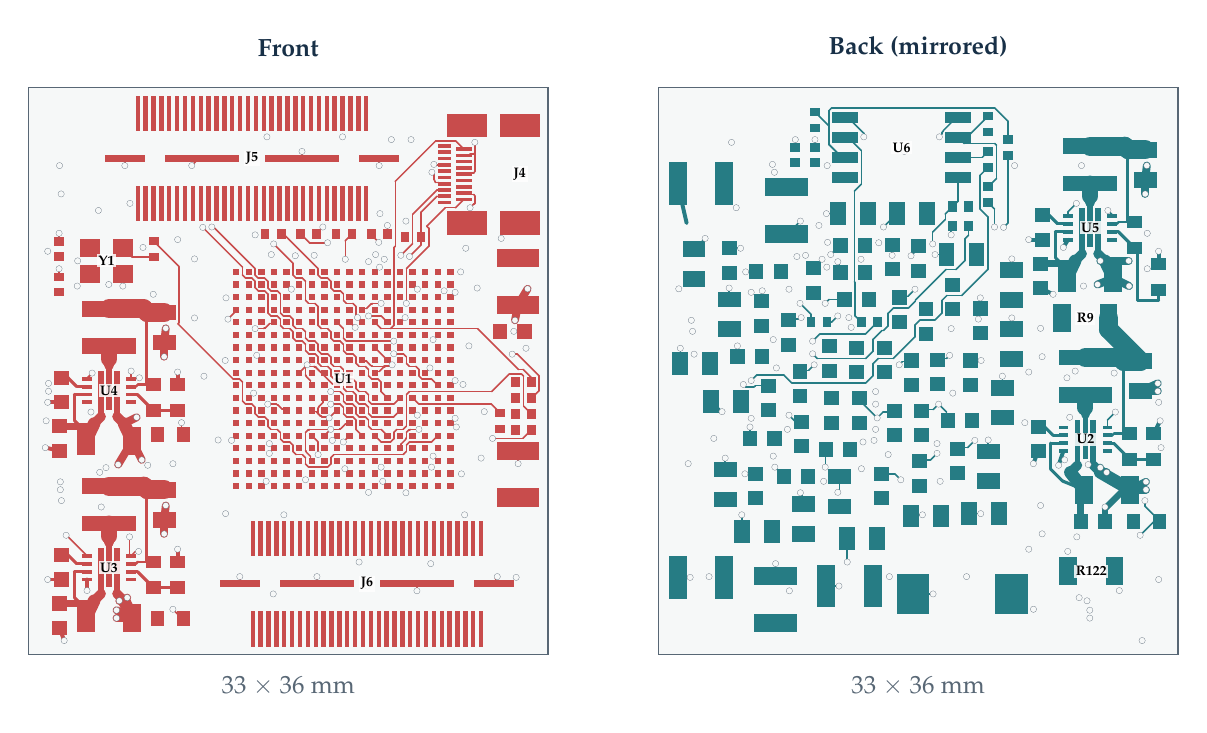
\begin{tikzpicture}[x=0.20cm,y=-0.20cm]
\begin{scope}[shift={(0,0)}]
\fill[boardbg] (0,0) rectangle (33,36);
\draw[muted,line width=.5pt] (0,0) rectangle (33,36);
\node[anchor=south,font=\small\bfseries,text=navy] at (16.5,-1.3) {Front};
\draw[frontcu,line width=0.4000mm,line cap=round] (3.075000,18.985000) -- (2.525000,18.435000);
\draw[frontcu,line width=0.4000mm,line cap=round] (2.525000,18.435000) -- (2.125000,18.435000);
\draw[frontcu,line width=0.4000mm,line cap=round] (3.725000,18.985000) -- (3.075000,18.985000);
\draw[frontcu,line width=0.2000mm,line cap=round] (14.950000,15.300000) -- (14.400000,15.300000);
\draw[frontcu,line width=0.2000mm,line cap=round] (22.075000,18.100000) -- (22.150000,18.025000);
\draw[frontcu,line width=0.2000mm,line cap=round] (17.850000,21.700000) -- (19.200000,21.700000);
\draw[frontcu,line width=0.7000mm,line cap=round] (5.625000,19.235000) -- (5.625000,20.885000);
\draw[frontcu,line width=0.2000mm,line cap=round] (21.200000,17.300000) -- (21.275000,17.300000);
\draw[frontcu,line width=0.2000mm,line cap=round] (28.050000,4.225000) -- (28.275000,4.225000);
\draw[frontcu,line width=0.2000mm,line cap=round] (6.125000,4.500000) -- (6.125000,4.950000);
\draw[frontcu,line width=0.2000mm,line cap=round] (19.775000,21.675000) -- (19.750000,21.700000);
\draw[frontcu,line width=0.2000mm,line cap=round] (18.800000,21.275000) -- (19.100000,20.975000);
\draw[frontcu,line width=0.2000mm,line cap=round] (28.050000,5.425000) -- (28.275000,5.425000);
\draw[frontcu,line width=0.2000mm,line cap=round] (18.400000,20.350000) -- (18.400000,20.700000);
\draw[frontcu,line width=0.2000mm,line cap=round] (25.875000,6.025000) -- (25.825000,5.975000);
\draw[frontcu,line width=0.2000mm,line cap=round] (18.200000,17.725000) -- (18.175000,17.725000);
\draw[frontcu,line width=0.2000mm,line cap=round] (24.000000,21.900000) -- (24.150000,21.750000);
\draw[frontcu,line width=0.2000mm,line cap=round] (17.825000,21.725000) -- (17.850000,21.700000);
\draw[frontcu,line width=0.2000mm,line cap=round] (18.075000,20.500000) -- (18.150000,20.575000);
\draw[frontcu,line width=0.2000mm,line cap=round] (19.575000,20.500000) -- (19.100000,20.975000);
\draw[frontcu,line width=0.2000mm,line cap=round] (28.275000,6.775000) -- (28.325000,6.825000);
\draw[frontcu,line width=0.2000mm,line cap=round] (23.975000,22.275000) -- (24.000000,22.250000);
\draw[frontcu,line width=0.2000mm,line cap=round] (22.800000,9.300000) -- (22.800000,8.750000);
\draw[frontcu,line width=0.2000mm,line cap=round] (18.425000,20.300000) -- (18.425000,20.325000);
\draw[frontcu,line width=0.2000mm,line cap=round] (6.135000,4.500000) -- (6.125000,4.500000);
\draw[frontcu,line width=0.2000mm,line cap=round] (24.675000,31.500000) -- (24.675000,31.950000);
\draw[frontcu,line width=0.2000mm,line cap=round] (28.375000,3.500000) -- (28.350000,3.475000);
\draw[frontcu,line width=0.2000mm,line cap=round] (18.600000,20.875000) -- (18.625000,20.875000);
\draw[frontcu,line width=0.2000mm,line cap=round] (18.200000,17.725000) -- (18.175000,17.725000);
\draw[frontcu,line width=0.2000mm,line cap=round] (18.250000,17.750000) -- (18.225000,17.750000);
\draw[frontcu,line width=0.2000mm,line cap=round] (17.600000,23.050000) -- (17.600000,21.900000);
\draw[frontcu,line width=0.2000mm,line cap=round] (18.450000,20.275000) -- (18.425000,20.300000);
\draw[frontcu,line width=0.2000mm,line cap=round] (11.025000,4.500000) -- (10.950000,4.500000);
\draw[frontcu,line width=0.2000mm,line cap=round] (28.350000,4.075000) -- (28.375000,4.050000);
\draw[frontcu,line width=0.2000mm,line cap=round] (17.625000,18.300000) -- (17.625000,18.275000);
\draw[frontcu,line width=0.2000mm,line cap=round] (17.750000,21.750000) -- (17.775000,21.750000);
\draw[frontcu,line width=0.5000mm,line cap=round] (2.125000,19.985000) -- (1.225000,19.985000);
\draw[frontcu,line width=0.2000mm,line cap=round] (19.450000,18.825000) -- (19.325000,18.825000);
\draw[frontcu,line width=1.2000mm,line cap=round] (5.625000,32.134999) -- (6.075000,32.585000);
\draw[frontcu,line width=0.2000mm,line cap=round] (27.650000,6.700000) -- (27.800000,6.700000);
\draw[frontcu,line width=0.2000mm,line cap=round] (18.625000,20.875000) -- (18.650000,20.900000);
\draw[frontcu,line width=0.2000mm,line cap=round] (22.625000,17.725000) -- (22.650000,17.700000);
\draw[frontcu,line width=0.2000mm,line cap=round] (22.810000,9.300000) -- (22.800000,9.300000);
\draw[frontcu,line width=0.2000mm,line cap=round] (18.575000,20.850000) -- (18.600000,20.875000);
\draw[frontcu,line width=0.2000mm,line cap=round] (19.025000,20.900000) -- (19.100000,20.975000);
\draw[frontcu,line width=0.2000mm,line cap=round] (28.050000,6.775000) -- (28.275000,6.775000);
\draw[frontcu,line width=0.2000mm,line cap=round] (21.850000,17.700000) -- (22.575000,17.700000);
\draw[frontcu,line width=0.2000mm,line cap=round] (29.650000,31.350000) -- (29.650000,31.175000);
\draw[frontcu,line width=0.2000mm,line cap=round] (31.100001,23.075000) -- (31.100000,23.075000);
\draw[frontcu,line width=0.2000mm,line cap=round] (25.825000,5.950000) -- (25.800000,5.925000);
\draw[frontcu,line width=0.2000mm,line cap=round] (18.725000,18.100000) -- (18.650000,18.025000);
\draw[frontcu,line width=0.2000mm,line cap=round] (28.025000,5.450000) -- (28.050000,5.425000);
\draw[frontcu,line width=1.0000mm,line cap=round] (8.625000,27.435000) -- (8.625000,28.335000);
\draw[frontcu,line width=0.2000mm,line cap=round] (19.600000,18.900000) -- (19.525000,18.900000);
\draw[frontcu,line width=0.2000mm,line cap=round] (17.800000,17.700000) -- (17.700000,17.600000);
\draw[frontcu,line width=0.2000mm,line cap=round] (24.175000,21.750000) -- (24.200000,21.725000);
\draw[frontcu,line width=1.0000mm,line cap=round] (31.100000,13.775000) -- (31.700000,12.775000);
\draw[frontcu,line width=0.2000mm,line cap=round] (21.350000,14.025000) -- (21.475000,14.025000);
\draw[frontcu,line width=0.2000mm,line cap=round] (18.450000,20.250000) -- (18.450000,20.275000);
\draw[frontcu,line width=0.2000mm,line cap=round] (23.600000,22.900000) -- (23.600000,22.825000);
\draw[frontcu,line width=0.2000mm,line cap=round] (21.850000,13.700000) -- (22.400000,13.700000);
\draw[frontcu,line width=0.2000mm,line cap=round] (28.375000,6.950000) -- (28.375000,7.325000);
\draw[frontcu,line width=0.2000mm,line cap=round] (28.325000,4.150000) -- (28.350000,4.125000);
\draw[frontcu,line width=0.2000mm,line cap=round] (18.800000,18.100000) -- (18.725000,18.100000);
\draw[frontcu,line width=0.2000mm,line cap=round] (13.425000,31.500000) -- (13.425000,31.050000);
\draw[frontcu,line width=0.2000mm,line cap=round] (19.325000,18.825000) -- (18.250000,17.750000);
\draw[frontcu,line width=0.2000mm,line cap=round] (21.475000,14.025000) -- (21.750000,13.750000);
\draw[frontcu,line width=0.2000mm,line cap=round] (22.000000,11.700000) -- (22.300000,11.400000);
\draw[frontcu,line width=0.2000mm,line cap=round] (27.850000,4.250000) -- (28.025000,4.250000);
\draw[frontcu,line width=0.2000mm,line cap=round] (31.505000,15.480000) -- (31.500000,15.475000);
\draw[frontcu,line width=0.2000mm,line cap=round] (22.575000,17.700000) -- (22.600000,17.675000);
\draw[frontcu,line width=0.2000mm,line cap=round] (18.800000,21.300000) -- (18.800000,21.275000);
\draw[frontcu,line width=0.7000mm,line cap=round] (5.625000,30.485000) -- (5.625000,32.134999);
\draw[frontcu,line width=0.2000mm,line cap=round] (18.800000,22.100000) -- (19.200000,21.700000);
\draw[frontcu,line width=0.2000mm,line cap=round] (14.800000,17.300000) -- (14.500000,17.000000);
\draw[frontcu,line width=1.0000mm,line cap=round] (6.075000,32.585000) -- (5.775000,32.585000);
\draw[frontcu,line width=0.2000mm,line cap=round] (26.800000,21.300000) -- (27.100000,21.000000);
\draw[frontcu,line width=0.2000mm,line cap=round] (28.325000,5.350000) -- (28.350000,5.325000);
\draw[frontcu,line width=0.2000mm,line cap=round] (15.825000,20.150000) -- (15.800000,20.125000);
\draw[frontcu,line width=0.2000mm,line cap=round] (18.000000,20.500000) -- (18.075000,20.500000);
\draw[frontcu,line width=0.2000mm,line cap=round] (18.310000,9.300000) -- (18.300000,9.300000);
\draw[frontcu,line width=1.0000mm,line cap=round] (6.075000,32.585000) -- (6.275000,32.384999);
\draw[frontcu,line width=0.2000mm,line cap=round] (10.875000,4.575000) -- (10.750000,4.575000);
\draw[frontcu,line width=0.2000mm,line cap=round] (20.400000,24.500000) -- (20.100000,24.200000);
\draw[frontcu,line width=0.2000mm,line cap=round] (26.000000,23.700000) -- (25.700000,23.400000);
\draw[frontcu,line width=0.2000mm,line cap=round] (24.225000,21.725000) -- (24.250000,21.700000);
\draw[frontcu,line width=0.2000mm,line cap=round] (28.350000,6.925000) -- (28.375000,6.950000);
\draw[frontcu,line width=0.2000mm,line cap=round] (25.775000,5.525000) -- (25.625000,5.375000);
\draw[frontcu,line width=1.0000mm,line cap=round] (6.600000,33.684999) -- (5.600000,33.684999);
\draw[frontcu,line width=0.2000mm,line cap=round] (17.600000,17.700000) -- (17.700000,17.600000);
\draw[frontcu,line width=0.2000mm,line cap=round] (17.775000,21.750000) -- (17.800000,21.725000);
\draw[frontcu,line width=0.2000mm,line cap=round] (23.025000,17.675000) -- (23.100000,17.600000);
\draw[frontcu,line width=0.2000mm,line cap=round] (25.800000,5.925000) -- (25.800000,5.875000);
\draw[frontcu,line width=0.2000mm,line cap=round] (17.375000,4.500000) -- (17.375000,4.050000);
\draw[frontcu,line width=0.2000mm,line cap=round] (1.960000,12.020001) -- (1.950000,12.025000);
\draw[frontcu,line width=0.2000mm,line cap=round] (19.050000,20.925000) -- (19.100000,20.975000);
\draw[frontcu,line width=0.5000mm,line cap=round] (3.725000,31.235000) -- (3.725000,31.935000);
\draw[frontcu,line width=1.0000mm,line cap=round] (6.600000,33.684999) -- (5.600000,33.184998);
\draw[frontcu,line width=0.2000mm,line cap=round] (16.125000,20.425000) -- (15.850000,20.150000);
\draw[frontcu,line width=0.2000mm,line cap=round] (27.800000,6.700000) -- (27.850000,6.750000);
\draw[frontcu,line width=0.2000mm,line cap=round] (18.150000,20.575000) -- (18.275000,20.575000);
\draw[frontcu,line width=0.2000mm,line cap=round] (23.675000,22.750000) -- (23.675000,22.625000);
\draw[frontcu,line width=0.2000mm,line cap=round] (24.400000,20.500000) -- (24.700000,20.800000);
\draw[frontcu,line width=0.2000mm,line cap=round] (26.800000,13.300000) -- (27.100000,13.000000);
\draw[frontcu,line width=0.2000mm,line cap=round] (18.000000,18.900000) -- (18.000000,18.825000);
\draw[frontcu,line width=0.2000mm,line cap=round] (17.800000,17.700000) -- (17.700000,17.600000);
\draw[frontcu,line width=0.2000mm,line cap=round] (18.575000,20.850000) -- (18.600000,20.875000);
\draw[frontcu,line width=0.2000mm,line cap=round] (22.550000,17.750000) -- (22.575000,17.750000);
\draw[frontcu,line width=0.2000mm,line cap=round] (15.025000,15.250000) -- (15.000000,15.275000);
\draw[frontcu,line width=0.2000mm,line cap=round] (28.325000,5.375000) -- (28.325000,5.350000);
\draw[frontcu,line width=0.2000mm,line cap=round] (19.800000,21.675000) -- (19.775000,21.675000);
\draw[frontcu,line width=0.2000mm,line cap=round] (28.275000,5.425000) -- (28.325000,5.375000);
\draw[frontcu,line width=0.2000mm,line cap=round] (15.050000,15.250000) -- (15.025000,15.250000);
\draw[frontcu,line width=0.2000mm,line cap=round] (17.650000,23.150000) -- (17.650000,23.125000);
\draw[frontcu,line width=0.2000mm,line cap=round] (21.825000,17.675000) -- (21.850000,17.700000);
\draw[frontcu,line width=1.0000mm,line cap=round] (8.625000,27.435000) -- (8.725000,26.535000);
\draw[frontcu,line width=0.2000mm,line cap=round] (22.800000,25.300000) -- (22.500000,25.000000);
\draw[frontcu,line width=0.2000mm,line cap=round] (21.775000,17.650000) -- (21.800000,17.675000);
\draw[frontcu,line width=0.2000mm,line cap=round] (28.375000,5.250000) -- (28.375000,3.500000);
\draw[frontcu,line width=0.2000mm,line cap=round] (29.575000,31.500000) -- (29.575000,31.425000);
\draw[frontcu,line width=0.2000mm,line cap=round] (23.675000,22.625000) -- (23.950000,22.350000);
\draw[frontcu,line width=0.2000mm,line cap=round] (17.925000,23.550000) -- (17.925000,23.425000);
\draw[frontcu,line width=0.2000mm,line cap=round] (20.325000,21.300000) -- (20.250000,21.375000);
\draw[frontcu,line width=0.2000mm,line cap=round] (1.950000,9.775000) -- (1.950000,9.250000);
\draw[frontcu,line width=0.2000mm,line cap=round] (18.225000,17.750000) -- (18.200000,17.725000);
\draw[frontcu,line width=0.2000mm,line cap=round] (28.350000,6.875000) -- (28.350000,6.925000);
\draw[frontcu,line width=0.2000mm,line cap=round] (13.200000,14.175000) -- (12.675000,14.700000);
\draw[frontcu,line width=0.2000mm,line cap=round] (18.300000,9.250000) -- (18.700000,8.850000);
\draw[frontcu,line width=0.2000mm,line cap=round] (26.025000,6.025000) -- (25.875000,6.025000);
\draw[frontcu,line width=0.2000mm,line cap=round] (28.350000,4.125000) -- (28.350000,4.075000);
\draw[frontcu,line width=0.2000mm,line cap=round] (23.600000,14.900000) -- (23.625000,14.900000);
\draw[frontcu,line width=0.2000mm,line cap=round] (17.925000,18.750000) -- (17.925000,18.625000);
\draw[frontcu,line width=0.2000mm,line cap=round] (17.625000,18.275000) -- (17.600000,18.250000);
\draw[frontcu,line width=0.2000mm,line cap=round] (22.275000,18.025000) -- (22.550000,17.750000);
\draw[frontcu,line width=0.2000mm,line cap=round] (18.000000,18.825000) -- (17.925000,18.750000);
\draw[frontcu,line width=0.2000mm,line cap=round] (15.750000,20.100000) -- (15.200000,20.100000);
\draw[frontcu,line width=0.2000mm,line cap=round] (15.775000,20.125000) -- (15.750000,20.100000);
\draw[frontcu,line width=0.2000mm,line cap=round] (17.925000,18.625000) -- (17.650000,18.350000);
\draw[frontcu,line width=0.2000mm,line cap=round] (18.175000,17.725000) -- (18.150000,17.700000);
\draw[frontcu,line width=0.2000mm,line cap=round] (26.050000,6.050000) -- (26.025000,6.025000);
\draw[frontcu,line width=1.0000mm,line cap=round] (6.075000,21.335000) -- (6.875000,20.935000);
\draw[frontcu,line width=0.2000mm,line cap=round] (24.400000,12.500000) -- (24.700000,12.800000);
\draw[frontcu,line width=1.0000mm,line cap=round] (8.625000,16.184999) -- (8.625000,17.085000);
\draw[frontcu,line width=0.2000mm,line cap=round] (26.425000,6.100000) -- (26.275000,6.100000);
\draw[frontcu,line width=0.2000mm,line cap=round] (28.325000,4.175000) -- (28.325000,4.150000);
\draw[frontcu,line width=0.2000mm,line cap=round] (14.800000,25.300000) -- (15.100000,25.000000);
\draw[frontcu,line width=0.2000mm,line cap=round] (21.800000,17.675000) -- (21.825000,17.675000);
\draw[frontcu,line width=0.2000mm,line cap=round] (31.100000,23.075000) -- (31.100000,23.875000);
\draw[frontcu,line width=0.2000mm,line cap=round] (27.650000,4.300000) -- (27.800000,4.300000);
\draw[frontcu,line width=0.2000mm,line cap=round] (18.650000,18.025000) -- (18.525000,18.025000);
\draw[frontcu,line width=0.2000mm,line cap=round] (15.850000,20.150000) -- (15.825000,20.150000);
\draw[frontcu,line width=0.2000mm,line cap=round] (13.435000,31.500000) -- (13.425000,31.500000);
\draw[frontcu,line width=0.2000mm,line cap=round] (19.525000,18.900000) -- (19.450000,18.825000);
\draw[frontcu,line width=0.2000mm,line cap=round] (15.800000,20.125000) -- (15.775000,20.125000);
\draw[frontcu,line width=0.2000mm,line cap=round] (1.960000,9.770001) -- (1.950000,9.775000);
\draw[frontcu,line width=0.5000mm,line cap=round] (1.975000,23.060000) -- (1.075000,22.860000);
\draw[frontcu,line width=0.2000mm,line cap=round] (18.425000,20.325000) -- (18.400000,20.350000);
\draw[frontcu,line width=0.2000mm,line cap=round] (27.800000,5.500000) -- (27.850000,5.450000);
\draw[frontcu,line width=0.2000mm,line cap=round] (18.000000,23.625000) -- (17.925000,23.550000);
\draw[frontcu,line width=0.2000mm,line cap=round] (23.975000,22.300000) -- (23.975000,22.275000);
\draw[frontcu,line width=1.0000mm,line cap=round] (6.600000,22.435000) -- (7.200000,23.635000);
\draw[frontcu,line width=0.2000mm,line cap=round] (27.800000,4.300000) -- (27.850000,4.250000);
\draw[frontcu,line width=0.2000mm,line cap=round] (22.575000,17.750000) -- (22.600000,17.725000);
\draw[frontcu,line width=0.2000mm,line cap=round] (18.300000,9.300000) -- (18.300000,9.250000);
\draw[frontcu,line width=0.2000mm,line cap=round] (17.925000,23.425000) -- (17.650000,23.150000);
\draw[frontcu,line width=0.2000mm,line cap=round] (28.375000,7.325000) -- (28.325000,7.375000);
\draw[frontcu,line width=0.2000mm,line cap=round] (24.250000,21.700000) -- (24.800000,21.700000);
\draw[frontcu,line width=0.2000mm,line cap=round] (19.825000,21.650000) -- (19.800000,21.675000);
\draw[frontcu,line width=0.2000mm,line cap=round] (21.350000,17.375000) -- (21.475000,17.375000);
\draw[frontcu,line width=0.5000mm,line cap=round] (9.475000,18.860000) -- (9.475000,18.060000);
\draw[frontcu,line width=0.2000mm,line cap=round] (23.625000,14.900000) -- (23.925000,14.600000);
\draw[frontcu,line width=0.2000mm,line cap=round] (26.000000,15.700000) -- (25.700000,16.000000);
\draw[frontcu,line width=0.2000mm,line cap=round] (18.725000,20.925000) -- (19.050000,20.925000);
\draw[frontcu,line width=0.2000mm,line cap=round] (27.650000,5.500000) -- (27.800000,5.500000);
\draw[frontcu,line width=0.2000mm,line cap=round] (23.950000,22.350000) -- (23.950000,22.325000);
\draw[frontcu,line width=0.2000mm,line cap=round] (18.325000,31.500000) -- (18.325000,31.050000);
\draw[frontcu,line width=0.2000mm,line cap=round] (28.275000,4.225000) -- (28.325000,4.175000);
\draw[frontcu,line width=0.2000mm,line cap=round] (17.600000,21.900000) -- (17.750000,21.750000);
\draw[frontcu,line width=0.2000mm,line cap=round] (15.325000,14.975000) -- (15.050000,15.250000);
\draw[frontcu,line width=0.2000mm,line cap=round] (17.600000,18.250000) -- (17.600000,17.700000);
\draw[frontcu,line width=0.2000mm,line cap=round] (21.475000,17.375000) -- (21.750000,17.650000);
\draw[frontcu,line width=0.2000mm,line cap=round] (17.650000,18.325000) -- (17.625000,18.300000);
\draw[frontcu,line width=0.5000mm,line cap=round] (1.975000,34.309999) -- (2.275000,35.109999);
\draw[frontcu,line width=0.2000mm,line cap=round] (17.200000,18.100000) -- (17.700000,17.600000);
\draw[frontcu,line width=0.2000mm,line cap=round] (22.000000,16.500000) -- (23.100000,17.600000);
\draw[frontcu,line width=0.2000mm,line cap=round] (18.725000,19.975000) -- (18.450000,20.250000);
\draw[frontcu,line width=0.2000mm,line cap=round] (25.200000,18.100000) -- (25.500000,17.800000);
\draw[frontcu,line width=0.2000mm,line cap=round] (19.850000,21.650000) -- (19.825000,21.650000);
\draw[frontcu,line width=1.6000mm,line cap=round] (6.075000,32.585000) -- (6.600000,33.684999);
\draw[frontcu,line width=0.2000mm,line cap=round] (21.200000,14.100000) -- (21.275000,14.100000);
\draw[frontcu,line width=0.2000mm,line cap=round] (28.325000,6.850000) -- (28.350000,6.875000);
\draw[frontcu,line width=0.2000mm,line cap=round] (1.950000,12.025000) -- (1.950000,11.500000);
\draw[frontcu,line width=0.2000mm,line cap=round] (17.625000,23.075000) -- (17.600000,23.050000);
\draw[frontcu,line width=0.2000mm,line cap=round] (25.775000,5.850000) -- (25.775000,5.525000);
\draw[frontcu,line width=0.2000mm,line cap=round] (21.275000,14.100000) -- (21.350000,14.025000);
\draw[frontcu,line width=1.0000mm,line cap=round] (31.100000,13.775000) -- (30.900000,14.775000);
\draw[frontcu,line width=0.2000mm,line cap=round] (25.800000,5.875000) -- (25.775000,5.850000);
\draw[frontcu,line width=1.0000mm,line cap=round] (6.600000,22.435000) -- (5.700000,23.935000);
\draw[frontcu,line width=0.2000mm,line cap=round] (28.375000,3.500000) -- (28.350000,3.475000);
\draw[frontcu,line width=0.2000mm,line cap=round] (19.750000,21.700000) -- (19.200000,21.700000);
\draw[frontcu,line width=0.2000mm,line cap=round] (18.225000,17.750000) -- (18.200000,17.725000);
\draw[frontcu,line width=0.2000mm,line cap=round] (21.775000,13.750000) -- (21.800000,13.725000);
\draw[frontcu,line width=0.2000mm,line cap=round] (13.200000,22.100000) -- (12.900000,22.400000);
\draw[frontcu,line width=0.2000mm,line cap=round] (17.625000,23.100000) -- (17.625000,23.075000);
\draw[frontcu,line width=0.2000mm,line cap=round] (28.350000,5.325000) -- (28.350000,5.275000);
\draw[frontcu,line width=0.2000mm,line cap=round] (22.600000,17.725000) -- (22.625000,17.725000);
\draw[frontcu,line width=0.2000mm,line cap=round] (18.600000,20.875000) -- (18.625000,20.875000);
\draw[frontcu,line width=0.2000mm,line cap=round] (29.565000,31.500000) -- (29.575000,31.500000);
\draw[frontcu,line width=0.2000mm,line cap=round] (18.725000,19.850000) -- (18.725000,19.975000);
\draw[frontcu,line width=0.2000mm,line cap=round] (21.825000,13.725000) -- (21.850000,13.700000);
\draw[frontcu,line width=0.2000mm,line cap=round] (28.325000,6.825000) -- (28.325000,6.850000);
\draw[frontcu,line width=0.2000mm,line cap=round] (23.600000,22.825000) -- (23.675000,22.750000);
\draw[frontcu,line width=0.2000mm,line cap=round] (22.275000,4.500000) -- (22.275000,4.950000);
\draw[frontcu,line width=0.2000mm,line cap=round] (26.225000,6.050000) -- (26.050000,6.050000);
\draw[frontcu,line width=0.2000mm,line cap=round] (16.250000,20.425000) -- (16.125000,20.425000);
\draw[frontcu,line width=0.2000mm,line cap=round] (20.400000,21.300000) -- (20.325000,21.300000);
\draw[frontcu,line width=0.2000mm,line cap=round] (21.800000,13.725000) -- (21.825000,13.725000);
\draw[frontcu,line width=0.2000mm,line cap=round] (22.150000,18.025000) -- (22.275000,18.025000);
\draw[frontcu,line width=0.2000mm,line cap=round] (24.200000,21.725000) -- (24.225000,21.725000);
\draw[frontcu,line width=0.2000mm,line cap=round] (27.850000,5.450000) -- (28.025000,5.450000);
\draw[frontcu,line width=0.2000mm,line cap=round] (15.600000,22.900000) -- (15.300000,22.600000);
\draw[frontcu,line width=0.2000mm,line cap=round] (25.775000,4.900000) -- (25.750000,4.875000);
\draw[frontcu,line width=0.2000mm,line cap=round] (14.000000,19.700000) -- (14.300000,19.400000);
\draw[frontcu,line width=0.2000mm,line cap=round] (18.550000,20.850000) -- (18.575000,20.850000);
\draw[frontcu,line width=0.2000mm,line cap=round] (28.025000,4.250000) -- (28.050000,4.225000);
\draw[frontcu,line width=0.2000mm,line cap=round] (18.625000,20.875000) -- (18.650000,20.900000);
\draw[frontcu,line width=0.2000mm,line cap=round] (18.700000,20.900000) -- (18.725000,20.925000);
\draw[frontcu,line width=0.2000mm,line cap=round] (18.550000,20.850000) -- (18.575000,20.850000);
\draw[frontcu,line width=0.2000mm,line cap=round] (16.399999,20.500000) -- (16.325000,20.500000);
\draw[frontcu,line width=0.2000mm,line cap=round] (26.275000,6.100000) -- (26.225000,6.050000);
\draw[frontcu,line width=1.6000mm,line cap=round] (6.075000,21.335000) -- (6.600000,22.435000);
\draw[frontcu,line width=0.2000mm,line cap=round] (21.275000,17.300000) -- (21.350000,17.375000);
\draw[frontcu,line width=0.2000mm,line cap=round] (22.265000,4.500000) -- (22.275000,4.500000);
\draw[frontcu,line width=0.2000mm,line cap=round] (17.650000,23.125000) -- (17.625000,23.100000);
\draw[frontcu,line width=0.2000mm,line cap=round] (21.750000,13.750000) -- (21.775000,13.750000);
\draw[frontcu,line width=0.2000mm,line cap=round] (16.399999,12.500000) -- (16.700000,12.800000);
\draw[frontcu,line width=0.2000mm,line cap=round] (15.450000,14.975000) -- (15.325000,14.975000);
\draw[frontcu,line width=0.5000mm,line cap=round] (9.475000,30.110000) -- (9.475000,29.310000);
\draw[frontcu,line width=0.2000mm,line cap=round] (13.200000,14.100000) -- (13.200000,14.175000);
\draw[frontcu,line width=0.2000mm,line cap=round] (27.850000,6.750000) -- (28.025000,6.750000);
\draw[frontcu,line width=0.2000mm,line cap=round] (29.575000,31.425000) -- (29.650000,31.350000);
\draw[frontcu,line width=0.2000mm,line cap=round] (23.950000,22.325000) -- (23.975000,22.300000);
\draw[frontcu,line width=0.2000mm,line cap=round] (23.000000,17.700000) -- (23.100000,17.600000);
\draw[frontcu,line width=0.2000mm,line cap=round] (18.800000,19.775000) -- (18.725000,19.850000);
\draw[frontcu,line width=0.2000mm,line cap=round] (18.800000,19.700000) -- (18.800000,19.775000);
\draw[frontcu,line width=0.2000mm,line cap=round] (15.525000,14.900000) -- (15.450000,14.975000);
\draw[frontcu,line width=0.2000mm,line cap=round] (28.350000,5.275000) -- (28.375000,5.250000);
\draw[frontcu,line width=1.2000mm,line cap=round] (5.625000,20.885000) -- (6.075000,21.335000);
\draw[frontcu,line width=0.2000mm,line cap=round] (18.650000,20.900000) -- (18.700000,20.900000);
\draw[frontcu,line width=0.2000mm,line cap=round] (28.025000,6.750000) -- (28.050000,6.775000);
\draw[frontcu,line width=0.2000mm,line cap=round] (18.250000,17.750000) -- (18.225000,17.750000);
\draw[frontcu,line width=0.2000mm,line cap=round] (24.000000,22.250000) -- (24.000000,21.900000);
\draw[frontcu,line width=0.2000mm,line cap=round] (15.000000,15.275000) -- (14.975000,15.275000);
\draw[frontcu,line width=0.2000mm,line cap=round] (18.525000,18.025000) -- (18.250000,17.750000);
\draw[frontcu,line width=0.2000mm,line cap=round] (31.500000,15.475000) -- (30.825000,15.475000);
\draw[frontcu,line width=0.2000mm,line cap=round] (17.650000,18.350000) -- (17.650000,18.325000);
\draw[frontcu,line width=0.2000mm,line cap=round] (14.975000,15.275000) -- (14.950000,15.300000);
\draw[frontcu,line width=0.2000mm,line cap=round] (20.125000,21.375000) -- (19.850000,21.650000);
\draw[frontcu,line width=0.2000mm,line cap=round] (16.325000,20.500000) -- (16.250000,20.425000);
\draw[frontcu,line width=0.2000mm,line cap=round] (21.750000,17.650000) -- (21.775000,17.650000);
\draw[frontcu,line width=0.2000mm,line cap=round] (28.325000,7.375000) -- (28.300000,7.375000);
\draw[frontcu,line width=0.2000mm,line cap=round] (24.150000,21.750000) -- (24.175000,21.750000);
\draw[frontcu,line width=0.2000mm,line cap=round] (18.650000,20.900000) -- (19.025000,20.900000);
\draw[frontcu,line width=0.2000mm,line cap=round] (15.600000,14.900000) -- (15.525000,14.900000);
\draw[frontcu,line width=0.2000mm,line cap=round] (17.800000,21.725000) -- (17.825000,21.725000);
\draw[frontcu,line width=0.2000mm,line cap=round] (18.275000,20.575000) -- (18.550000,20.850000);
\draw[frontcu,line width=0.2000mm,line cap=round] (18.175000,17.725000) -- (18.150000,17.700000);
\draw[frontcu,line width=0.2000mm,line cap=round] (28.375000,4.050000) -- (28.375000,3.500000);
\draw[frontcu,line width=0.2000mm,line cap=round] (29.650000,31.175000) -- (29.775000,31.050000);
\draw[frontcu,line width=0.2000mm,line cap=round] (6.010000,11.825001) -- (6.000000,11.825000);
\draw[frontcu,line width=0.2000mm,line cap=round] (6.000000,11.825000) -- (6.000000,12.600000);
\draw[frontcu,line width=0.2000mm,line cap=round] (19.600000,20.500000) -- (19.575000,20.500000);
\draw[frontcu,line width=0.2000mm,line cap=round] (10.750000,4.575000) -- (10.375000,4.950000);
\draw[frontcu,line width=0.2000mm,line cap=round] (26.425000,4.900000) -- (25.775000,4.900000);
\draw[frontcu,line width=0.2000mm,line cap=round] (18.150000,17.700000) -- (17.800000,17.700000);
\draw[frontcu,line width=0.2000mm,line cap=round] (20.250000,21.375000) -- (20.125000,21.375000);
\draw[frontcu,line width=0.2000mm,line cap=round] (22.000000,18.100000) -- (22.075000,18.100000);
\draw[frontcu,line width=1.0000mm,line cap=round] (8.625000,16.184999) -- (8.725000,15.285000);
\draw[frontcu,line width=0.5000mm,line cap=round] (2.125000,31.235000) -- (1.225000,31.235000);
\draw[frontcu,line width=0.2000mm,line cap=round] (28.300000,7.375000) -- (28.050000,7.625000);
\draw[frontcu,line width=0.2000mm,line cap=round] (10.950000,4.500000) -- (10.875000,4.575000);
\draw[frontcu,line width=0.2000mm,line cap=round] (18.400000,20.700000) -- (18.550000,20.850000);
\draw[frontcu,line width=0.2000mm,line cap=round] (22.600000,17.675000) -- (23.025000,17.675000);
\draw[frontcu,line width=0.2000mm,line cap=round] (18.000000,23.700000) -- (18.000000,23.625000);
\draw[frontcu,line width=0.2000mm,line cap=round] (25.825000,5.975000) -- (25.825000,5.950000);
\draw[frontcu,line width=0.2000mm,line cap=round] (18.150000,17.700000) -- (17.800000,17.700000);
\draw[frontcu,line width=0.2000mm,line cap=round] (18.000000,17.300000) -- (17.700000,17.600000);
\draw[frontcu,line width=0.2000mm,line cap=round] (22.650000,17.700000) -- (23.000000,17.700000);
\draw[frontcu,line width=0.4000mm,line cap=round] (2.925000,30.735000) -- (2.925000,32.384999);
\draw[frontcu,line width=1.2000mm,line cap=round] (4.625000,32.134999) -- (4.175000,32.585000);
\draw[frontcu,line width=0.8000mm,line cap=round] (1.975000,21.510000) -- (3.800000,21.510000);
\draw[frontcu,line width=1.6000mm,line cap=round] (4.175000,21.335000) -- (3.650000,22.435000);
\draw[frontcu,line width=1.6000mm,line cap=round] (4.175000,32.585000) -- (3.650000,33.684999);
\draw[frontcu,line width=0.8000mm,line cap=round] (1.975000,32.759999) -- (3.800000,32.759999);
\draw[frontcu,line width=0.7000mm,line cap=round] (4.625000,30.485000) -- (4.625000,32.134999);
\draw[frontcu,line width=0.4000mm,line cap=round] (2.925000,21.135000) -- (3.675000,21.885000);
\draw[frontcu,line width=0.4000mm,line cap=round] (2.925000,19.485000) -- (2.925000,21.135000);
\draw[frontcu,line width=1.2000mm,line cap=round] (4.625000,20.885000) -- (4.175000,21.335000);
\draw[frontcu,line width=0.4000mm,line cap=round] (3.675000,21.885000) -- (3.650000,22.435000);
\draw[frontcu,line width=0.4000mm,line cap=round] (3.725000,30.735000) -- (2.925000,30.735000);
\draw[frontcu,line width=0.8000mm,line cap=round] (3.800000,32.759999) -- (3.650000,33.684999);
\draw[frontcu,line width=0.8000mm,line cap=round] (3.800000,21.510000) -- (3.650000,22.435000);
\draw[frontcu,line width=0.4000mm,line cap=round] (2.925000,32.384999) -- (3.675000,33.134999);
\draw[frontcu,line width=0.7000mm,line cap=round] (4.625000,19.235000) -- (4.625000,20.885000);
\draw[frontcu,line width=0.4000mm,line cap=round] (3.725000,19.485000) -- (2.925000,19.485000);
\draw[frontcu,line width=0.4000mm,line cap=round] (3.675000,33.134999) -- (3.650000,33.684999);
\draw[frontcu,line width=0.2000mm,line cap=round] (18.400000,23.300000) -- (18.400000,22.500000);
\draw[frontcu,line width=0.2000mm,line cap=round] (20.560000,9.300000) -- (20.550000,9.300000);
\draw[frontcu,line width=0.2000mm,line cap=round] (20.550000,9.300000) -- (20.125000,9.725000);
\draw[frontcu,line width=0.2000mm,line cap=round] (20.125000,9.725000) -- (20.125000,10.900000);
\draw[frontcu,line width=0.2000mm,line cap=round] (18.400000,22.500000) -- (18.000000,22.100000);
\draw[frontcu,line width=0.2000mm,line cap=round] (29.400000,20.100000) -- (25.050000,20.100000);
\draw[frontcu,line width=0.2000mm,line cap=round] (24.800000,20.100000) -- (24.400000,19.700000);
\draw[frontcu,line width=0.2000mm,line cap=round] (29.970001,20.670000) -- (29.975000,20.675000);
\draw[frontcu,line width=0.2000mm,line cap=round] (25.050000,20.100000) -- (24.800000,20.100000);
\draw[frontcu,line width=0.2000mm,line cap=round] (29.975000,20.675000) -- (29.400000,20.100000);
\draw[frontcu,line width=0.2000mm,line cap=round] (24.950000,9.475000) -- (24.950000,9.975000);
\draw[frontcu,line width=0.2000mm,line cap=round] (24.950000,9.975000) -- (24.200000,10.725000);
\draw[frontcu,line width=0.2000mm,line cap=round] (24.950000,9.475000) -- (24.950000,7.900000);
\draw[frontcu,line width=0.2000mm,line cap=round] (25.950000,6.900000) -- (26.425000,6.900000);
\draw[frontcu,line width=0.2000mm,line cap=round] (24.940001,9.469999) -- (24.950000,9.475000);
\draw[frontcu,line width=0.2000mm,line cap=round] (20.425000,14.900000) -- (20.400000,14.900000);
\draw[frontcu,line width=0.2000mm,line cap=round] (20.750000,15.225000) -- (20.425000,14.900000);
\draw[frontcu,line width=0.2000mm,line cap=round] (25.825000,7.025000) -- (25.950000,6.900000);
\draw[frontcu,line width=0.2000mm,line cap=round] (24.950000,7.900000) -- (25.825000,7.025000);
\draw[frontcu,line width=2.0000mm,line cap=round] (5.125000,17.235000) -- (5.125000,16.420000);
\draw[frontcu,line width=0.7000mm,line cap=round] (5.125000,19.235000) -- (5.125000,17.635000);
\draw[frontcu,line width=1.2000mm,line cap=round] (5.125000,17.635000) -- (5.125000,17.235000);
\draw[frontcu,line width=0.3000mm,line cap=round] (6.525000,18.985000) -- (6.825000,18.985000);
\draw[frontcu,line width=0.4000mm,line cap=round] (8.625000,14.285000) -- (7.525000,14.285000);
\draw[frontcu,line width=0.4000mm,line cap=round] (7.525000,14.285000) -- (7.525000,18.860000);
\draw[frontcu,line width=2.4000mm,line cap=round] (7.560000,14.285000) -- (8.625000,14.285000);
\draw[frontcu,line width=0.4000mm,line cap=round] (7.525000,18.860000) -- (7.925000,18.860000);
\draw[frontcu,line width=2.4000mm,line cap=round] (5.125000,14.050000) -- (7.325000,14.050000);
\draw[frontcu,line width=0.3000mm,line cap=round] (6.950000,18.860000) -- (7.925000,18.860000);
\draw[frontcu,line width=0.3000mm,line cap=round] (6.825000,18.985000) -- (6.950000,18.860000);
\draw[frontcu,line width=2.4000mm,line cap=round] (7.325000,14.050000) -- (7.560000,14.285000);
\draw[frontcu,line width=0.2000mm,line cap=round] (31.950000,18.725000) -- (31.940000,18.720000);
\draw[frontcu,line width=0.2000mm,line cap=round] (23.200000,15.100000) -- (23.050000,15.250000);
\draw[frontcu,line width=0.2000mm,line cap=round] (23.300000,5.950000) -- (23.300000,10.075000);
\draw[frontcu,line width=0.2000mm,line cap=round] (28.525000,15.300000) -- (31.125000,17.900000);
\draw[frontcu,line width=0.2000mm,line cap=round] (22.400000,15.300000) -- (22.000000,14.900000);
\draw[frontcu,line width=0.2000mm,line cap=round] (24.800000,4.450000) -- (23.300000,5.950000);
\draw[frontcu,line width=0.2000mm,line cap=round] (23.200000,10.175000) -- (23.200000,15.050000);
\draw[frontcu,line width=0.2000mm,line cap=round] (26.950000,15.300000) -- (28.525000,15.300000);
\draw[frontcu,line width=0.2000mm,line cap=round] (23.300000,10.075000) -- (23.200000,10.175000);
\draw[frontcu,line width=0.2000mm,line cap=round] (27.125000,3.375000) -- (25.900000,3.375000);
\draw[frontcu,line width=0.2000mm,line cap=round] (23.200000,15.050000) -- (23.200000,15.100000);
\draw[frontcu,line width=0.2000mm,line cap=round] (23.000000,15.300000) -- (22.650000,15.300000);
\draw[frontcu,line width=0.2000mm,line cap=round] (25.875000,3.375000) -- (24.800000,4.450000);
\draw[frontcu,line width=0.2000mm,line cap=round] (31.850000,18.325000) -- (31.950000,18.425000);
\draw[frontcu,line width=0.2000mm,line cap=round] (31.125000,17.900000) -- (31.425000,17.900000);
\draw[frontcu,line width=0.2000mm,line cap=round] (23.050000,15.250000) -- (23.000000,15.300000);
\draw[frontcu,line width=0.2000mm,line cap=round] (31.425000,17.900000) -- (31.850000,18.325000);
\draw[frontcu,line width=0.2000mm,line cap=round] (31.950000,18.425000) -- (31.950000,18.725000);
\draw[frontcu,line width=0.2000mm,line cap=round] (25.900000,3.375000) -- (25.875000,3.375000);
\draw[frontcu,line width=0.2000mm,line cap=round] (27.650000,3.900000) -- (27.125000,3.375000);
\draw[frontcu,line width=0.2000mm,line cap=round] (22.650000,15.300000) -- (22.400000,15.300000);
\draw[frontcu,line width=0.2000mm,line cap=round] (22.400000,15.300000) -- (26.950000,15.300000);
\draw[frontcu,line width=0.2000mm,line cap=round] (20.000000,13.500000) -- (20.000000,13.100000);
\draw[frontcu,line width=0.2000mm,line cap=round] (16.200000,9.300000) -- (16.050000,9.300000);
\draw[frontcu,line width=0.2000mm,line cap=round] (19.400000,12.900000) -- (19.200000,12.700000);
\draw[frontcu,line width=0.2000mm,line cap=round] (18.400000,11.500000) -- (16.250000,9.350000);
\draw[frontcu,line width=0.2000mm,line cap=round] (20.200000,13.700000) -- (20.000000,13.500000);
\draw[frontcu,line width=0.2000mm,line cap=round] (16.250000,9.350000) -- (16.200000,9.300000);
\draw[frontcu,line width=0.2000mm,line cap=round] (24.400000,9.900000) -- (23.650000,10.650000);
\draw[frontcu,line width=0.2000mm,line cap=round] (26.425000,6.500000) -- (25.950000,6.500000);
\draw[frontcu,line width=0.2000mm,line cap=round] (24.400000,9.875000) -- (24.400000,9.900000);
\draw[frontcu,line width=0.2000mm,line cap=round] (20.800000,14.500000) -- (20.800000,13.950000);
\draw[frontcu,line width=0.2000mm,line cap=round] (20.000000,13.100000) -- (19.800000,12.900000);
\draw[frontcu,line width=0.2000mm,line cap=round] (19.000000,12.100000) -- (18.600000,12.100000);
\draw[frontcu,line width=0.2000mm,line cap=round] (21.200000,14.900000) -- (20.800000,14.500000);
\draw[frontcu,line width=0.2000mm,line cap=round] (20.600000,13.700000) -- (20.200000,13.700000);
\draw[frontcu,line width=0.2000mm,line cap=round] (24.400000,8.050000) -- (24.400000,9.875000);
\draw[frontcu,line width=0.2000mm,line cap=round] (20.800000,13.950000) -- (20.800000,13.900000);
\draw[frontcu,line width=0.2000mm,line cap=round] (19.800000,12.900000) -- (19.400000,12.900000);
\draw[frontcu,line width=0.2000mm,line cap=round] (16.050000,9.300000) -- (16.059999,9.300000);
\draw[frontcu,line width=0.2000mm,line cap=round] (18.400000,11.900000) -- (18.400000,11.500000);
\draw[frontcu,line width=0.2000mm,line cap=round] (20.800000,13.900000) -- (20.600000,13.700000);
\draw[frontcu,line width=0.2000mm,line cap=round] (19.200000,12.300000) -- (19.000000,12.100000);
\draw[frontcu,line width=0.2000mm,line cap=round] (19.200000,12.700000) -- (19.200000,12.300000);
\draw[frontcu,line width=0.2000mm,line cap=round] (20.900000,14.600000) -- (21.200000,14.900000);
\draw[frontcu,line width=0.2000mm,line cap=round] (25.950000,6.500000) -- (25.775000,6.675000);
\draw[frontcu,line width=0.2000mm,line cap=round] (25.775000,6.675000) -- (24.400000,8.050000);
\draw[frontcu,line width=0.2000mm,line cap=round] (18.600000,12.100000) -- (18.400000,11.900000);
\draw[frontcu,line width=0.2000mm,line cap=round] (25.425000,8.925000) -- (25.425000,9.875000);
\draw[frontcu,line width=0.2000mm,line cap=round] (27.650000,7.100000) -- (27.125000,7.625000);
\draw[frontcu,line width=0.2000mm,line cap=round] (25.300000,8.800000) -- (25.425000,8.925000);
\draw[frontcu,line width=0.2000mm,line cap=round] (26.475000,7.625000) -- (25.300000,8.800000);
\draw[frontcu,line width=0.2000mm,line cap=round] (24.050000,11.450000) -- (24.000000,11.500000);
\draw[frontcu,line width=0.2000mm,line cap=round] (25.425000,10.075000) -- (24.050000,11.450000);
\draw[frontcu,line width=0.2000mm,line cap=round] (26.525000,7.625000) -- (26.475000,7.625000);
\draw[frontcu,line width=0.2000mm,line cap=round] (24.000000,11.500000) -- (24.000000,13.700000);
\draw[frontcu,line width=0.2000mm,line cap=round] (27.125000,7.625000) -- (26.525000,7.625000);
\draw[frontcu,line width=0.2000mm,line cap=round] (25.425000,9.875000) -- (25.425000,10.075000);
\draw[frontcu,line width=0.2000mm,line cap=round] (20.000000,15.900000) -- (20.200000,16.100000);
\draw[frontcu,line width=0.2000mm,line cap=round] (20.000000,15.300000) -- (20.000000,15.900000);
\draw[frontcu,line width=0.2000mm,line cap=round] (20.200000,16.100000) -- (23.200000,16.100000);
\draw[frontcu,line width=0.2000mm,line cap=round] (19.600000,14.900000) -- (20.000000,15.300000);
\draw[frontcu,line width=0.2000mm,line cap=round] (22.800000,14.900000) -- (22.400000,14.500000);
\draw[frontcu,line width=0.2000mm,line cap=round] (22.400000,14.500000) -- (21.600000,14.500000);
\draw[frontcu,line width=0.2000mm,line cap=round] (23.800000,16.900000) -- (23.200000,16.900000);
\draw[frontcu,line width=0.2000mm,line cap=round] (26.000000,18.900000) -- (25.600000,18.500000);
\draw[frontcu,line width=0.2000mm,line cap=round] (25.000000,18.500000) -- (24.800000,18.300000);
\draw[frontcu,line width=0.2000mm,line cap=round] (24.000000,17.500000) -- (24.000000,17.100000);
\draw[frontcu,line width=0.2000mm,line cap=round] (24.800000,18.300000) -- (24.800000,17.900000);
\draw[frontcu,line width=0.2000mm,line cap=round] (24.000000,17.100000) -- (23.800000,16.900000);
\draw[frontcu,line width=0.2000mm,line cap=round] (24.800000,17.900000) -- (24.600000,17.700000);
\draw[frontcu,line width=0.2000mm,line cap=round] (24.600000,17.700000) -- (24.200000,17.700000);
\draw[frontcu,line width=0.2000mm,line cap=round] (25.600000,18.500000) -- (25.050000,18.500000);
\draw[frontcu,line width=0.2000mm,line cap=round] (24.200000,17.700000) -- (24.000000,17.500000);
\draw[frontcu,line width=0.2000mm,line cap=round] (25.050000,18.500000) -- (25.000000,18.500000);
\draw[frontcu,line width=0.2000mm,line cap=round] (26.800000,18.900000) -- (27.100000,18.600000);
\draw[frontcu,line width=0.2000mm,line cap=round] (21.600000,18.300000) -- (21.600000,17.900000);
\draw[frontcu,line width=0.2000mm,line cap=round] (21.400000,17.700000) -- (21.000000,17.700000);
\draw[frontcu,line width=0.2000mm,line cap=round] (21.600000,17.900000) -- (21.400000,17.700000);
\draw[frontcu,line width=0.2000mm,line cap=round] (22.400000,19.300000) -- (22.400000,18.750000);
\draw[frontcu,line width=0.2000mm,line cap=round] (19.200000,15.900000) -- (19.200000,15.500000);
\draw[frontcu,line width=0.2000mm,line cap=round] (20.000000,16.300000) -- (19.800000,16.100000);
\draw[frontcu,line width=0.2000mm,line cap=round] (19.200000,15.500000) -- (19.000000,15.300000);
\draw[frontcu,line width=0.2000mm,line cap=round] (21.000000,17.700000) -- (20.800000,17.500000);
\draw[frontcu,line width=0.2000mm,line cap=round] (18.600000,15.300000) -- (18.400000,15.100000);
\draw[frontcu,line width=0.2000mm,line cap=round] (20.200000,16.900000) -- (20.000000,16.700000);
\draw[frontcu,line width=0.2000mm,line cap=round] (17.600000,12.300000) -- (17.400000,12.100000);
\draw[frontcu,line width=0.2000mm,line cap=round] (17.400000,12.100000) -- (17.000000,12.100000);
\draw[frontcu,line width=0.2000mm,line cap=round] (19.400000,16.100000) -- (19.200000,15.900000);
\draw[frontcu,line width=0.2000mm,line cap=round] (17.000000,12.100000) -- (16.800000,11.900000);
\draw[frontcu,line width=0.2000mm,line cap=round] (17.800000,13.700000) -- (17.600000,13.500000);
\draw[frontcu,line width=0.2000mm,line cap=round] (18.200000,13.700000) -- (17.800000,13.700000);
\draw[frontcu,line width=0.2000mm,line cap=round] (22.400000,18.750000) -- (22.400000,18.700000);
\draw[frontcu,line width=0.2000mm,line cap=round] (16.800000,11.900000) -- (16.800000,11.150000);
\draw[frontcu,line width=0.2000mm,line cap=round] (21.800000,18.500000) -- (21.600000,18.300000);
\draw[frontcu,line width=0.2000mm,line cap=round] (19.000000,15.300000) -- (18.600000,15.300000);
\draw[frontcu,line width=0.2000mm,line cap=round] (22.200000,18.500000) -- (21.800000,18.500000);
\draw[frontcu,line width=0.2000mm,line cap=round] (17.600000,13.500000) -- (17.600000,12.300000);
\draw[frontcu,line width=0.2000mm,line cap=round] (18.400000,13.900000) -- (18.200000,13.700000);
\draw[frontcu,line width=0.2000mm,line cap=round] (20.600000,16.900000) -- (20.200000,16.900000);
\draw[frontcu,line width=0.2000mm,line cap=round] (20.800000,17.500000) -- (20.800000,17.100000);
\draw[frontcu,line width=0.2000mm,line cap=round] (18.400000,15.100000) -- (18.400000,13.900000);
\draw[frontcu,line width=0.2000mm,line cap=round] (20.000000,16.700000) -- (20.000000,16.300000);
\draw[frontcu,line width=0.2000mm,line cap=round] (22.800000,19.700000) -- (22.400000,19.300000);
\draw[frontcu,line width=0.2000mm,line cap=round] (19.800000,16.100000) -- (19.400000,16.100000);
\draw[frontcu,line width=0.2000mm,line cap=round] (16.800000,11.150000) -- (15.575000,9.925000);
\draw[frontcu,line width=0.2000mm,line cap=round] (22.400000,18.700000) -- (22.200000,18.500000);
\draw[frontcu,line width=0.2000mm,line cap=round] (20.800000,17.100000) -- (20.600000,16.900000);
\draw[frontcu,line width=0.2000mm,line cap=round] (15.200000,12.300000) -- (15.000000,12.100000);
\draw[frontcu,line width=0.2000mm,line cap=round] (14.600000,12.100000) -- (14.400000,11.900000);
\draw[frontcu,line width=0.2000mm,line cap=round] (17.600000,15.900000) -- (17.600000,15.500000);
\draw[frontcu,line width=0.2000mm,line cap=round] (16.800000,15.100000) -- (16.800000,14.700000);
\draw[frontcu,line width=0.2000mm,line cap=round] (14.400000,11.500000) -- (11.750000,8.850000);
\draw[frontcu,line width=0.2000mm,line cap=round] (20.000000,17.900000) -- (19.800000,17.700000);
\draw[frontcu,line width=0.2000mm,line cap=round] (21.000000,19.300000) -- (20.800000,19.100000);
\draw[frontcu,line width=0.2000mm,line cap=round] (15.800000,12.900000) -- (15.400000,12.900000);
\draw[frontcu,line width=0.2000mm,line cap=round] (21.600000,19.900000) -- (21.600000,19.500000);
\draw[frontcu,line width=0.2000mm,line cap=round] (16.800000,14.700000) -- (16.600000,14.500000);
\draw[frontcu,line width=0.2000mm,line cap=round] (21.850000,20.100000) -- (21.800000,20.100000);
\draw[frontcu,line width=0.2000mm,line cap=round] (23.200000,20.100000) -- (21.850000,20.100000);
\draw[frontcu,line width=0.2000mm,line cap=round] (21.800000,20.100000) -- (21.600000,19.900000);
\draw[frontcu,line width=0.2000mm,line cap=round] (19.400000,17.700000) -- (19.200000,17.500000);
\draw[frontcu,line width=0.2000mm,line cap=round] (16.200000,14.500000) -- (16.000000,14.300000);
\draw[frontcu,line width=0.2000mm,line cap=round] (19.800000,17.700000) -- (19.400000,17.700000);
\draw[frontcu,line width=0.2000mm,line cap=round] (15.200000,12.700000) -- (15.200000,12.300000);
\draw[frontcu,line width=0.2000mm,line cap=round] (17.600000,15.500000) -- (17.400000,15.300000);
\draw[frontcu,line width=0.2000mm,line cap=round] (18.400000,16.700000) -- (18.400000,16.300000);
\draw[frontcu,line width=0.2000mm,line cap=round] (15.000000,12.100000) -- (14.600000,12.100000);
\draw[frontcu,line width=0.2000mm,line cap=round] (18.400000,16.300000) -- (18.200000,16.100000);
\draw[frontcu,line width=0.2000mm,line cap=round] (20.200000,18.500000) -- (20.000000,18.300000);
\draw[frontcu,line width=0.2000mm,line cap=round] (17.800000,16.100000) -- (17.600000,15.900000);
\draw[frontcu,line width=0.2000mm,line cap=round] (19.000000,16.900000) -- (18.600000,16.900000);
\draw[frontcu,line width=0.2000mm,line cap=round] (19.200000,17.500000) -- (19.200000,17.100000);
\draw[frontcu,line width=0.2000mm,line cap=round] (14.400000,11.900000) -- (14.400000,11.500000);
\draw[frontcu,line width=0.2000mm,line cap=round] (17.000000,15.300000) -- (16.800000,15.100000);
\draw[frontcu,line width=0.2000mm,line cap=round] (19.200000,17.100000) -- (19.000000,16.900000);
\draw[frontcu,line width=0.2000mm,line cap=round] (18.200000,16.100000) -- (17.800000,16.100000);
\draw[frontcu,line width=0.2000mm,line cap=round] (20.600000,18.500000) -- (20.200000,18.500000);
\draw[frontcu,line width=0.2000mm,line cap=round] (20.800000,19.100000) -- (20.800000,18.700000);
\draw[frontcu,line width=0.2000mm,line cap=round] (18.600000,16.900000) -- (18.400000,16.700000);
\draw[frontcu,line width=0.2000mm,line cap=round] (11.750000,8.850000) -- (11.650000,8.850000);
\draw[frontcu,line width=0.2000mm,line cap=round] (20.000000,18.300000) -- (20.000000,17.900000);
\draw[frontcu,line width=0.2000mm,line cap=round] (17.400000,15.300000) -- (17.000000,15.300000);
\draw[frontcu,line width=0.2000mm,line cap=round] (21.600000,19.500000) -- (21.400000,19.300000);
\draw[frontcu,line width=0.2000mm,line cap=round] (23.600000,19.700000) -- (23.200000,20.100000);
\draw[frontcu,line width=0.2000mm,line cap=round] (16.000000,14.300000) -- (16.000000,13.100000);
\draw[frontcu,line width=0.2000mm,line cap=round] (21.400000,19.300000) -- (21.000000,19.300000);
\draw[frontcu,line width=0.2000mm,line cap=round] (15.400000,12.900000) -- (15.200000,12.700000);
\draw[frontcu,line width=0.2000mm,line cap=round] (20.800000,18.700000) -- (20.600000,18.500000);
\draw[frontcu,line width=0.2000mm,line cap=round] (16.600000,14.500000) -- (16.200000,14.500000);
\draw[frontcu,line width=0.2000mm,line cap=round] (16.000000,13.100000) -- (15.800000,12.900000);
\draw[frontcu,line width=0.2000mm,line cap=round] (15.200000,13.100000) -- (15.000000,12.900000);
\draw[frontcu,line width=0.2000mm,line cap=round] (19.000000,17.700000) -- (18.600000,17.700000);
\draw[frontcu,line width=0.2000mm,line cap=round] (17.800000,16.900000) -- (17.600000,16.700000);
\draw[frontcu,line width=0.2000mm,line cap=round] (20.800000,19.500000) -- (20.600000,19.300000);
\draw[frontcu,line width=0.2000mm,line cap=round] (13.600000,11.900000) -- (13.600000,11.400000);
\draw[frontcu,line width=0.2000mm,line cap=round] (14.200000,12.100000) -- (13.800000,12.100000);
\draw[frontcu,line width=0.2000mm,line cap=round] (19.800000,18.500000) -- (19.400000,18.500000);
\draw[frontcu,line width=0.2000mm,line cap=round] (23.600000,20.500000) -- (23.200000,20.900000);
\draw[frontcu,line width=0.2000mm,line cap=round] (14.400000,12.300000) -- (14.200000,12.100000);
\draw[frontcu,line width=0.2000mm,line cap=round] (16.800000,15.500000) -- (16.600000,15.300000);
\draw[frontcu,line width=0.2000mm,line cap=round] (20.800000,19.900000) -- (20.800000,19.500000);
\draw[frontcu,line width=0.2000mm,line cap=round] (14.600000,12.900000) -- (14.400000,12.700000);
\draw[frontcu,line width=0.2000mm,line cap=round] (16.000000,15.100000) -- (16.000000,14.700000);
\draw[frontcu,line width=0.2000mm,line cap=round] (15.200000,14.300000) -- (15.200000,13.100000);
\draw[frontcu,line width=0.2000mm,line cap=round] (13.600000,11.400000) -- (11.075000,8.875000);
\draw[frontcu,line width=0.2000mm,line cap=round] (21.600000,20.300000) -- (21.400000,20.100000);
\draw[frontcu,line width=0.2000mm,line cap=round] (19.400000,18.500000) -- (19.200000,18.300000);
\draw[frontcu,line width=0.2000mm,line cap=round] (18.400000,17.500000) -- (18.400000,17.100000);
\draw[frontcu,line width=0.2000mm,line cap=round] (20.000000,18.700000) -- (19.800000,18.500000);
\draw[frontcu,line width=0.2000mm,line cap=round] (17.600000,16.700000) -- (17.600000,16.300000);
\draw[frontcu,line width=0.2000mm,line cap=round] (17.400000,16.100000) -- (17.000000,16.100000);
\draw[frontcu,line width=0.2000mm,line cap=round] (19.200000,17.900000) -- (19.000000,17.700000);
\draw[frontcu,line width=0.2000mm,line cap=round] (13.800000,12.100000) -- (13.600000,11.900000);
\draw[frontcu,line width=0.2000mm,line cap=round] (19.200000,18.300000) -- (19.200000,17.900000);
\draw[frontcu,line width=0.2000mm,line cap=round] (16.600000,15.300000) -- (16.200000,15.300000);
\draw[frontcu,line width=0.2000mm,line cap=round] (20.600000,19.300000) -- (20.200000,19.300000);
\draw[frontcu,line width=0.2000mm,line cap=round] (14.400000,12.700000) -- (14.400000,12.300000);
\draw[frontcu,line width=0.2000mm,line cap=round] (18.600000,17.700000) -- (18.400000,17.500000);
\draw[frontcu,line width=0.2000mm,line cap=round] (18.400000,17.100000) -- (18.200000,16.900000);
\draw[frontcu,line width=0.2000mm,line cap=round] (16.200000,15.300000) -- (16.000000,15.100000);
\draw[frontcu,line width=0.2000mm,line cap=round] (16.800000,15.900000) -- (16.800000,15.500000);
\draw[frontcu,line width=0.2000mm,line cap=round] (21.000000,20.100000) -- (20.800000,19.900000);
\draw[frontcu,line width=0.2000mm,line cap=round] (21.850000,20.900000) -- (21.800000,20.900000);
\draw[frontcu,line width=0.2000mm,line cap=round] (17.000000,16.100000) -- (16.800000,15.900000);
\draw[frontcu,line width=0.2000mm,line cap=round] (17.600000,16.300000) -- (17.400000,16.100000);
\draw[frontcu,line width=0.2000mm,line cap=round] (15.400000,14.500000) -- (15.200000,14.300000);
\draw[frontcu,line width=0.2000mm,line cap=round] (23.200000,20.900000) -- (21.850000,20.900000);
\draw[frontcu,line width=0.2000mm,line cap=round] (15.000000,12.900000) -- (14.600000,12.900000);
\draw[frontcu,line width=0.2000mm,line cap=round] (20.200000,19.300000) -- (20.000000,19.100000);
\draw[frontcu,line width=0.2000mm,line cap=round] (21.600000,20.700000) -- (21.600000,20.300000);
\draw[frontcu,line width=0.2000mm,line cap=round] (20.000000,19.100000) -- (20.000000,18.700000);
\draw[frontcu,line width=0.2000mm,line cap=round] (18.200000,16.900000) -- (17.800000,16.900000);
\draw[frontcu,line width=0.2000mm,line cap=round] (21.400000,20.100000) -- (21.000000,20.100000);
\draw[frontcu,line width=0.2000mm,line cap=round] (21.800000,20.900000) -- (21.600000,20.700000);
\draw[frontcu,line width=0.2000mm,line cap=round] (15.800000,14.500000) -- (15.400000,14.500000);
\draw[frontcu,line width=0.2000mm,line cap=round] (16.000000,14.700000) -- (15.800000,14.500000);
\draw[frontcu,line width=0.2000mm,line cap=round] (32.424999,19.250000) -- (31.950000,19.725000);
\draw[frontcu,line width=0.2000mm,line cap=round] (31.050000,16.925000) -- (32.400000,18.275000);
\draw[frontcu,line width=0.2000mm,line cap=round] (31.950000,19.725000) -- (31.940000,19.720001);
\draw[frontcu,line width=0.2000mm,line cap=round] (32.424999,19.125000) -- (32.424999,19.250000);
\draw[frontcu,line width=0.2000mm,line cap=round] (19.600000,22.100000) -- (19.300000,22.400000);
\draw[frontcu,line width=0.2000mm,line cap=round] (30.725000,16.925000) -- (31.050000,16.925000);
\draw[frontcu,line width=0.2000mm,line cap=round] (32.424999,18.300000) -- (32.424999,19.125000);
\draw[frontcu,line width=0.2000mm,line cap=round] (32.400000,18.275000) -- (32.424999,18.300000);
\draw[frontcu,line width=0.2000mm,line cap=round] (31.950000,21.725000) -- (31.940000,21.720001);
\draw[frontcu,line width=0.2000mm,line cap=round] (31.400000,22.275000) -- (31.950000,21.725000);
\draw[frontcu,line width=0.2000mm,line cap=round] (20.400000,22.100000) -- (20.000000,22.500000);
\draw[frontcu,line width=0.2000mm,line cap=round] (29.475000,22.275000) -- (31.400000,22.275000);
\draw[frontcu,line width=0.2000mm,line cap=round] (21.800000,9.375000) -- (21.800000,9.300000);
\draw[frontcu,line width=0.2000mm,line cap=round] (20.200000,20.900000) -- (20.050000,20.750000);
\draw[frontcu,line width=0.2000mm,line cap=round] (20.250000,20.900000) -- (20.200000,20.900000);
\draw[frontcu,line width=0.2000mm,line cap=round] (21.800000,9.300000) -- (21.790000,9.300000);
\draw[frontcu,line width=0.2000mm,line cap=round] (20.800000,21.700000) -- (20.800000,21.100000);
\draw[frontcu,line width=0.2000mm,line cap=round] (19.800000,20.100000) -- (19.200000,20.100000);
\draw[frontcu,line width=0.2000mm,line cap=round] (22.250000,9.825000) -- (21.800000,9.375000);
\draw[frontcu,line width=0.2000mm,line cap=round] (20.000000,20.700000) -- (20.000000,20.300000);
\draw[frontcu,line width=0.2000mm,line cap=round] (20.000000,20.300000) -- (19.800000,20.100000);
\draw[frontcu,line width=0.2000mm,line cap=round] (20.050000,20.750000) -- (20.000000,20.700000);
\draw[frontcu,line width=0.2000mm,line cap=round] (20.800000,21.100000) -- (20.600000,20.900000);
\draw[frontcu,line width=0.2000mm,line cap=round] (20.600000,20.900000) -- (20.250000,20.900000);
\draw[frontcu,line width=0.2000mm,line cap=round] (21.200000,22.100000) -- (20.800000,21.700000);
\draw[frontcu,line width=0.2000mm,line cap=round] (23.350000,21.750000) -- (23.400000,21.700000);
\draw[frontcu,line width=0.2000mm,line cap=round] (31.450000,20.225000) -- (31.950000,20.725000);
\draw[frontcu,line width=0.2000mm,line cap=round] (23.000000,22.500000) -- (23.200000,22.300000);
\draw[frontcu,line width=0.2000mm,line cap=round] (24.000000,21.500000) -- (24.000000,19.550000);
\draw[frontcu,line width=0.2000mm,line cap=round] (31.300000,18.175000) -- (31.350000,18.225000);
\draw[frontcu,line width=0.2000mm,line cap=round] (22.000000,22.100000) -- (22.400000,22.500000);
\draw[frontcu,line width=0.2000mm,line cap=round] (23.200000,21.950000) -- (23.200000,21.900000);
\draw[frontcu,line width=0.2000mm,line cap=round] (31.350000,18.225000) -- (31.450000,18.325000);
\draw[frontcu,line width=0.2000mm,line cap=round] (23.200000,21.900000) -- (23.350000,21.750000);
\draw[frontcu,line width=0.2000mm,line cap=round] (23.800000,21.700000) -- (24.000000,21.500000);
\draw[frontcu,line width=0.2000mm,line cap=round] (31.450000,20.100000) -- (31.450000,20.225000);
\draw[frontcu,line width=0.2000mm,line cap=round] (31.225000,18.175000) -- (31.300000,18.175000);
\draw[frontcu,line width=0.2000mm,line cap=round] (31.450000,18.325000) -- (31.450000,20.100000);
\draw[frontcu,line width=0.2000mm,line cap=round] (24.000000,19.550000) -- (24.000000,19.500000);
\draw[frontcu,line width=0.2000mm,line cap=round] (31.950000,20.725000) -- (31.940000,20.720001);
\draw[frontcu,line width=0.2000mm,line cap=round] (22.400000,22.500000) -- (23.000000,22.500000);
\draw[frontcu,line width=0.2000mm,line cap=round] (29.425000,19.300000) -- (30.550000,18.175000);
\draw[frontcu,line width=0.2000mm,line cap=round] (23.400000,21.700000) -- (23.800000,21.700000);
\draw[frontcu,line width=0.2000mm,line cap=round] (23.200000,22.300000) -- (23.200000,21.950000);
\draw[frontcu,line width=0.2000mm,line cap=round] (24.000000,19.500000) -- (24.150000,19.350000);
\draw[frontcu,line width=0.2000mm,line cap=round] (24.150000,19.350000) -- (24.200000,19.300000);
\draw[frontcu,line width=0.2000mm,line cap=round] (30.550000,18.175000) -- (31.225000,18.175000);
\draw[frontcu,line width=0.2000mm,line cap=round] (24.200000,19.300000) -- (29.425000,19.300000);
\draw[frontcu,line width=0.2000mm,line cap=round] (20.800000,20.700000) -- (20.800000,20.300000);
\draw[frontcu,line width=0.2000mm,line cap=round] (22.800000,22.100000) -- (22.400000,21.700000);
\draw[frontcu,line width=0.2000mm,line cap=round] (21.400000,20.900000) -- (21.000000,20.900000);
\draw[frontcu,line width=0.2000mm,line cap=round] (20.000000,19.900000) -- (20.000000,19.500000);
\draw[frontcu,line width=0.2000mm,line cap=round] (17.850000,9.850000) -- (17.300000,9.300000);
\draw[frontcu,line width=0.2000mm,line cap=round] (21.800000,21.700000) -- (21.600000,21.500000);
\draw[frontcu,line width=0.2000mm,line cap=round] (21.850000,21.700000) -- (21.800000,21.700000);
\draw[frontcu,line width=0.2000mm,line cap=round] (19.000000,9.850000) -- (17.850000,9.850000);
\draw[frontcu,line width=0.2000mm,line cap=round] (21.600000,21.100000) -- (21.400000,20.900000);
\draw[frontcu,line width=0.2000mm,line cap=round] (20.050000,19.950000) -- (20.000000,19.900000);
\draw[frontcu,line width=0.2000mm,line cap=round] (22.400000,21.700000) -- (21.850000,21.700000);
\draw[frontcu,line width=0.2000mm,line cap=round] (19.800000,19.300000) -- (19.200000,19.300000);
\draw[frontcu,line width=0.2000mm,line cap=round] (21.600000,21.500000) -- (21.600000,21.100000);
\draw[frontcu,line width=0.2000mm,line cap=round] (21.000000,20.900000) -- (20.800000,20.700000);
\draw[frontcu,line width=0.2000mm,line cap=round] (20.800000,20.300000) -- (20.600000,20.100000);
\draw[frontcu,line width=0.2000mm,line cap=round] (20.200000,20.100000) -- (20.050000,19.950000);
\draw[frontcu,line width=0.2000mm,line cap=round] (20.000000,19.500000) -- (19.800000,19.300000);
\draw[frontcu,line width=0.2000mm,line cap=round] (17.300000,9.300000) -- (17.290000,9.300000);
\draw[frontcu,line width=0.2000mm,line cap=round] (20.600000,20.100000) -- (20.200000,20.100000);
\draw[frontcu,line width=0.2000mm,line cap=round] (19.200000,23.500000) -- (19.200000,23.850000);
\draw[frontcu,line width=0.2000mm,line cap=round] (13.600000,18.700000) -- (13.400000,18.500000);
\draw[frontcu,line width=0.2000mm,line cap=round] (26.000000,22.100000) -- (25.600000,22.500000);
\draw[frontcu,line width=0.2000mm,line cap=round] (25.600000,22.500000) -- (24.200000,22.500000);
\draw[frontcu,line width=0.2000mm,line cap=round] (19.000000,24.100000) -- (17.850000,24.100000);
\draw[frontcu,line width=0.2000mm,line cap=round] (13.600000,19.900000) -- (13.600000,18.700000);
\draw[frontcu,line width=0.2000mm,line cap=round] (7.950000,9.750000) -- (7.960000,9.740001);
\draw[frontcu,line width=0.2000mm,line cap=round] (17.400000,23.300000) -- (17.000000,23.300000);
\draw[frontcu,line width=0.2000mm,line cap=round] (9.575000,11.375000) -- (7.950000,9.750000);
\draw[frontcu,line width=0.2000mm,line cap=round] (17.000000,23.300000) -- (16.800000,23.100000);
\draw[frontcu,line width=0.2000mm,line cap=round] (9.500000,15.000000) -- (9.575000,14.925000);
\draw[frontcu,line width=0.2000mm,line cap=round] (17.600000,23.500000) -- (17.400000,23.300000);
\draw[frontcu,line width=0.2000mm,line cap=round] (13.800000,20.100000) -- (13.600000,19.900000);
\draw[frontcu,line width=0.2000mm,line cap=round] (19.400000,23.300000) -- (19.200000,23.500000);
\draw[frontcu,line width=0.2000mm,line cap=round] (24.000000,23.050000) -- (24.000000,23.100000);
\draw[frontcu,line width=0.2000mm,line cap=round] (14.600000,20.900000) -- (14.400000,20.700000);
\draw[frontcu,line width=0.2000mm,line cap=round] (24.000000,22.700000) -- (24.000000,23.050000);
\draw[frontcu,line width=0.2000mm,line cap=round] (24.200000,22.500000) -- (24.000000,22.700000);
\draw[frontcu,line width=0.2000mm,line cap=round] (9.575000,13.750000) -- (9.575000,11.375000);
\draw[frontcu,line width=0.2000mm,line cap=round] (17.850000,24.100000) -- (17.800000,24.100000);
\draw[frontcu,line width=0.2000mm,line cap=round] (14.400000,20.700000) -- (14.400000,20.300000);
\draw[frontcu,line width=0.2000mm,line cap=round] (19.200000,23.850000) -- (19.200000,23.900000);
\draw[frontcu,line width=0.2000mm,line cap=round] (15.800000,21.700000) -- (15.400000,21.700000);
\draw[frontcu,line width=0.2000mm,line cap=round] (16.000000,21.900000) -- (15.800000,21.700000);
\draw[frontcu,line width=0.2000mm,line cap=round] (15.200000,21.500000) -- (15.200000,21.100000);
\draw[frontcu,line width=0.2000mm,line cap=round] (19.050000,24.050000) -- (19.000000,24.100000);
\draw[frontcu,line width=0.2000mm,line cap=round] (16.800000,23.100000) -- (16.800000,22.700000);
\draw[frontcu,line width=0.2000mm,line cap=round] (16.000000,22.300000) -- (16.000000,21.900000);
\draw[frontcu,line width=0.2000mm,line cap=round] (24.000000,23.100000) -- (23.850000,23.250000);
\draw[frontcu,line width=0.2000mm,line cap=round] (16.800000,22.700000) -- (16.600000,22.500000);
\draw[frontcu,line width=0.2000mm,line cap=round] (23.850000,23.250000) -- (23.800000,23.300000);
\draw[frontcu,line width=0.2000mm,line cap=round] (9.575000,14.925000) -- (9.575000,13.750000);
\draw[frontcu,line width=0.2000mm,line cap=round] (14.200000,20.100000) -- (13.800000,20.100000);
\draw[frontcu,line width=0.2000mm,line cap=round] (15.200000,21.100000) -- (15.000000,20.900000);
\draw[frontcu,line width=0.2000mm,line cap=round] (23.800000,23.300000) -- (19.400000,23.300000);
\draw[frontcu,line width=0.2000mm,line cap=round] (16.600000,22.500000) -- (16.200000,22.500000);
\draw[frontcu,line width=0.2000mm,line cap=round] (17.800000,24.100000) -- (17.600000,23.900000);
\draw[frontcu,line width=0.2000mm,line cap=round] (13.000000,18.500000) -- (9.500000,15.000000);
\draw[frontcu,line width=0.2000mm,line cap=round] (15.400000,21.700000) -- (15.200000,21.500000);
\draw[frontcu,line width=0.2000mm,line cap=round] (13.400000,18.500000) -- (13.000000,18.500000);
\draw[frontcu,line width=0.2000mm,line cap=round] (16.200000,22.500000) -- (16.000000,22.300000);
\draw[frontcu,line width=0.2000mm,line cap=round] (17.600000,23.900000) -- (17.600000,23.500000);
\draw[frontcu,line width=0.2000mm,line cap=round] (19.200000,23.900000) -- (19.050000,24.050000);
\draw[frontcu,line width=0.2000mm,line cap=round] (14.400000,20.300000) -- (14.200000,20.100000);
\draw[frontcu,line width=0.2000mm,line cap=round] (15.000000,20.900000) -- (14.600000,20.900000);
\draw[frontcu,line width=0.2000mm,line cap=round] (7.000000,18.475000) -- (6.525000,18.475000);
\draw[frontcu,line width=0.2000mm,line cap=round] (6.525000,18.475000) -- (6.525000,18.485000);
\draw[frontcu,line width=0.2000mm,line cap=round] (7.050000,18.425000) -- (7.000000,18.475000);
\draw[frontcu,line width=0.2000mm,line cap=round] (6.525000,18.475000) -- (6.525000,18.000000);
\draw[frontcu,line width=0.2000mm,line cap=round] (9.850000,22.000000) -- (9.725000,21.875000);
\draw[frontcu,line width=0.2000mm,line cap=round] (9.725000,21.875000) -- (9.725000,21.275000);
\draw[frontcu,line width=2.4000mm,line cap=round] (7.560000,25.535000) -- (8.625000,25.535000);
\draw[frontcu,line width=0.3000mm,line cap=round] (6.950000,30.110000) -- (7.925000,30.110000);
\draw[frontcu,line width=0.4000mm,line cap=round] (8.625000,25.535000) -- (7.525000,25.535000);
\draw[frontcu,line width=2.4000mm,line cap=round] (5.125000,25.300000) -- (7.325000,25.300000);
\draw[frontcu,line width=0.4000mm,line cap=round] (7.525000,30.110000) -- (7.925000,30.110000);
\draw[frontcu,line width=0.3000mm,line cap=round] (6.825000,30.235000) -- (6.950000,30.110000);
\draw[frontcu,line width=0.4000mm,line cap=round] (7.525000,25.535000) -- (7.525000,30.110000);
\draw[frontcu,line width=2.4000mm,line cap=round] (7.325000,25.300000) -- (7.560000,25.535000);
\draw[frontcu,line width=0.3000mm,line cap=round] (6.525000,30.235000) -- (6.825000,30.235000);
\draw[frontcu,line width=0.4000mm,line cap=round] (7.950000,31.760000) -- (7.925000,31.760000);
\draw[frontcu,line width=0.4000mm,line cap=round] (6.925000,30.735000) -- (7.950000,31.760000);
\draw[frontcu,line width=0.4000mm,line cap=round] (6.525000,30.735000) -- (6.925000,30.735000);
\draw[frontcu,line width=0.4000mm,line cap=round] (7.925000,31.760000) -- (9.475000,31.760000);
\draw[frontcu,line width=0.4000mm,line cap=round] (7.925000,20.510000) -- (9.475000,20.510000);
\draw[frontcu,line width=0.4000mm,line cap=round] (6.525000,19.485000) -- (6.925000,19.485000);
\draw[frontcu,line width=0.4000mm,line cap=round] (6.925000,19.485000) -- (7.950000,20.510000);
\draw[frontcu,line width=0.4000mm,line cap=round] (7.950000,20.510000) -- (7.925000,20.510000);
\draw[frontcu,line width=0.7000mm,line cap=round] (5.125000,30.485000) -- (5.125000,28.885000);
\draw[frontcu,line width=2.0000mm,line cap=round] (5.125000,28.485000) -- (5.125000,27.670000);
\draw[frontcu,line width=1.2000mm,line cap=round] (5.125000,28.885000) -- (5.125000,28.485000);
\draw[frontcu,line width=0.2000mm,line cap=round] (4.050000,18.125000) -- (3.725000,18.450000);
\draw[frontcu,line width=0.2000mm,line cap=round] (3.725000,18.475000) -- (4.075000,18.125000);
\draw[frontcu,line width=0.2000mm,line cap=round] (4.075000,18.125000) -- (4.075000,18.100000);
\draw[frontcu,line width=0.2000mm,line cap=round] (6.525000,29.735000) -- (6.525000,29.725000);
\draw[frontcu,line width=0.2000mm,line cap=round] (9.850000,33.675000) -- (9.850000,33.685000);
\draw[frontcu,line width=0.2000mm,line cap=round] (6.525000,29.725000) -- (6.425000,29.625000);
\draw[frontcu,line width=0.2000mm,line cap=round] (3.725000,18.450000) -- (3.725000,18.475000);
\draw[frontcu,line width=0.2000mm,line cap=round] (9.175000,33.125000) -- (9.725000,33.675000);
\draw[frontcu,line width=0.2000mm,line cap=round] (6.800000,29.450000) -- (7.000000,29.450000);
\draw[frontcu,line width=0.2000mm,line cap=round] (9.725000,33.675000) -- (9.850000,33.675000);
\draw[frontcu,line width=0.2000mm,line cap=round] (6.525000,29.725000) -- (6.800000,29.450000);
\draw[frontcu,line width=0.2000mm,line cap=round] (3.725000,18.475000) -- (3.725000,18.485000);
\draw[frontcu,line width=0.2000mm,line cap=round] (6.425000,29.625000) -- (6.425000,28.525000);
\draw[frontcu,line width=0.2000mm,line cap=round] (3.725000,29.735000) -- (3.725000,29.725000);
\draw[frontcu,line width=0.2000mm,line cap=round] (2.425000,28.425000) -- (2.400000,28.425000);
\draw[frontcu,line width=0.2000mm,line cap=round] (3.725000,29.725000) -- (2.425000,28.425000);
\draw[frontcu,line width=0.4000mm,line cap=round] (2.525000,29.685000) -- (2.125000,29.685000);
\draw[frontcu,line width=0.4000mm,line cap=round] (3.725000,30.235000) -- (3.075000,30.235000);
\draw[frontcu,line width=0.4000mm,line cap=round] (3.075000,30.235000) -- (2.525000,29.685000);
\draw[frontcu,line width=0.2000mm,line cap=round] (7.950000,10.750000) -- (7.960000,10.760001);
\draw[frontcu,line width=0.2000mm,line cap=round] (6.575000,10.750000) -- (7.950000,10.750000);
\draw[frontcu,line width=0.2000mm,line cap=round] (6.000000,10.175000) -- (6.575000,10.750000);
\draw[frontcu,line width=0.2000mm,line cap=round] (6.010000,10.175001) -- (6.000000,10.175000);
\begin{scope}[shift={(2.125000,18.435000)},rotate=270.000]\fill[frontcu] (-0.450000,-0.475000) rectangle (0.450000,0.475000);\end{scope}
\begin{scope}[shift={(2.125000,19.985000)},rotate=270.000]\fill[frontcu] (-0.450000,-0.475000) rectangle (0.450000,0.475000);\end{scope}
\begin{scope}[shift={(1.975000,34.309999)},rotate=270.000]\fill[frontcu] (-0.450000,-0.475000) rectangle (0.450000,0.475000);\end{scope}
\begin{scope}[shift={(1.975000,32.759999)},rotate=270.000]\fill[frontcu] (-0.450000,-0.475000) rectangle (0.450000,0.475000);\end{scope}
\begin{scope}[shift={(20.560000,9.300000)},rotate=0.000]\fill[frontcu] (-0.270000,-0.320000) rectangle (0.270000,0.320000);\end{scope}
\begin{scope}[shift={(19.540000,9.300000)},rotate=0.000]\fill[frontcu] (-0.270000,-0.320000) rectangle (0.270000,0.320000);\end{scope}
\begin{scope}[shift={(31.100000,10.825000)},rotate=270.000]\fill[frontcu] (-0.575000,-1.350000) rectangle (0.575000,1.350000);\end{scope}
\begin{scope}[shift={(31.100000,13.775000)},rotate=270.000]\fill[frontcu] (-0.575000,-1.350000) rectangle (0.575000,1.350000);\end{scope}
\begin{scope}[shift={(29.970001,20.670000)},rotate=90.000]\fill[frontcu] (-0.270000,-0.320000) rectangle (0.270000,0.320000);\end{scope}
\begin{scope}[shift={(29.970001,21.690000)},rotate=90.000]\fill[frontcu] (-0.270000,-0.320000) rectangle (0.270000,0.320000);\end{scope}
\begin{scope}[shift={(23.920001,9.469999)},rotate=0.000]\fill[frontcu] (-0.270000,-0.320000) rectangle (0.270000,0.320000);\end{scope}
\begin{scope}[shift={(24.940001,9.469999)},rotate=0.000]\fill[frontcu] (-0.270000,-0.320000) rectangle (0.270000,0.320000);\end{scope}
\begin{scope}[shift={(5.125000,14.050000)},rotate=90.000]\fill[frontcu] (-0.490000,-1.700000) rectangle (0.490000,1.700000);\end{scope}
\begin{scope}[shift={(5.125000,16.420000)},rotate=90.000]\fill[frontcu] (-0.490000,-1.700000) rectangle (0.490000,1.700000);\end{scope}
\begin{scope}[shift={(27.650000,4.700000)},rotate=90.000]\fill[frontcu] (-0.115000,-0.500000) rectangle (0.115000,0.500000);\end{scope}
\begin{scope}[shift={(27.650000,5.900000)},rotate=90.000]\fill[frontcu] (-0.115000,-0.500000) rectangle (0.115000,0.500000);\end{scope}
\begin{scope}[shift={(27.650000,6.700000)},rotate=90.000]\fill[frontcu] (-0.115000,-0.500000) rectangle (0.115000,0.500000);\end{scope}
\begin{scope}[shift={(26.425000,4.900000)},rotate=90.000]\fill[frontcu] (-0.115000,-0.425000) rectangle (0.115000,0.425000);\end{scope}
\begin{scope}[shift={(26.425000,6.500000)},rotate=90.000]\fill[frontcu] (-0.115000,-0.425000) rectangle (0.115000,0.425000);\end{scope}
\begin{scope}[shift={(26.425000,5.300000)},rotate=90.000]\fill[frontcu] (-0.115000,-0.425000) rectangle (0.115000,0.425000);\end{scope}
\begin{scope}[shift={(26.425000,6.100000)},rotate=90.000]\fill[frontcu] (-0.115000,-0.425000) rectangle (0.115000,0.425000);\end{scope}
\begin{scope}[shift={(27.840000,2.400000)},rotate=90.000]\fill[frontcu] (-0.750000,-1.275000) rectangle (0.750000,1.275000);\end{scope}
\begin{scope}[shift={(27.650000,3.900000)},rotate=90.000]\fill[frontcu] (-0.115000,-0.500000) rectangle (0.115000,0.500000);\end{scope}
\begin{scope}[shift={(27.840000,8.600000)},rotate=90.000]\fill[frontcu] (-0.750000,-1.275000) rectangle (0.750000,1.275000);\end{scope}
\begin{scope}[shift={(26.425000,3.700000)},rotate=90.000]\fill[frontcu] (-0.115000,-0.425000) rectangle (0.115000,0.425000);\end{scope}
\begin{scope}[shift={(27.650000,5.100000)},rotate=90.000]\fill[frontcu] (-0.115000,-0.500000) rectangle (0.115000,0.500000);\end{scope}
\begin{scope}[shift={(26.425000,4.100000)},rotate=90.000]\fill[frontcu] (-0.115000,-0.425000) rectangle (0.115000,0.425000);\end{scope}
\begin{scope}[shift={(26.425000,7.300000)},rotate=90.000]\fill[frontcu] (-0.115000,-0.425000) rectangle (0.115000,0.425000);\end{scope}
\begin{scope}[shift={(31.200000,8.600000)},rotate=90.000]\fill[frontcu] (-0.750000,-1.275000) rectangle (0.750000,1.275000);\end{scope}
\begin{scope}[shift={(27.650000,6.300000)},rotate=90.000]\fill[frontcu] (-0.115000,-0.500000) rectangle (0.115000,0.500000);\end{scope}
\begin{scope}[shift={(27.650000,7.100000)},rotate=90.000]\fill[frontcu] (-0.115000,-0.500000) rectangle (0.115000,0.500000);\end{scope}
\begin{scope}[shift={(26.425000,5.700000)},rotate=90.000]\fill[frontcu] (-0.115000,-0.425000) rectangle (0.115000,0.425000);\end{scope}
\begin{scope}[shift={(26.425000,4.500000)},rotate=90.000]\fill[frontcu] (-0.115000,-0.425000) rectangle (0.115000,0.425000);\end{scope}
\begin{scope}[shift={(27.650000,5.500000)},rotate=90.000]\fill[frontcu] (-0.115000,-0.500000) rectangle (0.115000,0.500000);\end{scope}
\begin{scope}[shift={(31.200000,2.400000)},rotate=90.000]\fill[frontcu] (-0.750000,-1.275000) rectangle (0.750000,1.275000);\end{scope}
\begin{scope}[shift={(26.425000,6.900000)},rotate=90.000]\fill[frontcu] (-0.115000,-0.425000) rectangle (0.115000,0.425000);\end{scope}
\begin{scope}[shift={(27.650000,4.300000)},rotate=90.000]\fill[frontcu] (-0.115000,-0.500000) rectangle (0.115000,0.500000);\end{scope}
\begin{scope}[shift={(22.800000,23.700000)},rotate=0.000]\fill[frontcu] (-0.200000,-0.200000) rectangle (0.200000,0.200000);\end{scope}
\begin{scope}[shift={(15.600000,22.900000)},rotate=0.000]\fill[frontcu] (-0.200000,-0.200000) rectangle (0.200000,0.200000);\end{scope}
\begin{scope}[shift={(26.800000,18.900000)},rotate=0.000]\fill[frontcu] (-0.200000,-0.200000) rectangle (0.200000,0.200000);\end{scope}
\begin{scope}[shift={(22.000000,12.500000)},rotate=0.000]\fill[frontcu] (-0.200000,-0.200000) rectangle (0.200000,0.200000);\end{scope}
\begin{scope}[shift={(25.200000,21.300000)},rotate=0.000]\fill[frontcu] (-0.200000,-0.200000) rectangle (0.200000,0.200000);\end{scope}
\begin{scope}[shift={(26.000000,12.500000)},rotate=0.000]\fill[frontcu] (-0.200000,-0.200000) rectangle (0.200000,0.200000);\end{scope}
\begin{scope}[shift={(14.000000,22.100000)},rotate=0.000]\fill[frontcu] (-0.200000,-0.200000) rectangle (0.200000,0.200000);\end{scope}
\begin{scope}[shift={(18.000000,11.700000)},rotate=0.000]\fill[frontcu] (-0.200000,-0.200000) rectangle (0.200000,0.200000);\end{scope}
\begin{scope}[shift={(18.000000,16.500000)},rotate=0.000]\fill[frontcu] (-0.200000,-0.200000) rectangle (0.200000,0.200000);\end{scope}
\begin{scope}[shift={(18.000000,18.100000)},rotate=0.000]\fill[frontcu] (-0.200000,-0.200000) rectangle (0.200000,0.200000);\end{scope}
\begin{scope}[shift={(17.200000,14.900000)},rotate=0.000]\fill[frontcu] (-0.200000,-0.200000) rectangle (0.200000,0.200000);\end{scope}
\begin{scope}[shift={(26.000000,13.300000)},rotate=0.000]\fill[frontcu] (-0.200000,-0.200000) rectangle (0.200000,0.200000);\end{scope}
\begin{scope}[shift={(26.800000,22.100000)},rotate=0.000]\fill[frontcu] (-0.200000,-0.200000) rectangle (0.200000,0.200000);\end{scope}
\begin{scope}[shift={(15.600000,11.700000)},rotate=0.000]\fill[frontcu] (-0.200000,-0.200000) rectangle (0.200000,0.200000);\end{scope}
\begin{scope}[shift={(18.800000,24.500000)},rotate=0.000]\fill[frontcu] (-0.200000,-0.200000) rectangle (0.200000,0.200000);\end{scope}
\begin{scope}[shift={(14.000000,12.500000)},rotate=0.000]\fill[frontcu] (-0.200000,-0.200000) rectangle (0.200000,0.200000);\end{scope}
\begin{scope}[shift={(14.800000,14.900000)},rotate=0.000]\fill[frontcu] (-0.200000,-0.200000) rectangle (0.200000,0.200000);\end{scope}
\begin{scope}[shift={(25.200000,12.500000)},rotate=0.000]\fill[frontcu] (-0.200000,-0.200000) rectangle (0.200000,0.200000);\end{scope}
\begin{scope}[shift={(17.200000,19.700000)},rotate=0.000]\fill[frontcu] (-0.200000,-0.200000) rectangle (0.200000,0.200000);\end{scope}
\begin{scope}[shift={(18.000000,22.100000)},rotate=0.000]\fill[frontcu] (-0.200000,-0.200000) rectangle (0.200000,0.200000);\end{scope}
\begin{scope}[shift={(21.200000,11.700000)},rotate=0.000]\fill[frontcu] (-0.200000,-0.200000) rectangle (0.200000,0.200000);\end{scope}
\begin{scope}[shift={(20.400000,24.500000)},rotate=0.000]\fill[frontcu] (-0.200000,-0.200000) rectangle (0.200000,0.200000);\end{scope}
\begin{scope}[shift={(19.600000,14.900000)},rotate=0.000]\fill[frontcu] (-0.200000,-0.200000) rectangle (0.200000,0.200000);\end{scope}
\begin{scope}[shift={(26.000000,19.700000)},rotate=0.000]\fill[frontcu] (-0.200000,-0.200000) rectangle (0.200000,0.200000);\end{scope}
\begin{scope}[shift={(22.000000,14.100000)},rotate=0.000]\fill[frontcu] (-0.200000,-0.200000) rectangle (0.200000,0.200000);\end{scope}
\begin{scope}[shift={(21.200000,17.300000)},rotate=0.000]\fill[frontcu] (-0.200000,-0.200000) rectangle (0.200000,0.200000);\end{scope}
\begin{scope}[shift={(14.800000,18.100000)},rotate=0.000]\fill[frontcu] (-0.200000,-0.200000) rectangle (0.200000,0.200000);\end{scope}
\begin{scope}[shift={(26.000000,25.300000)},rotate=0.000]\fill[frontcu] (-0.200000,-0.200000) rectangle (0.200000,0.200000);\end{scope}
\begin{scope}[shift={(21.200000,14.900000)},rotate=0.000]\fill[frontcu] (-0.200000,-0.200000) rectangle (0.200000,0.200000);\end{scope}
\begin{scope}[shift={(14.800000,23.700000)},rotate=0.000]\fill[frontcu] (-0.200000,-0.200000) rectangle (0.200000,0.200000);\end{scope}
\begin{scope}[shift={(22.000000,22.100000)},rotate=0.000]\fill[frontcu] (-0.200000,-0.200000) rectangle (0.200000,0.200000);\end{scope}
\begin{scope}[shift={(26.000000,11.700000)},rotate=0.000]\fill[frontcu] (-0.200000,-0.200000) rectangle (0.200000,0.200000);\end{scope}
\begin{scope}[shift={(22.800000,14.900000)},rotate=0.000]\fill[frontcu] (-0.200000,-0.200000) rectangle (0.200000,0.200000);\end{scope}
\begin{scope}[shift={(25.200000,16.500000)},rotate=0.000]\fill[frontcu] (-0.200000,-0.200000) rectangle (0.200000,0.200000);\end{scope}
\begin{scope}[shift={(24.400000,25.300000)},rotate=0.000]\fill[frontcu] (-0.200000,-0.200000) rectangle (0.200000,0.200000);\end{scope}
\begin{scope}[shift={(17.200000,13.300000)},rotate=0.000]\fill[frontcu] (-0.200000,-0.200000) rectangle (0.200000,0.200000);\end{scope}
\begin{scope}[shift={(14.800000,11.700000)},rotate=0.000]\fill[frontcu] (-0.200000,-0.200000) rectangle (0.200000,0.200000);\end{scope}
\begin{scope}[shift={(15.600000,12.500000)},rotate=0.000]\fill[frontcu] (-0.200000,-0.200000) rectangle (0.200000,0.200000);\end{scope}
\begin{scope}[shift={(26.000000,17.300000)},rotate=0.000]\fill[frontcu] (-0.200000,-0.200000) rectangle (0.200000,0.200000);\end{scope}
\begin{scope}[shift={(19.600000,24.500000)},rotate=0.000]\fill[frontcu] (-0.200000,-0.200000) rectangle (0.200000,0.200000);\end{scope}
\begin{scope}[shift={(25.200000,18.100000)},rotate=0.000]\fill[frontcu] (-0.200000,-0.200000) rectangle (0.200000,0.200000);\end{scope}
\begin{scope}[shift={(19.600000,21.300000)},rotate=0.000]\fill[frontcu] (-0.200000,-0.200000) rectangle (0.200000,0.200000);\end{scope}
\begin{scope}[shift={(19.600000,22.900000)},rotate=0.000]\fill[frontcu] (-0.200000,-0.200000) rectangle (0.200000,0.200000);\end{scope}
\begin{scope}[shift={(26.800000,18.100000)},rotate=0.000]\fill[frontcu] (-0.200000,-0.200000) rectangle (0.200000,0.200000);\end{scope}
\begin{scope}[shift={(26.000000,21.300000)},rotate=0.000]\fill[frontcu] (-0.200000,-0.200000) rectangle (0.200000,0.200000);\end{scope}
\begin{scope}[shift={(17.200000,23.700000)},rotate=0.000]\fill[frontcu] (-0.200000,-0.200000) rectangle (0.200000,0.200000);\end{scope}
\begin{scope}[shift={(22.800000,21.300000)},rotate=0.000]\fill[frontcu] (-0.200000,-0.200000) rectangle (0.200000,0.200000);\end{scope}
\begin{scope}[shift={(16.400000,13.300000)},rotate=0.000]\fill[frontcu] (-0.200000,-0.200000) rectangle (0.200000,0.200000);\end{scope}
\begin{scope}[shift={(15.600000,13.300000)},rotate=0.000]\fill[frontcu] (-0.200000,-0.200000) rectangle (0.200000,0.200000);\end{scope}
\begin{scope}[shift={(26.000000,24.500000)},rotate=0.000]\fill[frontcu] (-0.200000,-0.200000) rectangle (0.200000,0.200000);\end{scope}
\begin{scope}[shift={(14.800000,15.700000)},rotate=0.000]\fill[frontcu] (-0.200000,-0.200000) rectangle (0.200000,0.200000);\end{scope}
\begin{scope}[shift={(14.800000,24.500000)},rotate=0.000]\fill[frontcu] (-0.200000,-0.200000) rectangle (0.200000,0.200000);\end{scope}
\begin{scope}[shift={(13.200000,13.300000)},rotate=0.000]\fill[frontcu] (-0.200000,-0.200000) rectangle (0.200000,0.200000);\end{scope}
\begin{scope}[shift={(24.400000,22.900000)},rotate=0.000]\fill[frontcu] (-0.200000,-0.200000) rectangle (0.200000,0.200000);\end{scope}
\begin{scope}[shift={(15.600000,18.900000)},rotate=0.000]\fill[frontcu] (-0.200000,-0.200000) rectangle (0.200000,0.200000);\end{scope}
\begin{scope}[shift={(21.200000,18.900000)},rotate=0.000]\fill[frontcu] (-0.200000,-0.200000) rectangle (0.200000,0.200000);\end{scope}
\begin{scope}[shift={(20.400000,20.500000)},rotate=0.000]\fill[frontcu] (-0.200000,-0.200000) rectangle (0.200000,0.200000);\end{scope}
\begin{scope}[shift={(17.200000,22.900000)},rotate=0.000]\fill[frontcu] (-0.200000,-0.200000) rectangle (0.200000,0.200000);\end{scope}
\begin{scope}[shift={(18.800000,14.900000)},rotate=0.000]\fill[frontcu] (-0.200000,-0.200000) rectangle (0.200000,0.200000);\end{scope}
\begin{scope}[shift={(13.200000,11.700000)},rotate=0.000]\fill[frontcu] (-0.200000,-0.200000) rectangle (0.200000,0.200000);\end{scope}
\begin{scope}[shift={(14.000000,18.900000)},rotate=0.000]\fill[frontcu] (-0.200000,-0.200000) rectangle (0.200000,0.200000);\end{scope}
\begin{scope}[shift={(26.000000,20.500000)},rotate=0.000]\fill[frontcu] (-0.200000,-0.200000) rectangle (0.200000,0.200000);\end{scope}
\begin{scope}[shift={(18.000000,20.500000)},rotate=0.000]\fill[frontcu] (-0.200000,-0.200000) rectangle (0.200000,0.200000);\end{scope}
\begin{scope}[shift={(13.200000,19.700000)},rotate=0.000]\fill[frontcu] (-0.200000,-0.200000) rectangle (0.200000,0.200000);\end{scope}
\begin{scope}[shift={(22.800000,24.500000)},rotate=0.000]\fill[frontcu] (-0.200000,-0.200000) rectangle (0.200000,0.200000);\end{scope}
\begin{scope}[shift={(16.400000,24.500000)},rotate=0.000]\fill[frontcu] (-0.200000,-0.200000) rectangle (0.200000,0.200000);\end{scope}
\begin{scope}[shift={(25.200000,11.700000)},rotate=0.000]\fill[frontcu] (-0.200000,-0.200000) rectangle (0.200000,0.200000);\end{scope}
\begin{scope}[shift={(26.800000,22.900000)},rotate=0.000]\fill[frontcu] (-0.200000,-0.200000) rectangle (0.200000,0.200000);\end{scope}
\begin{scope}[shift={(13.200000,18.900000)},rotate=0.000]\fill[frontcu] (-0.200000,-0.200000) rectangle (0.200000,0.200000);\end{scope}
\begin{scope}[shift={(20.400000,14.900000)},rotate=0.000]\fill[frontcu] (-0.200000,-0.200000) rectangle (0.200000,0.200000);\end{scope}
\begin{scope}[shift={(22.000000,16.500000)},rotate=0.000]\fill[frontcu] (-0.200000,-0.200000) rectangle (0.200000,0.200000);\end{scope}
\begin{scope}[shift={(18.800000,23.700000)},rotate=0.000]\fill[frontcu] (-0.200000,-0.200000) rectangle (0.200000,0.200000);\end{scope}
\begin{scope}[shift={(21.200000,16.500000)},rotate=0.000]\fill[frontcu] (-0.200000,-0.200000) rectangle (0.200000,0.200000);\end{scope}
\begin{scope}[shift={(23.600000,16.500000)},rotate=0.000]\fill[frontcu] (-0.200000,-0.200000) rectangle (0.200000,0.200000);\end{scope}
\begin{scope}[shift={(13.200000,25.300000)},rotate=0.000]\fill[frontcu] (-0.200000,-0.200000) rectangle (0.200000,0.200000);\end{scope}
\begin{scope}[shift={(14.000000,19.700000)},rotate=0.000]\fill[frontcu] (-0.200000,-0.200000) rectangle (0.200000,0.200000);\end{scope}
\begin{scope}[shift={(15.600000,21.300000)},rotate=0.000]\fill[frontcu] (-0.200000,-0.200000) rectangle (0.200000,0.200000);\end{scope}
\begin{scope}[shift={(17.200000,11.700000)},rotate=0.000]\fill[frontcu] (-0.200000,-0.200000) rectangle (0.200000,0.200000);\end{scope}
\begin{scope}[shift={(24.400000,17.300000)},rotate=0.000]\fill[frontcu] (-0.200000,-0.200000) rectangle (0.200000,0.200000);\end{scope}
\begin{scope}[shift={(18.800000,25.300000)},rotate=0.000]\fill[frontcu] (-0.200000,-0.200000) rectangle (0.200000,0.200000);\end{scope}
\begin{scope}[shift={(18.000000,14.100000)},rotate=0.000]\fill[frontcu] (-0.200000,-0.200000) rectangle (0.200000,0.200000);\end{scope}
\begin{scope}[shift={(23.600000,15.700000)},rotate=0.000]\fill[frontcu] (-0.200000,-0.200000) rectangle (0.200000,0.200000);\end{scope}
\begin{scope}[shift={(16.400000,15.700000)},rotate=0.000]\fill[frontcu] (-0.200000,-0.200000) rectangle (0.200000,0.200000);\end{scope}
\begin{scope}[shift={(16.400000,12.500000)},rotate=0.000]\fill[frontcu] (-0.200000,-0.200000) rectangle (0.200000,0.200000);\end{scope}
\begin{scope}[shift={(26.800000,24.500000)},rotate=0.000]\fill[frontcu] (-0.200000,-0.200000) rectangle (0.200000,0.200000);\end{scope}
\begin{scope}[shift={(13.200000,22.900000)},rotate=0.000]\fill[frontcu] (-0.200000,-0.200000) rectangle (0.200000,0.200000);\end{scope}
\begin{scope}[shift={(18.000000,18.900000)},rotate=0.000]\fill[frontcu] (-0.200000,-0.200000) rectangle (0.200000,0.200000);\end{scope}
\begin{scope}[shift={(20.400000,17.300000)},rotate=0.000]\fill[frontcu] (-0.200000,-0.200000) rectangle (0.200000,0.200000);\end{scope}
\begin{scope}[shift={(21.200000,21.300000)},rotate=0.000]\fill[frontcu] (-0.200000,-0.200000) rectangle (0.200000,0.200000);\end{scope}
\begin{scope}[shift={(26.000000,14.900000)},rotate=0.000]\fill[frontcu] (-0.200000,-0.200000) rectangle (0.200000,0.200000);\end{scope}
\begin{scope}[shift={(25.200000,25.300000)},rotate=0.000]\fill[frontcu] (-0.200000,-0.200000) rectangle (0.200000,0.200000);\end{scope}
\begin{scope}[shift={(15.600000,17.300000)},rotate=0.000]\fill[frontcu] (-0.200000,-0.200000) rectangle (0.200000,0.200000);\end{scope}
\begin{scope}[shift={(23.600000,23.700000)},rotate=0.000]\fill[frontcu] (-0.200000,-0.200000) rectangle (0.200000,0.200000);\end{scope}
\begin{scope}[shift={(24.400000,14.900000)},rotate=0.000]\fill[frontcu] (-0.200000,-0.200000) rectangle (0.200000,0.200000);\end{scope}
\begin{scope}[shift={(18.800000,11.700000)},rotate=0.000]\fill[frontcu] (-0.200000,-0.200000) rectangle (0.200000,0.200000);\end{scope}
\begin{scope}[shift={(18.800000,21.300000)},rotate=0.000]\fill[frontcu] (-0.200000,-0.200000) rectangle (0.200000,0.200000);\end{scope}
\begin{scope}[shift={(14.800000,12.500000)},rotate=0.000]\fill[frontcu] (-0.200000,-0.200000) rectangle (0.200000,0.200000);\end{scope}
\begin{scope}[shift={(16.400000,20.500000)},rotate=0.000]\fill[frontcu] (-0.200000,-0.200000) rectangle (0.200000,0.200000);\end{scope}
\begin{scope}[shift={(18.000000,17.300000)},rotate=0.000]\fill[frontcu] (-0.200000,-0.200000) rectangle (0.200000,0.200000);\end{scope}
\begin{scope}[shift={(16.400000,11.700000)},rotate=0.000]\fill[frontcu] (-0.200000,-0.200000) rectangle (0.200000,0.200000);\end{scope}
\begin{scope}[shift={(21.200000,25.300000)},rotate=0.000]\fill[frontcu] (-0.200000,-0.200000) rectangle (0.200000,0.200000);\end{scope}
\begin{scope}[shift={(22.000000,18.100000)},rotate=0.000]\fill[frontcu] (-0.200000,-0.200000) rectangle (0.200000,0.200000);\end{scope}
\begin{scope}[shift={(26.800000,13.300000)},rotate=0.000]\fill[frontcu] (-0.200000,-0.200000) rectangle (0.200000,0.200000);\end{scope}
\begin{scope}[shift={(23.600000,11.700000)},rotate=0.000]\fill[frontcu] (-0.200000,-0.200000) rectangle (0.200000,0.200000);\end{scope}
\begin{scope}[shift={(26.800000,21.300000)},rotate=0.000]\fill[frontcu] (-0.200000,-0.200000) rectangle (0.200000,0.200000);\end{scope}
\begin{scope}[shift={(17.200000,16.500000)},rotate=0.000]\fill[frontcu] (-0.200000,-0.200000) rectangle (0.200000,0.200000);\end{scope}
\begin{scope}[shift={(18.000000,24.500000)},rotate=0.000]\fill[frontcu] (-0.200000,-0.200000) rectangle (0.200000,0.200000);\end{scope}
\begin{scope}[shift={(26.800000,23.700000)},rotate=0.000]\fill[frontcu] (-0.200000,-0.200000) rectangle (0.200000,0.200000);\end{scope}
\begin{scope}[shift={(14.800000,14.100000)},rotate=0.000]\fill[frontcu] (-0.200000,-0.200000) rectangle (0.200000,0.200000);\end{scope}
\begin{scope}[shift={(18.800000,19.700000)},rotate=0.000]\fill[frontcu] (-0.200000,-0.200000) rectangle (0.200000,0.200000);\end{scope}
\begin{scope}[shift={(18.000000,15.700000)},rotate=0.000]\fill[frontcu] (-0.200000,-0.200000) rectangle (0.200000,0.200000);\end{scope}
\begin{scope}[shift={(24.400000,22.100000)},rotate=0.000]\fill[frontcu] (-0.200000,-0.200000) rectangle (0.200000,0.200000);\end{scope}
\begin{scope}[shift={(22.800000,25.300000)},rotate=0.000]\fill[frontcu] (-0.200000,-0.200000) rectangle (0.200000,0.200000);\end{scope}
\begin{scope}[shift={(22.800000,19.700000)},rotate=0.000]\fill[frontcu] (-0.200000,-0.200000) rectangle (0.200000,0.200000);\end{scope}
\begin{scope}[shift={(23.600000,19.700000)},rotate=0.000]\fill[frontcu] (-0.200000,-0.200000) rectangle (0.200000,0.200000);\end{scope}
\begin{scope}[shift={(18.800000,15.700000)},rotate=0.000]\fill[frontcu] (-0.200000,-0.200000) rectangle (0.200000,0.200000);\end{scope}
\begin{scope}[shift={(14.800000,20.500000)},rotate=0.000]\fill[frontcu] (-0.200000,-0.200000) rectangle (0.200000,0.200000);\end{scope}
\begin{scope}[shift={(19.600000,18.100000)},rotate=0.000]\fill[frontcu] (-0.200000,-0.200000) rectangle (0.200000,0.200000);\end{scope}
\begin{scope}[shift={(19.600000,17.300000)},rotate=0.000]\fill[frontcu] (-0.200000,-0.200000) rectangle (0.200000,0.200000);\end{scope}
\begin{scope}[shift={(15.600000,20.500000)},rotate=0.000]\fill[frontcu] (-0.200000,-0.200000) rectangle (0.200000,0.200000);\end{scope}
\begin{scope}[shift={(16.400000,14.900000)},rotate=0.000]\fill[frontcu] (-0.200000,-0.200000) rectangle (0.200000,0.200000);\end{scope}
\begin{scope}[shift={(25.200000,24.500000)},rotate=0.000]\fill[frontcu] (-0.200000,-0.200000) rectangle (0.200000,0.200000);\end{scope}
\begin{scope}[shift={(25.200000,17.300000)},rotate=0.000]\fill[frontcu] (-0.200000,-0.200000) rectangle (0.200000,0.200000);\end{scope}
\begin{scope}[shift={(25.200000,13.300000)},rotate=0.000]\fill[frontcu] (-0.200000,-0.200000) rectangle (0.200000,0.200000);\end{scope}
\begin{scope}[shift={(15.600000,15.700000)},rotate=0.000]\fill[frontcu] (-0.200000,-0.200000) rectangle (0.200000,0.200000);\end{scope}
\begin{scope}[shift={(17.200000,15.700000)},rotate=0.000]\fill[frontcu] (-0.200000,-0.200000) rectangle (0.200000,0.200000);\end{scope}
\begin{scope}[shift={(24.400000,23.700000)},rotate=0.000]\fill[frontcu] (-0.200000,-0.200000) rectangle (0.200000,0.200000);\end{scope}
\begin{scope}[shift={(24.400000,24.500000)},rotate=0.000]\fill[frontcu] (-0.200000,-0.200000) rectangle (0.200000,0.200000);\end{scope}
\begin{scope}[shift={(15.600000,14.100000)},rotate=0.000]\fill[frontcu] (-0.200000,-0.200000) rectangle (0.200000,0.200000);\end{scope}
\begin{scope}[shift={(15.600000,14.900000)},rotate=0.000]\fill[frontcu] (-0.200000,-0.200000) rectangle (0.200000,0.200000);\end{scope}
\begin{scope}[shift={(18.000000,22.900000)},rotate=0.000]\fill[frontcu] (-0.200000,-0.200000) rectangle (0.200000,0.200000);\end{scope}
\begin{scope}[shift={(18.800000,22.900000)},rotate=0.000]\fill[frontcu] (-0.200000,-0.200000) rectangle (0.200000,0.200000);\end{scope}
\begin{scope}[shift={(23.600000,20.500000)},rotate=0.000]\fill[frontcu] (-0.200000,-0.200000) rectangle (0.200000,0.200000);\end{scope}
\begin{scope}[shift={(22.800000,18.100000)},rotate=0.000]\fill[frontcu] (-0.200000,-0.200000) rectangle (0.200000,0.200000);\end{scope}
\begin{scope}[shift={(26.000000,23.700000)},rotate=0.000]\fill[frontcu] (-0.200000,-0.200000) rectangle (0.200000,0.200000);\end{scope}
\begin{scope}[shift={(21.200000,12.500000)},rotate=0.000]\fill[frontcu] (-0.200000,-0.200000) rectangle (0.200000,0.200000);\end{scope}
\begin{scope}[shift={(14.000000,16.500000)},rotate=0.000]\fill[frontcu] (-0.200000,-0.200000) rectangle (0.200000,0.200000);\end{scope}
\begin{scope}[shift={(24.400000,15.700000)},rotate=0.000]\fill[frontcu] (-0.200000,-0.200000) rectangle (0.200000,0.200000);\end{scope}
\begin{scope}[shift={(14.800000,22.100000)},rotate=0.000]\fill[frontcu] (-0.200000,-0.200000) rectangle (0.200000,0.200000);\end{scope}
\begin{scope}[shift={(22.800000,18.900000)},rotate=0.000]\fill[frontcu] (-0.200000,-0.200000) rectangle (0.200000,0.200000);\end{scope}
\begin{scope}[shift={(13.200000,14.100000)},rotate=0.000]\fill[frontcu] (-0.200000,-0.200000) rectangle (0.200000,0.200000);\end{scope}
\begin{scope}[shift={(21.200000,18.100000)},rotate=0.000]\fill[frontcu] (-0.200000,-0.200000) rectangle (0.200000,0.200000);\end{scope}
\begin{scope}[shift={(24.400000,12.500000)},rotate=0.000]\fill[frontcu] (-0.200000,-0.200000) rectangle (0.200000,0.200000);\end{scope}
\begin{scope}[shift={(13.200000,12.500000)},rotate=0.000]\fill[frontcu] (-0.200000,-0.200000) rectangle (0.200000,0.200000);\end{scope}
\begin{scope}[shift={(17.200000,18.100000)},rotate=0.000]\fill[frontcu] (-0.200000,-0.200000) rectangle (0.200000,0.200000);\end{scope}
\begin{scope}[shift={(13.200000,15.700000)},rotate=0.000]\fill[frontcu] (-0.200000,-0.200000) rectangle (0.200000,0.200000);\end{scope}
\begin{scope}[shift={(21.200000,24.500000)},rotate=0.000]\fill[frontcu] (-0.200000,-0.200000) rectangle (0.200000,0.200000);\end{scope}
\begin{scope}[shift={(14.000000,17.300000)},rotate=0.000]\fill[frontcu] (-0.200000,-0.200000) rectangle (0.200000,0.200000);\end{scope}
\begin{scope}[shift={(14.800000,16.500000)},rotate=0.000]\fill[frontcu] (-0.200000,-0.200000) rectangle (0.200000,0.200000);\end{scope}
\begin{scope}[shift={(14.000000,23.700000)},rotate=0.000]\fill[frontcu] (-0.200000,-0.200000) rectangle (0.200000,0.200000);\end{scope}
\begin{scope}[shift={(23.600000,21.300000)},rotate=0.000]\fill[frontcu] (-0.200000,-0.200000) rectangle (0.200000,0.200000);\end{scope}
\begin{scope}[shift={(13.200000,24.500000)},rotate=0.000]\fill[frontcu] (-0.200000,-0.200000) rectangle (0.200000,0.200000);\end{scope}
\begin{scope}[shift={(14.800000,21.300000)},rotate=0.000]\fill[frontcu] (-0.200000,-0.200000) rectangle (0.200000,0.200000);\end{scope}
\begin{scope}[shift={(22.800000,16.500000)},rotate=0.000]\fill[frontcu] (-0.200000,-0.200000) rectangle (0.200000,0.200000);\end{scope}
\begin{scope}[shift={(16.400000,18.100000)},rotate=0.000]\fill[frontcu] (-0.200000,-0.200000) rectangle (0.200000,0.200000);\end{scope}
\begin{scope}[shift={(21.200000,14.100000)},rotate=0.000]\fill[frontcu] (-0.200000,-0.200000) rectangle (0.200000,0.200000);\end{scope}
\begin{scope}[shift={(20.400000,21.300000)},rotate=0.000]\fill[frontcu] (-0.200000,-0.200000) rectangle (0.200000,0.200000);\end{scope}
\begin{scope}[shift={(18.000000,23.700000)},rotate=0.000]\fill[frontcu] (-0.200000,-0.200000) rectangle (0.200000,0.200000);\end{scope}
\begin{scope}[shift={(23.600000,12.500000)},rotate=0.000]\fill[frontcu] (-0.200000,-0.200000) rectangle (0.200000,0.200000);\end{scope}
\begin{scope}[shift={(24.400000,20.500000)},rotate=0.000]\fill[frontcu] (-0.200000,-0.200000) rectangle (0.200000,0.200000);\end{scope}
\begin{scope}[shift={(19.600000,12.500000)},rotate=0.000]\fill[frontcu] (-0.200000,-0.200000) rectangle (0.200000,0.200000);\end{scope}
\begin{scope}[shift={(19.600000,15.700000)},rotate=0.000]\fill[frontcu] (-0.200000,-0.200000) rectangle (0.200000,0.200000);\end{scope}
\begin{scope}[shift={(23.600000,24.500000)},rotate=0.000]\fill[frontcu] (-0.200000,-0.200000) rectangle (0.200000,0.200000);\end{scope}
\begin{scope}[shift={(20.400000,14.100000)},rotate=0.000]\fill[frontcu] (-0.200000,-0.200000) rectangle (0.200000,0.200000);\end{scope}
\begin{scope}[shift={(16.400000,18.900000)},rotate=0.000]\fill[frontcu] (-0.200000,-0.200000) rectangle (0.200000,0.200000);\end{scope}
\begin{scope}[shift={(16.400000,22.100000)},rotate=0.000]\fill[frontcu] (-0.200000,-0.200000) rectangle (0.200000,0.200000);\end{scope}
\begin{scope}[shift={(14.000000,11.700000)},rotate=0.000]\fill[frontcu] (-0.200000,-0.200000) rectangle (0.200000,0.200000);\end{scope}
\begin{scope}[shift={(13.200000,22.100000)},rotate=0.000]\fill[frontcu] (-0.200000,-0.200000) rectangle (0.200000,0.200000);\end{scope}
\begin{scope}[shift={(26.000000,22.900000)},rotate=0.000]\fill[frontcu] (-0.200000,-0.200000) rectangle (0.200000,0.200000);\end{scope}
\begin{scope}[shift={(23.600000,22.100000)},rotate=0.000]\fill[frontcu] (-0.200000,-0.200000) rectangle (0.200000,0.200000);\end{scope}
\begin{scope}[shift={(15.600000,25.300000)},rotate=0.000]\fill[frontcu] (-0.200000,-0.200000) rectangle (0.200000,0.200000);\end{scope}
\begin{scope}[shift={(14.800000,18.900000)},rotate=0.000]\fill[frontcu] (-0.200000,-0.200000) rectangle (0.200000,0.200000);\end{scope}
\begin{scope}[shift={(16.400000,16.500000)},rotate=0.000]\fill[frontcu] (-0.200000,-0.200000) rectangle (0.200000,0.200000);\end{scope}
\begin{scope}[shift={(17.200000,12.500000)},rotate=0.000]\fill[frontcu] (-0.200000,-0.200000) rectangle (0.200000,0.200000);\end{scope}
\begin{scope}[shift={(17.200000,21.300000)},rotate=0.000]\fill[frontcu] (-0.200000,-0.200000) rectangle (0.200000,0.200000);\end{scope}
\begin{scope}[shift={(24.400000,14.100000)},rotate=0.000]\fill[frontcu] (-0.200000,-0.200000) rectangle (0.200000,0.200000);\end{scope}
\begin{scope}[shift={(22.000000,14.900000)},rotate=0.000]\fill[frontcu] (-0.200000,-0.200000) rectangle (0.200000,0.200000);\end{scope}
\begin{scope}[shift={(23.600000,18.900000)},rotate=0.000]\fill[frontcu] (-0.200000,-0.200000) rectangle (0.200000,0.200000);\end{scope}
\begin{scope}[shift={(22.000000,15.700000)},rotate=0.000]\fill[frontcu] (-0.200000,-0.200000) rectangle (0.200000,0.200000);\end{scope}
\begin{scope}[shift={(19.600000,19.700000)},rotate=0.000]\fill[frontcu] (-0.200000,-0.200000) rectangle (0.200000,0.200000);\end{scope}
\begin{scope}[shift={(22.000000,21.300000)},rotate=0.000]\fill[frontcu] (-0.200000,-0.200000) rectangle (0.200000,0.200000);\end{scope}
\begin{scope}[shift={(20.400000,19.700000)},rotate=0.000]\fill[frontcu] (-0.200000,-0.200000) rectangle (0.200000,0.200000);\end{scope}
\begin{scope}[shift={(25.200000,19.700000)},rotate=0.000]\fill[frontcu] (-0.200000,-0.200000) rectangle (0.200000,0.200000);\end{scope}
\begin{scope}[shift={(15.600000,19.700000)},rotate=0.000]\fill[frontcu] (-0.200000,-0.200000) rectangle (0.200000,0.200000);\end{scope}
\begin{scope}[shift={(26.800000,20.500000)},rotate=0.000]\fill[frontcu] (-0.200000,-0.200000) rectangle (0.200000,0.200000);\end{scope}
\begin{scope}[shift={(14.800000,25.300000)},rotate=0.000]\fill[frontcu] (-0.200000,-0.200000) rectangle (0.200000,0.200000);\end{scope}
\begin{scope}[shift={(22.800000,14.100000)},rotate=0.000]\fill[frontcu] (-0.200000,-0.200000) rectangle (0.200000,0.200000);\end{scope}
\begin{scope}[shift={(18.000000,13.300000)},rotate=0.000]\fill[frontcu] (-0.200000,-0.200000) rectangle (0.200000,0.200000);\end{scope}
\begin{scope}[shift={(19.600000,25.300000)},rotate=0.000]\fill[frontcu] (-0.200000,-0.200000) rectangle (0.200000,0.200000);\end{scope}
\begin{scope}[shift={(13.200000,17.300000)},rotate=0.000]\fill[frontcu] (-0.200000,-0.200000) rectangle (0.200000,0.200000);\end{scope}
\begin{scope}[shift={(24.400000,18.900000)},rotate=0.000]\fill[frontcu] (-0.200000,-0.200000) rectangle (0.200000,0.200000);\end{scope}
\begin{scope}[shift={(23.600000,14.900000)},rotate=0.000]\fill[frontcu] (-0.200000,-0.200000) rectangle (0.200000,0.200000);\end{scope}
\begin{scope}[shift={(20.400000,22.100000)},rotate=0.000]\fill[frontcu] (-0.200000,-0.200000) rectangle (0.200000,0.200000);\end{scope}
\begin{scope}[shift={(18.800000,17.300000)},rotate=0.000]\fill[frontcu] (-0.200000,-0.200000) rectangle (0.200000,0.200000);\end{scope}
\begin{scope}[shift={(19.600000,16.500000)},rotate=0.000]\fill[frontcu] (-0.200000,-0.200000) rectangle (0.200000,0.200000);\end{scope}
\begin{scope}[shift={(18.000000,19.700000)},rotate=0.000]\fill[frontcu] (-0.200000,-0.200000) rectangle (0.200000,0.200000);\end{scope}
\begin{scope}[shift={(22.800000,17.300000)},rotate=0.000]\fill[frontcu] (-0.200000,-0.200000) rectangle (0.200000,0.200000);\end{scope}
\begin{scope}[shift={(25.200000,14.100000)},rotate=0.000]\fill[frontcu] (-0.200000,-0.200000) rectangle (0.200000,0.200000);\end{scope}
\begin{scope}[shift={(22.000000,24.500000)},rotate=0.000]\fill[frontcu] (-0.200000,-0.200000) rectangle (0.200000,0.200000);\end{scope}
\begin{scope}[shift={(23.600000,25.300000)},rotate=0.000]\fill[frontcu] (-0.200000,-0.200000) rectangle (0.200000,0.200000);\end{scope}
\begin{scope}[shift={(22.000000,25.300000)},rotate=0.000]\fill[frontcu] (-0.200000,-0.200000) rectangle (0.200000,0.200000);\end{scope}
\begin{scope}[shift={(21.200000,23.700000)},rotate=0.000]\fill[frontcu] (-0.200000,-0.200000) rectangle (0.200000,0.200000);\end{scope}
\begin{scope}[shift={(14.000000,15.700000)},rotate=0.000]\fill[frontcu] (-0.200000,-0.200000) rectangle (0.200000,0.200000);\end{scope}
\begin{scope}[shift={(26.800000,12.500000)},rotate=0.000]\fill[frontcu] (-0.200000,-0.200000) rectangle (0.200000,0.200000);\end{scope}
\begin{scope}[shift={(25.200000,18.900000)},rotate=0.000]\fill[frontcu] (-0.200000,-0.200000) rectangle (0.200000,0.200000);\end{scope}
\begin{scope}[shift={(14.000000,13.300000)},rotate=0.000]\fill[frontcu] (-0.200000,-0.200000) rectangle (0.200000,0.200000);\end{scope}
\begin{scope}[shift={(13.200000,20.500000)},rotate=0.000]\fill[frontcu] (-0.200000,-0.200000) rectangle (0.200000,0.200000);\end{scope}
\begin{scope}[shift={(26.000000,18.900000)},rotate=0.000]\fill[frontcu] (-0.200000,-0.200000) rectangle (0.200000,0.200000);\end{scope}
\begin{scope}[shift={(26.800000,25.300000)},rotate=0.000]\fill[frontcu] (-0.200000,-0.200000) rectangle (0.200000,0.200000);\end{scope}
\begin{scope}[shift={(22.000000,17.300000)},rotate=0.000]\fill[frontcu] (-0.200000,-0.200000) rectangle (0.200000,0.200000);\end{scope}
\begin{scope}[shift={(25.200000,14.900000)},rotate=0.000]\fill[frontcu] (-0.200000,-0.200000) rectangle (0.200000,0.200000);\end{scope}
\begin{scope}[shift={(22.800000,22.900000)},rotate=0.000]\fill[frontcu] (-0.200000,-0.200000) rectangle (0.200000,0.200000);\end{scope}
\begin{scope}[shift={(16.400000,23.700000)},rotate=0.000]\fill[frontcu] (-0.200000,-0.200000) rectangle (0.200000,0.200000);\end{scope}
\begin{scope}[shift={(23.600000,22.900000)},rotate=0.000]\fill[frontcu] (-0.200000,-0.200000) rectangle (0.200000,0.200000);\end{scope}
\begin{scope}[shift={(17.200000,25.300000)},rotate=0.000]\fill[frontcu] (-0.200000,-0.200000) rectangle (0.200000,0.200000);\end{scope}
\begin{scope}[shift={(19.600000,18.900000)},rotate=0.000]\fill[frontcu] (-0.200000,-0.200000) rectangle (0.200000,0.200000);\end{scope}
\begin{scope}[shift={(18.000000,21.300000)},rotate=0.000]\fill[frontcu] (-0.200000,-0.200000) rectangle (0.200000,0.200000);\end{scope}
\begin{scope}[shift={(22.000000,11.700000)},rotate=0.000]\fill[frontcu] (-0.200000,-0.200000) rectangle (0.200000,0.200000);\end{scope}
\begin{scope}[shift={(17.200000,18.900000)},rotate=0.000]\fill[frontcu] (-0.200000,-0.200000) rectangle (0.200000,0.200000);\end{scope}
\begin{scope}[shift={(26.800000,11.700000)},rotate=0.000]\fill[frontcu] (-0.200000,-0.200000) rectangle (0.200000,0.200000);\end{scope}
\begin{scope}[shift={(24.400000,21.300000)},rotate=0.000]\fill[frontcu] (-0.200000,-0.200000) rectangle (0.200000,0.200000);\end{scope}
\begin{scope}[shift={(19.600000,20.500000)},rotate=0.000]\fill[frontcu] (-0.200000,-0.200000) rectangle (0.200000,0.200000);\end{scope}
\begin{scope}[shift={(13.200000,18.100000)},rotate=0.000]\fill[frontcu] (-0.200000,-0.200000) rectangle (0.200000,0.200000);\end{scope}
\begin{scope}[shift={(25.200000,23.700000)},rotate=0.000]\fill[frontcu] (-0.200000,-0.200000) rectangle (0.200000,0.200000);\end{scope}
\begin{scope}[shift={(16.400000,17.300000)},rotate=0.000]\fill[frontcu] (-0.200000,-0.200000) rectangle (0.200000,0.200000);\end{scope}
\begin{scope}[shift={(24.400000,13.300000)},rotate=0.000]\fill[frontcu] (-0.200000,-0.200000) rectangle (0.200000,0.200000);\end{scope}
\begin{scope}[shift={(14.000000,22.900000)},rotate=0.000]\fill[frontcu] (-0.200000,-0.200000) rectangle (0.200000,0.200000);\end{scope}
\begin{scope}[shift={(18.800000,18.900000)},rotate=0.000]\fill[frontcu] (-0.200000,-0.200000) rectangle (0.200000,0.200000);\end{scope}
\begin{scope}[shift={(19.600000,14.100000)},rotate=0.000]\fill[frontcu] (-0.200000,-0.200000) rectangle (0.200000,0.200000);\end{scope}
\begin{scope}[shift={(21.200000,19.700000)},rotate=0.000]\fill[frontcu] (-0.200000,-0.200000) rectangle (0.200000,0.200000);\end{scope}
\begin{scope}[shift={(20.400000,22.900000)},rotate=0.000]\fill[frontcu] (-0.200000,-0.200000) rectangle (0.200000,0.200000);\end{scope}
\begin{scope}[shift={(25.200000,20.500000)},rotate=0.000]\fill[frontcu] (-0.200000,-0.200000) rectangle (0.200000,0.200000);\end{scope}
\begin{scope}[shift={(22.800000,22.100000)},rotate=0.000]\fill[frontcu] (-0.200000,-0.200000) rectangle (0.200000,0.200000);\end{scope}
\begin{scope}[shift={(19.600000,22.100000)},rotate=0.000]\fill[frontcu] (-0.200000,-0.200000) rectangle (0.200000,0.200000);\end{scope}
\begin{scope}[shift={(24.400000,11.700000)},rotate=0.000]\fill[frontcu] (-0.200000,-0.200000) rectangle (0.200000,0.200000);\end{scope}
\begin{scope}[shift={(14.800000,22.900000)},rotate=0.000]\fill[frontcu] (-0.200000,-0.200000) rectangle (0.200000,0.200000);\end{scope}
\begin{scope}[shift={(14.000000,14.900000)},rotate=0.000]\fill[frontcu] (-0.200000,-0.200000) rectangle (0.200000,0.200000);\end{scope}
\begin{scope}[shift={(26.800000,15.700000)},rotate=0.000]\fill[frontcu] (-0.200000,-0.200000) rectangle (0.200000,0.200000);\end{scope}
\begin{scope}[shift={(20.400000,12.500000)},rotate=0.000]\fill[frontcu] (-0.200000,-0.200000) rectangle (0.200000,0.200000);\end{scope}
\begin{scope}[shift={(22.000000,23.700000)},rotate=0.000]\fill[frontcu] (-0.200000,-0.200000) rectangle (0.200000,0.200000);\end{scope}
\begin{scope}[shift={(23.600000,14.100000)},rotate=0.000]\fill[frontcu] (-0.200000,-0.200000) rectangle (0.200000,0.200000);\end{scope}
\begin{scope}[shift={(16.400000,21.300000)},rotate=0.000]\fill[frontcu] (-0.200000,-0.200000) rectangle (0.200000,0.200000);\end{scope}
\begin{scope}[shift={(22.000000,13.300000)},rotate=0.000]\fill[frontcu] (-0.200000,-0.200000) rectangle (0.200000,0.200000);\end{scope}
\begin{scope}[shift={(14.000000,25.300000)},rotate=0.000]\fill[frontcu] (-0.200000,-0.200000) rectangle (0.200000,0.200000);\end{scope}
\begin{scope}[shift={(14.800000,13.300000)},rotate=0.000]\fill[frontcu] (-0.200000,-0.200000) rectangle (0.200000,0.200000);\end{scope}
\begin{scope}[shift={(22.000000,22.900000)},rotate=0.000]\fill[frontcu] (-0.200000,-0.200000) rectangle (0.200000,0.200000);\end{scope}
\begin{scope}[shift={(26.000000,22.100000)},rotate=0.000]\fill[frontcu] (-0.200000,-0.200000) rectangle (0.200000,0.200000);\end{scope}
\begin{scope}[shift={(14.000000,18.100000)},rotate=0.000]\fill[frontcu] (-0.200000,-0.200000) rectangle (0.200000,0.200000);\end{scope}
\begin{scope}[shift={(13.200000,23.700000)},rotate=0.000]\fill[frontcu] (-0.200000,-0.200000) rectangle (0.200000,0.200000);\end{scope}
\begin{scope}[shift={(20.400000,23.700000)},rotate=0.000]\fill[frontcu] (-0.200000,-0.200000) rectangle (0.200000,0.200000);\end{scope}
\begin{scope}[shift={(19.600000,13.300000)},rotate=0.000]\fill[frontcu] (-0.200000,-0.200000) rectangle (0.200000,0.200000);\end{scope}
\begin{scope}[shift={(16.400000,14.100000)},rotate=0.000]\fill[frontcu] (-0.200000,-0.200000) rectangle (0.200000,0.200000);\end{scope}
\begin{scope}[shift={(18.800000,12.500000)},rotate=0.000]\fill[frontcu] (-0.200000,-0.200000) rectangle (0.200000,0.200000);\end{scope}
\begin{scope}[shift={(14.000000,24.500000)},rotate=0.000]\fill[frontcu] (-0.200000,-0.200000) rectangle (0.200000,0.200000);\end{scope}
\begin{scope}[shift={(23.600000,18.100000)},rotate=0.000]\fill[frontcu] (-0.200000,-0.200000) rectangle (0.200000,0.200000);\end{scope}
\begin{scope}[shift={(22.000000,19.700000)},rotate=0.000]\fill[frontcu] (-0.200000,-0.200000) rectangle (0.200000,0.200000);\end{scope}
\begin{scope}[shift={(22.000000,20.500000)},rotate=0.000]\fill[frontcu] (-0.200000,-0.200000) rectangle (0.200000,0.200000);\end{scope}
\begin{scope}[shift={(22.800000,20.500000)},rotate=0.000]\fill[frontcu] (-0.200000,-0.200000) rectangle (0.200000,0.200000);\end{scope}
\begin{scope}[shift={(22.800000,15.700000)},rotate=0.000]\fill[frontcu] (-0.200000,-0.200000) rectangle (0.200000,0.200000);\end{scope}
\begin{scope}[shift={(20.400000,18.900000)},rotate=0.000]\fill[frontcu] (-0.200000,-0.200000) rectangle (0.200000,0.200000);\end{scope}
\begin{scope}[shift={(16.400000,22.900000)},rotate=0.000]\fill[frontcu] (-0.200000,-0.200000) rectangle (0.200000,0.200000);\end{scope}
\begin{scope}[shift={(15.600000,16.500000)},rotate=0.000]\fill[frontcu] (-0.200000,-0.200000) rectangle (0.200000,0.200000);\end{scope}
\begin{scope}[shift={(18.000000,14.900000)},rotate=0.000]\fill[frontcu] (-0.200000,-0.200000) rectangle (0.200000,0.200000);\end{scope}
\begin{scope}[shift={(20.400000,11.700000)},rotate=0.000]\fill[frontcu] (-0.200000,-0.200000) rectangle (0.200000,0.200000);\end{scope}
\begin{scope}[shift={(26.800000,14.900000)},rotate=0.000]\fill[frontcu] (-0.200000,-0.200000) rectangle (0.200000,0.200000);\end{scope}
\begin{scope}[shift={(26.800000,14.100000)},rotate=0.000]\fill[frontcu] (-0.200000,-0.200000) rectangle (0.200000,0.200000);\end{scope}
\begin{scope}[shift={(25.200000,22.900000)},rotate=0.000]\fill[frontcu] (-0.200000,-0.200000) rectangle (0.200000,0.200000);\end{scope}
\begin{scope}[shift={(13.200000,16.500000)},rotate=0.000]\fill[frontcu] (-0.200000,-0.200000) rectangle (0.200000,0.200000);\end{scope}
\begin{scope}[shift={(19.600000,11.700000)},rotate=0.000]\fill[frontcu] (-0.200000,-0.200000) rectangle (0.200000,0.200000);\end{scope}
\begin{scope}[shift={(21.200000,13.300000)},rotate=0.000]\fill[frontcu] (-0.200000,-0.200000) rectangle (0.200000,0.200000);\end{scope}
\begin{scope}[shift={(14.800000,17.300000)},rotate=0.000]\fill[frontcu] (-0.200000,-0.200000) rectangle (0.200000,0.200000);\end{scope}
\begin{scope}[shift={(25.200000,22.100000)},rotate=0.000]\fill[frontcu] (-0.200000,-0.200000) rectangle (0.200000,0.200000);\end{scope}
\begin{scope}[shift={(24.400000,19.700000)},rotate=0.000]\fill[frontcu] (-0.200000,-0.200000) rectangle (0.200000,0.200000);\end{scope}
\begin{scope}[shift={(19.600000,23.700000)},rotate=0.000]\fill[frontcu] (-0.200000,-0.200000) rectangle (0.200000,0.200000);\end{scope}
\begin{scope}[shift={(18.800000,16.500000)},rotate=0.000]\fill[frontcu] (-0.200000,-0.200000) rectangle (0.200000,0.200000);\end{scope}
\begin{scope}[shift={(24.400000,18.100000)},rotate=0.000]\fill[frontcu] (-0.200000,-0.200000) rectangle (0.200000,0.200000);\end{scope}
\begin{scope}[shift={(18.800000,22.100000)},rotate=0.000]\fill[frontcu] (-0.200000,-0.200000) rectangle (0.200000,0.200000);\end{scope}
\begin{scope}[shift={(20.400000,15.700000)},rotate=0.000]\fill[frontcu] (-0.200000,-0.200000) rectangle (0.200000,0.200000);\end{scope}
\begin{scope}[shift={(18.000000,12.500000)},rotate=0.000]\fill[frontcu] (-0.200000,-0.200000) rectangle (0.200000,0.200000);\end{scope}
\begin{scope}[shift={(26.000000,18.100000)},rotate=0.000]\fill[frontcu] (-0.200000,-0.200000) rectangle (0.200000,0.200000);\end{scope}
\begin{scope}[shift={(14.000000,21.300000)},rotate=0.000]\fill[frontcu] (-0.200000,-0.200000) rectangle (0.200000,0.200000);\end{scope}
\begin{scope}[shift={(20.400000,18.100000)},rotate=0.000]\fill[frontcu] (-0.200000,-0.200000) rectangle (0.200000,0.200000);\end{scope}
\begin{scope}[shift={(18.800000,14.100000)},rotate=0.000]\fill[frontcu] (-0.200000,-0.200000) rectangle (0.200000,0.200000);\end{scope}
\begin{scope}[shift={(21.200000,22.100000)},rotate=0.000]\fill[frontcu] (-0.200000,-0.200000) rectangle (0.200000,0.200000);\end{scope}
\begin{scope}[shift={(14.000000,14.100000)},rotate=0.000]\fill[frontcu] (-0.200000,-0.200000) rectangle (0.200000,0.200000);\end{scope}
\begin{scope}[shift={(25.200000,15.700000)},rotate=0.000]\fill[frontcu] (-0.200000,-0.200000) rectangle (0.200000,0.200000);\end{scope}
\begin{scope}[shift={(24.400000,16.500000)},rotate=0.000]\fill[frontcu] (-0.200000,-0.200000) rectangle (0.200000,0.200000);\end{scope}
\begin{scope}[shift={(13.200000,21.300000)},rotate=0.000]\fill[frontcu] (-0.200000,-0.200000) rectangle (0.200000,0.200000);\end{scope}
\begin{scope}[shift={(14.000000,20.500000)},rotate=0.000]\fill[frontcu] (-0.200000,-0.200000) rectangle (0.200000,0.200000);\end{scope}
\begin{scope}[shift={(21.200000,22.900000)},rotate=0.000]\fill[frontcu] (-0.200000,-0.200000) rectangle (0.200000,0.200000);\end{scope}
\begin{scope}[shift={(20.400000,16.500000)},rotate=0.000]\fill[frontcu] (-0.200000,-0.200000) rectangle (0.200000,0.200000);\end{scope}
\begin{scope}[shift={(15.600000,18.100000)},rotate=0.000]\fill[frontcu] (-0.200000,-0.200000) rectangle (0.200000,0.200000);\end{scope}
\begin{scope}[shift={(18.800000,20.500000)},rotate=0.000]\fill[frontcu] (-0.200000,-0.200000) rectangle (0.200000,0.200000);\end{scope}
\begin{scope}[shift={(17.200000,22.100000)},rotate=0.000]\fill[frontcu] (-0.200000,-0.200000) rectangle (0.200000,0.200000);\end{scope}
\begin{scope}[shift={(23.600000,17.300000)},rotate=0.000]\fill[frontcu] (-0.200000,-0.200000) rectangle (0.200000,0.200000);\end{scope}
\begin{scope}[shift={(21.200000,15.700000)},rotate=0.000]\fill[frontcu] (-0.200000,-0.200000) rectangle (0.200000,0.200000);\end{scope}
\begin{scope}[shift={(26.000000,15.700000)},rotate=0.000]\fill[frontcu] (-0.200000,-0.200000) rectangle (0.200000,0.200000);\end{scope}
\begin{scope}[shift={(26.800000,17.300000)},rotate=0.000]\fill[frontcu] (-0.200000,-0.200000) rectangle (0.200000,0.200000);\end{scope}
\begin{scope}[shift={(22.000000,18.900000)},rotate=0.000]\fill[frontcu] (-0.200000,-0.200000) rectangle (0.200000,0.200000);\end{scope}
\begin{scope}[shift={(13.200000,14.900000)},rotate=0.000]\fill[frontcu] (-0.200000,-0.200000) rectangle (0.200000,0.200000);\end{scope}
\begin{scope}[shift={(20.400000,13.300000)},rotate=0.000]\fill[frontcu] (-0.200000,-0.200000) rectangle (0.200000,0.200000);\end{scope}
\begin{scope}[shift={(17.200000,14.100000)},rotate=0.000]\fill[frontcu] (-0.200000,-0.200000) rectangle (0.200000,0.200000);\end{scope}
\begin{scope}[shift={(15.600000,23.700000)},rotate=0.000]\fill[frontcu] (-0.200000,-0.200000) rectangle (0.200000,0.200000);\end{scope}
\begin{scope}[shift={(17.200000,20.500000)},rotate=0.000]\fill[frontcu] (-0.200000,-0.200000) rectangle (0.200000,0.200000);\end{scope}
\begin{scope}[shift={(26.800000,16.500000)},rotate=0.000]\fill[frontcu] (-0.200000,-0.200000) rectangle (0.200000,0.200000);\end{scope}
\begin{scope}[shift={(22.800000,12.500000)},rotate=0.000]\fill[frontcu] (-0.200000,-0.200000) rectangle (0.200000,0.200000);\end{scope}
\begin{scope}[shift={(26.000000,16.500000)},rotate=0.000]\fill[frontcu] (-0.200000,-0.200000) rectangle (0.200000,0.200000);\end{scope}
\begin{scope}[shift={(14.800000,19.700000)},rotate=0.000]\fill[frontcu] (-0.200000,-0.200000) rectangle (0.200000,0.200000);\end{scope}
\begin{scope}[shift={(16.400000,25.300000)},rotate=0.000]\fill[frontcu] (-0.200000,-0.200000) rectangle (0.200000,0.200000);\end{scope}
\begin{scope}[shift={(20.400000,25.300000)},rotate=0.000]\fill[frontcu] (-0.200000,-0.200000) rectangle (0.200000,0.200000);\end{scope}
\begin{scope}[shift={(15.600000,24.500000)},rotate=0.000]\fill[frontcu] (-0.200000,-0.200000) rectangle (0.200000,0.200000);\end{scope}
\begin{scope}[shift={(17.200000,17.300000)},rotate=0.000]\fill[frontcu] (-0.200000,-0.200000) rectangle (0.200000,0.200000);\end{scope}
\begin{scope}[shift={(16.400000,19.700000)},rotate=0.000]\fill[frontcu] (-0.200000,-0.200000) rectangle (0.200000,0.200000);\end{scope}
\begin{scope}[shift={(18.800000,13.300000)},rotate=0.000]\fill[frontcu] (-0.200000,-0.200000) rectangle (0.200000,0.200000);\end{scope}
\begin{scope}[shift={(21.200000,20.500000)},rotate=0.000]\fill[frontcu] (-0.200000,-0.200000) rectangle (0.200000,0.200000);\end{scope}
\begin{scope}[shift={(15.600000,22.100000)},rotate=0.000]\fill[frontcu] (-0.200000,-0.200000) rectangle (0.200000,0.200000);\end{scope}
\begin{scope}[shift={(17.200000,24.500000)},rotate=0.000]\fill[frontcu] (-0.200000,-0.200000) rectangle (0.200000,0.200000);\end{scope}
\begin{scope}[shift={(26.800000,19.700000)},rotate=0.000]\fill[frontcu] (-0.200000,-0.200000) rectangle (0.200000,0.200000);\end{scope}
\begin{scope}[shift={(18.000000,25.300000)},rotate=0.000]\fill[frontcu] (-0.200000,-0.200000) rectangle (0.200000,0.200000);\end{scope}
\begin{scope}[shift={(23.600000,13.300000)},rotate=0.000]\fill[frontcu] (-0.200000,-0.200000) rectangle (0.200000,0.200000);\end{scope}
\begin{scope}[shift={(18.800000,18.100000)},rotate=0.000]\fill[frontcu] (-0.200000,-0.200000) rectangle (0.200000,0.200000);\end{scope}
\begin{scope}[shift={(22.800000,11.700000)},rotate=0.000]\fill[frontcu] (-0.200000,-0.200000) rectangle (0.200000,0.200000);\end{scope}
\begin{scope}[shift={(22.800000,13.300000)},rotate=0.000]\fill[frontcu] (-0.200000,-0.200000) rectangle (0.200000,0.200000);\end{scope}
\begin{scope}[shift={(26.000000,14.100000)},rotate=0.000]\fill[frontcu] (-0.200000,-0.200000) rectangle (0.200000,0.200000);\end{scope}
\begin{scope}[shift={(8.200000,22.000000)},rotate=0.000]\fill[frontcu] (-0.400000,-0.475000) rectangle (0.400000,0.475000);\end{scope}
\begin{scope}[shift={(9.850000,22.000000)},rotate=0.000]\fill[frontcu] (-0.400000,-0.475000) rectangle (0.400000,0.475000);\end{scope}
\begin{scope}[shift={(7.925000,30.110000)},rotate=270.000]\fill[frontcu] (-0.400000,-0.475000) rectangle (0.400000,0.475000);\end{scope}
\begin{scope}[shift={(7.925000,31.760000)},rotate=270.000]\fill[frontcu] (-0.400000,-0.475000) rectangle (0.400000,0.475000);\end{scope}
\begin{scope}[shift={(7.925000,18.860000)},rotate=270.000]\fill[frontcu] (-0.400000,-0.475000) rectangle (0.400000,0.475000);\end{scope}
\begin{scope}[shift={(7.925000,20.510000)},rotate=270.000]\fill[frontcu] (-0.400000,-0.475000) rectangle (0.400000,0.475000);\end{scope}
\begin{scope}[shift={(31.940000,20.720001)},rotate=0.000]\fill[frontcu] (-0.270000,-0.320000) rectangle (0.270000,0.320000);\end{scope}
\begin{scope}[shift={(30.920000,20.720001)},rotate=0.000]\fill[frontcu] (-0.270000,-0.320000) rectangle (0.270000,0.320000);\end{scope}
\begin{scope}[shift={(30.920000,21.720001)},rotate=0.000]\fill[frontcu] (-0.270000,-0.320000) rectangle (0.270000,0.320000);\end{scope}
\begin{scope}[shift={(31.940000,21.720001)},rotate=0.000]\fill[frontcu] (-0.270000,-0.320000) rectangle (0.270000,0.320000);\end{scope}
\begin{scope}[shift={(1.975000,23.060000)},rotate=270.000]\fill[frontcu] (-0.450000,-0.475000) rectangle (0.450000,0.475000);\end{scope}
\begin{scope}[shift={(1.975000,21.510000)},rotate=270.000]\fill[frontcu] (-0.450000,-0.475000) rectangle (0.450000,0.475000);\end{scope}
\begin{scope}[shift={(6.525000,31.235000)},rotate=90.000]\fill[frontcu] (-0.125000,-0.300000) rectangle (0.125000,0.300000);\end{scope}
\begin{scope}[shift={(6.525000,29.735000)},rotate=90.000]\fill[frontcu] (-0.125000,-0.300000) rectangle (0.125000,0.300000);\end{scope}
\begin{scope}[shift={(5.125000,30.485000)},rotate=90.000]\fill[frontcu] (-1.250000,-0.175000) rectangle (1.250000,0.175000);\end{scope}
\begin{scope}[shift={(6.525000,30.235000)},rotate=90.000]\fill[frontcu] (-0.125000,-0.300000) rectangle (0.125000,0.300000);\end{scope}
\begin{scope}[shift={(3.725000,30.235000)},rotate=90.000]\fill[frontcu] (-0.125000,-0.300000) rectangle (0.125000,0.300000);\end{scope}
\begin{scope}[shift={(3.725000,30.735000)},rotate=90.000]\fill[frontcu] (-0.125000,-0.300000) rectangle (0.125000,0.300000);\end{scope}
\begin{scope}[shift={(5.625000,30.485000)},rotate=90.000]\fill[frontcu] (-1.250000,-0.175000) rectangle (1.250000,0.175000);\end{scope}
\begin{scope}[shift={(3.725000,31.235000)},rotate=90.000]\fill[frontcu] (-0.125000,-0.300000) rectangle (0.125000,0.300000);\end{scope}
\begin{scope}[shift={(6.525000,30.735000)},rotate=90.000]\fill[frontcu] (-0.125000,-0.300000) rectangle (0.125000,0.300000);\end{scope}
\begin{scope}[shift={(3.725000,29.735000)},rotate=90.000]\fill[frontcu] (-0.125000,-0.300000) rectangle (0.125000,0.300000);\end{scope}
\begin{scope}[shift={(4.625000,30.485000)},rotate=90.000]\fill[frontcu] (-1.250000,-0.175000) rectangle (1.250000,0.175000);\end{scope}
\begin{scope}[shift={(30.920000,19.720001)},rotate=0.000]\fill[frontcu] (-0.270000,-0.320000) rectangle (0.270000,0.320000);\end{scope}
\begin{scope}[shift={(31.940000,19.720001)},rotate=0.000]\fill[frontcu] (-0.270000,-0.320000) rectangle (0.270000,0.320000);\end{scope}
\begin{scope}[shift={(30.920000,18.720000)},rotate=0.000]\fill[frontcu] (-0.270000,-0.320000) rectangle (0.270000,0.320000);\end{scope}
\begin{scope}[shift={(31.940000,18.720000)},rotate=0.000]\fill[frontcu] (-0.270000,-0.320000) rectangle (0.270000,0.320000);\end{scope}
\begin{scope}[shift={(1.960000,10.730001)},rotate=90.000]\fill[frontcu] (-0.280000,-0.310000) rectangle (0.280000,0.310000);\end{scope}
\begin{scope}[shift={(1.960000,9.770001)},rotate=90.000]\fill[frontcu] (-0.280000,-0.310000) rectangle (0.280000,0.310000);\end{scope}
\begin{scope}[shift={(18.310000,9.300000)},rotate=0.000]\fill[frontcu] (-0.270000,-0.320000) rectangle (0.270000,0.320000);\end{scope}
\begin{scope}[shift={(17.290000,9.300000)},rotate=0.000]\fill[frontcu] (-0.270000,-0.320000) rectangle (0.270000,0.320000);\end{scope}
\begin{scope}[shift={(31.100001,26.025000)},rotate=90.000]\fill[frontcu] (-0.575000,-1.350000) rectangle (0.575000,1.350000);\end{scope}
\begin{scope}[shift={(31.100001,23.075000)},rotate=90.000]\fill[frontcu] (-0.575000,-1.350000) rectangle (0.575000,1.350000);\end{scope}
\begin{scope}[shift={(21.750050,34.365000)},rotate=0.000]\fill[frontcu] (-0.139500,-1.135000) rectangle (0.139500,1.135000);\end{scope}
\begin{scope}[shift={(27.751250,34.365000)},rotate=0.000]\fill[frontcu] (-0.139500,-1.135000) rectangle (0.139500,1.135000);\end{scope}
\begin{scope}[shift={(28.251350,28.635000)},rotate=0.000]\fill[frontcu] (-0.139500,-1.135000) rectangle (0.139500,1.135000);\end{scope}
\begin{scope}[shift={(22.750250,28.635000)},rotate=0.000]\fill[frontcu] (-0.139500,-1.135000) rectangle (0.139500,1.135000);\end{scope}
\begin{scope}[shift={(28.251350,34.365000)},rotate=0.000]\fill[frontcu] (-0.139500,-1.135000) rectangle (0.139500,1.135000);\end{scope}
\begin{scope}[shift={(20.749850,28.635000)},rotate=0.000]\fill[frontcu] (-0.139500,-1.135000) rectangle (0.139500,1.135000);\end{scope}
\begin{scope}[shift={(22.250150,34.365000)},rotate=0.000]\fill[frontcu] (-0.139500,-1.135000) rectangle (0.139500,1.135000);\end{scope}
\begin{scope}[shift={(19.249550,28.635000)},rotate=0.000]\fill[frontcu] (-0.139500,-1.135000) rectangle (0.139500,1.135000);\end{scope}
\begin{scope}[shift={(22.250150,28.635000)},rotate=0.000]\fill[frontcu] (-0.139500,-1.135000) rectangle (0.139500,1.135000);\end{scope}
\begin{scope}[shift={(23.250350,28.635000)},rotate=0.000]\fill[frontcu] (-0.139500,-1.135000) rectangle (0.139500,1.135000);\end{scope}
\begin{scope}[shift={(17.249150,34.365000)},rotate=0.000]\fill[frontcu] (-0.139500,-1.135000) rectangle (0.139500,1.135000);\end{scope}
\begin{scope}[shift={(21.249950,28.635000)},rotate=0.000]\fill[frontcu] (-0.139500,-1.135000) rectangle (0.139500,1.135000);\end{scope}
\begin{scope}[shift={(26.250950,34.365000)},rotate=0.000]\fill[frontcu] (-0.139500,-1.135000) rectangle (0.139500,1.135000);\end{scope}
\begin{scope}[shift={(25.750850,28.635000)},rotate=0.000]\fill[frontcu] (-0.139500,-1.135000) rectangle (0.139500,1.135000);\end{scope}
\begin{scope}[shift={(15.748850,34.365000)},rotate=0.000]\fill[frontcu] (-0.139500,-1.135000) rectangle (0.139500,1.135000);\end{scope}
\begin{scope}[shift={(18.325000,31.500000)},rotate=0.000]\fill[frontcu] (-2.350000,-0.215000) rectangle (2.350000,0.215000);\end{scope}
\begin{scope}[shift={(25.750850,34.365000)},rotate=0.000]\fill[frontcu] (-0.139500,-1.135000) rectangle (0.139500,1.135000);\end{scope}
\begin{scope}[shift={(15.248750,28.635000)},rotate=0.000]\fill[frontcu] (-0.139500,-1.135000) rectangle (0.139500,1.135000);\end{scope}
\begin{scope}[shift={(19.749650,34.365000)},rotate=0.000]\fill[frontcu] (-0.139500,-1.135000) rectangle (0.139500,1.135000);\end{scope}
\begin{scope}[shift={(18.249350,34.365000)},rotate=0.000]\fill[frontcu] (-0.139500,-1.135000) rectangle (0.139500,1.135000);\end{scope}
\begin{scope}[shift={(24.750650,28.635000)},rotate=0.000]\fill[frontcu] (-0.139500,-1.135000) rectangle (0.139500,1.135000);\end{scope}
\begin{scope}[shift={(16.749050,28.635000)},rotate=0.000]\fill[frontcu] (-0.139500,-1.135000) rectangle (0.139500,1.135000);\end{scope}
\begin{scope}[shift={(29.565000,31.500000)},rotate=0.000]\fill[frontcu] (-1.270000,-0.215000) rectangle (1.270000,0.215000);\end{scope}
\begin{scope}[shift={(15.748850,28.635000)},rotate=0.000]\fill[frontcu] (-0.139500,-1.135000) rectangle (0.139500,1.135000);\end{scope}
\begin{scope}[shift={(14.748650,28.635000)},rotate=0.000]\fill[frontcu] (-0.139500,-1.135000) rectangle (0.139500,1.135000);\end{scope}
\begin{scope}[shift={(28.751450,28.635000)},rotate=0.000]\fill[frontcu] (-0.139500,-1.135000) rectangle (0.139500,1.135000);\end{scope}
\begin{scope}[shift={(26.751050,34.365000)},rotate=0.000]\fill[frontcu] (-0.139500,-1.135000) rectangle (0.139500,1.135000);\end{scope}
\begin{scope}[shift={(24.750650,34.365000)},rotate=0.000]\fill[frontcu] (-0.139500,-1.135000) rectangle (0.139500,1.135000);\end{scope}
\begin{scope}[shift={(25.250750,34.365000)},rotate=0.000]\fill[frontcu] (-0.139500,-1.135000) rectangle (0.139500,1.135000);\end{scope}
\begin{scope}[shift={(20.249750,34.365000)},rotate=0.000]\fill[frontcu] (-0.139500,-1.135000) rectangle (0.139500,1.135000);\end{scope}
\begin{scope}[shift={(18.249350,28.635000)},rotate=0.000]\fill[frontcu] (-0.139500,-1.135000) rectangle (0.139500,1.135000);\end{scope}
\begin{scope}[shift={(26.751050,28.635000)},rotate=0.000]\fill[frontcu] (-0.139500,-1.135000) rectangle (0.139500,1.135000);\end{scope}
\begin{scope}[shift={(20.749850,34.365000)},rotate=0.000]\fill[frontcu] (-0.139500,-1.135000) rectangle (0.139500,1.135000);\end{scope}
\begin{scope}[shift={(14.248550,28.635000)},rotate=0.000]\fill[frontcu] (-0.139500,-1.135000) rectangle (0.139500,1.135000);\end{scope}
\begin{scope}[shift={(23.750450,28.635000)},rotate=0.000]\fill[frontcu] (-0.139500,-1.135000) rectangle (0.139500,1.135000);\end{scope}
\begin{scope}[shift={(27.751250,28.635000)},rotate=0.000]\fill[frontcu] (-0.139500,-1.135000) rectangle (0.139500,1.135000);\end{scope}
\begin{scope}[shift={(16.248950,34.365000)},rotate=0.000]\fill[frontcu] (-0.139500,-1.135000) rectangle (0.139500,1.135000);\end{scope}
\begin{scope}[shift={(21.750050,28.635000)},rotate=0.000]\fill[frontcu] (-0.139500,-1.135000) rectangle (0.139500,1.135000);\end{scope}
\begin{scope}[shift={(23.250350,34.365000)},rotate=0.000]\fill[frontcu] (-0.139500,-1.135000) rectangle (0.139500,1.135000);\end{scope}
\begin{scope}[shift={(21.249950,34.365000)},rotate=0.000]\fill[frontcu] (-0.139500,-1.135000) rectangle (0.139500,1.135000);\end{scope}
\begin{scope}[shift={(16.248950,28.635000)},rotate=0.000]\fill[frontcu] (-0.139500,-1.135000) rectangle (0.139500,1.135000);\end{scope}
\begin{scope}[shift={(17.749250,28.635000)},rotate=0.000]\fill[frontcu] (-0.139500,-1.135000) rectangle (0.139500,1.135000);\end{scope}
\begin{scope}[shift={(26.250950,28.635000)},rotate=0.000]\fill[frontcu] (-0.139500,-1.135000) rectangle (0.139500,1.135000);\end{scope}
\begin{scope}[shift={(27.251150,34.365000)},rotate=0.000]\fill[frontcu] (-0.139500,-1.135000) rectangle (0.139500,1.135000);\end{scope}
\begin{scope}[shift={(14.248550,34.365000)},rotate=0.000]\fill[frontcu] (-0.139500,-1.135000) rectangle (0.139500,1.135000);\end{scope}
\begin{scope}[shift={(28.751450,34.365000)},rotate=0.000]\fill[frontcu] (-0.139500,-1.135000) rectangle (0.139500,1.135000);\end{scope}
\begin{scope}[shift={(13.435000,31.500000)},rotate=0.000]\fill[frontcu] (-1.270000,-0.215000) rectangle (1.270000,0.215000);\end{scope}
\begin{scope}[shift={(19.249550,34.365000)},rotate=0.000]\fill[frontcu] (-0.139500,-1.135000) rectangle (0.139500,1.135000);\end{scope}
\begin{scope}[shift={(17.249150,28.635000)},rotate=0.000]\fill[frontcu] (-0.139500,-1.135000) rectangle (0.139500,1.135000);\end{scope}
\begin{scope}[shift={(15.248750,34.365000)},rotate=0.000]\fill[frontcu] (-0.139500,-1.135000) rectangle (0.139500,1.135000);\end{scope}
\begin{scope}[shift={(14.748650,34.365000)},rotate=0.000]\fill[frontcu] (-0.139500,-1.135000) rectangle (0.139500,1.135000);\end{scope}
\begin{scope}[shift={(17.749250,34.365000)},rotate=0.000]\fill[frontcu] (-0.139500,-1.135000) rectangle (0.139500,1.135000);\end{scope}
\begin{scope}[shift={(20.249750,28.635000)},rotate=0.000]\fill[frontcu] (-0.139500,-1.135000) rectangle (0.139500,1.135000);\end{scope}
\begin{scope}[shift={(19.749650,28.635000)},rotate=0.000]\fill[frontcu] (-0.139500,-1.135000) rectangle (0.139500,1.135000);\end{scope}
\begin{scope}[shift={(23.750450,34.365000)},rotate=0.000]\fill[frontcu] (-0.139500,-1.135000) rectangle (0.139500,1.135000);\end{scope}
\begin{scope}[shift={(18.749450,34.365000)},rotate=0.000]\fill[frontcu] (-0.139500,-1.135000) rectangle (0.139500,1.135000);\end{scope}
\begin{scope}[shift={(24.250550,28.635000)},rotate=0.000]\fill[frontcu] (-0.139500,-1.135000) rectangle (0.139500,1.135000);\end{scope}
\begin{scope}[shift={(25.250750,28.635000)},rotate=0.000]\fill[frontcu] (-0.139500,-1.135000) rectangle (0.139500,1.135000);\end{scope}
\begin{scope}[shift={(27.251150,28.635000)},rotate=0.000]\fill[frontcu] (-0.139500,-1.135000) rectangle (0.139500,1.135000);\end{scope}
\begin{scope}[shift={(22.750250,34.365000)},rotate=0.000]\fill[frontcu] (-0.139500,-1.135000) rectangle (0.139500,1.135000);\end{scope}
\begin{scope}[shift={(24.675000,31.500000)},rotate=0.000]\fill[frontcu] (-2.350000,-0.215000) rectangle (2.350000,0.215000);\end{scope}
\begin{scope}[shift={(24.250550,34.365000)},rotate=0.000]\fill[frontcu] (-0.139500,-1.135000) rectangle (0.139500,1.135000);\end{scope}
\begin{scope}[shift={(16.749050,34.365000)},rotate=0.000]\fill[frontcu] (-0.139500,-1.135000) rectangle (0.139500,1.135000);\end{scope}
\begin{scope}[shift={(18.749450,28.635000)},rotate=0.000]\fill[frontcu] (-0.139500,-1.135000) rectangle (0.139500,1.135000);\end{scope}
\begin{scope}[shift={(5.125000,27.670000)},rotate=90.000]\fill[frontcu] (-0.490000,-1.700000) rectangle (0.490000,1.700000);\end{scope}
\begin{scope}[shift={(5.125000,25.300000)},rotate=90.000]\fill[frontcu] (-0.490000,-1.700000) rectangle (0.490000,1.700000);\end{scope}
\begin{scope}[shift={(5.125000,19.235000)},rotate=90.000]\fill[frontcu] (-1.250000,-0.175000) rectangle (1.250000,0.175000);\end{scope}
\begin{scope}[shift={(4.625000,19.235000)},rotate=90.000]\fill[frontcu] (-1.250000,-0.175000) rectangle (1.250000,0.175000);\end{scope}
\begin{scope}[shift={(6.525000,18.985000)},rotate=90.000]\fill[frontcu] (-0.125000,-0.300000) rectangle (0.125000,0.300000);\end{scope}
\begin{scope}[shift={(3.725000,18.985000)},rotate=90.000]\fill[frontcu] (-0.125000,-0.300000) rectangle (0.125000,0.300000);\end{scope}
\begin{scope}[shift={(5.625000,19.235000)},rotate=90.000]\fill[frontcu] (-1.250000,-0.175000) rectangle (1.250000,0.175000);\end{scope}
\begin{scope}[shift={(6.525000,19.985000)},rotate=90.000]\fill[frontcu] (-0.125000,-0.300000) rectangle (0.125000,0.300000);\end{scope}
\begin{scope}[shift={(3.725000,18.485000)},rotate=90.000]\fill[frontcu] (-0.125000,-0.300000) rectangle (0.125000,0.300000);\end{scope}
\begin{scope}[shift={(6.525000,18.485000)},rotate=90.000]\fill[frontcu] (-0.125000,-0.300000) rectangle (0.125000,0.300000);\end{scope}
\begin{scope}[shift={(3.725000,19.485000)},rotate=90.000]\fill[frontcu] (-0.125000,-0.300000) rectangle (0.125000,0.300000);\end{scope}
\begin{scope}[shift={(3.725000,19.985000)},rotate=90.000]\fill[frontcu] (-0.125000,-0.300000) rectangle (0.125000,0.300000);\end{scope}
\begin{scope}[shift={(6.525000,19.485000)},rotate=90.000]\fill[frontcu] (-0.125000,-0.300000) rectangle (0.125000,0.300000);\end{scope}
\begin{scope}[shift={(9.475000,31.760000)},rotate=90.000]\fill[frontcu] (-0.400000,-0.475000) rectangle (0.400000,0.475000);\end{scope}
\begin{scope}[shift={(9.475000,30.110000)},rotate=90.000]\fill[frontcu] (-0.400000,-0.475000) rectangle (0.400000,0.475000);\end{scope}
\begin{scope}[shift={(8.625000,25.535000)},rotate=270.000]\fill[frontcu] (-0.500000,-0.725000) rectangle (0.500000,0.725000);\end{scope}
\begin{scope}[shift={(8.625000,27.435000)},rotate=270.000]\fill[frontcu] (-0.500000,-0.725000) rectangle (0.500000,0.725000);\end{scope}
\begin{scope}[shift={(6.010000,11.825001)},rotate=0.000]\fill[frontcu] (-0.650000,-0.550000) rectangle (0.650000,0.550000);\end{scope}
\begin{scope}[shift={(3.910000,11.825001)},rotate=0.000]\fill[frontcu] (-0.650000,-0.550000) rectangle (0.650000,0.550000);\end{scope}
\begin{scope}[shift={(3.910000,10.175001)},rotate=0.000]\fill[frontcu] (-0.650000,-0.550000) rectangle (0.650000,0.550000);\end{scope}
\begin{scope}[shift={(6.010000,10.175001)},rotate=0.000]\fill[frontcu] (-0.650000,-0.550000) rectangle (0.650000,0.550000);\end{scope}
\begin{scope}[shift={(16.060000,9.300000)},rotate=0.000]\fill[frontcu] (-0.270000,-0.320000) rectangle (0.270000,0.320000);\end{scope}
\begin{scope}[shift={(15.040000,9.300000)},rotate=0.000]\fill[frontcu] (-0.270000,-0.320000) rectangle (0.270000,0.320000);\end{scope}
\begin{scope}[shift={(15.450250,7.365000)},rotate=0.000]\fill[frontcu] (-0.139500,-1.135000) rectangle (0.139500,1.135000);\end{scope}
\begin{scope}[shift={(7.448650,7.365000)},rotate=0.000]\fill[frontcu] (-0.139500,-1.135000) rectangle (0.139500,1.135000);\end{scope}
\begin{scope}[shift={(18.950950,7.365000)},rotate=0.000]\fill[frontcu] (-0.139500,-1.135000) rectangle (0.139500,1.135000);\end{scope}
\begin{scope}[shift={(7.948750,1.635000)},rotate=0.000]\fill[frontcu] (-0.139500,-1.135000) rectangle (0.139500,1.135000);\end{scope}
\begin{scope}[shift={(9.449050,1.635000)},rotate=0.000]\fill[frontcu] (-0.139500,-1.135000) rectangle (0.139500,1.135000);\end{scope}
\begin{scope}[shift={(11.949550,7.365000)},rotate=0.000]\fill[frontcu] (-0.139500,-1.135000) rectangle (0.139500,1.135000);\end{scope}
\begin{scope}[shift={(11.025000,4.500000)},rotate=0.000]\fill[frontcu] (-2.350000,-0.215000) rectangle (2.350000,0.215000);\end{scope}
\begin{scope}[shift={(8.948950,1.635000)},rotate=0.000]\fill[frontcu] (-0.139500,-1.135000) rectangle (0.139500,1.135000);\end{scope}
\begin{scope}[shift={(8.448850,1.635000)},rotate=0.000]\fill[frontcu] (-0.139500,-1.135000) rectangle (0.139500,1.135000);\end{scope}
\begin{scope}[shift={(17.450650,7.365000)},rotate=0.000]\fill[frontcu] (-0.139500,-1.135000) rectangle (0.139500,1.135000);\end{scope}
\begin{scope}[shift={(18.450850,7.365000)},rotate=0.000]\fill[frontcu] (-0.139500,-1.135000) rectangle (0.139500,1.135000);\end{scope}
\begin{scope}[shift={(10.949350,1.635000)},rotate=0.000]\fill[frontcu] (-0.139500,-1.135000) rectangle (0.139500,1.135000);\end{scope}
\begin{scope}[shift={(21.451450,7.365000)},rotate=0.000]\fill[frontcu] (-0.139500,-1.135000) rectangle (0.139500,1.135000);\end{scope}
\begin{scope}[shift={(17.450650,1.635000)},rotate=0.000]\fill[frontcu] (-0.139500,-1.135000) rectangle (0.139500,1.135000);\end{scope}
\begin{scope}[shift={(15.950350,1.635000)},rotate=0.000]\fill[frontcu] (-0.139500,-1.135000) rectangle (0.139500,1.135000);\end{scope}
\begin{scope}[shift={(17.950750,7.365000)},rotate=0.000]\fill[frontcu] (-0.139500,-1.135000) rectangle (0.139500,1.135000);\end{scope}
\begin{scope}[shift={(12.449650,7.365000)},rotate=0.000]\fill[frontcu] (-0.139500,-1.135000) rectangle (0.139500,1.135000);\end{scope}
\begin{scope}[shift={(6.135000,4.500000)},rotate=0.000]\fill[frontcu] (-1.270000,-0.215000) rectangle (1.270000,0.215000);\end{scope}
\begin{scope}[shift={(19.451050,7.365000)},rotate=0.000]\fill[frontcu] (-0.139500,-1.135000) rectangle (0.139500,1.135000);\end{scope}
\begin{scope}[shift={(20.951350,7.365000)},rotate=0.000]\fill[frontcu] (-0.139500,-1.135000) rectangle (0.139500,1.135000);\end{scope}
\begin{scope}[shift={(10.449250,1.635000)},rotate=0.000]\fill[frontcu] (-0.139500,-1.135000) rectangle (0.139500,1.135000);\end{scope}
\begin{scope}[shift={(6.948550,1.635000)},rotate=0.000]\fill[frontcu] (-0.139500,-1.135000) rectangle (0.139500,1.135000);\end{scope}
\begin{scope}[shift={(20.451250,1.635000)},rotate=0.000]\fill[frontcu] (-0.139500,-1.135000) rectangle (0.139500,1.135000);\end{scope}
\begin{scope}[shift={(13.449850,7.365000)},rotate=0.000]\fill[frontcu] (-0.139500,-1.135000) rectangle (0.139500,1.135000);\end{scope}
\begin{scope}[shift={(10.949350,7.365000)},rotate=0.000]\fill[frontcu] (-0.139500,-1.135000) rectangle (0.139500,1.135000);\end{scope}
\begin{scope}[shift={(11.449450,7.365000)},rotate=0.000]\fill[frontcu] (-0.139500,-1.135000) rectangle (0.139500,1.135000);\end{scope}
\begin{scope}[shift={(12.949750,7.365000)},rotate=0.000]\fill[frontcu] (-0.139500,-1.135000) rectangle (0.139500,1.135000);\end{scope}
\begin{scope}[shift={(12.949750,1.635000)},rotate=0.000]\fill[frontcu] (-0.139500,-1.135000) rectangle (0.139500,1.135000);\end{scope}
\begin{scope}[shift={(12.449650,1.635000)},rotate=0.000]\fill[frontcu] (-0.139500,-1.135000) rectangle (0.139500,1.135000);\end{scope}
\begin{scope}[shift={(15.950350,7.365000)},rotate=0.000]\fill[frontcu] (-0.139500,-1.135000) rectangle (0.139500,1.135000);\end{scope}
\begin{scope}[shift={(10.449250,7.365000)},rotate=0.000]\fill[frontcu] (-0.139500,-1.135000) rectangle (0.139500,1.135000);\end{scope}
\begin{scope}[shift={(13.449850,1.635000)},rotate=0.000]\fill[frontcu] (-0.139500,-1.135000) rectangle (0.139500,1.135000);\end{scope}
\begin{scope}[shift={(15.450250,1.635000)},rotate=0.000]\fill[frontcu] (-0.139500,-1.135000) rectangle (0.139500,1.135000);\end{scope}
\begin{scope}[shift={(19.451050,1.635000)},rotate=0.000]\fill[frontcu] (-0.139500,-1.135000) rectangle (0.139500,1.135000);\end{scope}
\begin{scope}[shift={(11.949550,1.635000)},rotate=0.000]\fill[frontcu] (-0.139500,-1.135000) rectangle (0.139500,1.135000);\end{scope}
\begin{scope}[shift={(17.950750,1.635000)},rotate=0.000]\fill[frontcu] (-0.139500,-1.135000) rectangle (0.139500,1.135000);\end{scope}
\begin{scope}[shift={(17.375000,4.500000)},rotate=0.000]\fill[frontcu] (-2.350000,-0.215000) rectangle (2.350000,0.215000);\end{scope}
\begin{scope}[shift={(9.949150,7.365000)},rotate=0.000]\fill[frontcu] (-0.139500,-1.135000) rectangle (0.139500,1.135000);\end{scope}
\begin{scope}[shift={(19.951150,7.365000)},rotate=0.000]\fill[frontcu] (-0.139500,-1.135000) rectangle (0.139500,1.135000);\end{scope}
\begin{scope}[shift={(11.449450,1.635000)},rotate=0.000]\fill[frontcu] (-0.139500,-1.135000) rectangle (0.139500,1.135000);\end{scope}
\begin{scope}[shift={(16.450450,7.365000)},rotate=0.000]\fill[frontcu] (-0.139500,-1.135000) rectangle (0.139500,1.135000);\end{scope}
\begin{scope}[shift={(13.949950,1.635000)},rotate=0.000]\fill[frontcu] (-0.139500,-1.135000) rectangle (0.139500,1.135000);\end{scope}
\begin{scope}[shift={(14.950150,7.365000)},rotate=0.000]\fill[frontcu] (-0.139500,-1.135000) rectangle (0.139500,1.135000);\end{scope}
\begin{scope}[shift={(7.948750,7.365000)},rotate=0.000]\fill[frontcu] (-0.139500,-1.135000) rectangle (0.139500,1.135000);\end{scope}
\begin{scope}[shift={(19.951150,1.635000)},rotate=0.000]\fill[frontcu] (-0.139500,-1.135000) rectangle (0.139500,1.135000);\end{scope}
\begin{scope}[shift={(18.950950,1.635000)},rotate=0.000]\fill[frontcu] (-0.139500,-1.135000) rectangle (0.139500,1.135000);\end{scope}
\begin{scope}[shift={(8.948950,7.365000)},rotate=0.000]\fill[frontcu] (-0.139500,-1.135000) rectangle (0.139500,1.135000);\end{scope}
\begin{scope}[shift={(14.450050,1.635000)},rotate=0.000]\fill[frontcu] (-0.139500,-1.135000) rectangle (0.139500,1.135000);\end{scope}
\begin{scope}[shift={(20.951350,1.635000)},rotate=0.000]\fill[frontcu] (-0.139500,-1.135000) rectangle (0.139500,1.135000);\end{scope}
\begin{scope}[shift={(13.949950,7.365000)},rotate=0.000]\fill[frontcu] (-0.139500,-1.135000) rectangle (0.139500,1.135000);\end{scope}
\begin{scope}[shift={(16.950550,7.365000)},rotate=0.000]\fill[frontcu] (-0.139500,-1.135000) rectangle (0.139500,1.135000);\end{scope}
\begin{scope}[shift={(18.450850,1.635000)},rotate=0.000]\fill[frontcu] (-0.139500,-1.135000) rectangle (0.139500,1.135000);\end{scope}
\begin{scope}[shift={(16.450450,1.635000)},rotate=0.000]\fill[frontcu] (-0.139500,-1.135000) rectangle (0.139500,1.135000);\end{scope}
\begin{scope}[shift={(14.450050,7.365000)},rotate=0.000]\fill[frontcu] (-0.139500,-1.135000) rectangle (0.139500,1.135000);\end{scope}
\begin{scope}[shift={(20.451250,7.365000)},rotate=0.000]\fill[frontcu] (-0.139500,-1.135000) rectangle (0.139500,1.135000);\end{scope}
\begin{scope}[shift={(14.950150,1.635000)},rotate=0.000]\fill[frontcu] (-0.139500,-1.135000) rectangle (0.139500,1.135000);\end{scope}
\begin{scope}[shift={(9.449050,7.365000)},rotate=0.000]\fill[frontcu] (-0.139500,-1.135000) rectangle (0.139500,1.135000);\end{scope}
\begin{scope}[shift={(8.448850,7.365000)},rotate=0.000]\fill[frontcu] (-0.139500,-1.135000) rectangle (0.139500,1.135000);\end{scope}
\begin{scope}[shift={(22.265000,4.500000)},rotate=0.000]\fill[frontcu] (-1.270000,-0.215000) rectangle (1.270000,0.215000);\end{scope}
\begin{scope}[shift={(16.950550,1.635000)},rotate=0.000]\fill[frontcu] (-0.139500,-1.135000) rectangle (0.139500,1.135000);\end{scope}
\begin{scope}[shift={(6.948550,7.365000)},rotate=0.000]\fill[frontcu] (-0.139500,-1.135000) rectangle (0.139500,1.135000);\end{scope}
\begin{scope}[shift={(9.949150,1.635000)},rotate=0.000]\fill[frontcu] (-0.139500,-1.135000) rectangle (0.139500,1.135000);\end{scope}
\begin{scope}[shift={(7.448650,1.635000)},rotate=0.000]\fill[frontcu] (-0.139500,-1.135000) rectangle (0.139500,1.135000);\end{scope}
\begin{scope}[shift={(21.451450,1.635000)},rotate=0.000]\fill[frontcu] (-0.139500,-1.135000) rectangle (0.139500,1.135000);\end{scope}
\begin{scope}[shift={(3.650000,33.684999)},rotate=0.000]\fill[frontcu] (-0.575000,-0.900000) rectangle (0.575000,0.900000);\end{scope}
\begin{scope}[shift={(6.600000,33.684999)},rotate=0.000]\fill[frontcu] (-0.575000,-0.900000) rectangle (0.575000,0.900000);\end{scope}
\begin{scope}[shift={(7.960000,9.740001)},rotate=90.000]\fill[frontcu] (-0.270000,-0.320000) rectangle (0.270000,0.320000);\end{scope}
\begin{scope}[shift={(7.960000,10.760001)},rotate=90.000]\fill[frontcu] (-0.270000,-0.320000) rectangle (0.270000,0.320000);\end{scope}
\begin{scope}[shift={(2.125000,31.235000)},rotate=270.000]\fill[frontcu] (-0.450000,-0.475000) rectangle (0.450000,0.475000);\end{scope}
\begin{scope}[shift={(2.125000,29.685000)},rotate=270.000]\fill[frontcu] (-0.450000,-0.475000) rectangle (0.450000,0.475000);\end{scope}
\begin{scope}[shift={(9.850000,33.685000)},rotate=0.000]\fill[frontcu] (-0.400000,-0.475000) rectangle (0.400000,0.475000);\end{scope}
\begin{scope}[shift={(8.200000,33.685000)},rotate=0.000]\fill[frontcu] (-0.400000,-0.475000) rectangle (0.400000,0.475000);\end{scope}
\begin{scope}[shift={(9.475000,18.860000)},rotate=90.000]\fill[frontcu] (-0.400000,-0.475000) rectangle (0.400000,0.475000);\end{scope}
\begin{scope}[shift={(9.475000,20.510000)},rotate=90.000]\fill[frontcu] (-0.400000,-0.475000) rectangle (0.400000,0.475000);\end{scope}
\begin{scope}[shift={(8.625000,16.185000)},rotate=270.000]\fill[frontcu] (-0.500000,-0.725000) rectangle (0.500000,0.725000);\end{scope}
\begin{scope}[shift={(8.625000,14.285000)},rotate=270.000]\fill[frontcu] (-0.500000,-0.725000) rectangle (0.500000,0.725000);\end{scope}
\begin{scope}[shift={(1.960000,12.980001)},rotate=90.000]\fill[frontcu] (-0.280000,-0.310000) rectangle (0.280000,0.310000);\end{scope}
\begin{scope}[shift={(1.960000,12.020001)},rotate=90.000]\fill[frontcu] (-0.280000,-0.310000) rectangle (0.280000,0.310000);\end{scope}
\begin{scope}[shift={(29.955000,15.480000)},rotate=0.000]\fill[frontcu] (-0.450000,-0.475000) rectangle (0.450000,0.475000);\end{scope}
\begin{scope}[shift={(31.505000,15.480000)},rotate=0.000]\fill[frontcu] (-0.450000,-0.475000) rectangle (0.450000,0.475000);\end{scope}
\begin{scope}[shift={(6.600000,22.435000)},rotate=0.000]\fill[frontcu] (-0.575000,-0.900000) rectangle (0.575000,0.900000);\end{scope}
\begin{scope}[shift={(3.650000,22.435000)},rotate=0.000]\fill[frontcu] (-0.575000,-0.900000) rectangle (0.575000,0.900000);\end{scope}
\begin{scope}[shift={(22.810000,9.300000)},rotate=0.000]\fill[frontcu] (-0.270000,-0.320000) rectangle (0.270000,0.320000);\end{scope}
\begin{scope}[shift={(21.790000,9.300000)},rotate=0.000]\fill[frontcu] (-0.270000,-0.320000) rectangle (0.270000,0.320000);\end{scope}
\fill[boardbg,draw=muted,line width=.08pt] (22.275000,4.950000) circle (0.200);
\fill[boardbg,draw=muted,line width=.08pt] (30.900000,14.775000) circle (0.200);
\fill[boardbg,draw=muted,line width=.08pt] (21.000000,30.125000) circle (0.200);
\fill[boardbg,draw=muted,line width=.08pt] (1.075000,22.860000) circle (0.200);
\fill[boardbg,draw=muted,line width=.08pt] (31.600000,16.550000) circle (0.200);
\fill[boardbg,draw=muted,line width=.08pt] (28.350000,3.475000) circle (0.200);
\fill[boardbg,draw=muted,line width=.08pt] (25.700000,23.400000) circle (0.200);
\fill[boardbg,draw=muted,line width=.08pt] (17.375000,4.050000) circle (0.200);
\fill[boardbg,draw=muted,line width=.08pt] (15.425000,10.600000) circle (0.200);
\fill[boardbg,draw=muted,line width=.08pt] (1.130000,21.154999) circle (0.200);
\fill[boardbg,draw=muted,line width=.08pt] (1.229999,10.390000) circle (0.200);
\fill[boardbg,draw=muted,line width=.08pt] (1.280000,18.779999) circle (0.200);
\fill[boardbg,draw=muted,line width=.08pt] (18.325000,31.050000) circle (0.200);
\fill[boardbg,draw=muted,line width=.08pt] (14.400000,15.300000) circle (0.200);
\fill[boardbg,draw=muted,line width=.08pt] (9.180000,23.879999) circle (0.200);
\fill[boardbg,draw=muted,line width=.08pt] (5.775000,32.585000) circle (0.200);
\fill[boardbg,draw=muted,line width=.08pt] (17.700000,17.600000) circle (0.200);
\fill[boardbg,draw=muted,line width=.08pt] (25.700000,16.000000) circle (0.200);
\fill[boardbg,draw=muted,line width=.08pt] (23.925000,14.600000) circle (0.200);
\fill[boardbg,draw=muted,line width=.08pt] (1.979999,4.950000) circle (0.200);
\fill[boardbg,draw=muted,line width=.08pt] (23.975000,25.725000) circle (0.200);
\fill[boardbg,draw=muted,line width=.08pt] (3.725000,31.935000) circle (0.200);
\fill[boardbg,draw=muted,line width=.08pt] (16.225000,27.125000) circle (0.200);
\fill[boardbg,draw=muted,line width=.08pt] (22.300000,11.400000) circle (0.200);
\fill[boardbg,draw=muted,line width=.08pt] (18.150000,10.650000) circle (0.200);
\fill[boardbg,draw=muted,line width=.08pt] (2.275000,35.109999) circle (0.200);
\fill[boardbg,draw=muted,line width=.08pt] (24.700000,12.800000) circle (0.200);
\fill[boardbg,draw=muted,line width=.08pt] (1.225000,19.985000) circle (0.200);
\fill[boardbg,draw=muted,line width=.08pt] (4.630000,26.629999) circle (0.200);
\fill[boardbg,draw=muted,line width=.08pt] (15.300000,23.225000) circle (0.200);
\fill[boardbg,draw=muted,line width=.08pt] (21.525000,31.650000) circle (0.200);
\fill[boardbg,draw=muted,line width=.08pt] (19.200000,21.700000) circle (0.200);
\fill[boardbg,draw=muted,line width=.08pt] (1.950000,11.500000) circle (0.200);
\fill[boardbg,draw=muted,line width=.08pt] (21.600000,25.700000) circle (0.200);
\fill[boardbg,draw=muted,line width=.08pt] (10.375000,4.950000) circle (0.200);
\fill[boardbg,draw=muted,line width=.08pt] (22.325000,8.000000) circle (0.200);
\fill[boardbg,draw=muted,line width=.08pt] (27.700000,27.125000) circle (0.200);
\fill[boardbg,draw=muted,line width=.08pt] (27.775000,10.200000) circle (0.200);
\fill[boardbg,draw=muted,line width=.08pt] (28.050000,7.625000) circle (0.200);
\fill[boardbg,draw=muted,line width=.08pt] (5.104999,12.500000) circle (0.200);
\fill[boardbg,draw=muted,line width=.08pt] (9.475000,18.060000) circle (0.200);
\fill[boardbg,draw=muted,line width=.08pt] (10.550000,10.875000) circle (0.200);
\fill[boardbg,draw=muted,line width=.08pt] (15.300000,22.600000) circle (0.200);
\fill[boardbg,draw=muted,line width=.08pt] (30.975000,31.100000) circle (0.200);
\fill[boardbg,draw=muted,line width=.08pt] (7.580000,23.979999) circle (0.200);
\fill[boardbg,draw=muted,line width=.08pt] (22.050000,10.600000) circle (0.200);
\fill[boardbg,draw=muted,line width=.08pt] (12.500000,17.325000) circle (0.200);
\fill[boardbg,draw=muted,line width=.08pt] (31.100000,23.875000) circle (0.200);
\fill[boardbg,draw=muted,line width=.08pt] (27.100000,21.000000) circle (0.200);
\fill[boardbg,draw=muted,line width=.08pt] (24.675000,31.950000) circle (0.200);
\fill[boardbg,draw=muted,line width=.08pt] (7.279999,10.150000) circle (0.200);
\fill[boardbg,draw=muted,line width=.08pt] (6.000000,12.600000) circle (0.200);
\fill[boardbg,draw=muted,line width=.08pt] (27.175000,21.550000) circle (0.200);
\fill[boardbg,draw=muted,line width=.08pt] (23.050000,3.300000) circle (0.200);
\fill[boardbg,draw=muted,line width=.08pt] (2.029999,25.529999) circle (0.200);
\fill[boardbg,draw=muted,line width=.08pt] (7.929999,13.125000) circle (0.200);
\fill[boardbg,draw=muted,line width=.08pt] (2.079999,6.750000) circle (0.200);
\fill[boardbg,draw=muted,line width=.08pt] (12.050000,22.375000) circle (0.200);
\fill[boardbg,draw=muted,line width=.08pt] (24.300000,3.300000) circle (0.200);
\fill[boardbg,draw=muted,line width=.08pt] (22.400000,24.100000) circle (0.200);
\fill[boardbg,draw=muted,line width=.08pt] (31.700000,12.775000) circle (0.200);
\fill[boardbg,draw=muted,line width=.08pt] (23.100000,17.600000) circle (0.200);
\fill[boardbg,draw=muted,line width=.08pt] (6.275000,32.384999) circle (0.200);
\fill[boardbg,draw=muted,line width=.08pt] (28.950000,20.575000) circle (0.200);
\fill[boardbg,draw=muted,line width=.08pt] (16.700000,12.800000) circle (0.200);
\fill[boardbg,draw=muted,line width=.08pt] (1.950000,9.250000) circle (0.200);
\fill[boardbg,draw=muted,line width=.08pt] (28.500000,12.725000) circle (0.200);
\fill[boardbg,draw=muted,line width=.08pt] (28.750000,23.525000) circle (0.200);
\fill[boardbg,draw=muted,line width=.08pt] (30.825000,15.475000) circle (0.200);
\fill[boardbg,draw=muted,line width=.08pt] (11.150000,18.325000) circle (0.200);
\fill[boardbg,draw=muted,line width=.08pt] (14.300000,19.400000) circle (0.200);
\fill[boardbg,draw=muted,line width=.08pt] (27.975000,16.399999) circle (0.200);
\fill[boardbg,draw=muted,line width=.08pt] (24.700000,20.800000) circle (0.200);
\fill[boardbg,draw=muted,line width=.08pt] (12.550000,13.350000) circle (0.200);
\fill[boardbg,draw=muted,line width=.08pt] (26.400000,12.900000) circle (0.200);
\fill[boardbg,draw=muted,line width=.08pt] (6.875000,20.935000) circle (0.200);
\fill[boardbg,draw=muted,line width=.08pt] (3.104999,12.600000) circle (0.200);
\fill[boardbg,draw=muted,line width=.08pt] (1.280000,19.279999) circle (0.200);
\fill[boardbg,draw=muted,line width=.08pt] (8.625000,28.335000) circle (0.200);
\fill[boardbg,draw=muted,line width=.08pt] (27.100000,13.000000) circle (0.200);
\fill[boardbg,draw=muted,line width=.08pt] (14.500000,17.000000) circle (0.200);
\fill[boardbg,draw=muted,line width=.08pt] (25.600000,24.100000) circle (0.200);
\fill[boardbg,draw=muted,line width=.08pt] (24.800000,21.700000) circle (0.200);
\fill[boardbg,draw=muted,line width=.08pt] (15.100000,25.000000) circle (0.200);
\fill[boardbg,draw=muted,line width=.08pt] (22.500000,25.000000) circle (0.200);
\fill[boardbg,draw=muted,line width=.08pt] (3.129999,11.000000) circle (0.200);
\fill[boardbg,draw=muted,line width=.08pt] (25.625000,5.375000) circle (0.200);
\fill[boardbg,draw=muted,line width=.08pt] (23.975000,8.475000) circle (0.200);
\fill[boardbg,draw=muted,line width=.08pt] (22.400000,13.700000) circle (0.200);
\fill[boardbg,draw=muted,line width=.08pt] (25.500000,17.800000) circle (0.200);
\fill[boardbg,draw=muted,line width=.08pt] (12.900000,22.400000) circle (0.200);
\fill[boardbg,draw=muted,line width=.08pt] (5.700000,23.935000) circle (0.200);
\fill[boardbg,draw=muted,line width=.08pt] (4.530000,24.429999) circle (0.200);
\fill[boardbg,draw=muted,line width=.08pt] (5.600000,33.684999) circle (0.200);
\fill[boardbg,draw=muted,line width=.08pt] (15.550000,32.150000) circle (0.200);
\fill[boardbg,draw=muted,line width=.08pt] (9.475000,29.310000) circle (0.200);
\fill[boardbg,draw=muted,line width=.08pt] (8.725000,26.535000) circle (0.200);
\fill[boardbg,draw=muted,line width=.08pt] (13.425000,31.050000) circle (0.200);
\fill[boardbg,draw=muted,line width=.08pt] (5.600000,33.184998) circle (0.200);
\fill[boardbg,draw=muted,line width=.08pt] (27.500000,24.525000) circle (0.200);
\fill[boardbg,draw=muted,line width=.08pt] (25.550000,30.225000) circle (0.200);
\fill[boardbg,draw=muted,line width=.08pt] (15.200000,20.100000) circle (0.200);
\fill[boardbg,draw=muted,line width=.08pt] (7.200000,23.635000) circle (0.200);
\fill[boardbg,draw=muted,line width=.08pt] (29.775000,31.050000) circle (0.200);
\fill[boardbg,draw=muted,line width=.08pt] (10.550000,14.625000) circle (0.200);
\fill[boardbg,draw=muted,line width=.08pt] (27.600000,18.850000) circle (0.200);
\fill[boardbg,draw=muted,line width=.08pt] (15.150000,3.125000) circle (0.200);
\fill[boardbg,draw=muted,line width=.08pt] (4.929999,11.000000) circle (0.200);
\fill[boardbg,draw=muted,line width=.08pt] (22.800000,8.750000) circle (0.200);
\fill[boardbg,draw=muted,line width=.08pt] (12.525000,27.050000) circle (0.200);
\fill[boardbg,draw=muted,line width=.08pt] (18.700000,8.850000) circle (0.200);
\fill[boardbg,draw=muted,line width=.08pt] (6.125000,4.950000) circle (0.200);
\fill[boardbg,draw=muted,line width=.08pt] (9.479999,9.650000) circle (0.200);
\fill[boardbg,draw=muted,line width=.08pt] (4.930000,24.129999) circle (0.200);
\fill[boardbg,draw=muted,line width=.08pt] (12.675000,14.700000) circle (0.200);
\fill[boardbg,draw=muted,line width=.08pt] (8.625000,17.085000) circle (0.200);
\fill[boardbg,draw=muted,line width=.08pt] (17.600000,24.900000) circle (0.200);
\fill[boardbg,draw=muted,line width=.08pt] (1.225000,31.235000) circle (0.200);
\fill[boardbg,draw=muted,line width=.08pt] (27.450000,11.700000) circle (0.200);
\fill[boardbg,draw=muted,line width=.08pt] (8.725000,15.285000) circle (0.200);
\fill[boardbg,draw=muted,line width=.08pt] (19.100000,20.975000) circle (0.200);
\fill[boardbg,draw=muted,line width=.08pt] (20.100000,24.200000) circle (0.200);
\fill[boardbg,draw=muted,line width=.08pt] (22.600000,10.900000) circle (0.200);
\fill[boardbg,draw=muted,line width=.08pt] (21.600000,11.050000) circle (0.200);
\fill[boardbg,draw=muted,line width=.08pt] (16.950000,10.675000) circle (0.200);
\fill[boardbg,draw=muted,line width=.08pt] (2.029999,25.029999) circle (0.200);
\fill[boardbg,draw=muted,line width=.08pt] (30.025000,9.575000) circle (0.200);
\fill[boardbg,draw=muted,line width=.08pt] (25.750000,4.875000) circle (0.200);
\fill[boardbg,draw=muted,line width=.08pt] (20.125000,10.900000) circle (0.200);
\fill[boardbg,draw=muted,line width=.08pt] (18.400000,23.300000) circle (0.200);
\fill[boardbg,draw=muted,line width=.08pt] (20.750000,15.225000) circle (0.200);
\fill[boardbg,draw=muted,line width=.08pt] (24.200000,10.725000) circle (0.200);
\fill[boardbg,draw=muted,line width=.08pt] (23.650000,10.650000) circle (0.200);
\fill[boardbg,draw=muted,line width=.08pt] (20.900000,14.600000) circle (0.200);
\fill[boardbg,draw=muted,line width=.08pt] (24.000000,13.700000) circle (0.200);
\fill[boardbg,draw=muted,line width=.08pt] (23.200000,16.100000) circle (0.200);
\fill[boardbg,draw=muted,line width=.08pt] (21.600000,14.500000) circle (0.200);
\fill[boardbg,draw=muted,line width=.08pt] (23.200000,16.900000) circle (0.200);
\fill[boardbg,draw=muted,line width=.08pt] (27.100000,18.600000) circle (0.200);
\fill[boardbg,draw=muted,line width=.08pt] (15.575000,9.925000) circle (0.200);
\fill[boardbg,draw=muted,line width=.08pt] (11.650000,8.850000) circle (0.200);
\fill[boardbg,draw=muted,line width=.08pt] (11.075000,8.875000) circle (0.200);
\fill[boardbg,draw=muted,line width=.08pt] (30.725000,16.925000) circle (0.200);
\fill[boardbg,draw=muted,line width=.08pt] (19.300000,22.400000) circle (0.200);
\fill[boardbg,draw=muted,line width=.08pt] (20.000000,22.500000) circle (0.200);
\fill[boardbg,draw=muted,line width=.08pt] (29.475000,22.275000) circle (0.200);
\fill[boardbg,draw=muted,line width=.08pt] (22.250000,9.825000) circle (0.200);
\fill[boardbg,draw=muted,line width=.08pt] (19.200000,20.100000) circle (0.200);
\fill[boardbg,draw=muted,line width=.08pt] (19.000000,9.850000) circle (0.200);
\fill[boardbg,draw=muted,line width=.08pt] (19.200000,19.300000) circle (0.200);
\fill[boardbg,draw=muted,line width=.08pt] (9.725000,21.275000) circle (0.200);
\fill[boardbg,draw=muted,line width=.08pt] (4.450000,7.800000) circle (0.200);
\fill[boardbg,draw=muted,line width=.08pt] (6.525000,18.000000) circle (0.200);
\fill[boardbg,draw=muted,line width=.08pt] (7.050000,18.425000) circle (0.200);
\fill[boardbg,draw=muted,line width=.08pt] (9.175000,33.125000) circle (0.200);
\fill[boardbg,draw=muted,line width=.08pt] (6.450000,7.350000) circle (0.200);
\fill[boardbg,draw=muted,line width=.08pt] (7.000000,29.450000) circle (0.200);
\fill[boardbg,draw=muted,line width=.08pt] (6.425000,28.525000) circle (0.200);
\fill[boardbg,draw=muted,line width=.08pt] (4.050000,18.125000) circle (0.200);
\fill[boardbg,draw=muted,line width=.08pt] (2.100000,26.225000) circle (0.200);
\fill[boardbg,draw=muted,line width=.08pt] (2.400000,28.425000) circle (0.200);
\fill[boardbg,draw=muted,line width=.08pt] (3.975000,20.600000) circle (0.200);
\fill[boardbg,draw=muted,line width=.08pt] (19.950000,3.125000) circle (0.200);
\fill[boardbg,draw=muted,line width=.08pt] (14.400000,9.350000) circle (0.200);
\node[font=\tiny\bfseries,fill=white,inner sep=.6pt,fill opacity=.85,text opacity=1] at (20.00000,18.50000) {U1};
\node[font=\tiny\bfseries,fill=white,inner sep=.6pt,fill opacity=.85,text opacity=1] at (5.12500,30.48500) {U3};
\node[font=\tiny\bfseries,fill=white,inner sep=.6pt,fill opacity=.85,text opacity=1] at (5.12500,19.23500) {U4};
\node[font=\tiny\bfseries,fill=white,inner sep=.6pt,fill opacity=.85,text opacity=1] at (4.96000,11.00000) {Y1};
\node[font=\tiny\bfseries,fill=white,inner sep=.6pt,fill opacity=.85,text opacity=1] at (31.20000,5.50000) {J4};
\node[font=\tiny\bfseries,fill=white,inner sep=.6pt,fill opacity=.85,text opacity=1] at (14.20000,4.50000) {J5};
\node[font=\tiny\bfseries,fill=white,inner sep=.6pt,fill opacity=.85,text opacity=1] at (21.50000,31.50000) {J6};
\node[font=\small,text=muted] at (16.5,38) {33 $\times$ 36 mm};\end{scope}
\begin{scope}[shift={(40,0)}]
\fill[boardbg] (0,0) rectangle (33,36);
\draw[muted,line width=.5pt] (0,0) rectangle (33,36);
\node[anchor=south,font=\small\bfseries,text=navy] at (16.5,-1.3) {Back (mirrored)};
\draw[backcu,line width=0.2000mm,line cap=round] (8.650000,21.150000) -- (8.300000,20.800000);
\draw[backcu,line width=0.2000mm,line cap=round] (14.625000,20.575000) -- (14.600000,20.600000);
\draw[backcu,line width=0.2000mm,line cap=round] (17.750000,17.275000) -- (17.900000,17.275000);
\draw[backcu,line width=0.2000mm,line cap=round] (16.175000,32.150000) -- (17.450000,32.150000);
\draw[backcu,line width=0.2000mm,line cap=round] (16.800000,23.675000) -- (16.975001,23.675000);
\draw[backcu,line width=0.2000mm,line cap=round] (18.100000,2.725000) -- (18.100000,2.750000);
\draw[backcu,line width=0.2000mm,line cap=round] (8.400000,14.775000) -- (8.450000,14.725000);
\draw[backcu,line width=0.2000mm,line cap=round] (18.375000,21.150000) -- (18.375000,21.000000);
\draw[backcu,line width=0.2000mm,line cap=round] (11.500000,11.150000) -- (11.400000,11.050000);
\draw[backcu,line width=0.2000mm,line cap=round] (5.575000,19.025000) -- (5.400000,18.850000);
\draw[backcu,line width=0.2000mm,line cap=round] (3.350000,19.950000) -- (3.425000,19.950000);
\draw[backcu,line width=1.0000mm,line cap=round] (28.370001,11.000000) -- (28.070001,11.000000);
\draw[backcu,line width=1.0000mm,line cap=round] (30.920001,5.850000) -- (30.920001,6.750000);
\draw[backcu,line width=0.2000mm,line cap=round] (6.550000,13.575000) -- (6.550000,12.950000);
\draw[backcu,line width=0.2000mm,line cap=round] (18.325000,20.950000) -- (18.325000,20.775000);
\draw[backcu,line width=1.0000mm,line cap=round] (30.920001,5.850000) -- (31.020001,4.950000);
\draw[backcu,line width=0.7000mm,line cap=round] (27.920001,8.900000) -- (27.920001,10.550000);
\draw[backcu,line width=0.2000mm,line cap=round] (18.300000,20.750000) -- (18.300000,20.600000);
\draw[backcu,line width=0.2000mm,line cap=round] (4.500000,13.450000) -- (4.500000,12.725000);
\draw[backcu,line width=0.2000mm,line cap=round] (18.300000,20.600000) -- (17.800000,20.100000);
\draw[backcu,line width=0.2000mm,line cap=round] (7.975000,24.675000) -- (7.400000,24.100000);
\draw[backcu,line width=0.2000mm,line cap=round] (16.450000,27.125000) -- (16.775000,27.125000);
\draw[backcu,line width=0.2000mm,line cap=round] (8.700000,3.820000) -- (8.700000,3.825000);
\draw[backcu,line width=0.2000mm,line cap=round] (9.950000,3.820000) -- (9.950000,3.825000);
\draw[backcu,line width=0.2000mm,line cap=round] (16.600001,23.725000) -- (16.600001,23.725000);
\draw[backcu,line width=0.2000mm,line cap=round] (1.400000,17.500000) -- (1.400000,16.550000);
\draw[backcu,line width=0.2000mm,line cap=round] (18.025000,2.850000) -- (18.025000,2.925000);
\draw[backcu,line width=0.2000mm,line cap=round] (8.450000,14.725000) -- (8.625000,14.725000);
\draw[backcu,line width=0.2000mm,line cap=round] (15.850000,13.250000) -- (16.300000,12.800000);
\draw[backcu,line width=0.2000mm,line cap=round] (7.450000,31.025000) -- (7.450000,30.225000);
\draw[backcu,line width=0.2000mm,line cap=round] (12.750000,19.725000) -- (12.750000,19.800000);
\draw[backcu,line width=0.2000mm,line cap=round] (4.520000,10.205000) -- (4.525000,10.200000);
\draw[backcu,line width=0.5000mm,line cap=round] (28.370000,27.529999) -- (28.370000,26.629999);
\draw[backcu,line width=0.2000mm,line cap=round] (2.270000,10.249999) -- (2.275000,10.250000);
\draw[backcu,line width=0.2000mm,line cap=round] (18.050000,2.825000) -- (18.025000,2.850000);
\draw[backcu,line width=0.2000mm,line cap=round] (7.975000,24.700000) -- (7.975000,24.675000);
\draw[backcu,line width=0.8000mm,line cap=round] (28.370000,26.730000) -- (29.570000,25.530000);
\draw[backcu,line width=0.2000mm,line cap=round] (18.850000,1.975000) -- (18.100000,2.725000);
\draw[backcu,line width=0.2000mm,line cap=round] (9.125000,25.825000) -- (9.025000,25.725000);
\draw[backcu,line width=1.0000mm,line cap=round] (28.895001,12.100000) -- (27.895001,12.500000);
\draw[backcu,line width=0.2000mm,line cap=round] (16.050000,17.325000) -- (15.900000,17.325000);
\draw[backcu,line width=0.2000mm,line cap=round] (16.900000,20.475000) -- (17.075000,20.475000);
\draw[backcu,line width=0.2000mm,line cap=round] (9.850000,11.475000) -- (9.850000,11.450000);
\draw[backcu,line width=1.0000mm,line cap=round] (29.970000,25.529999) -- (30.970001,25.029999);
\draw[backcu,line width=0.2000mm,line cap=round] (16.975001,23.675000) -- (17.000000,23.650000);
\draw[backcu,line width=0.2000mm,line cap=round] (11.500000,11.350000) -- (11.500000,11.150000);
\draw[backcu,line width=0.2000mm,line cap=round] (15.500000,13.275000) -- (15.675000,13.275000);
\draw[backcu,line width=0.2000mm,line cap=round] (18.125000,17.225000) -- (18.150000,17.200000);
\draw[backcu,line width=0.2000mm,line cap=round] (19.375000,22.875000) -- (19.400000,22.850000);
\draw[backcu,line width=0.8000mm,line cap=round] (28.370000,27.529999) -- (28.370000,26.730000);
\draw[backcu,line width=1.6000mm,line cap=round] (28.370001,11.000000) -- (28.895001,12.100000);
\draw[backcu,line width=0.2000mm,line cap=round] (8.225000,9.275000) -- (9.025000,8.475000);
\draw[backcu,line width=0.2000mm,line cap=round] (11.525000,11.550000) -- (11.525000,11.375000);
\draw[backcu,line width=0.2000mm,line cap=round] (16.550000,10.075000) -- (16.550000,10.150000);
\draw[backcu,line width=0.2000mm,line cap=round] (11.400000,8.000000) -- (10.675000,8.000000);
\draw[backcu,line width=0.7000mm,line cap=round] (27.620000,22.329999) -- (27.620000,23.979999);
\draw[backcu,line width=0.2000mm,line cap=round] (16.425000,27.150000) -- (16.450000,27.125000);
\draw[backcu,line width=0.2000mm,line cap=round] (16.850001,20.525000) -- (16.900000,20.475000);
\draw[backcu,line width=0.2000mm,line cap=round] (18.900000,1.975000) -- (18.850000,1.975000);
\draw[backcu,line width=0.2000mm,line cap=round] (16.050000,27.200000) -- (16.200000,27.200000);
\draw[backcu,line width=0.2000mm,line cap=round] (8.150000,9.275000) -- (8.225000,9.275000);
\draw[backcu,line width=0.2000mm,line cap=round] (20.450000,14.025000) -- (20.450000,13.350000);
\draw[backcu,line width=0.2000mm,line cap=round] (9.400000,17.950000) -- (9.550000,17.950000);
\draw[backcu,line width=0.2000mm,line cap=round] (17.975000,2.975000) -- (17.975000,3.000000);
\draw[backcu,line width=0.2000mm,line cap=round] (16.200000,27.200000) -- (16.250000,27.150000);
\draw[backcu,line width=0.2000mm,line cap=round] (17.950000,17.225000) -- (18.125000,17.225000);
\draw[backcu,line width=0.2000mm,line cap=round] (17.100000,20.450000) -- (17.450000,20.450000);
\draw[backcu,line width=0.2000mm,line cap=round] (16.750000,23.725000) -- (16.800000,23.675000);
\draw[backcu,line width=0.2000mm,line cap=round] (19.037500,1.895000) -- (19.050000,1.900000);
\draw[backcu,line width=0.2000mm,line cap=round] (14.850000,20.525000) -- (14.800000,20.575000);
\draw[backcu,line width=0.8000mm,line cap=round] (29.570000,25.530000) -- (29.970000,25.529999);
\draw[backcu,line width=0.2000mm,line cap=round] (15.675000,17.375000) -- (15.650000,17.400000);
\draw[backcu,line width=0.2000mm,line cap=round] (8.625000,14.725000) -- (8.650000,14.700000);
\draw[backcu,line width=0.2000mm,line cap=round] (6.200000,24.525000) -- (5.500000,24.525000);
\draw[backcu,line width=0.2000mm,line cap=round] (8.250000,14.775000) -- (8.400000,14.775000);
\draw[backcu,line width=0.2000mm,line cap=round] (19.400000,22.850000) -- (19.650000,22.850000);
\draw[backcu,line width=1.0000mm,line cap=round] (30.620000,19.279999) -- (31.720000,18.779999);
\draw[backcu,line width=0.2000mm,line cap=round] (1.225000,31.100000) -- (2.025000,31.100000);
\draw[backcu,line width=0.2000mm,line cap=round] (16.180000,32.150000) -- (16.175000,32.150000);
\draw[backcu,line width=0.2000mm,line cap=round] (5.025000,17.100000) -- (5.025000,16.399999);
\draw[backcu,line width=0.2000mm,line cap=round] (18.975000,1.900000) -- (18.900000,1.975000);
\draw[backcu,line width=0.2000mm,line cap=round] (8.725000,21.175000) -- (8.700000,21.150000);
\draw[backcu,line width=0.2000mm,line cap=round] (15.300000,13.325000) -- (15.450000,13.325000);
\draw[backcu,line width=0.2000mm,line cap=round] (19.000000,22.925000) -- (19.150000,22.925000);
\draw[backcu,line width=0.2000mm,line cap=round] (12.825000,19.875000) -- (12.825000,19.900000);
\draw[backcu,line width=0.2000mm,line cap=round] (4.525000,10.200000) -- (5.225000,10.200000);
\draw[backcu,line width=0.2000mm,line cap=round] (10.625000,24.075000) -- (10.600000,24.100000);
\draw[backcu,line width=0.2000mm,line cap=round] (18.375000,21.000000) -- (18.325000,20.950000);
\draw[backcu,line width=1.0000mm,line cap=round] (30.620000,19.279999) -- (31.720000,19.279999);
\draw[backcu,line width=0.2000mm,line cap=round] (5.975000,19.025000) -- (5.575000,19.025000);
\draw[backcu,line width=0.2000mm,line cap=round] (19.050000,1.900000) -- (18.975000,1.900000);
\draw[backcu,line width=0.2000mm,line cap=round] (15.650000,17.400000) -- (15.500000,17.400000);
\draw[backcu,line width=0.2000mm,line cap=round] (11.575000,10.000000) -- (11.550000,10.000000);
\draw[backcu,line width=0.2000mm,line cap=round] (17.975000,3.000000) -- (17.850000,3.125000);
\draw[backcu,line width=0.5000mm,line cap=round] (31.470000,21.954999) -- (31.870000,21.154999);
\draw[backcu,line width=0.2000mm,line cap=round] (10.850000,13.450000) -- (10.600000,13.700000);
\draw[backcu,line width=0.2000mm,line cap=round] (17.000000,23.650000) -- (17.275000,23.650000);
\draw[backcu,line width=0.5000mm,line cap=round] (26.020001,9.650000) -- (25.720001,10.150000);
\draw[backcu,line width=0.2000mm,line cap=round] (11.550000,10.000000) -- (10.950000,10.600000);
\draw[backcu,line width=0.2000mm,line cap=round] (22.450000,11.600000) -- (22.450000,10.875000);
\draw[backcu,line width=0.2000mm,line cap=round] (16.600001,23.725000) -- (16.750000,23.725000);
\draw[backcu,line width=0.2000mm,line cap=round] (9.125000,26.050000) -- (9.125000,25.825000);
\draw[backcu,line width=1.0000mm,line cap=round] (29.970000,25.529999) -- (30.970001,25.529999);
\draw[backcu,line width=0.2000mm,line cap=round] (19.650000,22.850000) -- (20.100000,22.400000);
\draw[backcu,line width=0.5000mm,line cap=round] (24.420001,9.650000) -- (23.520001,9.650000);
\draw[backcu,line width=0.2000mm,line cap=round] (18.325000,20.775000) -- (18.300000,20.750000);
\draw[backcu,line width=0.2000mm,line cap=round] (2.275000,10.250000) -- (2.300000,10.250000);
\draw[backcu,line width=0.2000mm,line cap=round] (8.975000,14.700000) -- (9.075000,14.600000);
\draw[backcu,line width=0.2000mm,line cap=round] (12.825000,19.900000) -- (13.900000,20.975000);
\draw[backcu,line width=0.2000mm,line cap=round] (17.075000,20.475000) -- (17.100000,20.450000);
\draw[backcu,line width=0.2000mm,line cap=round] (15.675000,13.275000) -- (15.700000,13.250000);
\draw[backcu,line width=0.2000mm,line cap=round] (15.700000,13.250000) -- (15.850000,13.250000);
\draw[backcu,line width=0.2000mm,line cap=round] (18.300000,17.200000) -- (18.500000,17.000000);
\draw[backcu,line width=0.2000mm,line cap=round] (15.900000,17.325000) -- (15.850000,17.375000);
\draw[backcu,line width=0.2000mm,line cap=round] (15.500000,17.400000) -- (15.300000,17.600000);
\draw[backcu,line width=0.2000mm,line cap=round] (10.675000,31.650000) -- (11.475000,31.650000);
\draw[backcu,line width=0.2000mm,line cap=round] (19.150000,22.925000) -- (19.200000,22.875000);
\draw[backcu,line width=0.2000mm,line cap=round] (17.275000,23.650000) -- (17.700000,23.225000);
\draw[backcu,line width=0.2000mm,line cap=round] (8.650000,14.700000) -- (8.975000,14.700000);
\draw[backcu,line width=0.2000mm,line cap=round] (5.300000,28.200000) -- (5.300000,27.125000);
\draw[backcu,line width=0.2000mm,line cap=round] (8.700000,3.825000) -- (8.700000,3.300000);
\draw[backcu,line width=0.2000mm,line cap=round] (6.100000,18.975000) -- (6.075000,19.000000);
\draw[backcu,line width=0.2000mm,line cap=round] (9.150000,26.075000) -- (9.125000,26.050000);
\draw[backcu,line width=0.2000mm,line cap=round] (18.100000,2.750000) -- (18.050000,2.800000);
\draw[backcu,line width=0.2000mm,line cap=round] (9.850000,11.450000) -- (10.400000,10.900000);
\draw[backcu,line width=0.2000mm,line cap=round] (10.625000,22.950000) -- (10.625000,24.075000);
\draw[backcu,line width=0.2000mm,line cap=round] (11.575000,11.750000) -- (11.575000,11.600000);
\draw[backcu,line width=0.2000mm,line cap=round] (18.025000,2.925000) -- (17.975000,2.975000);
\draw[backcu,line width=0.2000mm,line cap=round] (14.600000,20.600000) -- (14.275000,20.600000);
\draw[backcu,line width=0.2000mm,line cap=round] (15.450000,13.325000) -- (15.500000,13.275000);
\draw[backcu,line width=0.2000mm,line cap=round] (14.200000,24.525000) -- (15.025000,24.525000);
\draw[backcu,line width=0.2000mm,line cap=round] (3.425000,19.950000) -- (4.050000,20.575000);
\draw[backcu,line width=1.0000mm,line cap=round] (28.070000,24.429999) -- (28.070000,24.129999);
\draw[backcu,line width=0.2000mm,line cap=round] (6.550000,12.950000) -- (6.600000,12.900000);
\draw[backcu,line width=0.2000mm,line cap=round] (22.450000,15.350000) -- (22.450000,14.625000);
\draw[backcu,line width=0.2000mm,line cap=round] (19.800000,17.325000) -- (20.500000,17.325000);
\draw[backcu,line width=0.2000mm,line cap=round] (11.525000,11.375000) -- (11.500000,11.350000);
\draw[backcu,line width=0.2000mm,line cap=round] (15.850000,17.375000) -- (15.675000,17.375000);
\draw[backcu,line width=0.2000mm,line cap=round] (8.950000,21.225000) -- (8.900000,21.175000);
\draw[backcu,line width=0.2000mm,line cap=round] (2.300000,10.250000) -- (2.975000,9.575000);
\draw[backcu,line width=0.2000mm,line cap=round] (18.050000,2.800000) -- (18.050000,2.825000);
\draw[backcu,line width=0.2000mm,line cap=round] (16.475001,10.250000) -- (16.050000,10.675000);
\draw[backcu,line width=0.2000mm,line cap=round] (11.575000,11.600000) -- (11.525000,11.550000);
\draw[backcu,line width=0.2000mm,line cap=round] (6.075000,19.000000) -- (6.000000,19.000000);
\draw[backcu,line width=0.2000mm,line cap=round] (8.700000,21.150000) -- (8.650000,21.150000);
\draw[backcu,line width=0.2000mm,line cap=round] (19.200000,22.875000) -- (19.375000,22.875000);
\draw[backcu,line width=0.2000mm,line cap=round] (14.800000,20.575000) -- (14.625000,20.575000);
\draw[backcu,line width=0.2000mm,line cap=round] (9.950000,3.825000) -- (9.950000,3.300000);
\draw[backcu,line width=0.5000mm,line cap=round] (25.720000,23.079999) -- (25.420000,23.979999);
\draw[backcu,line width=0.2000mm,line cap=round] (9.550000,17.950000) -- (9.900000,17.600000);
\draw[backcu,line width=0.5000mm,line cap=round] (31.770001,11.190000) -- (31.770001,10.390000);
\draw[backcu,line width=0.2000mm,line cap=round] (6.000000,19.000000) -- (5.975000,19.025000);
\draw[backcu,line width=0.2000mm,line cap=round] (9.150000,18.025000) -- (9.200000,17.975000);
\draw[backcu,line width=0.2000mm,line cap=round] (15.150000,8.000000) -- (14.300000,8.850000);
\draw[backcu,line width=0.2000mm,line cap=round] (11.500000,25.600000) -- (11.400000,25.700000);
\draw[backcu,line width=0.2000mm,line cap=round] (20.950000,23.100000) -- (20.950000,22.375000);
\draw[backcu,line width=0.2000mm,line cap=round] (18.300000,10.600000) -- (17.575000,10.600000);
\draw[backcu,line width=1.6000mm,line cap=round] (28.070000,24.429999) -- (29.970000,25.529999);
\draw[backcu,line width=0.2000mm,line cap=round] (9.150000,26.250000) -- (9.150000,26.075000);
\draw[backcu,line width=0.5000mm,line cap=round] (1.225000,6.100000) -- (1.800000,8.600000);
\draw[backcu,line width=0.2000mm,line cap=round] (5.825000,22.250000) -- (5.825000,21.550000);
\draw[backcu,line width=0.2000mm,line cap=round] (18.150000,17.200000) -- (18.300000,17.200000);
\draw[backcu,line width=0.2000mm,line cap=round] (17.900000,17.275000) -- (17.950000,17.225000);
\draw[backcu,line width=0.2000mm,line cap=round] (9.200000,26.450000) -- (9.200000,26.300000);
\draw[backcu,line width=1.0000mm,line cap=round] (28.895001,12.100000) -- (29.895001,12.600000);
\draw[backcu,line width=0.5000mm,line cap=round] (24.120000,23.079999) -- (23.820000,23.879999);
\draw[backcu,line width=0.2000mm,line cap=round] (9.200000,26.300000) -- (9.150000,26.250000);
\draw[backcu,line width=0.2000mm,line cap=round] (9.100000,21.225000) -- (8.950000,21.225000);
\draw[backcu,line width=0.2000mm,line cap=round] (16.700000,20.525000) -- (16.850001,20.525000);
\draw[backcu,line width=0.2000mm,line cap=round] (9.375000,17.975000) -- (9.400000,17.950000);
\draw[backcu,line width=0.2000mm,line cap=round] (14.850000,9.975000) -- (14.850000,10.650000);
\draw[backcu,line width=0.2000mm,line cap=round] (7.000000,18.925000) -- (6.175000,18.925000);
\draw[backcu,line width=0.2000mm,line cap=round] (6.175000,18.925000) -- (6.125000,18.975000);
\draw[backcu,line width=1.2000mm,line cap=round] (27.920001,10.550000) -- (28.370001,11.000000);
\draw[backcu,line width=0.2000mm,line cap=round] (6.125000,18.975000) -- (6.100000,18.975000);
\draw[backcu,line width=0.2000mm,line cap=round] (12.750000,19.800000) -- (12.825000,19.875000);
\draw[backcu,line width=1.2000mm,line cap=round] (27.620000,23.979999) -- (28.070000,24.429999);
\draw[backcu,line width=0.2000mm,line cap=round] (11.825000,13.450000) -- (10.850000,13.450000);
\draw[backcu,line width=0.2000mm,line cap=round] (14.275000,20.600000) -- (13.900000,20.975000);
\draw[backcu,line width=0.2000mm,line cap=round] (15.000000,20.525000) -- (14.850000,20.525000);
\draw[backcu,line width=1.0000mm,line cap=round] (28.370001,11.000000) -- (29.870001,11.000000);
\draw[backcu,line width=0.2000mm,line cap=round] (21.850000,19.050000) -- (21.850000,18.325000);
\draw[backcu,line width=0.2000mm,line cap=round] (16.250000,27.150000) -- (16.425000,27.150000);
\draw[backcu,line width=0.2000mm,line cap=round] (17.450000,20.450000) -- (17.800000,20.100000);
\draw[backcu,line width=0.2000mm,line cap=round] (8.900000,21.175000) -- (8.725000,21.175000);
\draw[backcu,line width=0.2000mm,line cap=round] (4.250000,24.250000) -- (4.250000,23.525000);
\draw[backcu,line width=0.5000mm,line cap=round] (24.270001,12.725000) -- (25.070001,13.125000);
\draw[backcu,line width=0.2000mm,line cap=round] (16.550000,10.150000) -- (16.475001,10.225000);
\draw[backcu,line width=0.2000mm,line cap=round] (19.750000,27.050000) -- (20.475000,27.050000);
\draw[backcu,line width=0.2000mm,line cap=round] (16.475001,10.225000) -- (16.475001,10.250000);
\draw[backcu,line width=1.0000mm,line cap=round] (28.070000,24.429999) -- (28.470000,24.429999);
\draw[backcu,line width=0.2000mm,line cap=round] (15.025000,24.525000) -- (15.400000,24.900000);
\draw[backcu,line width=0.2000mm,line cap=round] (9.000000,18.025000) -- (9.150000,18.025000);
\draw[backcu,line width=0.2000mm,line cap=round] (12.000000,28.650000) -- (12.000000,30.125000);
\draw[backcu,line width=0.2000mm,line cap=round] (6.225000,11.700000) -- (5.550000,11.700000);
\draw[backcu,line width=0.2000mm,line cap=round] (9.200000,17.975000) -- (9.375000,17.975000);
\draw[backcu,line width=0.2000mm,line cap=round] (11.500000,24.700000) -- (11.500000,25.600000);
\draw[backcu,line width=0.4000mm,line cap=round] (25.970001,11.550000) -- (25.945001,12.100000);
\draw[backcu,line width=0.4000mm,line cap=round] (26.020001,9.150000) -- (25.220001,9.150000);
\draw[backcu,line width=1.2000mm,line cap=round] (26.620000,23.979999) -- (26.170000,24.429999);
\draw[backcu,line width=0.4000mm,line cap=round] (25.670000,24.980000) -- (27.020000,25.529999);
\draw[backcu,line width=0.8000mm,line cap=round] (26.820000,26.200000) -- (27.020000,25.529999);
\draw[backcu,line width=0.7000mm,line cap=round] (26.620000,22.329999) -- (26.620000,23.979999);
\draw[backcu,line width=0.4000mm,line cap=round] (24.920000,24.230000) -- (25.670000,24.980000);
\draw[backcu,line width=0.8000mm,line cap=round] (24.270001,11.175000) -- (26.095001,11.175000);
\draw[backcu,line width=0.8000mm,line cap=round] (26.095001,11.175000) -- (25.945001,12.100000);
\draw[backcu,line width=1.6000mm,line cap=round] (26.170000,24.429999) -- (27.020000,25.529999);
\draw[backcu,line width=0.4000mm,line cap=round] (25.720000,22.579999) -- (24.920000,22.579999);
\draw[backcu,line width=0.4000mm,line cap=round] (25.220001,10.800000) -- (25.970001,11.550000);
\draw[backcu,line width=0.4000mm,line cap=round] (24.920000,22.579999) -- (24.920000,24.230000);
\draw[backcu,line width=0.8000mm,line cap=round] (26.820000,27.529999) -- (26.820000,26.200000);
\draw[backcu,line width=0.7000mm,line cap=round] (26.920001,8.900000) -- (26.920001,10.550000);
\draw[backcu,line width=1.2000mm,line cap=round] (26.920001,10.550000) -- (26.470001,11.000000);
\draw[backcu,line width=1.6000mm,line cap=round] (26.470001,11.000000) -- (25.945001,12.100000);
\draw[backcu,line width=0.4000mm,line cap=round] (25.220001,9.150000) -- (25.220001,10.800000);
\draw[backcu,line width=0.2000mm,line cap=round] (9.700000,14.400000) -- (9.700000,14.900000);
\draw[backcu,line width=0.2000mm,line cap=round] (9.000000,13.700000) -- (9.700000,14.400000);
\draw[backcu,line width=0.2000mm,line cap=round] (9.700000,14.900000) -- (9.690000,14.900000);
\draw[backcu,line width=0.4000mm,line cap=round] (29.820001,3.950000) -- (29.820001,8.525000);
\draw[backcu,line width=2.4000mm,line cap=round] (29.620001,3.715000) -- (29.855001,3.950000);
\draw[backcu,line width=0.3000mm,line cap=round] (29.245001,8.525000) -- (30.220001,8.525000);
\draw[backcu,line width=2.4000mm,line cap=round] (29.855001,3.950000) -- (30.920001,3.950000);
\draw[backcu,line width=0.4000mm,line cap=round] (30.920001,3.950000) -- (29.820001,3.950000);
\draw[backcu,line width=0.3000mm,line cap=round] (29.120001,8.650000) -- (29.245001,8.525000);
\draw[backcu,line width=0.4000mm,line cap=round] (29.820001,8.525000) -- (30.220001,8.525000);
\draw[backcu,line width=2.4000mm,line cap=round] (27.420001,3.715000) -- (29.620001,3.715000);
\draw[backcu,line width=0.3000mm,line cap=round] (28.820002,8.650000) -- (29.120001,8.650000);
\draw[backcu,line width=0.2000mm,line cap=round] (13.150000,15.650000) -- (13.900000,14.900000);
\draw[backcu,line width=0.2000mm,line cap=round] (10.250000,15.650000) -- (12.325000,15.650000);
\draw[backcu,line width=0.2000mm,line cap=round] (13.900000,14.900000) -- (13.910000,14.900000);
\draw[backcu,line width=0.2000mm,line cap=round] (9.800000,16.100000) -- (10.250000,15.650000);
\draw[backcu,line width=0.2000mm,line cap=round] (12.325000,15.650000) -- (13.150000,15.650000);
\draw[backcu,line width=0.2000mm,line cap=round] (11.000000,14.900000) -- (10.700000,14.900000);
\draw[backcu,line width=0.2000mm,line cap=round] (11.400000,14.500000) -- (11.000000,14.900000);
\draw[backcu,line width=0.2000mm,line cap=round] (10.700000,14.900000) -- (10.710000,14.900000);
\draw[backcu,line width=0.2000mm,line cap=round] (18.275000,11.550000) -- (18.900000,11.550000);
\draw[backcu,line width=0.2000mm,line cap=round] (19.475000,10.975000) -- (19.475000,9.600000);
\draw[backcu,line width=0.2000mm,line cap=round] (19.475000,9.600000) -- (19.700000,9.375000);
\draw[backcu,line width=0.2000mm,line cap=round] (19.000000,11.450000) -- (19.475000,10.975000);
\draw[backcu,line width=0.2000mm,line cap=round] (13.175000,17.200000) -- (13.650000,16.725000);
\draw[backcu,line width=0.2000mm,line cap=round] (13.650000,16.725000) -- (13.650000,15.975000);
\draw[backcu,line width=0.2000mm,line cap=round] (14.925000,14.000000) -- (15.875000,14.000000);
\draw[backcu,line width=0.2000mm,line cap=round] (14.600000,15.125000) -- (14.600000,14.325000);
\draw[backcu,line width=0.2000mm,line cap=round] (16.325000,13.500000) -- (18.275000,11.550000);
\draw[backcu,line width=0.2000mm,line cap=round] (9.800000,16.900000) -- (10.100000,17.200000);
\draw[backcu,line width=0.2000mm,line cap=round] (19.700000,8.800000) -- (19.710000,8.800000);
\draw[backcu,line width=0.2000mm,line cap=round] (15.875000,14.000000) -- (16.325000,13.550000);
\draw[backcu,line width=0.2000mm,line cap=round] (18.900000,11.550000) -- (19.000000,11.450000);
\draw[backcu,line width=0.2000mm,line cap=round] (14.200000,15.425000) -- (14.300000,15.425000);
\draw[backcu,line width=0.2000mm,line cap=round] (13.125000,17.200000) -- (13.175000,17.200000);
\draw[backcu,line width=0.2000mm,line cap=round] (10.100000,17.200000) -- (13.125000,17.200000);
\draw[backcu,line width=0.2000mm,line cap=round] (14.600000,14.325000) -- (14.925000,14.000000);
\draw[backcu,line width=0.2000mm,line cap=round] (13.650000,15.975000) -- (14.200000,15.425000);
\draw[backcu,line width=0.2000mm,line cap=round] (19.700000,9.375000) -- (19.700000,8.800000);
\draw[backcu,line width=0.2000mm,line cap=round] (16.325000,13.550000) -- (16.325000,13.500000);
\draw[backcu,line width=0.2000mm,line cap=round] (14.300000,15.425000) -- (14.600000,15.125000);
\draw[backcu,line width=0.2000mm,line cap=round] (13.650000,18.275000) -- (13.650000,17.525000);
\draw[backcu,line width=0.2000mm,line cap=round] (20.425000,5.925000) -- (20.425000,5.575000);
\draw[backcu,line width=0.2000mm,line cap=round] (13.975000,17.200000) -- (14.925000,17.200000);
\draw[backcu,line width=0.2000mm,line cap=round] (8.475000,18.750000) -- (13.125000,18.750000);
\draw[backcu,line width=0.2000mm,line cap=round] (5.900000,18.600000) -- (6.250000,18.250000);
\draw[backcu,line width=0.2000mm,line cap=round] (20.950000,5.050000) -- (20.950000,5.060000);
\draw[backcu,line width=0.2000mm,line cap=round] (19.375000,13.100000) -- (20.925000,11.550000);
\draw[backcu,line width=0.2000mm,line cap=round] (20.425000,7.700000) -- (20.425000,5.925000);
\draw[backcu,line width=0.2000mm,line cap=round] (20.925000,11.550000) -- (20.925000,8.199999);
\draw[backcu,line width=0.2000mm,line cap=round] (20.925000,8.199999) -- (20.425000,7.700000);
\draw[backcu,line width=0.2000mm,line cap=round] (19.275000,13.200000) -- (19.375000,13.100000);
\draw[backcu,line width=0.2000mm,line cap=round] (13.650000,17.525000) -- (13.975000,17.200000);
\draw[backcu,line width=0.2000mm,line cap=round] (18.000000,14.325000) -- (18.000000,13.525000);
\draw[backcu,line width=0.2000mm,line cap=round] (14.925000,17.200000) -- (16.300000,15.825000);
\draw[backcu,line width=0.2000mm,line cap=round] (13.175000,18.750000) -- (13.650000,18.275000);
\draw[backcu,line width=0.2000mm,line cap=round] (16.300000,15.825000) -- (16.300000,15.075000);
\draw[backcu,line width=0.2000mm,line cap=round] (18.000000,13.525000) -- (18.325000,13.200000);
\draw[backcu,line width=0.2000mm,line cap=round] (16.300000,15.075000) -- (16.625000,14.750000);
\draw[backcu,line width=0.2000mm,line cap=round] (7.975000,18.250000) -- (8.475000,18.750000);
\draw[backcu,line width=0.2000mm,line cap=round] (13.125000,18.750000) -- (13.175000,18.750000);
\draw[backcu,line width=0.2000mm,line cap=round] (17.575000,14.750000) -- (18.000000,14.325000);
\draw[backcu,line width=0.2000mm,line cap=round] (18.325000,13.200000) -- (19.275000,13.200000);
\draw[backcu,line width=0.2000mm,line cap=round] (20.425000,5.575000) -- (20.950000,5.050000);
\draw[backcu,line width=0.2000mm,line cap=round] (6.250000,18.250000) -- (7.975000,18.250000);
\draw[backcu,line width=0.2000mm,line cap=round] (16.625000,14.750000) -- (17.575000,14.750000);
\draw[backcu,line width=0.2000mm,line cap=round] (19.050000,5.700000) -- (19.037500,5.705000);
\draw[backcu,line width=0.2000mm,line cap=round] (18.700000,7.550000) -- (19.050000,7.200000);
\draw[backcu,line width=0.2000mm,line cap=round] (18.225000,8.025000) -- (18.700000,7.550000);
\draw[backcu,line width=0.2000mm,line cap=round] (17.425000,9.925000) -- (17.425000,9.175000);
\draw[backcu,line width=0.2000mm,line cap=round] (18.225000,8.375000) -- (18.225000,8.025000);
\draw[backcu,line width=0.2000mm,line cap=round] (17.425000,9.175000) -- (18.225000,8.375000);
\draw[backcu,line width=0.2000mm,line cap=round] (19.050000,7.200000) -- (19.050000,5.700000);
\draw[backcu,line width=0.2000mm,line cap=round] (18.700000,7.550000) -- (18.690000,7.550000);
\draw[backcu,line width=0.2000mm,line cap=round] (21.350000,7.700000) -- (20.950000,7.300000);
\draw[backcu,line width=0.2000mm,line cap=round] (21.350000,8.850000) -- (21.350000,7.700000);
\draw[backcu,line width=0.2000mm,line cap=round] (20.950000,7.300000) -- (20.950000,7.310000);
\draw[backcu,line width=0.2000mm,line cap=round] (22.200000,8.600000) -- (22.200000,4.300000);
\draw[backcu,line width=0.2000mm,line cap=round] (22.200000,4.300000) -- (22.200000,4.310000);
\draw[backcu,line width=0.2000mm,line cap=round] (21.925000,8.875000) -- (22.200000,8.600000);
\draw[backcu,line width=0.2000mm,line cap=round] (28.825000,8.074999) -- (28.825000,8.150000);
\draw[backcu,line width=0.2000mm,line cap=round] (28.550000,7.800000) -- (28.825000,8.074999);
\draw[backcu,line width=0.2000mm,line cap=round] (28.825000,8.150000) -- (28.820002,8.150000);
\draw[backcu,line width=0.2000mm,line cap=round] (26.025000,7.875000) -- (26.025000,8.150000);
\draw[backcu,line width=0.2000mm,line cap=round] (26.550000,7.350000) -- (26.025000,7.875000);
\draw[backcu,line width=0.2000mm,line cap=round] (26.025000,8.150000) -- (26.020001,8.150000);
\draw[backcu,line width=0.2000mm,line cap=round] (31.500000,27.525000) -- (31.850000,27.525000);
\draw[backcu,line width=0.2000mm,line cap=round] (28.525000,21.575000) -- (28.520000,21.579999);
\draw[backcu,line width=0.2000mm,line cap=round] (28.525000,21.100000) -- (28.525000,21.575000);
\draw[backcu,line width=0.2000mm,line cap=round] (30.900000,26.575000) -- (30.900000,26.225000);
\draw[backcu,line width=0.2000mm,line cap=round] (31.850000,27.525000) -- (31.845000,27.529999);
\draw[backcu,line width=0.2000mm,line cap=round] (29.025000,20.600000) -- (28.525000,21.100000);
\draw[backcu,line width=0.2000mm,line cap=round] (30.600000,28.425000) -- (31.500000,27.525000);
\draw[backcu,line width=0.2000mm,line cap=round] (31.850000,27.525000) -- (30.900000,26.575000);
\draw[backcu,line width=0.4000mm,line cap=round] (28.920000,22.579999) -- (29.945000,23.604999);
\draw[backcu,line width=0.4000mm,line cap=round] (29.945000,23.604999) -- (29.920000,23.604999);
\draw[backcu,line width=0.4000mm,line cap=round] (29.920000,23.604999) -- (31.470000,23.604999);
\draw[backcu,line width=0.4000mm,line cap=round] (28.520000,22.579999) -- (28.920000,22.579999);
\draw[backcu,line width=0.2000mm,line cap=round] (18.700000,8.800000) -- (18.600000,8.900000);
\draw[backcu,line width=0.2000mm,line cap=round] (13.050000,2.900000) -- (12.100000,1.950000);
\draw[backcu,line width=0.2000mm,line cap=round] (11.875000,1.900000) -- (11.862500,1.895000);
\draw[backcu,line width=0.2000mm,line cap=round] (12.100000,1.950000) -- (12.050000,1.900000);
\draw[backcu,line width=0.2000mm,line cap=round] (13.050000,3.125000) -- (13.050000,2.900000);
\draw[backcu,line width=0.2000mm,line cap=round] (18.690000,8.800000) -- (18.700000,8.800000);
\draw[backcu,line width=0.2000mm,line cap=round] (18.600000,8.900000) -- (18.600000,9.350000);
\draw[backcu,line width=0.2000mm,line cap=round] (12.050000,1.900000) -- (11.875000,1.900000);
\draw[backcu,line width=2.0000mm,line cap=round] (27.420001,6.900000) -- (27.420001,6.085000);
\draw[backcu,line width=0.7000mm,line cap=round] (27.420001,8.900000) -- (27.420001,7.300000);
\draw[backcu,line width=1.2000mm,line cap=round] (27.420001,7.300000) -- (27.420001,6.900000);
\draw[backcu,line width=0.4000mm,line cap=round] (31.770000,13.500000) -- (31.770001,12.840000);
\draw[backcu,line width=0.4000mm,line cap=round] (30.220001,10.175000) -- (30.450000,10.175000);
\draw[backcu,line width=0.4000mm,line cap=round] (30.450000,10.175000) -- (30.450000,13.500000);
\draw[backcu,line width=0.4000mm,line cap=round] (29.220001,9.150000) -- (30.245001,10.175000);
\draw[backcu,line width=0.4000mm,line cap=round] (30.245001,10.175000) -- (30.220001,10.175000);
\draw[backcu,line width=0.4000mm,line cap=round] (30.450000,13.500000) -- (31.770000,13.500000);
\draw[backcu,line width=0.4000mm,line cap=round] (28.820002,9.150000) -- (29.220001,9.150000);
\draw[backcu,line width=0.4000mm,line cap=round] (26.020001,8.650000) -- (25.370001,8.650000);
\draw[backcu,line width=0.4000mm,line cap=round] (24.820001,8.100000) -- (24.420001,8.100000);
\draw[backcu,line width=0.4000mm,line cap=round] (25.370001,8.650000) -- (24.820001,8.100000);
\draw[backcu,line width=0.2000mm,line cap=round] (12.150000,3.250000) -- (12.075000,3.175000);
\draw[backcu,line width=0.2000mm,line cap=round] (12.900000,4.000000) -- (12.150000,3.250000);
\draw[backcu,line width=0.2000mm,line cap=round] (12.900000,14.900000) -- (12.500000,14.500000);
\draw[backcu,line width=0.2000mm,line cap=round] (12.450000,12.325000) -- (12.450000,6.575000);
\draw[backcu,line width=0.2000mm,line cap=round] (12.900000,4.075000) -- (12.900000,4.000000);
\draw[backcu,line width=0.2000mm,line cap=round] (12.450000,6.575000) -- (12.900000,6.125000);
\draw[backcu,line width=0.2000mm,line cap=round] (12.500000,14.500000) -- (12.500000,12.375000);
\draw[backcu,line width=0.2000mm,line cap=round] (12.075000,3.175000) -- (11.875000,3.175000);
\draw[backcu,line width=0.2000mm,line cap=round] (11.875000,3.175000) -- (11.862500,3.165000);
\draw[backcu,line width=0.2000mm,line cap=round] (12.500000,12.375000) -- (12.450000,12.325000);
\draw[backcu,line width=0.2000mm,line cap=round] (12.890000,14.900000) -- (12.900000,14.900000);
\draw[backcu,line width=0.2000mm,line cap=round] (12.900000,6.125000) -- (12.900000,4.075000);
\draw[backcu,line width=2.4000mm,line cap=round] (28.582500,15.342499) -- (28.582500,14.629999);
\draw[backcu,line width=0.3000mm,line cap=round] (28.520000,22.079999) -- (28.820001,22.079999);
\draw[backcu,line width=0.4000mm,line cap=round] (30.620000,17.379999) -- (29.520000,17.379999);
\draw[backcu,line width=2.4000mm,line cap=round] (27.120000,17.144999) -- (29.320000,17.144999);
\draw[backcu,line width=2.4000mm,line cap=round] (29.320000,17.144999) -- (29.555000,17.379999);
\draw[backcu,line width=0.3000mm,line cap=round] (28.820001,22.079999) -- (28.945001,21.954999);
\draw[backcu,line width=2.4000mm,line cap=round] (30.620000,17.379999) -- (28.582500,15.342499);
\draw[backcu,line width=0.3000mm,line cap=round] (28.945001,21.954999) -- (29.920000,21.954999);
\draw[backcu,line width=0.4000mm,line cap=round] (29.520000,17.379999) -- (29.520000,21.954999);
\draw[backcu,line width=0.4000mm,line cap=round] (29.520000,21.954999) -- (29.920000,21.954999);
\draw[backcu,line width=2.4000mm,line cap=round] (29.555000,17.379999) -- (30.620000,17.379999);
\draw[backcu,line width=0.2000mm,line cap=round] (21.375000,1.300000) -- (21.775000,1.700000);
\draw[backcu,line width=0.2000mm,line cap=round] (21.325000,1.300000) -- (21.375000,1.300000);
\draw[backcu,line width=0.2000mm,line cap=round] (11.575000,4.350000) -- (11.650000,4.425000);
\draw[backcu,line width=0.2000mm,line cap=round] (10.875000,3.650000) -- (10.825000,3.600000);
\draw[backcu,line width=0.2000mm,line cap=round] (11.875000,4.425000) -- (11.862500,4.435000);
\draw[backcu,line width=0.2000mm,line cap=round] (11.650000,4.425000) -- (11.875000,4.425000);
\draw[backcu,line width=0.2000mm,line cap=round] (11.000000,1.300000) -- (21.325000,1.300000);
\draw[backcu,line width=0.2000mm,line cap=round] (10.825000,3.600000) -- (10.825000,1.525000);
\draw[backcu,line width=0.2000mm,line cap=round] (10.825000,1.525000) -- (10.825000,1.475000);
\draw[backcu,line width=0.2000mm,line cap=round] (10.825000,2.425000) -- (10.825000,3.525000);
\draw[backcu,line width=0.2000mm,line cap=round] (9.950000,1.539999) -- (9.950000,1.550000);
\draw[backcu,line width=0.2000mm,line cap=round] (22.200000,2.125000) -- (22.200000,3.300000);
\draw[backcu,line width=0.2000mm,line cap=round] (11.650000,4.425000) -- (10.875000,3.650000);
\draw[backcu,line width=0.2000mm,line cap=round] (10.825000,1.475000) -- (10.925000,1.375000);
\draw[backcu,line width=0.2000mm,line cap=round] (10.825000,3.525000) -- (10.825000,3.600000);
\draw[backcu,line width=0.2000mm,line cap=round] (9.950000,1.550000) -- (10.825000,2.425000);
\draw[backcu,line width=0.2000mm,line cap=round] (21.775000,1.700000) -- (22.200000,2.125000);
\draw[backcu,line width=0.2000mm,line cap=round] (22.200000,3.300000) -- (22.200000,3.290000);
\draw[backcu,line width=0.2000mm,line cap=round] (10.825000,3.600000) -- (11.575000,4.350000);
\draw[backcu,line width=0.2000mm,line cap=round] (10.925000,1.375000) -- (11.000000,1.300000);
\draw[backcu,line width=0.4000mm,line cap=round] (24.520000,21.529999) -- (24.120000,21.529999);
\draw[backcu,line width=0.4000mm,line cap=round] (25.720000,22.079999) -- (25.070000,22.079999);
\draw[backcu,line width=0.4000mm,line cap=round] (25.070000,22.079999) -- (24.520000,21.529999);
\draw[backcu,line width=0.7000mm,line cap=round] (27.120000,22.329999) -- (27.120000,20.729999);
\draw[backcu,line width=2.0000mm,line cap=round] (27.120000,20.329999) -- (27.120000,19.514999);
\draw[backcu,line width=1.2000mm,line cap=round] (27.120000,20.729999) -- (27.120000,20.329999);
\draw[backcu,line width=0.2000mm,line cap=round] (20.950000,4.040000) -- (20.950000,4.050000);
\draw[backcu,line width=0.2000mm,line cap=round] (19.050000,4.425000) -- (19.037500,4.435000);
\draw[backcu,line width=0.2000mm,line cap=round] (20.950000,4.050000) -- (20.575000,4.425000);
\draw[backcu,line width=0.2000mm,line cap=round] (20.575000,4.425000) -- (19.050000,4.425000);
\draw[backcu,line width=0.2000mm,line cap=round] (19.037500,3.165000) -- (19.050000,3.175000);
\draw[backcu,line width=0.2000mm,line cap=round] (21.375000,3.550000) -- (21.450000,3.625000);
\draw[backcu,line width=0.2000mm,line cap=round] (20.950000,1.800000) -- (20.950000,1.790000);
\draw[backcu,line width=0.2000mm,line cap=round] (19.575000,3.175000) -- (20.950000,1.800000);
\draw[backcu,line width=0.2000mm,line cap=round] (21.450000,3.625000) -- (21.475000,3.650000);
\draw[backcu,line width=0.2000mm,line cap=round] (19.425000,3.550000) -- (21.325000,3.550000);
\draw[backcu,line width=0.2000mm,line cap=round] (20.950000,6.300000) -- (20.950000,6.290000);
\draw[backcu,line width=0.2000mm,line cap=round] (21.325000,3.550000) -- (21.375000,3.550000);
\draw[backcu,line width=0.2000mm,line cap=round] (19.050000,3.175000) -- (19.575000,3.175000);
\draw[backcu,line width=0.2000mm,line cap=round] (21.475000,3.650000) -- (21.475000,5.425000);
\draw[backcu,line width=0.2000mm,line cap=round] (21.475000,5.425000) -- (21.475000,5.775000);
\draw[backcu,line width=0.2000mm,line cap=round] (21.475000,5.775000) -- (20.950000,6.300000);
\draw[backcu,line width=0.2000mm,line cap=round] (19.050000,3.175000) -- (19.425000,3.550000);
\begin{scope}[shift={(31.470000,23.604999)},rotate=90.000]\fill[backcu] (-0.400000,-0.475000) rectangle (0.400000,0.475000);\end{scope}
\begin{scope}[shift={(31.470000,21.954999)},rotate=90.000]\fill[backcu] (-0.400000,-0.475000) rectangle (0.400000,0.475000);\end{scope}
\begin{scope}[shift={(24.270001,12.725000)},rotate=270.000]\fill[backcu] (-0.450000,-0.475000) rectangle (0.450000,0.475000);\end{scope}
\begin{scope}[shift={(24.270001,11.175000)},rotate=270.000]\fill[backcu] (-0.450000,-0.475000) rectangle (0.450000,0.475000);\end{scope}
\begin{scope}[shift={(13.300000,8.000000)},rotate=0.000]\fill[backcu] (-0.500000,-0.725000) rectangle (0.500000,0.725000);\end{scope}
\begin{scope}[shift={(11.400000,8.000000)},rotate=0.000]\fill[backcu] (-0.500000,-0.725000) rectangle (0.500000,0.725000);\end{scope}
\begin{scope}[shift={(12.000000,28.650000)},rotate=0.000]\fill[backcu] (-0.500000,-0.725000) rectangle (0.500000,0.725000);\end{scope}
\begin{scope}[shift={(13.900000,28.650000)},rotate=0.000]\fill[backcu] (-0.500000,-0.725000) rectangle (0.500000,0.725000);\end{scope}
\begin{scope}[shift={(18.690000,8.800000)},rotate=0.000]\fill[backcu] (-0.270000,-0.320000) rectangle (0.270000,0.320000);\end{scope}
\begin{scope}[shift={(19.710000,8.800000)},rotate=0.000]\fill[backcu] (-0.270000,-0.320000) rectangle (0.270000,0.320000);\end{scope}
\begin{scope}[shift={(16.050000,27.200000)},rotate=0.000]\fill[backcu] (-0.500000,-0.725000) rectangle (0.500000,0.725000);\end{scope}
\begin{scope}[shift={(17.950000,27.200000)},rotate=0.000]\fill[backcu] (-0.500000,-0.725000) rectangle (0.500000,0.725000);\end{scope}
\begin{scope}[shift={(15.300000,13.325000)},rotate=90.000]\fill[backcu] (-0.450000,-0.475000) rectangle (0.450000,0.475000);\end{scope}
\begin{scope}[shift={(15.300000,14.875000)},rotate=90.000]\fill[backcu] (-0.450000,-0.475000) rectangle (0.450000,0.475000);\end{scope}
\begin{scope}[shift={(18.375000,21.150000)},rotate=0.000]\fill[backcu] (-0.450000,-0.475000) rectangle (0.450000,0.475000);\end{scope}
\begin{scope}[shift={(19.925000,21.150000)},rotate=0.000]\fill[backcu] (-0.450000,-0.475000) rectangle (0.450000,0.475000);\end{scope}
\begin{scope}[shift={(14.850000,11.525000)},rotate=90.000]\fill[backcu] (-0.450000,-0.475000) rectangle (0.450000,0.475000);\end{scope}
\begin{scope}[shift={(14.850000,9.975000)},rotate=90.000]\fill[backcu] (-0.450000,-0.475000) rectangle (0.450000,0.475000);\end{scope}
\begin{scope}[shift={(9.200000,26.450000)},rotate=90.000]\fill[backcu] (-0.500000,-0.725000) rectangle (0.500000,0.725000);\end{scope}
\begin{scope}[shift={(9.200000,28.350000)},rotate=90.000]\fill[backcu] (-0.500000,-0.725000) rectangle (0.500000,0.725000);\end{scope}
\begin{scope}[shift={(22.450000,13.500000)},rotate=90.000]\fill[backcu] (-0.500000,-0.725000) rectangle (0.500000,0.725000);\end{scope}
\begin{scope}[shift={(22.450000,11.600000)},rotate=90.000]\fill[backcu] (-0.500000,-0.725000) rectangle (0.500000,0.725000);\end{scope}
\begin{scope}[shift={(1.225000,31.100000)},rotate=0.000]\fill[backcu] (-0.575000,-1.350000) rectangle (0.575000,1.350000);\end{scope}
\begin{scope}[shift={(4.175000,31.100000)},rotate=0.000]\fill[backcu] (-0.575000,-1.350000) rectangle (0.575000,1.350000);\end{scope}
\begin{scope}[shift={(26.020001,9.150000)},rotate=90.000]\fill[backcu] (-0.125000,-0.300000) rectangle (0.125000,0.300000);\end{scope}
\begin{scope}[shift={(26.920001,8.900000)},rotate=90.000]\fill[backcu] (-1.250000,-0.175000) rectangle (1.250000,0.175000);\end{scope}
\begin{scope}[shift={(28.820001,8.650000)},rotate=90.000]\fill[backcu] (-0.125000,-0.300000) rectangle (0.125000,0.300000);\end{scope}
\begin{scope}[shift={(28.820001,9.150000)},rotate=90.000]\fill[backcu] (-0.125000,-0.300000) rectangle (0.125000,0.300000);\end{scope}
\begin{scope}[shift={(26.020001,8.650000)},rotate=90.000]\fill[backcu] (-0.125000,-0.300000) rectangle (0.125000,0.300000);\end{scope}
\begin{scope}[shift={(28.820001,9.650000)},rotate=90.000]\fill[backcu] (-0.125000,-0.300000) rectangle (0.125000,0.300000);\end{scope}
\begin{scope}[shift={(26.020001,9.650000)},rotate=90.000]\fill[backcu] (-0.125000,-0.300000) rectangle (0.125000,0.300000);\end{scope}
\begin{scope}[shift={(28.820001,8.150000)},rotate=90.000]\fill[backcu] (-0.125000,-0.300000) rectangle (0.125000,0.300000);\end{scope}
\begin{scope}[shift={(27.420001,8.900000)},rotate=90.000]\fill[backcu] (-1.250000,-0.175000) rectangle (1.250000,0.175000);\end{scope}
\begin{scope}[shift={(27.920001,8.900000)},rotate=90.000]\fill[backcu] (-1.250000,-0.175000) rectangle (1.250000,0.175000);\end{scope}
\begin{scope}[shift={(26.020001,8.150000)},rotate=90.000]\fill[backcu] (-0.125000,-0.300000) rectangle (0.125000,0.300000);\end{scope}
\begin{scope}[shift={(26.037500,30.700000)},rotate=0.000]\fill[backcu] (-0.562500,-0.875000) rectangle (0.562500,0.875000);\end{scope}
\begin{scope}[shift={(28.962500,30.700000)},rotate=0.000]\fill[backcu] (-0.562500,-0.875000) rectangle (0.562500,0.875000);\end{scope}
\begin{scope}[shift={(9.850000,13.025000)},rotate=90.000]\fill[backcu] (-0.450000,-0.475000) rectangle (0.450000,0.475000);\end{scope}
\begin{scope}[shift={(9.850000,11.475000)},rotate=90.000]\fill[backcu] (-0.450000,-0.475000) rectangle (0.450000,0.475000);\end{scope}
\begin{scope}[shift={(1.400000,17.500000)},rotate=0.000]\fill[backcu] (-0.500000,-0.725000) rectangle (0.500000,0.725000);\end{scope}
\begin{scope}[shift={(3.300000,17.500000)},rotate=0.000]\fill[backcu] (-0.500000,-0.725000) rectangle (0.500000,0.725000);\end{scope}
\begin{scope}[shift={(21.850000,20.950000)},rotate=90.000]\fill[backcu] (-0.500000,-0.725000) rectangle (0.500000,0.725000);\end{scope}
\begin{scope}[shift={(21.850000,19.050000)},rotate=90.000]\fill[backcu] (-0.500000,-0.725000) rectangle (0.500000,0.725000);\end{scope}
\begin{scope}[shift={(18.700000,12.525000)},rotate=90.000]\fill[backcu] (-0.450000,-0.475000) rectangle (0.450000,0.475000);\end{scope}
\begin{scope}[shift={(18.700000,14.075000)},rotate=90.000]\fill[backcu] (-0.450000,-0.475000) rectangle (0.450000,0.475000);\end{scope}
\begin{scope}[shift={(9.000000,18.025000)},rotate=90.000]\fill[backcu] (-0.450000,-0.475000) rectangle (0.450000,0.475000);\end{scope}
\begin{scope}[shift={(9.000000,19.575000)},rotate=90.000]\fill[backcu] (-0.450000,-0.475000) rectangle (0.450000,0.475000);\end{scope}
\begin{scope}[shift={(9.100000,22.775000)},rotate=90.000]\fill[backcu] (-0.450000,-0.475000) rectangle (0.450000,0.475000);\end{scope}
\begin{scope}[shift={(9.100000,21.225000)},rotate=90.000]\fill[backcu] (-0.450000,-0.475000) rectangle (0.450000,0.475000);\end{scope}
\begin{scope}[shift={(8.250000,16.325000)},rotate=90.000]\fill[backcu] (-0.450000,-0.475000) rectangle (0.450000,0.475000);\end{scope}
\begin{scope}[shift={(8.250000,14.775000)},rotate=90.000]\fill[backcu] (-0.450000,-0.475000) rectangle (0.450000,0.475000);\end{scope}
\begin{scope}[shift={(16.700000,20.525000)},rotate=90.000]\fill[backcu] (-0.450000,-0.475000) rectangle (0.450000,0.475000);\end{scope}
\begin{scope}[shift={(16.700000,22.075000)},rotate=90.000]\fill[backcu] (-0.450000,-0.475000) rectangle (0.450000,0.475000);\end{scope}
\begin{scope}[shift={(12.890000,14.900000)},rotate=0.000]\fill[backcu] (-0.270000,-0.320000) rectangle (0.270000,0.320000);\end{scope}
\begin{scope}[shift={(13.910000,14.900000)},rotate=0.000]\fill[backcu] (-0.270000,-0.320000) rectangle (0.270000,0.320000);\end{scope}
\begin{scope}[shift={(17.000000,15.625000)},rotate=90.000]\fill[backcu] (-0.450000,-0.475000) rectangle (0.450000,0.475000);\end{scope}
\begin{scope}[shift={(17.000000,14.075000)},rotate=90.000]\fill[backcu] (-0.450000,-0.475000) rectangle (0.450000,0.475000);\end{scope}
\begin{scope}[shift={(30.220001,8.525000)},rotate=270.000]\fill[backcu] (-0.400000,-0.475000) rectangle (0.400000,0.475000);\end{scope}
\begin{scope}[shift={(30.220001,10.175000)},rotate=270.000]\fill[backcu] (-0.400000,-0.475000) rectangle (0.400000,0.475000);\end{scope}
\begin{scope}[shift={(28.582500,14.629999)},rotate=0.000]\fill[backcu] (-0.562500,-0.875000) rectangle (0.562500,0.875000);\end{scope}
\begin{scope}[shift={(25.657500,14.629999)},rotate=0.000]\fill[backcu] (-0.562500,-0.875000) rectangle (0.562500,0.875000);\end{scope}
\begin{scope}[shift={(14.350000,18.075000)},rotate=90.000]\fill[backcu] (-0.450000,-0.475000) rectangle (0.450000,0.475000);\end{scope}
\begin{scope}[shift={(14.350000,16.525000)},rotate=90.000]\fill[backcu] (-0.450000,-0.475000) rectangle (0.450000,0.475000);\end{scope}
\begin{scope}[shift={(4.250000,26.150000)},rotate=90.000]\fill[backcu] (-0.500000,-0.725000) rectangle (0.500000,0.725000);\end{scope}
\begin{scope}[shift={(4.250000,24.250000)},rotate=90.000]\fill[backcu] (-0.500000,-0.725000) rectangle (0.500000,0.725000);\end{scope}
\begin{scope}[shift={(9.950000,3.820000)},rotate=90.000]\fill[backcu] (-0.280000,-0.310000) rectangle (0.280000,0.310000);\end{scope}
\begin{scope}[shift={(9.950000,4.780000)},rotate=90.000]\fill[backcu] (-0.280000,-0.310000) rectangle (0.280000,0.310000);\end{scope}
\begin{scope}[shift={(13.375000,13.450000)},rotate=0.000]\fill[backcu] (-0.450000,-0.475000) rectangle (0.450000,0.475000);\end{scope}
\begin{scope}[shift={(11.825000,13.450000)},rotate=0.000]\fill[backcu] (-0.450000,-0.475000) rectangle (0.450000,0.475000);\end{scope}
\begin{scope}[shift={(1.225000,6.100000)},rotate=0.000]\fill[backcu] (-0.575000,-1.350000) rectangle (0.575000,1.350000);\end{scope}
\begin{scope}[shift={(4.175000,6.100000)},rotate=0.000]\fill[backcu] (-0.575000,-1.350000) rectangle (0.575000,1.350000);\end{scope}
\begin{scope}[shift={(10.675000,31.650000)},rotate=0.000]\fill[backcu] (-0.575000,-1.350000) rectangle (0.575000,1.350000);\end{scope}
\begin{scope}[shift={(13.625000,31.650000)},rotate=0.000]\fill[backcu] (-0.575000,-1.350000) rectangle (0.575000,1.350000);\end{scope}
\begin{scope}[shift={(20.450000,15.575000)},rotate=90.000]\fill[backcu] (-0.450000,-0.475000) rectangle (0.450000,0.475000);\end{scope}
\begin{scope}[shift={(20.450000,14.025000)},rotate=90.000]\fill[backcu] (-0.450000,-0.475000) rectangle (0.450000,0.475000);\end{scope}
\begin{scope}[shift={(22.450000,15.350000)},rotate=90.000]\fill[backcu] (-0.500000,-0.725000) rectangle (0.500000,0.725000);\end{scope}
\begin{scope}[shift={(22.450000,17.250000)},rotate=90.000]\fill[backcu] (-0.500000,-0.725000) rectangle (0.500000,0.725000);\end{scope}
\begin{scope}[shift={(7.375000,22.250000)},rotate=0.000]\fill[backcu] (-0.450000,-0.475000) rectangle (0.450000,0.475000);\end{scope}
\begin{scope}[shift={(5.825000,22.250000)},rotate=0.000]\fill[backcu] (-0.450000,-0.475000) rectangle (0.450000,0.475000);\end{scope}
\begin{scope}[shift={(11.000000,21.275000)},rotate=90.000]\fill[backcu] (-0.450000,-0.475000) rectangle (0.450000,0.475000);\end{scope}
\begin{scope}[shift={(11.000000,19.725000)},rotate=90.000]\fill[backcu] (-0.450000,-0.475000) rectangle (0.450000,0.475000);\end{scope}
\begin{scope}[shift={(16.050000,18.875000)},rotate=90.000]\fill[backcu] (-0.450000,-0.475000) rectangle (0.450000,0.475000);\end{scope}
\begin{scope}[shift={(16.050000,17.325000)},rotate=90.000]\fill[backcu] (-0.450000,-0.475000) rectangle (0.450000,0.475000);\end{scope}
\begin{scope}[shift={(9.950000,2.559999)},rotate=90.000]\fill[backcu] (-0.270000,-0.320000) rectangle (0.270000,0.320000);\end{scope}
\begin{scope}[shift={(9.950000,1.539999)},rotate=90.000]\fill[backcu] (-0.270000,-0.320000) rectangle (0.270000,0.320000);\end{scope}
\begin{scope}[shift={(8.150000,6.325000)},rotate=270.000]\fill[backcu] (-0.575000,-1.350000) rectangle (0.575000,1.350000);\end{scope}
\begin{scope}[shift={(8.150000,9.275000)},rotate=270.000]\fill[backcu] (-0.575000,-1.350000) rectangle (0.575000,1.350000);\end{scope}
\begin{scope}[shift={(6.200000,24.525000)},rotate=90.000]\fill[backcu] (-0.450000,-0.475000) rectangle (0.450000,0.475000);\end{scope}
\begin{scope}[shift={(6.200000,26.075000)},rotate=90.000]\fill[backcu] (-0.450000,-0.475000) rectangle (0.450000,0.475000);\end{scope}
\begin{scope}[shift={(7.450000,33.975000)},rotate=90.000]\fill[backcu] (-0.575000,-1.350000) rectangle (0.575000,1.350000);\end{scope}
\begin{scope}[shift={(7.450000,31.025000)},rotate=90.000]\fill[backcu] (-0.575000,-1.350000) rectangle (0.575000,1.350000);\end{scope}
\begin{scope}[shift={(13.125000,11.750000)},rotate=0.000]\fill[backcu] (-0.450000,-0.475000) rectangle (0.450000,0.475000);\end{scope}
\begin{scope}[shift={(11.575000,11.750000)},rotate=0.000]\fill[backcu] (-0.450000,-0.475000) rectangle (0.450000,0.475000);\end{scope}
\begin{scope}[shift={(30.920001,3.950000)},rotate=270.000]\fill[backcu] (-0.500000,-0.725000) rectangle (0.500000,0.725000);\end{scope}
\begin{scope}[shift={(30.920001,5.850000)},rotate=270.000]\fill[backcu] (-0.500000,-0.725000) rectangle (0.500000,0.725000);\end{scope}
\begin{scope}[shift={(20.950000,23.100000)},rotate=90.000]\fill[backcu] (-0.500000,-0.725000) rectangle (0.500000,0.725000);\end{scope}
\begin{scope}[shift={(20.950000,25.000000)},rotate=90.000]\fill[backcu] (-0.500000,-0.725000) rectangle (0.500000,0.725000);\end{scope}
\begin{scope}[shift={(18.690000,7.550000)},rotate=0.000]\fill[backcu] (-0.270000,-0.320000) rectangle (0.270000,0.320000);\end{scope}
\begin{scope}[shift={(19.710000,7.550000)},rotate=0.000]\fill[backcu] (-0.270000,-0.320000) rectangle (0.270000,0.320000);\end{scope}
\begin{scope}[shift={(17.750000,17.275000)},rotate=90.000]\fill[backcu] (-0.450000,-0.475000) rectangle (0.450000,0.475000);\end{scope}
\begin{scope}[shift={(17.750000,18.825000)},rotate=90.000]\fill[backcu] (-0.450000,-0.475000) rectangle (0.450000,0.475000);\end{scope}
\begin{scope}[shift={(24.120000,21.529999)},rotate=270.000]\fill[backcu] (-0.450000,-0.475000) rectangle (0.450000,0.475000);\end{scope}
\begin{scope}[shift={(24.120000,23.079999)},rotate=270.000]\fill[backcu] (-0.450000,-0.475000) rectangle (0.450000,0.475000);\end{scope}
\begin{scope}[shift={(29.920000,21.954999)},rotate=270.000]\fill[backcu] (-0.400000,-0.475000) rectangle (0.400000,0.475000);\end{scope}
\begin{scope}[shift={(29.920000,23.604999)},rotate=270.000]\fill[backcu] (-0.400000,-0.475000) rectangle (0.400000,0.475000);\end{scope}
\begin{scope}[shift={(29.970000,25.529999)},rotate=180.000]\fill[backcu] (-0.575000,-0.900000) rectangle (0.575000,0.900000);\end{scope}
\begin{scope}[shift={(27.020000,25.529999)},rotate=180.000]\fill[backcu] (-0.575000,-0.900000) rectangle (0.575000,0.900000);\end{scope}
\begin{scope}[shift={(25.945001,12.100000)},rotate=180.000]\fill[backcu] (-0.575000,-0.900000) rectangle (0.575000,0.900000);\end{scope}
\begin{scope}[shift={(28.895001,12.100000)},rotate=180.000]\fill[backcu] (-0.575000,-0.900000) rectangle (0.575000,0.900000);\end{scope}
\begin{scope}[shift={(10.710000,14.900000)},rotate=0.000]\fill[backcu] (-0.270000,-0.320000) rectangle (0.270000,0.320000);\end{scope}
\begin{scope}[shift={(9.690000,14.900000)},rotate=0.000]\fill[backcu] (-0.270000,-0.320000) rectangle (0.270000,0.320000);\end{scope}
\begin{scope}[shift={(27.120000,17.144999)},rotate=90.000]\fill[backcu] (-0.490000,-1.700000) rectangle (0.490000,1.700000);\end{scope}
\begin{scope}[shift={(27.120000,19.514999)},rotate=90.000]\fill[backcu] (-0.490000,-1.700000) rectangle (0.490000,1.700000);\end{scope}
\begin{scope}[shift={(11.575000,10.000000)},rotate=0.000]\fill[backcu] (-0.450000,-0.475000) rectangle (0.450000,0.475000);\end{scope}
\begin{scope}[shift={(13.125000,10.000000)},rotate=0.000]\fill[backcu] (-0.450000,-0.475000) rectangle (0.450000,0.475000);\end{scope}
\begin{scope}[shift={(24.420001,9.650000)},rotate=270.000]\fill[backcu] (-0.450000,-0.475000) rectangle (0.450000,0.475000);\end{scope}
\begin{scope}[shift={(24.420001,8.100000)},rotate=270.000]\fill[backcu] (-0.450000,-0.475000) rectangle (0.450000,0.475000);\end{scope}
\begin{scope}[shift={(15.150000,8.000000)},rotate=0.000]\fill[backcu] (-0.500000,-0.725000) rectangle (0.500000,0.725000);\end{scope}
\begin{scope}[shift={(17.050000,8.000000)},rotate=0.000]\fill[backcu] (-0.500000,-0.725000) rectangle (0.500000,0.725000);\end{scope}
\begin{scope}[shift={(7.200000,28.200000)},rotate=0.000]\fill[backcu] (-0.500000,-0.725000) rectangle (0.500000,0.725000);\end{scope}
\begin{scope}[shift={(5.300000,28.200000)},rotate=0.000]\fill[backcu] (-0.500000,-0.725000) rectangle (0.500000,0.725000);\end{scope}
\begin{scope}[shift={(19.000000,24.475000)},rotate=90.000]\fill[backcu] (-0.450000,-0.475000) rectangle (0.450000,0.475000);\end{scope}
\begin{scope}[shift={(19.000000,22.925000)},rotate=90.000]\fill[backcu] (-0.450000,-0.475000) rectangle (0.450000,0.475000);\end{scope}
\begin{scope}[shift={(4.500000,13.450000)},rotate=90.000]\fill[backcu] (-0.500000,-0.725000) rectangle (0.500000,0.725000);\end{scope}
\begin{scope}[shift={(4.500000,15.350000)},rotate=90.000]\fill[backcu] (-0.500000,-0.725000) rectangle (0.500000,0.725000);\end{scope}
\begin{scope}[shift={(3.350000,19.950000)},rotate=0.000]\fill[backcu] (-0.500000,-0.725000) rectangle (0.500000,0.725000);\end{scope}
\begin{scope}[shift={(5.250000,19.950000)},rotate=0.000]\fill[backcu] (-0.500000,-0.725000) rectangle (0.500000,0.725000);\end{scope}
\begin{scope}[shift={(2.270000,10.249999)},rotate=90.000]\fill[backcu] (-0.500000,-0.725000) rectangle (0.500000,0.725000);\end{scope}
\begin{scope}[shift={(2.270000,12.149999)},rotate=90.000]\fill[backcu] (-0.500000,-0.725000) rectangle (0.500000,0.725000);\end{scope}
\begin{scope}[shift={(15.000000,22.075000)},rotate=90.000]\fill[backcu] (-0.450000,-0.475000) rectangle (0.450000,0.475000);\end{scope}
\begin{scope}[shift={(15.000000,20.525000)},rotate=90.000]\fill[backcu] (-0.450000,-0.475000) rectangle (0.450000,0.475000);\end{scope}
\begin{scope}[shift={(19.800000,17.325000)},rotate=90.000]\fill[backcu] (-0.450000,-0.475000) rectangle (0.450000,0.475000);\end{scope}
\begin{scope}[shift={(19.800000,18.875000)},rotate=90.000]\fill[backcu] (-0.450000,-0.475000) rectangle (0.450000,0.475000);\end{scope}
\begin{scope}[shift={(6.550000,15.125000)},rotate=90.000]\fill[backcu] (-0.450000,-0.475000) rectangle (0.450000,0.475000);\end{scope}
\begin{scope}[shift={(6.550000,13.575000)},rotate=90.000]\fill[backcu] (-0.450000,-0.475000) rectangle (0.450000,0.475000);\end{scope}
\begin{scope}[shift={(26.820000,27.529999)},rotate=180.000]\fill[backcu] (-0.450000,-0.475000) rectangle (0.450000,0.475000);\end{scope}
\begin{scope}[shift={(28.370000,27.529999)},rotate=180.000]\fill[backcu] (-0.450000,-0.475000) rectangle (0.450000,0.475000);\end{scope}
\begin{scope}[shift={(5.025000,17.100000)},rotate=0.000]\fill[backcu] (-0.450000,-0.475000) rectangle (0.450000,0.475000);\end{scope}
\begin{scope}[shift={(6.575000,17.100000)},rotate=0.000]\fill[backcu] (-0.450000,-0.475000) rectangle (0.450000,0.475000);\end{scope}
\begin{scope}[shift={(16.600001,25.275000)},rotate=90.000]\fill[backcu] (-0.450000,-0.475000) rectangle (0.450000,0.475000);\end{scope}
\begin{scope}[shift={(16.600001,23.725000)},rotate=90.000]\fill[backcu] (-0.450000,-0.475000) rectangle (0.450000,0.475000);\end{scope}
\begin{scope}[shift={(10.850000,17.975000)},rotate=90.000]\fill[backcu] (-0.450000,-0.475000) rectangle (0.450000,0.475000);\end{scope}
\begin{scope}[shift={(10.850000,16.425000)},rotate=90.000]\fill[backcu] (-0.450000,-0.475000) rectangle (0.450000,0.475000);\end{scope}
\begin{scope}[shift={(7.000000,18.925000)},rotate=90.000]\fill[backcu] (-0.450000,-0.475000) rectangle (0.450000,0.475000);\end{scope}
\begin{scope}[shift={(7.000000,20.475000)},rotate=90.000]\fill[backcu] (-0.450000,-0.475000) rectangle (0.450000,0.475000);\end{scope}
\begin{scope}[shift={(16.180000,32.150000)},rotate=0.000]\fill[backcu] (-1.035000,-1.295000) rectangle (1.035000,1.295000);\end{scope}
\begin{scope}[shift={(22.420000,32.150000)},rotate=0.000]\fill[backcu] (-1.035000,-1.295000) rectangle (1.035000,1.295000);\end{scope}
\begin{scope}[shift={(16.550000,10.075000)},rotate=90.000]\fill[backcu] (-0.450000,-0.475000) rectangle (0.450000,0.475000);\end{scope}
\begin{scope}[shift={(16.550000,11.625000)},rotate=90.000]\fill[backcu] (-0.450000,-0.475000) rectangle (0.450000,0.475000);\end{scope}
\begin{scope}[shift={(14.200000,24.525000)},rotate=90.000]\fill[backcu] (-0.450000,-0.475000) rectangle (0.450000,0.475000);\end{scope}
\begin{scope}[shift={(14.200000,26.075000)},rotate=90.000]\fill[backcu] (-0.450000,-0.475000) rectangle (0.450000,0.475000);\end{scope}
\begin{scope}[shift={(9.525000,24.700000)},rotate=0.000]\fill[backcu] (-0.450000,-0.475000) rectangle (0.450000,0.475000);\end{scope}
\begin{scope}[shift={(7.975000,24.700000)},rotate=0.000]\fill[backcu] (-0.450000,-0.475000) rectangle (0.450000,0.475000);\end{scope}
\begin{scope}[shift={(25.720000,22.579999)},rotate=90.000]\fill[backcu] (-0.125000,-0.300000) rectangle (0.125000,0.300000);\end{scope}
\begin{scope}[shift={(25.720000,21.579999)},rotate=90.000]\fill[backcu] (-0.125000,-0.300000) rectangle (0.125000,0.300000);\end{scope}
\begin{scope}[shift={(27.620000,22.329999)},rotate=90.000]\fill[backcu] (-1.250000,-0.175000) rectangle (1.250000,0.175000);\end{scope}
\begin{scope}[shift={(25.720000,23.079999)},rotate=90.000]\fill[backcu] (-0.125000,-0.300000) rectangle (0.125000,0.300000);\end{scope}
\begin{scope}[shift={(28.520000,22.079999)},rotate=90.000]\fill[backcu] (-0.125000,-0.300000) rectangle (0.125000,0.300000);\end{scope}
\begin{scope}[shift={(27.120000,22.329999)},rotate=90.000]\fill[backcu] (-1.250000,-0.175000) rectangle (1.250000,0.175000);\end{scope}
\begin{scope}[shift={(28.520000,21.579999)},rotate=90.000]\fill[backcu] (-0.125000,-0.300000) rectangle (0.125000,0.300000);\end{scope}
\begin{scope}[shift={(28.520000,22.579999)},rotate=90.000]\fill[backcu] (-0.125000,-0.300000) rectangle (0.125000,0.300000);\end{scope}
\begin{scope}[shift={(26.620000,22.329999)},rotate=90.000]\fill[backcu] (-1.250000,-0.175000) rectangle (1.250000,0.175000);\end{scope}
\begin{scope}[shift={(28.520000,23.079999)},rotate=90.000]\fill[backcu] (-0.125000,-0.300000) rectangle (0.125000,0.300000);\end{scope}
\begin{scope}[shift={(25.720000,22.079999)},rotate=90.000]\fill[backcu] (-0.125000,-0.300000) rectangle (0.125000,0.300000);\end{scope}
\begin{scope}[shift={(11.500000,24.700000)},rotate=90.000]\fill[backcu] (-0.500000,-0.725000) rectangle (0.500000,0.725000);\end{scope}
\begin{scope}[shift={(11.500000,26.600000)},rotate=90.000]\fill[backcu] (-0.500000,-0.725000) rectangle (0.500000,0.725000);\end{scope}
\begin{scope}[shift={(20.950000,4.040000)},rotate=90.000]\fill[backcu] (-0.270000,-0.320000) rectangle (0.270000,0.320000);\end{scope}
\begin{scope}[shift={(20.950000,5.060000)},rotate=90.000]\fill[backcu] (-0.270000,-0.320000) rectangle (0.270000,0.320000);\end{scope}
\begin{scope}[shift={(11.862500,3.165000)},rotate=0.000]\fill[backcu] (-0.812500,-0.325000) rectangle (0.812500,0.325000);\end{scope}
\begin{scope}[shift={(11.862500,4.435000)},rotate=0.000]\fill[backcu] (-0.812500,-0.325000) rectangle (0.812500,0.325000);\end{scope}
\begin{scope}[shift={(19.037500,3.165000)},rotate=0.000]\fill[backcu] (-0.812500,-0.325000) rectangle (0.812500,0.325000);\end{scope}
\begin{scope}[shift={(11.862500,5.705000)},rotate=0.000]\fill[backcu] (-0.812500,-0.325000) rectangle (0.812500,0.325000);\end{scope}
\begin{scope}[shift={(19.037500,1.895000)},rotate=0.000]\fill[backcu] (-0.812500,-0.325000) rectangle (0.812500,0.325000);\end{scope}
\begin{scope}[shift={(19.037500,5.705000)},rotate=0.000]\fill[backcu] (-0.812500,-0.325000) rectangle (0.812500,0.325000);\end{scope}
\begin{scope}[shift={(19.037500,4.435000)},rotate=0.000]\fill[backcu] (-0.812500,-0.325000) rectangle (0.812500,0.325000);\end{scope}
\begin{scope}[shift={(11.862500,1.895000)},rotate=0.000]\fill[backcu] (-0.812500,-0.325000) rectangle (0.812500,0.325000);\end{scope}
\begin{scope}[shift={(8.700000,3.820000)},rotate=90.000]\fill[backcu] (-0.280000,-0.310000) rectangle (0.280000,0.310000);\end{scope}
\begin{scope}[shift={(8.700000,4.780000)},rotate=90.000]\fill[backcu] (-0.280000,-0.310000) rectangle (0.280000,0.310000);\end{scope}
\begin{scope}[shift={(12.600000,18.075000)},rotate=90.000]\fill[backcu] (-0.450000,-0.475000) rectangle (0.450000,0.475000);\end{scope}
\begin{scope}[shift={(12.600000,16.525000)},rotate=90.000]\fill[backcu] (-0.450000,-0.475000) rectangle (0.450000,0.475000);\end{scope}
\begin{scope}[shift={(18.300000,10.600000)},rotate=0.000]\fill[backcu] (-0.500000,-0.725000) rectangle (0.500000,0.725000);\end{scope}
\begin{scope}[shift={(20.200000,10.600000)},rotate=0.000]\fill[backcu] (-0.500000,-0.725000) rectangle (0.500000,0.725000);\end{scope}
\begin{scope}[shift={(4.520000,10.205000)},rotate=90.000]\fill[backcu] (-0.450000,-0.475000) rectangle (0.450000,0.475000);\end{scope}
\begin{scope}[shift={(4.520000,11.755000)},rotate=90.000]\fill[backcu] (-0.450000,-0.475000) rectangle (0.450000,0.475000);\end{scope}
\begin{scope}[shift={(30.195000,27.529999)},rotate=180.000]\fill[backcu] (-0.400000,-0.475000) rectangle (0.400000,0.475000);\end{scope}
\begin{scope}[shift={(31.845000,27.529999)},rotate=180.000]\fill[backcu] (-0.400000,-0.475000) rectangle (0.400000,0.475000);\end{scope}
\begin{scope}[shift={(20.950000,2.810000)},rotate=90.000]\fill[backcu] (-0.270000,-0.320000) rectangle (0.270000,0.320000);\end{scope}
\begin{scope}[shift={(20.950000,1.790000)},rotate=90.000]\fill[backcu] (-0.270000,-0.320000) rectangle (0.270000,0.320000);\end{scope}
\begin{scope}[shift={(27.420001,6.085000)},rotate=90.000]\fill[backcu] (-0.490000,-1.700000) rectangle (0.490000,1.700000);\end{scope}
\begin{scope}[shift={(27.420001,3.715000)},rotate=90.000]\fill[backcu] (-0.490000,-1.700000) rectangle (0.490000,1.700000);\end{scope}
\begin{scope}[shift={(30.620000,19.279999)},rotate=270.000]\fill[backcu] (-0.500000,-0.725000) rectangle (0.500000,0.725000);\end{scope}
\begin{scope}[shift={(30.620000,17.379999)},rotate=270.000]\fill[backcu] (-0.500000,-0.725000) rectangle (0.500000,0.725000);\end{scope}
\begin{scope}[shift={(31.770001,11.190000)},rotate=90.000]\fill[backcu] (-0.400000,-0.475000) rectangle (0.400000,0.475000);\end{scope}
\begin{scope}[shift={(31.770001,12.840000)},rotate=90.000]\fill[backcu] (-0.400000,-0.475000) rectangle (0.400000,0.475000);\end{scope}
\begin{scope}[shift={(22.200000,4.310000)},rotate=90.000]\fill[backcu] (-0.270000,-0.320000) rectangle (0.270000,0.320000);\end{scope}
\begin{scope}[shift={(22.200000,3.290000)},rotate=90.000]\fill[backcu] (-0.270000,-0.320000) rectangle (0.270000,0.320000);\end{scope}
\begin{scope}[shift={(19.750000,27.050000)},rotate=0.000]\fill[backcu] (-0.500000,-0.725000) rectangle (0.500000,0.725000);\end{scope}
\begin{scope}[shift={(21.650000,27.050000)},rotate=0.000]\fill[backcu] (-0.500000,-0.725000) rectangle (0.500000,0.725000);\end{scope}
\begin{scope}[shift={(12.175000,22.950000)},rotate=0.000]\fill[backcu] (-0.450000,-0.475000) rectangle (0.450000,0.475000);\end{scope}
\begin{scope}[shift={(10.625000,22.950000)},rotate=0.000]\fill[backcu] (-0.450000,-0.475000) rectangle (0.450000,0.475000);\end{scope}
\begin{scope}[shift={(20.950000,7.310000)},rotate=90.000]\fill[backcu] (-0.270000,-0.320000) rectangle (0.270000,0.320000);\end{scope}
\begin{scope}[shift={(20.950000,6.290000)},rotate=90.000]\fill[backcu] (-0.270000,-0.320000) rectangle (0.270000,0.320000);\end{scope}
\begin{scope}[shift={(6.225000,11.700000)},rotate=0.000]\fill[backcu] (-0.450000,-0.475000) rectangle (0.450000,0.475000);\end{scope}
\begin{scope}[shift={(7.775000,11.700000)},rotate=0.000]\fill[backcu] (-0.450000,-0.475000) rectangle (0.450000,0.475000);\end{scope}
\begin{scope}[shift={(12.750000,21.275000)},rotate=90.000]\fill[backcu] (-0.450000,-0.475000) rectangle (0.450000,0.475000);\end{scope}
\begin{scope}[shift={(12.750000,19.725000)},rotate=90.000]\fill[backcu] (-0.450000,-0.475000) rectangle (0.450000,0.475000);\end{scope}
\fill[boardbg,draw=muted,line width=.08pt] (10.725000,4.950000) circle (0.200);
\fill[boardbg,draw=muted,line width=.08pt] (2.100000,14.775000) circle (0.200);
\fill[boardbg,draw=muted,line width=.08pt] (12.000000,30.125000) circle (0.200);
\fill[boardbg,draw=muted,line width=.08pt] (31.925000,22.860000) circle (0.200);
\fill[boardbg,draw=muted,line width=.08pt] (1.400000,16.550000) circle (0.200);
\fill[boardbg,draw=muted,line width=.08pt] (4.650000,3.475000) circle (0.200);
\fill[boardbg,draw=muted,line width=.08pt] (7.300000,23.400000) circle (0.200);
\fill[boardbg,draw=muted,line width=.08pt] (15.625000,4.050000) circle (0.200);
\fill[boardbg,draw=muted,line width=.08pt] (17.575000,10.600000) circle (0.200);
\fill[boardbg,draw=muted,line width=.08pt] (31.870000,21.154999) circle (0.200);
\fill[boardbg,draw=muted,line width=.08pt] (31.770001,10.390000) circle (0.200);
\fill[boardbg,draw=muted,line width=.08pt] (31.720000,18.779999) circle (0.200);
\fill[boardbg,draw=muted,line width=.08pt] (14.675000,31.050000) circle (0.200);
\fill[boardbg,draw=muted,line width=.08pt] (18.600000,15.300000) circle (0.200);
\fill[boardbg,draw=muted,line width=.08pt] (23.820000,23.879999) circle (0.200);
\fill[boardbg,draw=muted,line width=.08pt] (27.225000,32.585000) circle (0.200);
\fill[boardbg,draw=muted,line width=.08pt] (15.300000,17.600000) circle (0.200);
\fill[boardbg,draw=muted,line width=.08pt] (7.300000,16.000000) circle (0.200);
\fill[boardbg,draw=muted,line width=.08pt] (9.075000,14.600000) circle (0.200);
\fill[boardbg,draw=muted,line width=.08pt] (31.020001,4.950000) circle (0.200);
\fill[boardbg,draw=muted,line width=.08pt] (9.025000,25.725000) circle (0.200);
\fill[boardbg,draw=muted,line width=.08pt] (29.275000,31.935000) circle (0.200);
\fill[boardbg,draw=muted,line width=.08pt] (16.775000,27.125000) circle (0.200);
\fill[boardbg,draw=muted,line width=.08pt] (10.700000,11.400000) circle (0.200);
\fill[boardbg,draw=muted,line width=.08pt] (14.850000,10.650000) circle (0.200);
\fill[boardbg,draw=muted,line width=.08pt] (30.725000,35.109999) circle (0.200);
\fill[boardbg,draw=muted,line width=.08pt] (8.300000,12.800000) circle (0.200);
\fill[boardbg,draw=muted,line width=.08pt] (31.775000,19.985000) circle (0.200);
\fill[boardbg,draw=muted,line width=.08pt] (28.370000,26.629999) circle (0.200);
\fill[boardbg,draw=muted,line width=.08pt] (17.700000,23.225000) circle (0.200);
\fill[boardbg,draw=muted,line width=.08pt] (11.475000,31.650000) circle (0.200);
\fill[boardbg,draw=muted,line width=.08pt] (13.800000,21.700000) circle (0.200);
\fill[boardbg,draw=muted,line width=.08pt] (31.050000,11.500000) circle (0.200);
\fill[boardbg,draw=muted,line width=.08pt] (11.400000,25.700000) circle (0.200);
\fill[boardbg,draw=muted,line width=.08pt] (22.625000,4.950000) circle (0.200);
\fill[boardbg,draw=muted,line width=.08pt] (10.675000,8.000000) circle (0.200);
\fill[boardbg,draw=muted,line width=.08pt] (5.300000,27.125000) circle (0.200);
\fill[boardbg,draw=muted,line width=.08pt] (5.225000,10.200000) circle (0.200);
\fill[boardbg,draw=muted,line width=.08pt] (4.950000,7.625000) circle (0.200);
\fill[boardbg,draw=muted,line width=.08pt] (27.895001,12.500000) circle (0.200);
\fill[boardbg,draw=muted,line width=.08pt] (23.525000,18.060000) circle (0.200);
\fill[boardbg,draw=muted,line width=.08pt] (22.450000,10.875000) circle (0.200);
\fill[boardbg,draw=muted,line width=.08pt] (17.700000,22.600000) circle (0.200);
\fill[boardbg,draw=muted,line width=.08pt] (2.025000,31.100000) circle (0.200);
\fill[boardbg,draw=muted,line width=.08pt] (25.420000,23.979999) circle (0.200);
\fill[boardbg,draw=muted,line width=.08pt] (10.950000,10.600000) circle (0.200);
\fill[boardbg,draw=muted,line width=.08pt] (20.500000,17.325000) circle (0.200);
\fill[boardbg,draw=muted,line width=.08pt] (1.900000,23.875000) circle (0.200);
\fill[boardbg,draw=muted,line width=.08pt] (5.900000,21.000000) circle (0.200);
\fill[boardbg,draw=muted,line width=.08pt] (8.325000,31.950000) circle (0.200);
\fill[boardbg,draw=muted,line width=.08pt] (25.720001,10.150000) circle (0.200);
\fill[boardbg,draw=muted,line width=.08pt] (27.000000,12.600000) circle (0.200);
\fill[boardbg,draw=muted,line width=.08pt] (5.825000,21.550000) circle (0.200);
\fill[boardbg,draw=muted,line width=.08pt] (9.950000,3.300000) circle (0.200);
\fill[boardbg,draw=muted,line width=.08pt] (30.970001,25.529999) circle (0.200);
\fill[boardbg,draw=muted,line width=.08pt] (25.070001,13.125000) circle (0.200);
\fill[boardbg,draw=muted,line width=.08pt] (30.920001,6.750000) circle (0.200);
\fill[boardbg,draw=muted,line width=.08pt] (20.950000,22.375000) circle (0.200);
\fill[boardbg,draw=muted,line width=.08pt] (8.700000,3.300000) circle (0.200);
\fill[boardbg,draw=muted,line width=.08pt] (10.600000,24.100000) circle (0.200);
\fill[boardbg,draw=muted,line width=.08pt] (1.300000,12.775000) circle (0.200);
\fill[boardbg,draw=muted,line width=.08pt] (9.900000,17.600000) circle (0.200);
\fill[boardbg,draw=muted,line width=.08pt] (26.725000,32.384999) circle (0.200);
\fill[boardbg,draw=muted,line width=.08pt] (4.050000,20.575000) circle (0.200);
\fill[boardbg,draw=muted,line width=.08pt] (16.300000,12.800000) circle (0.200);
\fill[boardbg,draw=muted,line width=.08pt] (31.050000,9.250000) circle (0.200);
\fill[boardbg,draw=muted,line width=.08pt] (4.500000,12.725000) circle (0.200);
\fill[boardbg,draw=muted,line width=.08pt] (4.250000,23.525000) circle (0.200);
\fill[boardbg,draw=muted,line width=.08pt] (2.175000,15.475000) circle (0.200);
\fill[boardbg,draw=muted,line width=.08pt] (21.850000,18.325000) circle (0.200);
\fill[boardbg,draw=muted,line width=.08pt] (18.700000,19.400000) circle (0.200);
\fill[boardbg,draw=muted,line width=.08pt] (5.025000,16.399999) circle (0.200);
\fill[boardbg,draw=muted,line width=.08pt] (8.300000,20.800000) circle (0.200);
\fill[boardbg,draw=muted,line width=.08pt] (20.450000,13.350000) circle (0.200);
\fill[boardbg,draw=muted,line width=.08pt] (6.600000,12.900000) circle (0.200);
\fill[boardbg,draw=muted,line width=.08pt] (26.125000,20.935000) circle (0.200);
\fill[boardbg,draw=muted,line width=.08pt] (29.895001,12.600000) circle (0.200);
\fill[boardbg,draw=muted,line width=.08pt] (31.720000,19.279999) circle (0.200);
\fill[boardbg,draw=muted,line width=.08pt] (24.375000,28.335000) circle (0.200);
\fill[boardbg,draw=muted,line width=.08pt] (5.900000,13.000000) circle (0.200);
\fill[boardbg,draw=muted,line width=.08pt] (18.500000,17.000000) circle (0.200);
\fill[boardbg,draw=muted,line width=.08pt] (7.400000,24.100000) circle (0.200);
\fill[boardbg,draw=muted,line width=.08pt] (8.200000,21.700000) circle (0.200);
\fill[boardbg,draw=muted,line width=.08pt] (17.900000,25.000000) circle (0.200);
\fill[boardbg,draw=muted,line width=.08pt] (10.500000,25.000000) circle (0.200);
\fill[boardbg,draw=muted,line width=.08pt] (29.870001,11.000000) circle (0.200);
\fill[boardbg,draw=muted,line width=.08pt] (7.375000,5.375000) circle (0.200);
\fill[boardbg,draw=muted,line width=.08pt] (9.025000,8.475000) circle (0.200);
\fill[boardbg,draw=muted,line width=.08pt] (10.600000,13.700000) circle (0.200);
\fill[boardbg,draw=muted,line width=.08pt] (7.500000,17.800000) circle (0.200);
\fill[boardbg,draw=muted,line width=.08pt] (20.100000,22.400000) circle (0.200);
\fill[boardbg,draw=muted,line width=.08pt] (27.300000,23.935000) circle (0.200);
\fill[boardbg,draw=muted,line width=.08pt] (28.470000,24.429999) circle (0.200);
\fill[boardbg,draw=muted,line width=.08pt] (27.400000,33.684999) circle (0.200);
\fill[boardbg,draw=muted,line width=.08pt] (17.450000,32.150000) circle (0.200);
\fill[boardbg,draw=muted,line width=.08pt] (23.525000,29.310000) circle (0.200);
\fill[boardbg,draw=muted,line width=.08pt] (24.275000,26.535000) circle (0.200);
\fill[boardbg,draw=muted,line width=.08pt] (19.575000,31.050000) circle (0.200);
\fill[boardbg,draw=muted,line width=.08pt] (27.400000,33.184998) circle (0.200);
\fill[boardbg,draw=muted,line width=.08pt] (5.500000,24.525000) circle (0.200);
\fill[boardbg,draw=muted,line width=.08pt] (7.450000,30.225000) circle (0.200);
\fill[boardbg,draw=muted,line width=.08pt] (17.800000,20.100000) circle (0.200);
\fill[boardbg,draw=muted,line width=.08pt] (25.800000,23.635000) circle (0.200);
\fill[boardbg,draw=muted,line width=.08pt] (3.225000,31.050000) circle (0.200);
\fill[boardbg,draw=muted,line width=.08pt] (22.450000,14.625000) circle (0.200);
\fill[boardbg,draw=muted,line width=.08pt] (5.400000,18.850000) circle (0.200);
\fill[boardbg,draw=muted,line width=.08pt] (17.850000,3.125000) circle (0.200);
\fill[boardbg,draw=muted,line width=.08pt] (28.070001,11.000000) circle (0.200);
\fill[boardbg,draw=muted,line width=.08pt] (10.200000,8.750000) circle (0.200);
\fill[boardbg,draw=muted,line width=.08pt] (20.475000,27.050000) circle (0.200);
\fill[boardbg,draw=muted,line width=.08pt] (14.300000,8.850000) circle (0.200);
\fill[boardbg,draw=muted,line width=.08pt] (26.875000,4.950000) circle (0.200);
\fill[boardbg,draw=muted,line width=.08pt] (23.520001,9.650000) circle (0.200);
\fill[boardbg,draw=muted,line width=.08pt] (28.070000,24.129999) circle (0.200);
\fill[boardbg,draw=muted,line width=.08pt] (20.325000,14.700000) circle (0.200);
\fill[boardbg,draw=muted,line width=.08pt] (24.375000,17.085000) circle (0.200);
\fill[boardbg,draw=muted,line width=.08pt] (15.400000,24.900000) circle (0.200);
\fill[boardbg,draw=muted,line width=.08pt] (31.775000,31.235000) circle (0.200);
\fill[boardbg,draw=muted,line width=.08pt] (5.550000,11.700000) circle (0.200);
\fill[boardbg,draw=muted,line width=.08pt] (24.275000,15.285000) circle (0.200);
\fill[boardbg,draw=muted,line width=.08pt] (13.900000,20.975000) circle (0.200);
\fill[boardbg,draw=muted,line width=.08pt] (12.900000,24.200000) circle (0.200);
\fill[boardbg,draw=muted,line width=.08pt] (10.400000,10.900000) circle (0.200);
\fill[boardbg,draw=muted,line width=.08pt] (11.400000,11.050000) circle (0.200);
\fill[boardbg,draw=muted,line width=.08pt] (16.050000,10.675000) circle (0.200);
\fill[boardbg,draw=muted,line width=.08pt] (30.970001,25.029999) circle (0.200);
\fill[boardbg,draw=muted,line width=.08pt] (2.975000,9.575000) circle (0.200);
\fill[boardbg,draw=muted,line width=.08pt] (7.250000,4.875000) circle (0.200);
\fill[boardbg,draw=muted,line width=.08pt] (12.875000,10.900000) circle (0.200);
\fill[boardbg,draw=muted,line width=.08pt] (14.600000,23.300000) circle (0.200);
\fill[boardbg,draw=muted,line width=.08pt] (12.250000,15.225000) circle (0.200);
\fill[boardbg,draw=muted,line width=.08pt] (8.800000,10.725000) circle (0.200);
\fill[boardbg,draw=muted,line width=.08pt] (9.350000,10.650000) circle (0.200);
\fill[boardbg,draw=muted,line width=.08pt] (12.100000,14.600000) circle (0.200);
\fill[boardbg,draw=muted,line width=.08pt] (9.000000,13.700000) circle (0.200);
\fill[boardbg,draw=muted,line width=.08pt] (9.800000,16.100000) circle (0.200);
\fill[boardbg,draw=muted,line width=.08pt] (11.400000,14.500000) circle (0.200);
\fill[boardbg,draw=muted,line width=.08pt] (9.800000,16.900000) circle (0.200);
\fill[boardbg,draw=muted,line width=.08pt] (5.900000,18.600000) circle (0.200);
\fill[boardbg,draw=muted,line width=.08pt] (17.425000,9.925000) circle (0.200);
\fill[boardbg,draw=muted,line width=.08pt] (21.350000,8.850000) circle (0.200);
\fill[boardbg,draw=muted,line width=.08pt] (21.925000,8.875000) circle (0.200);
\fill[boardbg,draw=muted,line width=.08pt] (2.275000,16.925000) circle (0.200);
\fill[boardbg,draw=muted,line width=.08pt] (13.700000,22.400000) circle (0.200);
\fill[boardbg,draw=muted,line width=.08pt] (13.000000,22.500000) circle (0.200);
\fill[boardbg,draw=muted,line width=.08pt] (3.525000,22.275000) circle (0.200);
\fill[boardbg,draw=muted,line width=.08pt] (10.750000,9.825000) circle (0.200);
\fill[boardbg,draw=muted,line width=.08pt] (13.800000,20.100000) circle (0.200);
\fill[boardbg,draw=muted,line width=.08pt] (14.000000,9.850000) circle (0.200);
\fill[boardbg,draw=muted,line width=.08pt] (13.800000,19.300000) circle (0.200);
\fill[boardbg,draw=muted,line width=.08pt] (23.275000,21.275000) circle (0.200);
\fill[boardbg,draw=muted,line width=.08pt] (28.550000,7.800000) circle (0.200);
\fill[boardbg,draw=muted,line width=.08pt] (26.475000,18.000000) circle (0.200);
\fill[boardbg,draw=muted,line width=.08pt] (25.950000,18.425000) circle (0.200);
\fill[boardbg,draw=muted,line width=.08pt] (23.825000,33.125000) circle (0.200);
\fill[boardbg,draw=muted,line width=.08pt] (26.550000,7.350000) circle (0.200);
\fill[boardbg,draw=muted,line width=.08pt] (26.000000,29.450000) circle (0.200);
\fill[boardbg,draw=muted,line width=.08pt] (26.575000,28.525000) circle (0.200);
\fill[boardbg,draw=muted,line width=.08pt] (28.950000,18.125000) circle (0.200);
\fill[boardbg,draw=muted,line width=.08pt] (30.900000,26.225000) circle (0.200);
\fill[boardbg,draw=muted,line width=.08pt] (30.600000,28.425000) circle (0.200);
\fill[boardbg,draw=muted,line width=.08pt] (29.025000,20.600000) circle (0.200);
\fill[boardbg,draw=muted,line width=.08pt] (13.050000,3.125000) circle (0.200);
\fill[boardbg,draw=muted,line width=.08pt] (18.600000,9.350000) circle (0.200);
\node[font=\tiny\bfseries,fill=white,inner sep=.6pt,fill opacity=.85,text opacity=1] at (27.12000,22.33000) {U2};
\node[font=\tiny\bfseries,fill=white,inner sep=.6pt,fill opacity=.85,text opacity=1] at (27.42000,8.90000) {U5};
\node[font=\tiny\bfseries,fill=white,inner sep=.6pt,fill opacity=.85,text opacity=1] at (15.45000,3.80000) {U6};
\node[font=\tiny\bfseries,fill=white,inner sep=.6pt,fill opacity=.85,text opacity=1] at (27.12000,14.63000) {R9};
\node[font=\tiny\bfseries,fill=white,inner sep=.6pt,fill opacity=.85,text opacity=1] at (27.50000,30.70000) {R122};
\node[font=\small,text=muted] at (16.5,38) {33 $\times$ 36 mm};\end{scope}
\end{tikzpicture}\end{center}
\textbf{Figure 1.} Vector map generated from the frozen native PCB readback. Front and mirrored back show outer-layer tracks, numbered pads and through-vias. Pad outlines are simplified to their rotated rectangular envelopes. Inner-layer tracks and ground fills are omitted here for legibility; the four native ground zones remain in the PCB. This is not an assembly drawing.

The board retains both 60-contact mezzanine connectors, the FPGA, four converters, configuration flash, oscillator and required support parts. The rail revision adds C92 and R122 on the back. Relative to the accepted compact placement, C30 moves 0.15 mm to clear routing; the remaining original component positions are preserved. There are no optional debug headers, user LEDs or standalone test-point parts.

J4's drawn body overhang remains approximately 0.65 mm, giving a board-plus-drawn-body envelope of about 33.65 $\times$ 36 mm. Connector mating height, full cable plug envelope, retention and dual-sided assembly clearance remain open. Unoccupied drawing area may still be needed for rail distribution, return paths, BGA escape and thermal copper.
\clearpage\section{How the intended circuit works}
\subsection{Power rails and isolation}
J4.19 is the custom \nolinkurl{LINK_12V} input. It is not ordinary HDMI power. The XEM8310 is the downstream FPGA module; a protected carrier power branch, cable and receiver interface still require qualification. The current headboard has no local TVS/eFuse or completed input-transient protection.

\begingroup\fontsize{9}{11.5}\selectfont\setlength{\tabcolsep}{2.8pt}\renewcommand{\arraystretch}{1.06}
\begin{longtable}{@{}P{26mm}P{84mm}P{58mm}@{}}
\toprule \textbf{Domain} & \textbf{Current circuit} & \textbf{Purpose / boundary} \\ \midrule
\endfirsthead\toprule \textbf{Domain} & \textbf{Current circuit} & \textbf{Purpose / boundary} \\ \midrule
\endhead\midrule\multicolumn{3}{r}{\small Continued on next page}\endfoot\bottomrule\endlastfoot
Core / BRAM & \nolinkurl{U2 - L1 - VCORE_REG_1V025 - R9 - VCCINT_1V0} & R9 = 15 milliohm isolates distributed bypass. VOS/feedback sense before R9. \\
AUX / configuration & \nolinkurl{U3 - L2 - VAUX_REG_1V803 - R122 - VCCAUX_1V8} & AUX, configuration, bank14, flash, oscillator and pull-ups share 1.8 V. C92 adds bank14 bulk. \\
Link bank16 & \nolinkurl{U4 - L3 - VCC_LINK_2V5} & R5 = 180 kilohm, 0.1 percent. The 2.5 V rail supports the proposed link-bank direction. \\
ASIC-facing banks & \nolinkurl{U5 - L4 - VCC_ASIC_1V5} & Supplies FPGA I/O banks. It does not establish safe ASIC pin voltages or external ASIC power. \\
Enable chain & \nolinkurl{PG_CORE} enables U3; \nolinkurl{PG_AUX} enables U4/U5. & Both sequencing nets and the unconsumed PGOOD\_IO status net are connected. Cold-start and power-off waveforms remain unmeasured. \\
\end{longtable}\endgroup

R12 pulls up the unconsumed \nolinkurl{PGOOD_IO} status net. It is nonessential pending a remove-or-monitor decision; it does not enable a rail.

The converter-local routes include SW-to-inductor, inductor-to-output-capacitor, local input loops, quiet output-capacitor-positive sense pickup, feedback and soft-start connections. R9 and R122 must not be bypassed by subsequent copper. The downstream capacitors remain on their respective isolated rails. Routing widths describe physical geometry, not an approved current rating.

\textbf{Specific remaining pin: U4.11.} TPS62135 pin 11 is VSEL, not the main ground pin. Its logical net is GND, but the copper ground strap is still open. Pin 3 is the high-current ground terminal. Pin 4, FB2, is intentionally unused. A narrow logic-strap trial was rejected when it violated clearance to the new PG route. This gap remains visible in the ledger and DRC.

TI's DCS-Control example uses isolation for large distributed capacitance; local Cout/VOS remains on the regulator side. PG and discharge behavior depend on VIN. Those source requirements support this topology but do not prove stability or reverse sequencing after abrupt unplug [1]. AMD's recommended sequencing and rail-ramp limits must be checked at the FPGA, including voltage loss through the isolation elements and copper [2].
\subsection{Flash, clock and JTAG}
U6 is the 1.8 V \nolinkurl{MX25U12835FM2I-10G} configuration flash. R103 connects FPGA CCLK to flash SCLK; R104--R107 serve DQ0--DQ3; U1.L13 drives chip select. U6.7 is RESET/SIO3 for this part. R111--R113 select M[2:0] = 001; R108--R110 pull up PROGRAM\_B, INIT\_B and DONE; R114 pulls PUDC\_B high. CFGBVS, U1.P8, is grounded for the 1.8 V configuration domain [3,4].

Y1 is the 1.8 V \nolinkurl{ASE3-32.000MHZ-L-C-T}. Its output passes through R119 to U1.P17 as the 32 MHz reference. JTAG uses dedicated FPGA pins through J4.2/15/17/18; R118 is in the TDO path. J4.1 is now the 1.8 V target-reference assignment. Programming compatibility, flash commands, clock integrity and actual cold boot remain to be demonstrated [3--5].
\clearpage\section{Status and remaining work}

\begingroup\fontsize{9}{11.5}\selectfont\setlength{\tabcolsep}{2.8pt}\renewcommand{\arraystretch}{1.06}
\begin{longtable}{@{}P{48mm}P{22mm}P{98mm}@{}}
\toprule \textbf{Unfinished net} & \textbf{Native open items} & \textbf{What remains} \\ \midrule
\endfirsthead\toprule \textbf{Unfinished net} & \textbf{Native open items} & \textbf{What remains} \\ \midrule
\endhead\midrule\multicolumn{3}{r}{\small Continued on next page}\endfoot\bottomrule\endlastfoot
\nolinkurl{GND} & 8 & U4.11 plus seven BGA ground groups. \\
\nolinkurl{LINK_12V} & 9 & Global distribution / remaining endpoint connections. \\
\nolinkurl{VAUX_REG_1V803} & 1 & Global distribution / remaining endpoint connections. \\
\nolinkurl{VCCAUX_1V8} & 49 & Global distribution / remaining endpoint connections. \\
\nolinkurl{VCCINT_1V0} & 34 & Global distribution / remaining endpoint connections. \\
\nolinkurl{VCC_ASIC_1V5} & 37 & Global distribution / remaining endpoint connections. \\
\nolinkurl{VCC_LINK_2V5} & 8 & Global distribution / remaining endpoint connections. \\
\end{longtable}\endgroup

\textbf{Do not read 146 as the full application-I/O workload.} KiCad does not count an unassigned contact as a routed-net open. There are also 331 unassigned endpoints: 203 FPGA user-I/O balls, eight reserved J4 cable contacts and 120 mezzanine contacts. The six deliberate no-connects are U1.L9/L10 (DXN/DXP) and U2--U5 pin 4 (FB2).

The native schematic has 21 pages and matches the numbered PCB pad assignments. ERC still reports 331 open/unassigned pin issues and five pin-type warnings. Firmware, signal integrity, mounted power integrity, thermal performance and hardware operation have not been validated.

\begingroup\fontsize{9}{11.5}\selectfont\setlength{\tabcolsep}{2.8pt}\renewcommand{\arraystretch}{1.06}
\begin{longtable}{@{}P{55mm}P{117mm}@{}}
\toprule \textbf{Decision / evidence needed} & \textbf{Responsible work} \\ \midrule
\endfirsthead\toprule \textbf{Decision / evidence needed} & \textbf{Responsible work} \\ \midrule
\endhead\midrule\multicolumn{2}{r}{\small Continued on next page}\endfoot\bottomrule\endlastfoot
117 ASIC signal contract & ASIC owner / Gerald: pad type, absolute levels, direction, reset state and timing; AC\_IN and IMP\_TST remain especially unresolved. \\
Ball and connector assignment & FPGA engineering: approved 117-signal contact/ball/bank/IOSTANDARD map and matching XDC. \\
Downstream data link & FPGA + XEM8310 carrier engineering: protocol, receiver bias/termination, clocking, common-mode/ground-offset and JTAG voltage margins. \\
Global power and protection & PCB + carrier engineering: complete known rail/ground routing; qualify protected source, cable, startup, shutdown and transients. \\
PDN and current budget & FPGA + PCB engineering: application power estimate, actual copper/via resistance, stability, load steps and temperatures. \\
Mechanical / manufacture & PCB + fabricator/assembler: stackup, BGA process, connector mating, overhang, assembly tolerances and complete order codes. \\
Functional acceptance & Lab + FPGA engineering: cold boot, programming, reset/brownout recovery, all-channel capture, sustained transfer and error-rate tests. \\
\end{longtable}\endgroup

\section{The 117-signal interface budget}
The supplied team correction adds four SPI clocks to the earlier 113-pin count. The result is 88 ASIC output/interface lines, 12 SPI L/R data streams, nine shared controls, four board clocks and four SPI clocks: \textbf{117 signals}. The 88-line group comprises eight sets of 11, including data plus associated timing/handshake lines; it is not 88 independent sampled data bits.

Two 60-contact mezzanine connectors provide 120 signal contacts, so the proposal uses 117 plus three spare contacts. Their ground-blade lands are additional to the numbered signal contacts. The proposal does not establish a completed FPGA ball map. Appendix C deliberately shows actual PCB state beside the unimplemented proposal.

\textbf{Coverage.} The report contains 130 component records and 762 distinct numbered endpoints: 425 assigned, 331 unassigned and six NC. The PCB has 771 numbered physical pads because duplicate shell/ground lands share endpoint numbers, plus 40 unnumbered paste/locating-hole records, for 811 total. All 48 assigned functional nets are expanded in Appendix E.
\clearpage\appendix\section{Every component: purpose and pin connections}
Each of the 130 physical parts appears once. All 120 two-terminal parts have both numbered endpoints listed here; larger devices have complete endpoint tables in Appendices B--D. Values and order codes are the saved design values, not a released purchasing BOM. ``TBD'' is retained wherever procurement selection is incomplete.

\begingroup\fontsize{9}{11.5}\selectfont\setlength{\tabcolsep}{2.8pt}\renewcommand{\arraystretch}{1.06}
\begin{longtable}{@{}P{27mm}P{83mm}P{58mm}@{}}
\toprule \textbf{Ref. / value / face} & \textbf{Why it is present / saved order code} & \textbf{Endpoint: net [status]} \\ \midrule
\endfirsthead\toprule \textbf{Ref. / value / face} & \textbf{Why it is present / saved order code} & \textbf{Endpoint: net [status]} \\ \midrule
\endhead\midrule\multicolumn{3}{r}{\small Continued on next page}\endfoot\bottomrule\endlastfoot
\textbf{C1}\newline 47u 25V X5R\newline {\color{muted}Front} & Cable-input bulk charge reservoir between LINK\_12V and ground. Does not replace input protection.\newline {\color{muted}Order: \nolinkurl{MSAST32MAB5476MPNDT1}} & \nolinkurl{C1.1}: \nolinkurl{LINK_12V} [P]\newline \nolinkurl{C1.2}: \nolinkurl{GND} [P] \\
\textbf{C2}\newline 100n 100V X7R\newline {\color{muted}Front} & Cable-input local high-frequency bypass between LINK\_12V and ground. Does not replace input protection.\newline {\color{muted}Order: \nolinkurl{GRM188R72A104KA35D}} & \nolinkurl{C2.1}: \nolinkurl{LINK_12V} [P]\newline \nolinkurl{C2.2}: \nolinkurl{GND} [P] \\
\textbf{C3}\newline 22u 25V X5R\newline {\color{muted}Back} & Local converter input reservoir on LINK\_12V. Nominal 22 uF / 25 V; effective capacitance at bias and placement need qualification.\newline {\color{muted}Order: \nolinkurl{MSAST31LBB5226MTNA01}} & \nolinkurl{C3.1}: \nolinkurl{LINK_12V} [P]\newline \nolinkurl{C3.2}: \nolinkurl{GND} [P] \\
\textbf{C4}\newline 100n 100V X7R\newline {\color{muted}Back} & Small local converter input bypass from LINK\_12V to ground.\newline {\color{muted}Order: \nolinkurl{GRM188R72A104KA35D}} & \nolinkurl{C4.1}: \nolinkurl{LINK_12V} [P]\newline \nolinkurl{C4.2}: \nolinkurl{GND} [P] \\
\textbf{C5}\newline 22u 16V X5R\newline {\color{muted}Back} & Local converter output capacitor and voltage-sense node; keep close to inductor/ground return.\newline {\color{muted}Order: \nolinkurl{EMK212BBJ226MG-T}} & \nolinkurl{C5.1}: \nolinkurl{VCORE_REG_1V025} [C]\newline \nolinkurl{C5.2}: \nolinkurl{GND} [P] \\
\textbf{C6}\newline 10n 50V X7R\newline {\color{muted}Back} & Soft-start capacitor from SS\_CORE to ground; sets the converter reference ramp.\newline {\color{muted}Order: \nolinkurl{TBD - manufacturer/order code not selected}} & \nolinkurl{C6.1}: \nolinkurl{SS_CORE} [C]\newline \nolinkurl{C6.2}: \nolinkurl{GND} [P] \\
\textbf{C7}\newline 22u 25V X5R\newline {\color{muted}Front} & Local converter input reservoir on LINK\_12V. Nominal 22 uF / 25 V; effective capacitance at bias and placement need qualification.\newline {\color{muted}Order: \nolinkurl{MSAST31LBB5226MTNA01}} & \nolinkurl{C7.1}: \nolinkurl{LINK_12V} [P]\newline \nolinkurl{C7.2}: \nolinkurl{GND} [P] \\
\textbf{C8}\newline 100n 100V X7R\newline {\color{muted}Front} & Small local converter input bypass from LINK\_12V to ground.\newline {\color{muted}Order: \nolinkurl{GRM188R72A104KA35D}} & \nolinkurl{C8.1}: \nolinkurl{LINK_12V} [P]\newline \nolinkurl{C8.2}: \nolinkurl{GND} [P] \\
\textbf{C9}\newline 22u 16V X5R\newline {\color{muted}Front} & Local converter output capacitor and voltage-sense node; keep close to inductor/ground return.\newline {\color{muted}Order: \nolinkurl{EMK212BBJ226MG-T}} & \nolinkurl{C9.1}: \nolinkurl{VAUX_REG_1V803} [P]\newline \nolinkurl{C9.2}: \nolinkurl{GND} [P] \\
\textbf{C10}\newline 10n 50V X7R\newline {\color{muted}Front} & Soft-start capacitor from SS\_AUX to ground; sets the converter reference ramp.\newline {\color{muted}Order: \nolinkurl{TBD - manufacturer/order code not selected}} & \nolinkurl{C10.1}: \nolinkurl{SS_AUX} [C]\newline \nolinkurl{C10.2}: \nolinkurl{GND} [P] \\
\textbf{C11}\newline 22u 25V X5R\newline {\color{muted}Front} & Local converter input reservoir on LINK\_12V. Nominal 22 uF / 25 V; effective capacitance at bias and placement need qualification.\newline {\color{muted}Order: \nolinkurl{MSAST31LBB5226MTNA01}} & \nolinkurl{C11.1}: \nolinkurl{LINK_12V} [P]\newline \nolinkurl{C11.2}: \nolinkurl{GND} [P] \\
\textbf{C12}\newline 100n 100V X7R\newline {\color{muted}Front} & Small local converter input bypass from LINK\_12V to ground.\newline {\color{muted}Order: \nolinkurl{GRM188R72A104KA35D}} & \nolinkurl{C12.1}: \nolinkurl{LINK_12V} [P]\newline \nolinkurl{C12.2}: \nolinkurl{GND} [P] \\
\textbf{C13}\newline 22u 16V X5R\newline {\color{muted}Front} & Local converter output capacitor and voltage-sense node; keep close to inductor/ground return.\newline {\color{muted}Order: \nolinkurl{EMK212BBJ226MG-T}} & \nolinkurl{C13.1}: \nolinkurl{VCC_LINK_2V5} [P]\newline \nolinkurl{C13.2}: \nolinkurl{GND} [P] \\
\textbf{C14}\newline 10n 50V X7R\newline {\color{muted}Front} & Soft-start capacitor from SS\_CFG to ground; sets the converter reference ramp.\newline {\color{muted}Order: \nolinkurl{TBD - manufacturer/order code not selected}} & \nolinkurl{C14.1}: \nolinkurl{SS_CFG} [C]\newline \nolinkurl{C14.2}: \nolinkurl{GND} [P] \\
\textbf{C15}\newline 22u 25V X5R\newline {\color{muted}Back} & Local converter input reservoir on LINK\_12V. Nominal 22 uF / 25 V; effective capacitance at bias and placement need qualification.\newline {\color{muted}Order: \nolinkurl{MSAST31LBB5226MTNA01}} & \nolinkurl{C15.1}: \nolinkurl{LINK_12V} [P]\newline \nolinkurl{C15.2}: \nolinkurl{GND} [P] \\
\textbf{C16}\newline 100n 100V X7R\newline {\color{muted}Back} & Small local converter input bypass from LINK\_12V to ground.\newline {\color{muted}Order: \nolinkurl{GRM188R72A104KA35D}} & \nolinkurl{C16.1}: \nolinkurl{LINK_12V} [P]\newline \nolinkurl{C16.2}: \nolinkurl{GND} [P] \\
\textbf{C17}\newline 22u 16V X5R\newline {\color{muted}Back} & Local converter output capacitor and voltage-sense node; keep close to inductor/ground return.\newline {\color{muted}Order: \nolinkurl{EMK212BBJ226MG-T}} & \nolinkurl{C17.1}: \nolinkurl{VCC_ASIC_1V5} [P]\newline \nolinkurl{C17.2}: \nolinkurl{GND} [P] \\
\textbf{C18}\newline 10n 50V X7R\newline {\color{muted}Back} & Soft-start capacitor from SS\_ASIC to ground; sets the converter reference ramp.\newline {\color{muted}Order: \nolinkurl{TBD - manufacturer/order code not selected}} & \nolinkurl{C18.1}: \nolinkurl{SS_ASIC} [C]\newline \nolinkurl{C18.2}: \nolinkurl{GND} [P] \\
\textbf{C20}\newline 330u 2.5V polymer ESR25m\newline {\color{muted}Back} & Distributed logic-core decoupling on VCCINT\_1V0. This inherited value/count is a design candidate, not a demonstrated minimum.\newline {\color{muted}Order: \nolinkurl{T520V337M2R5ATE025}} & \nolinkurl{C20.1}: \nolinkurl{VCCINT_1V0} [P]\newline \nolinkurl{C20.2}: \nolinkurl{GND} [P] \\
\textbf{C21}\newline 100u 6.3V X5R\newline {\color{muted}Back} & Distributed block-RAM decoupling on VCCINT\_1V0. This inherited value/count is a design candidate, not a demonstrated minimum.\newline {\color{muted}Order: \nolinkurl{GRM32ER60J107ME20L}} & \nolinkurl{C21.1}: \nolinkurl{VCCINT_1V0} [P]\newline \nolinkurl{C21.2}: \nolinkurl{GND} [P] \\
\textbf{C22}\newline 4.7u 10V X7R\newline {\color{muted}Back} & Distributed logic-core decoupling on VCCINT\_1V0. This inherited value/count is a design candidate, not a demonstrated minimum.\newline {\color{muted}Order: \nolinkurl{GRM21BR71A475KA73L}} & \nolinkurl{C22.1}: \nolinkurl{VCCINT_1V0} [P]\newline \nolinkurl{C22.2}: \nolinkurl{GND} [P] \\
\textbf{C23}\newline 4.7u 10V X7R\newline {\color{muted}Back} & Distributed logic-core decoupling on VCCINT\_1V0. This inherited value/count is a design candidate, not a demonstrated minimum.\newline {\color{muted}Order: \nolinkurl{GRM21BR71A475KA73L}} & \nolinkurl{C23.1}: \nolinkurl{VCCINT_1V0} [P]\newline \nolinkurl{C23.2}: \nolinkurl{GND} [P] \\
\textbf{C24}\newline 4.7u 10V X7R\newline {\color{muted}Back} & Distributed logic-core decoupling on VCCINT\_1V0. This inherited value/count is a design candidate, not a demonstrated minimum.\newline {\color{muted}Order: \nolinkurl{GRM21BR71A475KA73L}} & \nolinkurl{C24.1}: \nolinkurl{VCCINT_1V0} [P]\newline \nolinkurl{C24.2}: \nolinkurl{GND} [P] \\
\textbf{C25}\newline 4.7u 10V X7R\newline {\color{muted}Back} & Distributed logic-core decoupling on VCCINT\_1V0. This inherited value/count is a design candidate, not a demonstrated minimum.\newline {\color{muted}Order: \nolinkurl{GRM21BR71A475KA73L}} & \nolinkurl{C25.1}: \nolinkurl{VCCINT_1V0} [P]\newline \nolinkurl{C25.2}: \nolinkurl{GND} [P] \\
\textbf{C26}\newline 4.7u 10V X7R\newline {\color{muted}Back} & Distributed logic-core decoupling on VCCINT\_1V0. This inherited value/count is a design candidate, not a demonstrated minimum.\newline {\color{muted}Order: \nolinkurl{GRM21BR71A475KA73L}} & \nolinkurl{C26.1}: \nolinkurl{VCCINT_1V0} [P]\newline \nolinkurl{C26.2}: \nolinkurl{GND} [P] \\
\textbf{C27}\newline 4.7u 10V X7R\newline {\color{muted}Back} & Distributed logic-core decoupling on VCCINT\_1V0. This inherited value/count is a design candidate, not a demonstrated minimum.\newline {\color{muted}Order: \nolinkurl{GRM21BR71A475KA73L}} & \nolinkurl{C27.1}: \nolinkurl{VCCINT_1V0} [P]\newline \nolinkurl{C27.2}: \nolinkurl{GND} [P] \\
\textbf{C28}\newline 470n 6.3V X7R\newline {\color{muted}Back} & Distributed logic-core decoupling on VCCINT\_1V0. This inherited value/count is a design candidate, not a demonstrated minimum.\newline {\color{muted}Order: \nolinkurl{GRM188R70J474KA01D}} & \nolinkurl{C28.1}: \nolinkurl{VCCINT_1V0} [P]\newline \nolinkurl{C28.2}: \nolinkurl{GND} [P] \\
\textbf{C29}\newline 470n 6.3V X7R\newline {\color{muted}Back} & Distributed logic-core decoupling on VCCINT\_1V0. This inherited value/count is a design candidate, not a demonstrated minimum.\newline {\color{muted}Order: \nolinkurl{GRM188R70J474KA01D}} & \nolinkurl{C29.1}: \nolinkurl{VCCINT_1V0} [P]\newline \nolinkurl{C29.2}: \nolinkurl{GND} [P] \\
\textbf{C30}\newline 470n 6.3V X7R\newline {\color{muted}Back} & Distributed logic-core decoupling on VCCINT\_1V0. This inherited value/count is a design candidate, not a demonstrated minimum.\newline {\color{muted}Order: \nolinkurl{GRM188R70J474KA01D}} & \nolinkurl{C30.1}: \nolinkurl{VCCINT_1V0} [P]\newline \nolinkurl{C30.2}: \nolinkurl{GND} [P] \\
\textbf{C31}\newline 470n 6.3V X7R\newline {\color{muted}Back} & Distributed logic-core decoupling on VCCINT\_1V0. This inherited value/count is a design candidate, not a demonstrated minimum.\newline {\color{muted}Order: \nolinkurl{GRM188R70J474KA01D}} & \nolinkurl{C31.1}: \nolinkurl{VCCINT_1V0} [P]\newline \nolinkurl{C31.2}: \nolinkurl{GND} [P] \\
\textbf{C32}\newline 470n 6.3V X7R\newline {\color{muted}Back} & Distributed logic-core decoupling on VCCINT\_1V0. This inherited value/count is a design candidate, not a demonstrated minimum.\newline {\color{muted}Order: \nolinkurl{GRM188R70J474KA01D}} & \nolinkurl{C32.1}: \nolinkurl{VCCINT_1V0} [P]\newline \nolinkurl{C32.2}: \nolinkurl{GND} [P] \\
\textbf{C33}\newline 470n 6.3V X7R\newline {\color{muted}Back} & Distributed logic-core decoupling on VCCINT\_1V0. This inherited value/count is a design candidate, not a demonstrated minimum.\newline {\color{muted}Order: \nolinkurl{GRM188R70J474KA01D}} & \nolinkurl{C33.1}: \nolinkurl{VCCINT_1V0} [P]\newline \nolinkurl{C33.2}: \nolinkurl{GND} [P] \\
\textbf{C34}\newline 470n 6.3V X7R\newline {\color{muted}Back} & Distributed logic-core decoupling on VCCINT\_1V0. This inherited value/count is a design candidate, not a demonstrated minimum.\newline {\color{muted}Order: \nolinkurl{GRM188R70J474KA01D}} & \nolinkurl{C34.1}: \nolinkurl{VCCINT_1V0} [P]\newline \nolinkurl{C34.2}: \nolinkurl{GND} [P] \\
\textbf{C35}\newline 470n 6.3V X7R\newline {\color{muted}Back} & Distributed logic-core decoupling on VCCINT\_1V0. This inherited value/count is a design candidate, not a demonstrated minimum.\newline {\color{muted}Order: \nolinkurl{GRM188R70J474KA01D}} & \nolinkurl{C35.1}: \nolinkurl{VCCINT_1V0} [P]\newline \nolinkurl{C35.2}: \nolinkurl{GND} [P] \\
\textbf{C36}\newline 470n 6.3V X7R\newline {\color{muted}Back} & Distributed block-RAM decoupling on VCCINT\_1V0. This inherited value/count is a design candidate, not a demonstrated minimum.\newline {\color{muted}Order: \nolinkurl{GRM188R70J474KA01D}} & \nolinkurl{C36.1}: \nolinkurl{VCCINT_1V0} [P]\newline \nolinkurl{C36.2}: \nolinkurl{GND} [P] \\
\textbf{C37}\newline 470n 6.3V X7R\newline {\color{muted}Back} & Distributed block-RAM decoupling on VCCINT\_1V0. This inherited value/count is a design candidate, not a demonstrated minimum.\newline {\color{muted}Order: \nolinkurl{GRM188R70J474KA01D}} & \nolinkurl{C37.1}: \nolinkurl{VCCINT_1V0} [P]\newline \nolinkurl{C37.2}: \nolinkurl{GND} [P] \\
\textbf{C40}\newline 47u 6.3V X7R\newline {\color{muted}Back} & Distributed auxiliary decoupling on VCCAUX\_1V8. This inherited value/count is a design candidate, not a demonstrated minimum.\newline {\color{muted}Order: \nolinkurl{GRM32ER70J476ME20L}} & \nolinkurl{C40.1}: \nolinkurl{VCCAUX_1V8} [P]\newline \nolinkurl{C40.2}: \nolinkurl{GND} [P] \\
\textbf{C41}\newline 4.7u 10V X7R\newline {\color{muted}Back} & Distributed auxiliary decoupling on VCCAUX\_1V8. This inherited value/count is a design candidate, not a demonstrated minimum.\newline {\color{muted}Order: \nolinkurl{GRM21BR71A475KA73L}} & \nolinkurl{C41.1}: \nolinkurl{VCCAUX_1V8} [P]\newline \nolinkurl{C41.2}: \nolinkurl{GND} [P] \\
\textbf{C42}\newline 4.7u 10V X7R\newline {\color{muted}Back} & Distributed auxiliary decoupling on VCCAUX\_1V8. This inherited value/count is a design candidate, not a demonstrated minimum.\newline {\color{muted}Order: \nolinkurl{GRM21BR71A475KA73L}} & \nolinkurl{C42.1}: \nolinkurl{VCCAUX_1V8} [P]\newline \nolinkurl{C42.2}: \nolinkurl{GND} [P] \\
\textbf{C43}\newline 470n 6.3V X7R\newline {\color{muted}Back} & Distributed auxiliary decoupling on VCCAUX\_1V8. This inherited value/count is a design candidate, not a demonstrated minimum.\newline {\color{muted}Order: \nolinkurl{GRM188R70J474KA01D}} & \nolinkurl{C43.1}: \nolinkurl{VCCAUX_1V8} [P]\newline \nolinkurl{C43.2}: \nolinkurl{GND} [P] \\
\textbf{C44}\newline 470n 6.3V X7R\newline {\color{muted}Back} & Distributed auxiliary decoupling on VCCAUX\_1V8. This inherited value/count is a design candidate, not a demonstrated minimum.\newline {\color{muted}Order: \nolinkurl{GRM188R70J474KA01D}} & \nolinkurl{C44.1}: \nolinkurl{VCCAUX_1V8} [P]\newline \nolinkurl{C44.2}: \nolinkurl{GND} [P] \\
\textbf{C45}\newline 470n 6.3V X7R\newline {\color{muted}Back} & Distributed auxiliary decoupling on VCCAUX\_1V8. This inherited value/count is a design candidate, not a demonstrated minimum.\newline {\color{muted}Order: \nolinkurl{GRM188R70J474KA01D}} & \nolinkurl{C45.1}: \nolinkurl{VCCAUX_1V8} [P]\newline \nolinkurl{C45.2}: \nolinkurl{GND} [P] \\
\textbf{C46}\newline 470n 6.3V X7R\newline {\color{muted}Back} & Distributed auxiliary decoupling on VCCAUX\_1V8. This inherited value/count is a design candidate, not a demonstrated minimum.\newline {\color{muted}Order: \nolinkurl{GRM188R70J474KA01D}} & \nolinkurl{C46.1}: \nolinkurl{VCCAUX_1V8} [P]\newline \nolinkurl{C46.2}: \nolinkurl{GND} [P] \\
\textbf{C50}\newline 47u 6.3V X7R\newline {\color{muted}Back} & Bypass for configuration/bank14 on the shared 1.8 V AUX rail, downstream of R122.\newline {\color{muted}Order: \nolinkurl{GRM32ER70J476ME20L}} & \nolinkurl{C50.1}: \nolinkurl{VCCAUX_1V8} [P]\newline \nolinkurl{C50.2}: \nolinkurl{GND} [P] \\
\textbf{C51}\newline 4.7u 10V X7R\newline {\color{muted}Back} & Bypass for configuration/bank14 on the shared 1.8 V AUX rail, downstream of R122.\newline {\color{muted}Order: \nolinkurl{GRM21BR71A475KA73L}} & \nolinkurl{C51.1}: \nolinkurl{VCCAUX_1V8} [P]\newline \nolinkurl{C51.2}: \nolinkurl{GND} [P] \\
\textbf{C52}\newline 4.7u 10V X7R\newline {\color{muted}Back} & Bypass for configuration/bank14 on the shared 1.8 V AUX rail, downstream of R122.\newline {\color{muted}Order: \nolinkurl{GRM21BR71A475KA73L}} & \nolinkurl{C52.1}: \nolinkurl{VCCAUX_1V8} [P]\newline \nolinkurl{C52.2}: \nolinkurl{GND} [P] \\
\textbf{C53}\newline 470n 6.3V X7R\newline {\color{muted}Back} & Bypass for configuration/bank14 on the shared 1.8 V AUX rail, downstream of R122.\newline {\color{muted}Order: \nolinkurl{GRM188R70J474KA01D}} & \nolinkurl{C53.1}: \nolinkurl{VCCAUX_1V8} [P]\newline \nolinkurl{C53.2}: \nolinkurl{GND} [P] \\
\textbf{C54}\newline 470n 6.3V X7R\newline {\color{muted}Back} & Bypass for configuration/bank14 on the shared 1.8 V AUX rail, downstream of R122.\newline {\color{muted}Order: \nolinkurl{GRM188R70J474KA01D}} & \nolinkurl{C54.1}: \nolinkurl{VCCAUX_1V8} [P]\newline \nolinkurl{C54.2}: \nolinkurl{GND} [P] \\
\textbf{C55}\newline 470n 6.3V X7R\newline {\color{muted}Back} & Bypass for configuration/bank14 on the shared 1.8 V AUX rail, downstream of R122.\newline {\color{muted}Order: \nolinkurl{GRM188R70J474KA01D}} & \nolinkurl{C55.1}: \nolinkurl{VCCAUX_1V8} [P]\newline \nolinkurl{C55.2}: \nolinkurl{GND} [P] \\
\textbf{C56}\newline 470n 6.3V X7R\newline {\color{muted}Back} & Bypass for configuration/bank14 on the shared 1.8 V AUX rail, downstream of R122.\newline {\color{muted}Order: \nolinkurl{GRM188R70J474KA01D}} & \nolinkurl{C56.1}: \nolinkurl{VCCAUX_1V8} [P]\newline \nolinkurl{C56.2}: \nolinkurl{GND} [P] \\
\textbf{C57}\newline 4.7u 10V X7R\newline {\color{muted}Back} & Local/bulk bypass for bank16 on the 2.5 V link rail; final plane connection and PDN performance remain incomplete.\newline {\color{muted}Order: \nolinkurl{GRM21BR71A475KA73L}} & \nolinkurl{C57.1}: \nolinkurl{VCC_LINK_2V5} [P]\newline \nolinkurl{C57.2}: \nolinkurl{GND} [P] \\
\textbf{C58}\newline 4.7u 10V X7R\newline {\color{muted}Back} & Local/bulk bypass for bank16 on the 2.5 V link rail; final plane connection and PDN performance remain incomplete.\newline {\color{muted}Order: \nolinkurl{GRM21BR71A475KA73L}} & \nolinkurl{C58.1}: \nolinkurl{VCC_LINK_2V5} [P]\newline \nolinkurl{C58.2}: \nolinkurl{GND} [P] \\
\textbf{C59}\newline 470n 6.3V X7R\newline {\color{muted}Back} & Local/bulk bypass for bank16 on the 2.5 V link rail; final plane connection and PDN performance remain incomplete.\newline {\color{muted}Order: \nolinkurl{GRM188R70J474KA01D}} & \nolinkurl{C59.1}: \nolinkurl{VCC_LINK_2V5} [P]\newline \nolinkurl{C59.2}: \nolinkurl{GND} [P] \\
\textbf{C60}\newline 470n 6.3V X7R\newline {\color{muted}Back} & Local/bulk bypass for bank16 on the 2.5 V link rail; final plane connection and PDN performance remain incomplete.\newline {\color{muted}Order: \nolinkurl{GRM188R70J474KA01D}} & \nolinkurl{C60.1}: \nolinkurl{VCC_LINK_2V5} [P]\newline \nolinkurl{C60.2}: \nolinkurl{GND} [P] \\
\textbf{C61}\newline 470n 6.3V X7R\newline {\color{muted}Back} & Local/bulk bypass for bank16 on the 2.5 V link rail; final plane connection and PDN performance remain incomplete.\newline {\color{muted}Order: \nolinkurl{GRM188R70J474KA01D}} & \nolinkurl{C61.1}: \nolinkurl{VCC_LINK_2V5} [P]\newline \nolinkurl{C61.2}: \nolinkurl{GND} [P] \\
\textbf{C62}\newline 470n 6.3V X7R\newline {\color{muted}Back} & Local/bulk bypass for bank16 on the 2.5 V link rail; final plane connection and PDN performance remain incomplete.\newline {\color{muted}Order: \nolinkurl{GRM188R70J474KA01D}} & \nolinkurl{C62.1}: \nolinkurl{VCC_LINK_2V5} [P]\newline \nolinkurl{C62.2}: \nolinkurl{GND} [P] \\
\textbf{C63}\newline 47u 6.3V X7R\newline {\color{muted}Back} & Local/bulk bypass for bank16 on the 2.5 V link rail; final plane connection and PDN performance remain incomplete.\newline {\color{muted}Order: \nolinkurl{GRM32ER70J476ME20L}} & \nolinkurl{C63.1}: \nolinkurl{VCC_LINK_2V5} [P]\newline \nolinkurl{C63.2}: \nolinkurl{GND} [P] \\
\textbf{C64}\newline 4.7u 10V X7R\newline {\color{muted}Back} & Distributed I/O bank 15 decoupling on VCC\_ASIC\_1V5. This inherited value/count is a design candidate, not a demonstrated minimum.\newline {\color{muted}Order: \nolinkurl{GRM21BR71A475KA73L}} & \nolinkurl{C64.1}: \nolinkurl{VCC_ASIC_1V5} [P]\newline \nolinkurl{C64.2}: \nolinkurl{GND} [P] \\
\textbf{C65}\newline 4.7u 10V X7R\newline {\color{muted}Back} & Distributed I/O bank 15 decoupling on VCC\_ASIC\_1V5. This inherited value/count is a design candidate, not a demonstrated minimum.\newline {\color{muted}Order: \nolinkurl{GRM21BR71A475KA73L}} & \nolinkurl{C65.1}: \nolinkurl{VCC_ASIC_1V5} [P]\newline \nolinkurl{C65.2}: \nolinkurl{GND} [P] \\
\textbf{C66}\newline 470n 6.3V X7R\newline {\color{muted}Back} & Distributed I/O bank 15 decoupling on VCC\_ASIC\_1V5. This inherited value/count is a design candidate, not a demonstrated minimum.\newline {\color{muted}Order: \nolinkurl{GRM188R70J474KA01D}} & \nolinkurl{C66.1}: \nolinkurl{VCC_ASIC_1V5} [P]\newline \nolinkurl{C66.2}: \nolinkurl{GND} [P] \\
\textbf{C67}\newline 470n 6.3V X7R\newline {\color{muted}Back} & Distributed I/O bank 15 decoupling on VCC\_ASIC\_1V5. This inherited value/count is a design candidate, not a demonstrated minimum.\newline {\color{muted}Order: \nolinkurl{GRM188R70J474KA01D}} & \nolinkurl{C67.1}: \nolinkurl{VCC_ASIC_1V5} [P]\newline \nolinkurl{C67.2}: \nolinkurl{GND} [P] \\
\textbf{C68}\newline 470n 6.3V X7R\newline {\color{muted}Back} & Distributed I/O bank 15 decoupling on VCC\_ASIC\_1V5. This inherited value/count is a design candidate, not a demonstrated minimum.\newline {\color{muted}Order: \nolinkurl{GRM188R70J474KA01D}} & \nolinkurl{C68.1}: \nolinkurl{VCC_ASIC_1V5} [P]\newline \nolinkurl{C68.2}: \nolinkurl{GND} [P] \\
\textbf{C69}\newline 470n 6.3V X7R\newline {\color{muted}Back} & Distributed I/O bank 15 decoupling on VCC\_ASIC\_1V5. This inherited value/count is a design candidate, not a demonstrated minimum.\newline {\color{muted}Order: \nolinkurl{GRM188R70J474KA01D}} & \nolinkurl{C69.1}: \nolinkurl{VCC_ASIC_1V5} [P]\newline \nolinkurl{C69.2}: \nolinkurl{GND} [P] \\
\textbf{C70}\newline 4.7u 10V X7R\newline {\color{muted}Back} & Distributed I/O bank 34 decoupling on VCC\_ASIC\_1V5. This inherited value/count is a design candidate, not a demonstrated minimum.\newline {\color{muted}Order: \nolinkurl{GRM21BR71A475KA73L}} & \nolinkurl{C70.1}: \nolinkurl{VCC_ASIC_1V5} [P]\newline \nolinkurl{C70.2}: \nolinkurl{GND} [P] \\
\textbf{C71}\newline 4.7u 10V X7R\newline {\color{muted}Back} & Distributed I/O bank 34 decoupling on VCC\_ASIC\_1V5. This inherited value/count is a design candidate, not a demonstrated minimum.\newline {\color{muted}Order: \nolinkurl{GRM21BR71A475KA73L}} & \nolinkurl{C71.1}: \nolinkurl{VCC_ASIC_1V5} [P]\newline \nolinkurl{C71.2}: \nolinkurl{GND} [P] \\
\textbf{C72}\newline 470n 6.3V X7R\newline {\color{muted}Back} & Distributed I/O bank 34 decoupling on VCC\_ASIC\_1V5. This inherited value/count is a design candidate, not a demonstrated minimum.\newline {\color{muted}Order: \nolinkurl{GRM188R70J474KA01D}} & \nolinkurl{C72.1}: \nolinkurl{VCC_ASIC_1V5} [P]\newline \nolinkurl{C72.2}: \nolinkurl{GND} [P] \\
\textbf{C73}\newline 470n 6.3V X7R\newline {\color{muted}Back} & Distributed I/O bank 34 decoupling on VCC\_ASIC\_1V5. This inherited value/count is a design candidate, not a demonstrated minimum.\newline {\color{muted}Order: \nolinkurl{GRM188R70J474KA01D}} & \nolinkurl{C73.1}: \nolinkurl{VCC_ASIC_1V5} [P]\newline \nolinkurl{C73.2}: \nolinkurl{GND} [P] \\
\textbf{C74}\newline 470n 6.3V X7R\newline {\color{muted}Back} & Distributed I/O bank 34 decoupling on VCC\_ASIC\_1V5. This inherited value/count is a design candidate, not a demonstrated minimum.\newline {\color{muted}Order: \nolinkurl{GRM188R70J474KA01D}} & \nolinkurl{C74.1}: \nolinkurl{VCC_ASIC_1V5} [P]\newline \nolinkurl{C74.2}: \nolinkurl{GND} [P] \\
\textbf{C75}\newline 470n 6.3V X7R\newline {\color{muted}Back} & Distributed I/O bank 34 decoupling on VCC\_ASIC\_1V5. This inherited value/count is a design candidate, not a demonstrated minimum.\newline {\color{muted}Order: \nolinkurl{GRM188R70J474KA01D}} & \nolinkurl{C75.1}: \nolinkurl{VCC_ASIC_1V5} [P]\newline \nolinkurl{C75.2}: \nolinkurl{GND} [P] \\
\textbf{C76}\newline 4.7u 10V X7R\newline {\color{muted}Back} & Distributed I/O bank 35 decoupling on VCC\_ASIC\_1V5. This inherited value/count is a design candidate, not a demonstrated minimum.\newline {\color{muted}Order: \nolinkurl{GRM21BR71A475KA73L}} & \nolinkurl{C76.1}: \nolinkurl{VCC_ASIC_1V5} [P]\newline \nolinkurl{C76.2}: \nolinkurl{GND} [P] \\
\textbf{C77}\newline 4.7u 10V X7R\newline {\color{muted}Back} & Distributed I/O bank 35 decoupling on VCC\_ASIC\_1V5. This inherited value/count is a design candidate, not a demonstrated minimum.\newline {\color{muted}Order: \nolinkurl{GRM21BR71A475KA73L}} & \nolinkurl{C77.1}: \nolinkurl{VCC_ASIC_1V5} [P]\newline \nolinkurl{C77.2}: \nolinkurl{GND} [P] \\
\textbf{C78}\newline 470n 6.3V X7R\newline {\color{muted}Back} & Distributed I/O bank 35 decoupling on VCC\_ASIC\_1V5. This inherited value/count is a design candidate, not a demonstrated minimum.\newline {\color{muted}Order: \nolinkurl{GRM188R70J474KA01D}} & \nolinkurl{C78.1}: \nolinkurl{VCC_ASIC_1V5} [P]\newline \nolinkurl{C78.2}: \nolinkurl{GND} [P] \\
\textbf{C79}\newline 470n 6.3V X7R\newline {\color{muted}Back} & Distributed I/O bank 35 decoupling on VCC\_ASIC\_1V5. This inherited value/count is a design candidate, not a demonstrated minimum.\newline {\color{muted}Order: \nolinkurl{GRM188R70J474KA01D}} & \nolinkurl{C79.1}: \nolinkurl{VCC_ASIC_1V5} [P]\newline \nolinkurl{C79.2}: \nolinkurl{GND} [P] \\
\textbf{C80}\newline 470n 6.3V X7R\newline {\color{muted}Back} & Distributed I/O bank 35 decoupling on VCC\_ASIC\_1V5. This inherited value/count is a design candidate, not a demonstrated minimum.\newline {\color{muted}Order: \nolinkurl{GRM188R70J474KA01D}} & \nolinkurl{C80.1}: \nolinkurl{VCC_ASIC_1V5} [P]\newline \nolinkurl{C80.2}: \nolinkurl{GND} [P] \\
\textbf{C81}\newline 470n 6.3V X7R\newline {\color{muted}Back} & Distributed I/O bank 35 decoupling on VCC\_ASIC\_1V5. This inherited value/count is a design candidate, not a demonstrated minimum.\newline {\color{muted}Order: \nolinkurl{GRM188R70J474KA01D}} & \nolinkurl{C81.1}: \nolinkurl{VCC_ASIC_1V5} [P]\newline \nolinkurl{C81.2}: \nolinkurl{GND} [P] \\
\textbf{C82}\newline 47u 6.3V X7R\newline {\color{muted}Front} & Distributed ASIC-facing I/O bulk decoupling on VCC\_ASIC\_1V5. This inherited value/count is a design candidate, not a demonstrated minimum.\newline {\color{muted}Order: \nolinkurl{GRM32ER70J476ME20L}} & \nolinkurl{C82.1}: \nolinkurl{VCC_ASIC_1V5} [P]\newline \nolinkurl{C82.2}: \nolinkurl{GND} [P] \\
\textbf{C90}\newline 100n 16V X7R\newline {\color{muted}Back} & Bypass for the FPGA analog/XADC supply domain, tied to the auxiliary rail in this design.\newline {\color{muted}Order: \nolinkurl{TBD - manufacturer/order code not selected}} & \nolinkurl{C90.1}: \nolinkurl{VCCAUX_1V8} [P]\newline \nolinkurl{C90.2}: \nolinkurl{GND} [P] \\
\textbf{C91}\newline 1u 10V X7R\newline {\color{muted}Back} & Bypass for the FPGA analog/XADC supply domain, tied to the auxiliary rail in this design.\newline {\color{muted}Order: \nolinkurl{TBD - manufacturer/order code not selected}} & \nolinkurl{C91.1}: \nolinkurl{VCCAUX_1V8} [P]\newline \nolinkurl{C91.2}: \nolinkurl{GND} [P] \\
\textbf{C92}\newline 47u 6.3V X7R\newline {\color{muted}Back} & Bank14 bulk bypass on the shared 1.8 V AUX/configuration rail, downstream of R122.\newline {\color{muted}Order: \nolinkurl{GRM32ER70J476ME20L}} & \nolinkurl{C92.1}: \nolinkurl{VCCAUX_1V8} [P]\newline \nolinkurl{C92.2}: \nolinkurl{GND} [P] \\
\textbf{C100}\newline 100n\newline {\color{muted}Back} & Local flash supply decoupling from 1.8 V to ground.\newline {\color{muted}Order: \nolinkurl{TBD_0402_X7R_16V_100n}} & \nolinkurl{C100.1}: \nolinkurl{VCCAUX_1V8} [P]\newline \nolinkurl{C100.2}: \nolinkurl{GND} [P] \\
\textbf{C101}\newline 1u\newline {\color{muted}Back} & Local flash supply decoupling from 1.8 V to ground.\newline {\color{muted}Order: \nolinkurl{TBD_0402_X7R_16V_1u}} & \nolinkurl{C101.1}: \nolinkurl{VCCAUX_1V8} [P]\newline \nolinkurl{C101.2}: \nolinkurl{GND} [P] \\
\textbf{C102}\newline 10n\newline {\color{muted}Front} & Local oscillator supply decoupling from 1.8 V to ground.\newline {\color{muted}Order: \nolinkurl{TBD_0402_X7R_16V_10n}} & \nolinkurl{C102.1}: \nolinkurl{VCCAUX_1V8} [P]\newline \nolinkurl{C102.2}: \nolinkurl{GND} [P] \\
\textbf{C103}\newline 100n\newline {\color{muted}Front} & Local oscillator supply decoupling from 1.8 V to ground.\newline {\color{muted}Order: \nolinkurl{TBD_0402_X7R_16V_100n}} & \nolinkurl{C103.1}: \nolinkurl{VCCAUX_1V8} [P]\newline \nolinkurl{C103.2}: \nolinkurl{GND} [P] \\
\textbf{J4}\newline CUSTOM POWER + JTAG / DATA TBD\newline {\color{muted}Front} & Single custom cable port for proposed 12 V input, JTAG and four reserved data pairs. It is not wired as ordinary HDMI.\newline {\color{muted}Order: \nolinkurl{Molex46765 family; exact order code pending}} & All cable pins: Appendix C. \\
\textbf{J5}\newline QSH-030-01-L-D-A\newline {\color{muted}Front} & 60-contact routing-board mezzanine plus four ground-blade lands and two locating holes. Proposed ASIC contact allocation is separate from CAD.\newline {\color{muted}Order: \nolinkurl{QSH-030-01-L-D-A}} & All mezzanine contacts: Appendix C. \\
\textbf{J6}\newline QSH-030-01-L-D-A\newline {\color{muted}Front} & 60-contact routing-board mezzanine plus four ground-blade lands and two locating holes. Proposed ASIC contact allocation is separate from CAD.\newline {\color{muted}Order: \nolinkurl{QSH-030-01-L-D-A}} & All mezzanine contacts: Appendix C. \\
\textbf{L1}\newline 1uH 5.4A Isat30\%\newline {\color{muted}Back} & Buck energy-storage inductor between SW\_CORE and VCORE\_REG\_1V025. Keep with its converter and local capacitors.\newline {\color{muted}Order: \nolinkurl{XFL4020-102MEC}} & \nolinkurl{L1.1}: \nolinkurl{SW_CORE} [C]\newline \nolinkurl{L1.2}: \nolinkurl{VCORE_REG_1V025} [C] \\
\textbf{L2}\newline 1uH 5.4A Isat30\%\newline {\color{muted}Front} & Buck energy-storage inductor between SW\_AUX and VAUX\_REG\_1V803, upstream of R122. Keep with its converter and local capacitors.\newline {\color{muted}Order: \nolinkurl{XFL4020-102MEC}} & \nolinkurl{L2.1}: \nolinkurl{SW_AUX} [C]\newline \nolinkurl{L2.2}: \nolinkurl{VAUX_REG_1V803} [P] \\
\textbf{L3}\newline 1uH 5.4A Isat30\%\newline {\color{muted}Front} & Buck energy-storage inductor between SW\_CFG and the 2.5 V VCC\_LINK\_2V5 output. Keep with its converter and local capacitors.\newline {\color{muted}Order: \nolinkurl{XFL4020-102MEC}} & \nolinkurl{L3.1}: \nolinkurl{SW_CFG} [C]\newline \nolinkurl{L3.2}: \nolinkurl{VCC_LINK_2V5} [P] \\
\textbf{L4}\newline 1uH 5.4A Isat30\%\newline {\color{muted}Back} & Buck energy-storage inductor between SW\_ASIC and VCC\_ASIC\_1V5. Keep with its converter and local capacitors.\newline {\color{muted}Order: \nolinkurl{XFL4020-102MEC}} & \nolinkurl{L4.1}: \nolinkurl{SW_ASIC} [C]\newline \nolinkurl{L4.2}: \nolinkurl{VCC_ASIC_1V5} [P] \\
\textbf{R1}\newline 32.4k 0.1\%\newline {\color{muted}Back} & Upper feedback-divider resistor from the regulated output to FB\_CORE. Sets the output together with the lower resistor.\newline {\color{muted}Order: \nolinkurl{TBD - manufacturer/order code not selected}} & \nolinkurl{R1.1}: \nolinkurl{VCORE_REG_1V025} [C]\newline \nolinkurl{R1.2}: \nolinkurl{FB_CORE} [C] \\
\textbf{R2}\newline 69.8k 0.1\%\newline {\color{muted}Back} & Lower feedback-divider resistor from FB\_CORE to ground. Retain its ratio with the upper resistor.\newline {\color{muted}Order: \nolinkurl{TBD - manufacturer/order code not selected}} & \nolinkurl{R2.1}: \nolinkurl{FB_CORE} [C]\newline \nolinkurl{R2.2}: \nolinkurl{GND} [P] \\
\textbf{R3}\newline 110k 0.1\%\newline {\color{muted}Front} & Upper feedback-divider resistor from the regulated output to FB\_AUX. Sets the output together with the lower resistor.\newline {\color{muted}Order: \nolinkurl{TBD - manufacturer/order code not selected}} & \nolinkurl{R3.1}: \nolinkurl{VAUX_REG_1V803} [P]\newline \nolinkurl{R3.2}: \nolinkurl{FB_AUX} [C] \\
\textbf{R4}\newline 69.8k 0.1\%\newline {\color{muted}Front} & Lower feedback-divider resistor from FB\_AUX to ground. Retain its ratio with the upper resistor.\newline {\color{muted}Order: \nolinkurl{TBD - manufacturer/order code not selected}} & \nolinkurl{R4.1}: \nolinkurl{FB_AUX} [C]\newline \nolinkurl{R4.2}: \nolinkurl{GND} [P] \\
\textbf{R5}\newline 180k 0.1\%\newline {\color{muted}Front} & Upper feedback-divider resistor for U4; 180 kilohm sets the nominal 2.5 V link-bank rail with R6.\newline {\color{muted}Order: \nolinkurl{TNPW0603180KBEEA}} & \nolinkurl{R5.1}: \nolinkurl{VCC_LINK_2V5} [P]\newline \nolinkurl{R5.2}: \nolinkurl{FB_CFG} [C] \\
\textbf{R6}\newline 69.8k 0.1\%\newline {\color{muted}Front} & Lower feedback-divider resistor from FB\_CFG to ground. Retain its ratio with the upper resistor.\newline {\color{muted}Order: \nolinkurl{TBD - manufacturer/order code not selected}} & \nolinkurl{R6.1}: \nolinkurl{FB_CFG} [C]\newline \nolinkurl{R6.2}: \nolinkurl{GND} [P] \\
\textbf{R7}\newline 80.6k 0.1\%\newline {\color{muted}Back} & Upper feedback-divider resistor from the regulated output to FB\_ASIC. Sets the output together with the lower resistor.\newline {\color{muted}Order: \nolinkurl{TBD - manufacturer/order code not selected}} & \nolinkurl{R7.1}: \nolinkurl{VCC_ASIC_1V5} [P]\newline \nolinkurl{R7.2}: \nolinkurl{FB_ASIC} [C] \\
\textbf{R8}\newline 69.8k 0.1\%\newline {\color{muted}Back} & Lower feedback-divider resistor from FB\_ASIC to ground. Retain its ratio with the upper resistor.\newline {\color{muted}Order: \nolinkurl{TBD - manufacturer/order code not selected}} & \nolinkurl{R8.1}: \nolinkurl{FB_ASIC} [C]\newline \nolinkurl{R8.2}: \nolinkurl{GND} [P] \\
\textbf{R9}\newline 15m 1\% 1W\newline {\color{muted}Back} & 15 milliohm series element between the sensed converter output and distributed FPGA core rail. Bulk isolation causes load-dependent voltage drop.\newline {\color{muted}Order: \nolinkurl{WSLP1206R0150FEA}} & \nolinkurl{R9.1}: \nolinkurl{VCORE_REG_1V025} [C]\newline \nolinkurl{R9.2}: \nolinkurl{VCCINT_1V0} [P] \\
\textbf{R10}\newline 100k\newline {\color{muted}Back} & Pull-up for PG\_CORE to LINK\_12V. Allows an open-drain power-good output to rise.\newline {\color{muted}Order: \nolinkurl{TBD - manufacturer/order code not selected}} & \nolinkurl{R10.1}: \nolinkurl{LINK_12V} [P]\newline \nolinkurl{R10.2}: \nolinkurl{PG_CORE} [C] \\
\textbf{R11}\newline 100k\newline {\color{muted}Front} & Pull-up for PG\_AUX to LINK\_12V. Allows an open-drain power-good output to rise.\newline {\color{muted}Order: \nolinkurl{TBD - manufacturer/order code not selected}} & \nolinkurl{R11.1}: \nolinkurl{LINK_12V} [P]\newline \nolinkurl{R11.2}: \nolinkurl{PG_AUX} [C] \\
\textbf{R12}\newline 100k\newline {\color{muted}Front} & PGOOD\_IO status pull-up. The status net has no consumer; this part is nonessential pending a remove-or-monitor decision.\newline {\color{muted}Order: \nolinkurl{TBD - manufacturer/order code not selected}} & \nolinkurl{R12.1}: \nolinkurl{VCCAUX_1V8} [P]\newline \nolinkurl{R12.2}: \nolinkurl{PGOOD_IO} [C] \\
\textbf{R100}\newline 2.4k\newline {\color{muted}Back} & Pull-up keeping FLASH\_CS\_B high when it is not driven. Supports inactive flash-control state.\newline {\color{muted}Order: \nolinkurl{TBD_0402_1pct_2.4k}} & \nolinkurl{R100.1}: \nolinkurl{VCCAUX_1V8} [P]\newline \nolinkurl{R100.2}: \nolinkurl{FLASH_CS_B} [C] \\
\textbf{R101}\newline 4.7k\newline {\color{muted}Back} & Pull-up keeping FLASH\_DQ2 high when it is not driven. Supports inactive flash-control state.\newline {\color{muted}Order: \nolinkurl{TBD_0402_1pct_4.7k}} & \nolinkurl{R101.1}: \nolinkurl{VCCAUX_1V8} [P]\newline \nolinkurl{R101.2}: \nolinkurl{FLASH_DQ2} [C] \\
\textbf{R102}\newline 4.7k\newline {\color{muted}Back} & Pull-up keeping FLASH\_DQ3 high when it is not driven. Supports inactive flash-control state.\newline {\color{muted}Order: \nolinkurl{TBD_0402_1pct_4.7k}} & \nolinkurl{R102.1}: \nolinkurl{VCCAUX_1V8} [P]\newline \nolinkurl{R102.2}: \nolinkurl{FLASH_DQ3} [C] \\
\textbf{R103}\newline 33\newline {\color{muted}Back} & Series damping candidate between the FPGA and flash nets. Value and timing still require validation.\newline {\color{muted}Order: \nolinkurl{TBD_0402_1pct_33}} & \nolinkurl{R103.1}: \nolinkurl{FPGA_CCLK} [C]\newline \nolinkurl{R103.2}: \nolinkurl{FLASH_SCLK} [C] \\
\textbf{R104}\newline 0\newline {\color{muted}Back} & Zero-ohm series link / tuning position between the FPGA and flash nets. Value and timing still require validation.\newline {\color{muted}Order: \nolinkurl{TBD_0402_1pct_0}} & \nolinkurl{R104.1}: \nolinkurl{FPGA_CFG_DQ0} [C]\newline \nolinkurl{R104.2}: \nolinkurl{FLASH_DQ0} [C] \\
\textbf{R105}\newline 33\newline {\color{muted}Back} & Series damping candidate between the FPGA and flash nets. Value and timing still require validation.\newline {\color{muted}Order: \nolinkurl{TBD_0402_1pct_33}} & \nolinkurl{R105.1}: \nolinkurl{FPGA_CFG_DQ1} [C]\newline \nolinkurl{R105.2}: \nolinkurl{FLASH_DQ1} [C] \\
\textbf{R106}\newline 0\newline {\color{muted}Back} & Zero-ohm series link / tuning position between the FPGA and flash nets. Value and timing still require validation.\newline {\color{muted}Order: \nolinkurl{TBD_0402_1pct_0}} & \nolinkurl{R106.1}: \nolinkurl{FPGA_CFG_DQ2} [C]\newline \nolinkurl{R106.2}: \nolinkurl{FLASH_DQ2} [C] \\
\textbf{R107}\newline 0\newline {\color{muted}Back} & Zero-ohm series link / tuning position between the FPGA and flash nets. Value and timing still require validation.\newline {\color{muted}Order: \nolinkurl{TBD_0402_1pct_0}} & \nolinkurl{R107.1}: \nolinkurl{FPGA_CFG_DQ3} [C]\newline \nolinkurl{R107.2}: \nolinkurl{FLASH_DQ3} [C] \\
\textbf{R108}\newline 4.7k\newline {\color{muted}Front} & Pull-up for the FPGA FPGA\_PROGRAM\_B control/status node.\newline {\color{muted}Order: \nolinkurl{TBD_0402_1pct_4.7k}} & \nolinkurl{R108.1}: \nolinkurl{VCCAUX_1V8} [P]\newline \nolinkurl{R108.2}: \nolinkurl{FPGA_PROGRAM_B} [C] \\
\textbf{R109}\newline 4.7k\newline {\color{muted}Front} & Pull-up for the FPGA FPGA\_INIT\_B control/status node.\newline {\color{muted}Order: \nolinkurl{TBD_0402_1pct_4.7k}} & \nolinkurl{R109.1}: \nolinkurl{VCCAUX_1V8} [P]\newline \nolinkurl{R109.2}: \nolinkurl{FPGA_INIT_B} [C] \\
\textbf{R110}\newline 4.7k\newline {\color{muted}Front} & Pull-up for the FPGA FPGA\_DONE control/status node.\newline {\color{muted}Order: \nolinkurl{TBD_0402_1pct_4.7k}} & \nolinkurl{R110.1}: \nolinkurl{VCCAUX_1V8} [P]\newline \nolinkurl{R110.2}: \nolinkurl{FPGA_DONE} [C] \\
\textbf{R111}\newline 1k\newline {\color{muted}Front} & Configuration-mode strap: pull high. The three straps encode M[2:0]=001 in this revision.\newline {\color{muted}Order: \nolinkurl{TBD_0402_1pct_1k}} & \nolinkurl{R111.1}: \nolinkurl{VCCAUX_1V8} [P]\newline \nolinkurl{R111.2}: \nolinkurl{CFG_M0} [C] \\
\textbf{R112}\newline 1k\newline {\color{muted}Front} & Configuration-mode strap: pull low. The three straps encode M[2:0]=001 in this revision.\newline {\color{muted}Order: \nolinkurl{TBD_0402_1pct_1k}} & \nolinkurl{R112.1}: \nolinkurl{CFG_M1} [C]\newline \nolinkurl{R112.2}: \nolinkurl{GND} [P] \\
\textbf{R113}\newline 1k\newline {\color{muted}Front} & Configuration-mode strap: pull low. The three straps encode M[2:0]=001 in this revision.\newline {\color{muted}Order: \nolinkurl{TBD_0402_1pct_1k}} & \nolinkurl{R113.1}: \nolinkurl{CFG_M2} [C]\newline \nolinkurl{R113.2}: \nolinkurl{GND} [P] \\
\textbf{R114}\newline 1k\newline {\color{muted}Front} & Pulls PUDC\_B high to disable configuration-time user-I/O pull-ups. External ASIC safe-state handling remains separate.\newline {\color{muted}Order: \nolinkurl{TBD_0402_1pct_1k}} & \nolinkurl{R114.1}: \nolinkurl{VCCAUX_1V8} [P]\newline \nolinkurl{R114.2}: \nolinkurl{CFG_PUDC_B} [C] \\
\textbf{R115}\newline 10k\newline {\color{muted}Front} & JTAG input pull-up on JTAG\_TMS. Cable drive, voltage and ringing still require qualification.\newline {\color{muted}Order: \nolinkurl{TBD_0402_1pct_10k}} & \nolinkurl{R115.1}: \nolinkurl{VCCAUX_1V8} [P]\newline \nolinkurl{R115.2}: \nolinkurl{JTAG_TMS} [C] \\
\textbf{R116}\newline 10k\newline {\color{muted}Front} & JTAG input pull-up on JTAG\_TDI. Cable drive, voltage and ringing still require qualification.\newline {\color{muted}Order: \nolinkurl{TBD_0402_1pct_10k}} & \nolinkurl{R116.1}: \nolinkurl{VCCAUX_1V8} [P]\newline \nolinkurl{R116.2}: \nolinkurl{JTAG_TDI} [C] \\
\textbf{R117}\newline 10k\newline {\color{muted}Front} & JTAG input pull-up on JTAG\_TCK. Cable drive, voltage and ringing still require qualification.\newline {\color{muted}Order: \nolinkurl{TBD_0402_1pct_10k}} & \nolinkurl{R117.1}: \nolinkurl{VCCAUX_1V8} [P]\newline \nolinkurl{R117.2}: \nolinkurl{JTAG_TCK} [C] \\
\textbf{R118}\newline 33\newline {\color{muted}Back} & Series damping candidate on FPGA TDO before J4.18. It is not a qualified long-cable termination.\newline {\color{muted}Order: \nolinkurl{TBD_0402_1pct_33}} & \nolinkurl{R118.1}: \nolinkurl{FPGA_TDO} [C]\newline \nolinkurl{R118.2}: \nolinkurl{JTAG_TDO} [C] \\
\textbf{R119}\newline 33\newline {\color{muted}Front} & Series damping candidate at oscillator output; connects OSC\_32M\_RAW to CLK\_32MHZ.\newline {\color{muted}Order: \nolinkurl{TBD_0402_1pct_33}} & \nolinkurl{R119.1}: \nolinkurl{OSC_32M_RAW} [C]\newline \nolinkurl{R119.2}: \nolinkurl{CLK_32MHZ} [C] \\
\textbf{R122}\newline 15m 1\% 1W\newline {\color{muted}Back} & 15 milliohm series isolation between local AUX regulator/Cout and the distributed AUX/configuration capacitor network; do not bypass.\newline {\color{muted}Order: \nolinkurl{WSLP1206R0150FEA}} & \nolinkurl{R122.1}: \nolinkurl{VAUX_REG_1V803} [P]\newline \nolinkurl{R122.2}: \nolinkurl{VCCAUX_1V8} [P] \\
\textbf{U1}\newline XC7A100T-CSG324\newline {\color{muted}Front} & FPGA logic, memory and I/O. Intended to capture the ASIC outputs and control the downstream link; application assignment and firmware remain open.\newline {\color{muted}Order: \nolinkurl{XC7A100T - speed and temperature grade TBD}} & All 324 balls: Appendix B. \\
\textbf{U2}\newline TPS62135RGXR\newline {\color{muted}Back} & Core buck converter; senses the local VCORE\_REG\_1V025 node before R9.\newline {\color{muted}Order: \nolinkurl{TPS62135RGXR}} & All device pins: Appendix D. \\
\textbf{U3}\newline TPS62135RGXR\newline {\color{muted}Front} & 1.8 V AUX/configuration converter. Local VOS/C9 is upstream of R122; downstream supply also feeds flash, clock and bank14.\newline {\color{muted}Order: \nolinkurl{TPS62135RGXR}} & All device pins: Appendix D. \\
\textbf{U4}\newline TPS62135RGXR\newline {\color{muted}Front} & 2.5 V bank16/link converter. VSEL is assigned ground but its physical strap remains open.\newline {\color{muted}Order: \nolinkurl{TPS62135RGXR}} & All device pins: Appendix D. \\
\textbf{U5}\newline TPS62135RGXR\newline {\color{muted}Back} & FPGA ASIC-bank 1.5 V buck converter; enabled by PG\_AUX. This is not proof of power delivery to the external ASIC boards.\newline {\color{muted}Order: \nolinkurl{TPS62135RGXR}} & All device pins: Appendix D. \\
\textbf{U6}\newline MX25U12835FM2I-10G\newline {\color{muted}Back} & 1.8 V serial configuration flash for boot storage; signal nets routed, supply/ground network still incomplete.\newline {\color{muted}Order: \nolinkurl{MX25U12835FM2I-10G}} & All device pins: Appendix D. \\
\textbf{Y1}\newline ASE3 32MHz 1.8V\newline {\color{muted}Front} & 1.8 V, 32 MHz reference oscillator; output net routed, supply/ground network still incomplete.\newline {\color{muted}Order: \nolinkurl{ASE3-32.000MHZ-L-C-T}} & All device pins: Appendix D. \\
\end{longtable}\endgroup

\clearpage\section{All 324 FPGA balls}
Functions/banks are the saved AMD package-table fields; current nets/status come from the native readback. No ASIC ball allocation has been invented. C = entire assigned net connected; P = assigned net has opens elsewhere or at this endpoint; U = unassigned; NC = intentional no-connect.

\begingroup\fontsize{9}{11.5}\selectfont\setlength{\tabcolsep}{2.8pt}\renewcommand{\arraystretch}{1.06}
\begin{longtable}{@{}P{20mm}P{10mm}P{75mm}P{49mm}P{7mm}@{}}
\toprule \textbf{Endpoint} & \textbf{Bank} & \textbf{AMD function} & \textbf{Actual net / state} & \textbf{St.} \\ \midrule
\endfirsthead\toprule \textbf{Endpoint} & \textbf{Bank} & \textbf{AMD function} & \textbf{Actual net / state} & \textbf{St.} \\ \midrule
\endhead\midrule\multicolumn{5}{r}{\small Continued on next page}\endfoot\bottomrule\endlastfoot
\nolinkurl{U1.A1} & 35 & \nolinkurl{IO_L9N_T1_DQS_AD7N_35} & Unassigned & U \\
\nolinkurl{U1.A2} & NA & \nolinkurl{GND} & \nolinkurl{GND} & P \\
\nolinkurl{U1.A3} & 35 & \nolinkurl{IO_L8N_T1_AD14N_35} & Unassigned & U \\
\nolinkurl{U1.A4} & 35 & \nolinkurl{IO_L8P_T1_AD14P_35} & Unassigned & U \\
\nolinkurl{U1.A5} & 35 & \nolinkurl{IO_L3N_T0_DQS_AD5N_35} & Unassigned & U \\
\nolinkurl{U1.A6} & 35 & \nolinkurl{IO_L3P_T0_DQS_AD5P_35} & Unassigned & U \\
\nolinkurl{U1.A7} & 35 & \nolinkurl{VCCO_35} & \nolinkurl{VCC_ASIC_1V5} & P \\
\nolinkurl{U1.A8} & 16 & \nolinkurl{IO_L12N_T1_MRCC_16} & Unassigned & U \\
\nolinkurl{U1.A9} & 16 & \nolinkurl{IO_L14N_T2_SRCC_16} & Unassigned & U \\
\nolinkurl{U1.A10} & 16 & \nolinkurl{IO_L14P_T2_SRCC_16} & Unassigned & U \\
\nolinkurl{U1.A11} & 15 & \nolinkurl{IO_L4N_T0_15} & Unassigned & U \\
\nolinkurl{U1.A12} & NA & \nolinkurl{GND} & \nolinkurl{GND} & P \\
\nolinkurl{U1.A13} & 15 & \nolinkurl{IO_L9P_T1_DQS_AD3P_15} & Unassigned & U \\
\nolinkurl{U1.A14} & 15 & \nolinkurl{IO_L9N_T1_DQS_AD3N_15} & Unassigned & U \\
\nolinkurl{U1.A15} & 15 & \nolinkurl{IO_L8P_T1_AD10P_15} & Unassigned & U \\
\nolinkurl{U1.A16} & 15 & \nolinkurl{IO_L8N_T1_AD10N_15} & Unassigned & U \\
\nolinkurl{U1.A17} & 15 & \nolinkurl{VCCO_15} & \nolinkurl{VCC_ASIC_1V5} & P \\
\nolinkurl{U1.A18} & 15 & \nolinkurl{IO_L10N_T1_AD11N_15} & Unassigned & U \\
\nolinkurl{U1.B1} & 35 & \nolinkurl{IO_L9P_T1_DQS_AD7P_35} & Unassigned & U \\
\nolinkurl{U1.B2} & 35 & \nolinkurl{IO_L10N_T1_AD15N_35} & Unassigned & U \\
\nolinkurl{U1.B3} & 35 & \nolinkurl{IO_L10P_T1_AD15P_35} & Unassigned & U \\
\nolinkurl{U1.B4} & 35 & \nolinkurl{IO_L7N_T1_AD6N_35} & Unassigned & U \\
\nolinkurl{U1.B5} & NA & \nolinkurl{GND} & \nolinkurl{GND} & P \\
\nolinkurl{U1.B6} & 35 & \nolinkurl{IO_L2N_T0_AD12N_35} & Unassigned & U \\
\nolinkurl{U1.B7} & 35 & \nolinkurl{IO_L2P_T0_AD12P_35} & Unassigned & U \\
\nolinkurl{U1.B8} & 16 & \nolinkurl{IO_L12P_T1_MRCC_16} & Unassigned & U \\
\nolinkurl{U1.B9} & 16 & \nolinkurl{IO_L11N_T1_SRCC_16} & Unassigned & U \\
\nolinkurl{U1.B10} & 16 & \nolinkurl{VCCO_16} & \nolinkurl{VCC_LINK_2V5} & P \\
\nolinkurl{U1.B11} & 15 & \nolinkurl{IO_L4P_T0_15} & Unassigned & U \\
\nolinkurl{U1.B12} & 15 & \nolinkurl{IO_L3N_T0_DQS_AD1N_15} & Unassigned & U \\
\nolinkurl{U1.B13} & 15 & \nolinkurl{IO_L2P_T0_AD8P_15} & Unassigned & U \\
\nolinkurl{U1.B14} & 15 & \nolinkurl{IO_L2N_T0_AD8N_15} & Unassigned & U \\
\nolinkurl{U1.B15} & NA & \nolinkurl{GND} & \nolinkurl{GND} & P \\
\nolinkurl{U1.B16} & 15 & \nolinkurl{IO_L7P_T1_AD2P_15} & Unassigned & U \\
\nolinkurl{U1.B17} & 15 & \nolinkurl{IO_L7N_T1_AD2N_15} & Unassigned & U \\
\nolinkurl{U1.B18} & 15 & \nolinkurl{IO_L10P_T1_AD11P_15} & Unassigned & U \\
\nolinkurl{U1.C1} & 35 & \nolinkurl{IO_L16N_T2_35} & Unassigned & U \\
\nolinkurl{U1.C2} & 35 & \nolinkurl{IO_L16P_T2_35} & Unassigned & U \\
\nolinkurl{U1.C3} & 35 & \nolinkurl{VCCO_35} & \nolinkurl{VCC_ASIC_1V5} & P \\
\nolinkurl{U1.C4} & 35 & \nolinkurl{IO_L7P_T1_AD6P_35} & Unassigned & U \\
\nolinkurl{U1.C5} & 35 & \nolinkurl{IO_L1N_T0_AD4N_35} & Unassigned & U \\
\nolinkurl{U1.C6} & 35 & \nolinkurl{IO_L1P_T0_AD4P_35} & Unassigned & U \\
\nolinkurl{U1.C7} & 35 & \nolinkurl{IO_L4N_T0_35} & Unassigned & U \\
\nolinkurl{U1.C8} & NA & \nolinkurl{GND} & \nolinkurl{GND} & P \\
\nolinkurl{U1.C9} & 16 & \nolinkurl{IO_L11P_T1_SRCC_16} & Unassigned & U \\
\nolinkurl{U1.C10} & 16 & \nolinkurl{IO_L13N_T2_MRCC_16} & Unassigned & U \\
\nolinkurl{U1.C11} & 16 & \nolinkurl{IO_L13P_T2_MRCC_16} & Unassigned & U \\
\nolinkurl{U1.C12} & 15 & \nolinkurl{IO_L3P_T0_DQS_AD1P_15} & Unassigned & U \\
\nolinkurl{U1.C13} & 15 & \nolinkurl{VCCO_15} & \nolinkurl{VCC_ASIC_1V5} & P \\
\nolinkurl{U1.C14} & 15 & \nolinkurl{IO_L1N_T0_AD0N_15} & Unassigned & U \\
\nolinkurl{U1.C15} & 15 & \nolinkurl{IO_L12N_T1_MRCC_15} & Unassigned & U \\
\nolinkurl{U1.C16} & 15 & \nolinkurl{IO_L20P_T3_A20_15} & Unassigned & U \\
\nolinkurl{U1.C17} & 15 & \nolinkurl{IO_L20N_T3_A19_15} & Unassigned & U \\
\nolinkurl{U1.C18} & NA & \nolinkurl{GND} & \nolinkurl{GND} & P \\
\nolinkurl{U1.D1} & NA & \nolinkurl{GND} & \nolinkurl{GND} & P \\
\nolinkurl{U1.D2} & 35 & \nolinkurl{IO_L14N_T2_SRCC_35} & Unassigned & U \\
\nolinkurl{U1.D3} & 35 & \nolinkurl{IO_L12N_T1_MRCC_35} & Unassigned & U \\
\nolinkurl{U1.D4} & 35 & \nolinkurl{IO_L11N_T1_SRCC_35} & Unassigned & U \\
\nolinkurl{U1.D5} & 35 & \nolinkurl{IO_L11P_T1_SRCC_35} & Unassigned & U \\
\nolinkurl{U1.D6} & 35 & \nolinkurl{VCCO_35} & \nolinkurl{VCC_ASIC_1V5} & P \\
\nolinkurl{U1.D7} & 35 & \nolinkurl{IO_L6N_T0_VREF_35} & Unassigned & U \\
\nolinkurl{U1.D8} & 35 & \nolinkurl{IO_L4P_T0_35} & Unassigned & U \\
\nolinkurl{U1.D9} & 16 & \nolinkurl{IO_L6N_T0_VREF_16} & Unassigned & U \\
\nolinkurl{U1.D10} & 16 & \nolinkurl{IO_L19N_T3_VREF_16} & Unassigned & U \\
\nolinkurl{U1.D11} & NA & \nolinkurl{GND} & \nolinkurl{GND} & P \\
\nolinkurl{U1.D12} & 15 & \nolinkurl{IO_L6P_T0_15} & Unassigned & U \\
\nolinkurl{U1.D13} & 15 & \nolinkurl{IO_L6N_T0_VREF_15} & Unassigned & U \\
\nolinkurl{U1.D14} & 15 & \nolinkurl{IO_L1P_T0_AD0P_15} & Unassigned & U \\
\nolinkurl{U1.D15} & 15 & \nolinkurl{IO_L12P_T1_MRCC_15} & Unassigned & U \\
\nolinkurl{U1.D16} & 15 & \nolinkurl{VCCO_15} & \nolinkurl{VCC_ASIC_1V5} & P \\
\nolinkurl{U1.D17} & 15 & \nolinkurl{IO_L16N_T2_A27_15} & Unassigned & U \\
\nolinkurl{U1.D18} & 15 & \nolinkurl{IO_L21N_T3_DQS_A18_15} & Unassigned & U \\
\nolinkurl{U1.E1} & 35 & \nolinkurl{IO_L18N_T2_35} & Unassigned & U \\
\nolinkurl{U1.E2} & 35 & \nolinkurl{IO_L14P_T2_SRCC_35} & Unassigned & U \\
\nolinkurl{U1.E3} & 35 & \nolinkurl{IO_L12P_T1_MRCC_35} & Unassigned & U \\
\nolinkurl{U1.E4} & NA & \nolinkurl{GND} & \nolinkurl{GND} & P \\
\nolinkurl{U1.E5} & 35 & \nolinkurl{IO_L5N_T0_AD13N_35} & Unassigned & U \\
\nolinkurl{U1.E6} & 35 & \nolinkurl{IO_L5P_T0_AD13P_35} & Unassigned & U \\
\nolinkurl{U1.E7} & 35 & \nolinkurl{IO_L6P_T0_35} & Unassigned & U \\
\nolinkurl{U1.E8} & 0 & \nolinkurl{VCCBATT_0} & \nolinkurl{GND} & P \\
\nolinkurl{U1.E9} & 0 & \nolinkurl{CCLK_0} & \nolinkurl{FPGA_CCLK} & C \\
\nolinkurl{U1.E10} & 0 & \nolinkurl{TCK_0} & \nolinkurl{JTAG_TCK} & C \\
\nolinkurl{U1.E11} & 0 & \nolinkurl{TDI_0} & \nolinkurl{JTAG_TDI} & C \\
\nolinkurl{U1.E12} & 0 & \nolinkurl{TMS_0} & \nolinkurl{JTAG_TMS} & C \\
\nolinkurl{U1.E13} & 0 & \nolinkurl{TDO_0} & \nolinkurl{FPGA_TDO} & C \\
\nolinkurl{U1.E14} & NA & \nolinkurl{GND} & \nolinkurl{GND} & P \\
\nolinkurl{U1.E15} & 15 & \nolinkurl{IO_L11P_T1_SRCC_15} & Unassigned & U \\
\nolinkurl{U1.E16} & 15 & \nolinkurl{IO_L11N_T1_SRCC_15} & Unassigned & U \\
\nolinkurl{U1.E17} & 15 & \nolinkurl{IO_L16P_T2_A28_15} & Unassigned & U \\
\nolinkurl{U1.E18} & 15 & \nolinkurl{IO_L21P_T3_DQS_15} & Unassigned & U \\
\nolinkurl{U1.F1} & 35 & \nolinkurl{IO_L18P_T2_35} & Unassigned & U \\
\nolinkurl{U1.F2} & 35 & \nolinkurl{VCCO_35} & \nolinkurl{VCC_ASIC_1V5} & P \\
\nolinkurl{U1.F3} & 35 & \nolinkurl{IO_L13N_T2_MRCC_35} & Unassigned & U \\
\nolinkurl{U1.F4} & 35 & \nolinkurl{IO_L13P_T2_MRCC_35} & Unassigned & U \\
\nolinkurl{U1.F5} & 35 & \nolinkurl{IO_0_35} & Unassigned & U \\
\nolinkurl{U1.F6} & 35 & \nolinkurl{IO_L19N_T3_VREF_35} & Unassigned & U \\
\nolinkurl{U1.F7} & NA & \nolinkurl{GND} & \nolinkurl{GND} & P \\
\nolinkurl{U1.F8} & NA & \nolinkurl{VCCINT} & \nolinkurl{VCCINT_1V0} & P \\
\nolinkurl{U1.F9} & NA & \nolinkurl{GND} & \nolinkurl{GND} & P \\
\nolinkurl{U1.F10} & NA & \nolinkurl{VCCBRAM} & \nolinkurl{VCCINT_1V0} & P \\
\nolinkurl{U1.F11} & NA & \nolinkurl{GND} & \nolinkurl{GND} & P \\
\nolinkurl{U1.F12} & NA & \nolinkurl{VCCAUX} & \nolinkurl{VCCAUX_1V8} & P \\
\nolinkurl{U1.F13} & 15 & \nolinkurl{IO_L5P_T0_AD9P_15} & Unassigned & U \\
\nolinkurl{U1.F14} & 15 & \nolinkurl{IO_L5N_T0_AD9N_15} & Unassigned & U \\
\nolinkurl{U1.F15} & 15 & \nolinkurl{IO_L14P_T2_SRCC_15} & Unassigned & U \\
\nolinkurl{U1.F16} & 15 & \nolinkurl{IO_L14N_T2_SRCC_15} & Unassigned & U \\
\nolinkurl{U1.F17} & NA & \nolinkurl{GND} & \nolinkurl{GND} & P \\
\nolinkurl{U1.F18} & 15 & \nolinkurl{IO_L22N_T3_A16_15} & Unassigned & U \\
\nolinkurl{U1.G1} & 35 & \nolinkurl{IO_L17N_T2_35} & Unassigned & U \\
\nolinkurl{U1.G2} & 35 & \nolinkurl{IO_L15N_T2_DQS_35} & Unassigned & U \\
\nolinkurl{U1.G3} & 35 & \nolinkurl{IO_L20N_T3_35} & Unassigned & U \\
\nolinkurl{U1.G4} & 35 & \nolinkurl{IO_L20P_T3_35} & Unassigned & U \\
\nolinkurl{U1.G5} & 35 & \nolinkurl{VCCO_35} & \nolinkurl{VCC_ASIC_1V5} & P \\
\nolinkurl{U1.G6} & 35 & \nolinkurl{IO_L19P_T3_35} & Unassigned & U \\
\nolinkurl{U1.G7} & NA & \nolinkurl{VCCINT} & \nolinkurl{VCCINT_1V0} & P \\
\nolinkurl{U1.G8} & NA & \nolinkurl{GND} & \nolinkurl{GND} & P \\
\nolinkurl{U1.G9} & NA & \nolinkurl{VCCINT} & \nolinkurl{VCCINT_1V0} & P \\
\nolinkurl{U1.G10} & NA & \nolinkurl{GND} & \nolinkurl{GND} & P \\
\nolinkurl{U1.G11} & NA & \nolinkurl{VCCBRAM} & \nolinkurl{VCCINT_1V0} & P \\
\nolinkurl{U1.G12} & NA & \nolinkurl{GND} & \nolinkurl{GND} & P \\
\nolinkurl{U1.G13} & 15 & \nolinkurl{IO_0_15} & Unassigned & U \\
\nolinkurl{U1.G14} & 15 & \nolinkurl{IO_L15N_T2_DQS_ADV_B_15} & Unassigned & U \\
\nolinkurl{U1.G15} & 15 & \nolinkurl{VCCO_15} & \nolinkurl{VCC_ASIC_1V5} & P \\
\nolinkurl{U1.G16} & 15 & \nolinkurl{IO_L13N_T2_MRCC_15} & Unassigned & U \\
\nolinkurl{U1.G17} & 15 & \nolinkurl{IO_L18N_T2_A23_15} & Unassigned & U \\
\nolinkurl{U1.G18} & 15 & \nolinkurl{IO_L22P_T3_A17_15} & Unassigned & U \\
\nolinkurl{U1.H1} & 35 & \nolinkurl{IO_L17P_T2_35} & Unassigned & U \\
\nolinkurl{U1.H2} & 35 & \nolinkurl{IO_L15P_T2_DQS_35} & Unassigned & U \\
\nolinkurl{U1.H3} & NA & \nolinkurl{GND} & \nolinkurl{GND} & P \\
\nolinkurl{U1.H4} & 35 & \nolinkurl{IO_L21N_T3_DQS_35} & Unassigned & U \\
\nolinkurl{U1.H5} & 35 & \nolinkurl{IO_L24N_T3_35} & Unassigned & U \\
\nolinkurl{U1.H6} & 35 & \nolinkurl{IO_L24P_T3_35} & Unassigned & U \\
\nolinkurl{U1.H7} & NA & \nolinkurl{GND} & \nolinkurl{GND} & P \\
\nolinkurl{U1.H8} & NA & \nolinkurl{VCCINT} & \nolinkurl{VCCINT_1V0} & P \\
\nolinkurl{U1.H9} & 0 & \nolinkurl{GNDADC_0} & \nolinkurl{GND} & P \\
\nolinkurl{U1.H10} & 0 & \nolinkurl{VCCADC_0} & \nolinkurl{VCCAUX_1V8} & P \\
\nolinkurl{U1.H11} & NA & \nolinkurl{GND} & \nolinkurl{GND} & P \\
\nolinkurl{U1.H12} & NA & \nolinkurl{VCCAUX} & \nolinkurl{VCCAUX_1V8} & P \\
\nolinkurl{U1.H13} & NA & \nolinkurl{GND} & \nolinkurl{GND} & P \\
\nolinkurl{U1.H14} & 15 & \nolinkurl{IO_L15P_T2_DQS_15} & Unassigned & U \\
\nolinkurl{U1.H15} & 15 & \nolinkurl{IO_L19N_T3_A21_VREF_15} & Unassigned & U \\
\nolinkurl{U1.H16} & 15 & \nolinkurl{IO_L13P_T2_MRCC_15} & Unassigned & U \\
\nolinkurl{U1.H17} & 15 & \nolinkurl{IO_L18P_T2_A24_15} & Unassigned & U \\
\nolinkurl{U1.H18} & 15 & \nolinkurl{VCCO_15} & \nolinkurl{VCC_ASIC_1V5} & P \\
\nolinkurl{U1.J1} & 35 & \nolinkurl{VCCO_35} & \nolinkurl{VCC_ASIC_1V5} & P \\
\nolinkurl{U1.J2} & 35 & \nolinkurl{IO_L22N_T3_35} & Unassigned & U \\
\nolinkurl{U1.J3} & 35 & \nolinkurl{IO_L22P_T3_35} & Unassigned & U \\
\nolinkurl{U1.J4} & 35 & \nolinkurl{IO_L21P_T3_DQS_35} & Unassigned & U \\
\nolinkurl{U1.J5} & 35 & \nolinkurl{IO_25_35} & Unassigned & U \\
\nolinkurl{U1.J6} & NA & \nolinkurl{GND} & \nolinkurl{GND} & P \\
\nolinkurl{U1.J7} & NA & \nolinkurl{VCCINT} & \nolinkurl{VCCINT_1V0} & P \\
\nolinkurl{U1.J8} & NA & \nolinkurl{GND} & \nolinkurl{GND} & P \\
\nolinkurl{U1.J9} & 0 & \nolinkurl{VREFN_0} & \nolinkurl{GND} & P \\
\nolinkurl{U1.J10} & 0 & \nolinkurl{VP_0} & \nolinkurl{GND} & P \\
\nolinkurl{U1.J11} & NA & \nolinkurl{VCCINT} & \nolinkurl{VCCINT_1V0} & P \\
\nolinkurl{U1.J12} & NA & \nolinkurl{GND} & \nolinkurl{GND} & P \\
\nolinkurl{U1.J13} & 15 & \nolinkurl{IO_L17N_T2_A25_15} & Unassigned & U \\
\nolinkurl{U1.J14} & 15 & \nolinkurl{IO_L19P_T3_A22_15} & Unassigned & U \\
\nolinkurl{U1.J15} & 15 & \nolinkurl{IO_L24N_T3_RS0_15} & Unassigned & U \\
\nolinkurl{U1.J16} & NA & \nolinkurl{GND} & \nolinkurl{GND} & P \\
\nolinkurl{U1.J17} & 15 & \nolinkurl{IO_L23P_T3_FOE_B_15} & Unassigned & U \\
\nolinkurl{U1.J18} & 15 & \nolinkurl{IO_L23N_T3_FWE_B_15} & Unassigned & U \\
\nolinkurl{U1.K1} & 35 & \nolinkurl{IO_L23N_T3_35} & Unassigned & U \\
\nolinkurl{U1.K2} & 35 & \nolinkurl{IO_L23P_T3_35} & Unassigned & U \\
\nolinkurl{U1.K3} & 34 & \nolinkurl{IO_L2P_T0_34} & Unassigned & U \\
\nolinkurl{U1.K4} & 34 & \nolinkurl{VCCO_34} & \nolinkurl{VCC_ASIC_1V5} & P \\
\nolinkurl{U1.K5} & 34 & \nolinkurl{IO_L5P_T0_34} & Unassigned & U \\
\nolinkurl{U1.K6} & 34 & \nolinkurl{IO_0_34} & Unassigned & U \\
\nolinkurl{U1.K7} & NA & \nolinkurl{GND} & \nolinkurl{GND} & P \\
\nolinkurl{U1.K8} & NA & \nolinkurl{VCCINT} & \nolinkurl{VCCINT_1V0} & P \\
\nolinkurl{U1.K9} & 0 & \nolinkurl{VN_0} & \nolinkurl{GND} & P \\
\nolinkurl{U1.K10} & 0 & \nolinkurl{VREFP_0} & \nolinkurl{GND} & P \\
\nolinkurl{U1.K11} & NA & \nolinkurl{GND} & \nolinkurl{GND} & P \\
\nolinkurl{U1.K12} & NA & \nolinkurl{VCCAUX} & \nolinkurl{VCCAUX_1V8} & P \\
\nolinkurl{U1.K13} & 15 & \nolinkurl{IO_L17P_T2_A26_15} & Unassigned & U \\
\nolinkurl{U1.K14} & 15 & \nolinkurl{VCCO_15} & \nolinkurl{VCC_ASIC_1V5} & P \\
\nolinkurl{U1.K15} & 15 & \nolinkurl{IO_L24P_T3_RS1_15} & Unassigned & U \\
\nolinkurl{U1.K16} & 15 & \nolinkurl{IO_25_15} & Unassigned & U \\
\nolinkurl{U1.K17} & 14 & \nolinkurl{IO_L1P_T0_D00_MOSI_14} & \nolinkurl{FPGA_CFG_DQ0} & C \\
\nolinkurl{U1.K18} & 14 & \nolinkurl{IO_L1N_T0_D01_DIN_14} & \nolinkurl{FPGA_CFG_DQ1} & C \\
\nolinkurl{U1.L1} & 34 & \nolinkurl{IO_L1P_T0_34} & Unassigned & U \\
\nolinkurl{U1.L2} & NA & \nolinkurl{GND} & \nolinkurl{GND} & P \\
\nolinkurl{U1.L3} & 34 & \nolinkurl{IO_L2N_T0_34} & Unassigned & U \\
\nolinkurl{U1.L4} & 34 & \nolinkurl{IO_L5N_T0_34} & Unassigned & U \\
\nolinkurl{U1.L5} & 34 & \nolinkurl{IO_L6N_T0_VREF_34} & Unassigned & U \\
\nolinkurl{U1.L6} & 34 & \nolinkurl{IO_L6P_T0_34} & Unassigned & U \\
\nolinkurl{U1.L7} & NA & \nolinkurl{VCCINT} & \nolinkurl{VCCINT_1V0} & P \\
\nolinkurl{U1.L8} & NA & \nolinkurl{GND} & \nolinkurl{GND} & P \\
\nolinkurl{U1.L9} & 0 & \nolinkurl{DXN_0} & Intentional NC & NC \\
\nolinkurl{U1.L10} & 0 & \nolinkurl{DXP_0} & Intentional NC & NC \\
\nolinkurl{U1.L11} & NA & \nolinkurl{VCCINT} & \nolinkurl{VCCINT_1V0} & P \\
\nolinkurl{U1.L12} & NA & \nolinkurl{GND} & \nolinkurl{GND} & P \\
\nolinkurl{U1.L13} & 14 & \nolinkurl{IO_L6P_T0_FCS_B_14} & \nolinkurl{FLASH_CS_B} & C \\
\nolinkurl{U1.L14} & 14 & \nolinkurl{IO_L2P_T0_D02_14} & \nolinkurl{FPGA_CFG_DQ2} & C \\
\nolinkurl{U1.L15} & 14 & \nolinkurl{IO_L3P_T0_DQS_PUDC_B_14} & \nolinkurl{CFG_PUDC_B} & C \\
\nolinkurl{U1.L16} & 14 & \nolinkurl{IO_L3N_T0_DQS_EMCCLK_14} & Unassigned & U \\
\nolinkurl{U1.L17} & 14 & \nolinkurl{VCCO_14} & \nolinkurl{VCCAUX_1V8} & P \\
\nolinkurl{U1.L18} & 14 & \nolinkurl{IO_L4P_T0_D04_14} & Unassigned & U \\
\nolinkurl{U1.M1} & 34 & \nolinkurl{IO_L1N_T0_34} & Unassigned & U \\
\nolinkurl{U1.M2} & 34 & \nolinkurl{IO_L4N_T0_34} & Unassigned & U \\
\nolinkurl{U1.M3} & 34 & \nolinkurl{IO_L4P_T0_34} & Unassigned & U \\
\nolinkurl{U1.M4} & 34 & \nolinkurl{IO_L16P_T2_34} & Unassigned & U \\
\nolinkurl{U1.M5} & NA & \nolinkurl{GND} & \nolinkurl{GND} & P \\
\nolinkurl{U1.M6} & 34 & \nolinkurl{IO_L18P_T2_34} & Unassigned & U \\
\nolinkurl{U1.M7} & NA & \nolinkurl{GND} & \nolinkurl{GND} & P \\
\nolinkurl{U1.M8} & NA & \nolinkurl{VCCINT} & \nolinkurl{VCCINT_1V0} & P \\
\nolinkurl{U1.M9} & NA & \nolinkurl{GND} & \nolinkurl{GND} & P \\
\nolinkurl{U1.M10} & NA & \nolinkurl{VCCINT} & \nolinkurl{VCCINT_1V0} & P \\
\nolinkurl{U1.M11} & NA & \nolinkurl{GND} & \nolinkurl{GND} & P \\
\nolinkurl{U1.M12} & NA & \nolinkurl{VCCAUX} & \nolinkurl{VCCAUX_1V8} & P \\
\nolinkurl{U1.M13} & 14 & \nolinkurl{IO_L6N_T0_D08_VREF_14} & Unassigned & U \\
\nolinkurl{U1.M14} & 14 & \nolinkurl{IO_L2N_T0_D03_14} & \nolinkurl{FPGA_CFG_DQ3} & C \\
\nolinkurl{U1.M15} & NA & \nolinkurl{GND} & \nolinkurl{GND} & P \\
\nolinkurl{U1.M16} & 14 & \nolinkurl{IO_L10P_T1_D14_14} & Unassigned & U \\
\nolinkurl{U1.M17} & 14 & \nolinkurl{IO_L10N_T1_D15_14} & Unassigned & U \\
\nolinkurl{U1.M18} & 14 & \nolinkurl{IO_L4N_T0_D05_14} & Unassigned & U \\
\nolinkurl{U1.N1} & 34 & \nolinkurl{IO_L3N_T0_DQS_34} & Unassigned & U \\
\nolinkurl{U1.N2} & 34 & \nolinkurl{IO_L3P_T0_DQS_34} & Unassigned & U \\
\nolinkurl{U1.N3} & 34 & \nolinkurl{VCCO_34} & \nolinkurl{VCC_ASIC_1V5} & P \\
\nolinkurl{U1.N4} & 34 & \nolinkurl{IO_L16N_T2_34} & Unassigned & U \\
\nolinkurl{U1.N5} & 34 & \nolinkurl{IO_L13P_T2_MRCC_34} & Unassigned & U \\
\nolinkurl{U1.N6} & 34 & \nolinkurl{IO_L18N_T2_34} & Unassigned & U \\
\nolinkurl{U1.N7} & NA & \nolinkurl{VCCINT} & \nolinkurl{VCCINT_1V0} & P \\
\nolinkurl{U1.N8} & NA & \nolinkurl{GND} & \nolinkurl{GND} & P \\
\nolinkurl{U1.N9} & NA & \nolinkurl{VCCINT} & \nolinkurl{VCCINT_1V0} & P \\
\nolinkurl{U1.N10} & NA & \nolinkurl{GND} & \nolinkurl{GND} & P \\
\nolinkurl{U1.N11} & NA & \nolinkurl{VCCINT} & \nolinkurl{VCCINT_1V0} & P \\
\nolinkurl{U1.N12} & NA & \nolinkurl{GND} & \nolinkurl{GND} & P \\
\nolinkurl{U1.N13} & 14 & \nolinkurl{VCCO_14} & \nolinkurl{VCCAUX_1V8} & P \\
\nolinkurl{U1.N14} & 14 & \nolinkurl{IO_L8P_T1_D11_14} & Unassigned & U \\
\nolinkurl{U1.N15} & 14 & \nolinkurl{IO_L11P_T1_SRCC_14} & Unassigned & U \\
\nolinkurl{U1.N16} & 14 & \nolinkurl{IO_L11N_T1_SRCC_14} & Unassigned & U \\
\nolinkurl{U1.N17} & 14 & \nolinkurl{IO_L9P_T1_DQS_14} & Unassigned & U \\
\nolinkurl{U1.N18} & NA & \nolinkurl{GND} & \nolinkurl{GND} & P \\
\nolinkurl{U1.P1} & NA & \nolinkurl{GND} & \nolinkurl{GND} & P \\
\nolinkurl{U1.P2} & 34 & \nolinkurl{IO_L15P_T2_DQS_34} & Unassigned & U \\
\nolinkurl{U1.P3} & 34 & \nolinkurl{IO_L14N_T2_SRCC_34} & Unassigned & U \\
\nolinkurl{U1.P4} & 34 & \nolinkurl{IO_L14P_T2_SRCC_34} & Unassigned & U \\
\nolinkurl{U1.P5} & 34 & \nolinkurl{IO_L13N_T2_MRCC_34} & Unassigned & U \\
\nolinkurl{U1.P6} & 34 & \nolinkurl{VCCO_34} & \nolinkurl{VCC_ASIC_1V5} & P \\
\nolinkurl{U1.P7} & 0 & \nolinkurl{INIT_B_0} & \nolinkurl{FPGA_INIT_B} & C \\
\nolinkurl{U1.P8} & 0 & \nolinkurl{CFGBVS_0} & \nolinkurl{GND} & P \\
\nolinkurl{U1.P9} & 0 & \nolinkurl{PROGRAM_B_0} & \nolinkurl{FPGA_PROGRAM_B} & C \\
\nolinkurl{U1.P10} & 0 & \nolinkurl{DONE_0} & \nolinkurl{FPGA_DONE} & C \\
\nolinkurl{U1.P11} & 0 & \nolinkurl{M2_0} & \nolinkurl{CFG_M2} & C \\
\nolinkurl{U1.P12} & 0 & \nolinkurl{M0_0} & \nolinkurl{CFG_M0} & C \\
\nolinkurl{U1.P13} & 0 & \nolinkurl{M1_0} & \nolinkurl{CFG_M1} & C \\
\nolinkurl{U1.P14} & 14 & \nolinkurl{IO_L8N_T1_D12_14} & Unassigned & U \\
\nolinkurl{U1.P15} & 14 & \nolinkurl{IO_L13P_T2_MRCC_14} & Unassigned & U \\
\nolinkurl{U1.P16} & 14 & \nolinkurl{VCCO_14} & \nolinkurl{VCCAUX_1V8} & P \\
\nolinkurl{U1.P17} & 14 & \nolinkurl{IO_L12P_T1_MRCC_14} & \nolinkurl{CLK_32MHZ} & C \\
\nolinkurl{U1.P18} & 14 & \nolinkurl{IO_L9N_T1_DQS_D13_14} & Unassigned & U \\
\nolinkurl{U1.R1} & 34 & \nolinkurl{IO_L17P_T2_34} & Unassigned & U \\
\nolinkurl{U1.R2} & 34 & \nolinkurl{IO_L15N_T2_DQS_34} & Unassigned & U \\
\nolinkurl{U1.R3} & 34 & \nolinkurl{IO_L11P_T1_SRCC_34} & Unassigned & U \\
\nolinkurl{U1.R4} & NA & \nolinkurl{GND} & \nolinkurl{GND} & P \\
\nolinkurl{U1.R5} & 34 & \nolinkurl{IO_L19N_T3_VREF_34} & Unassigned & U \\
\nolinkurl{U1.R6} & 34 & \nolinkurl{IO_L19P_T3_34} & Unassigned & U \\
\nolinkurl{U1.R7} & 34 & \nolinkurl{IO_L23P_T3_34} & Unassigned & U \\
\nolinkurl{U1.R8} & 34 & \nolinkurl{IO_L24P_T3_34} & Unassigned & U \\
\nolinkurl{U1.R9} & 0 & \nolinkurl{VCCO_0} & \nolinkurl{VCCAUX_1V8} & P \\
\nolinkurl{U1.R10} & 14 & \nolinkurl{IO_25_14} & Unassigned & U \\
\nolinkurl{U1.R11} & 14 & \nolinkurl{IO_0_14} & Unassigned & U \\
\nolinkurl{U1.R12} & 14 & \nolinkurl{IO_L5P_T0_D06_14} & Unassigned & U \\
\nolinkurl{U1.R13} & 14 & \nolinkurl{IO_L5N_T0_D07_14} & Unassigned & U \\
\nolinkurl{U1.R14} & NA & \nolinkurl{GND} & \nolinkurl{GND} & P \\
\nolinkurl{U1.R15} & 14 & \nolinkurl{IO_L13N_T2_MRCC_14} & Unassigned & U \\
\nolinkurl{U1.R16} & 14 & \nolinkurl{IO_L15P_T2_DQS_RDWR_B_14} & Unassigned & U \\
\nolinkurl{U1.R17} & 14 & \nolinkurl{IO_L12N_T1_MRCC_14} & Unassigned & U \\
\nolinkurl{U1.R18} & 14 & \nolinkurl{IO_L7P_T1_D09_14} & Unassigned & U \\
\nolinkurl{U1.T1} & 34 & \nolinkurl{IO_L17N_T2_34} & Unassigned & U \\
\nolinkurl{U1.T2} & 34 & \nolinkurl{VCCO_34} & \nolinkurl{VCC_ASIC_1V5} & P \\
\nolinkurl{U1.T3} & 34 & \nolinkurl{IO_L11N_T1_SRCC_34} & Unassigned & U \\
\nolinkurl{U1.T4} & 34 & \nolinkurl{IO_L12N_T1_MRCC_34} & Unassigned & U \\
\nolinkurl{U1.T5} & 34 & \nolinkurl{IO_L12P_T1_MRCC_34} & Unassigned & U \\
\nolinkurl{U1.T6} & 34 & \nolinkurl{IO_L23N_T3_34} & Unassigned & U \\
\nolinkurl{U1.T7} & NA & \nolinkurl{GND} & \nolinkurl{GND} & P \\
\nolinkurl{U1.T8} & 34 & \nolinkurl{IO_L24N_T3_34} & Unassigned & U \\
\nolinkurl{U1.T9} & 14 & \nolinkurl{IO_L24P_T3_A01_D17_14} & Unassigned & U \\
\nolinkurl{U1.T10} & 14 & \nolinkurl{IO_L24N_T3_A00_D16_14} & Unassigned & U \\
\nolinkurl{U1.T11} & 14 & \nolinkurl{IO_L19P_T3_A10_D26_14} & Unassigned & U \\
\nolinkurl{U1.T12} & 14 & \nolinkurl{VCCO_14} & \nolinkurl{VCCAUX_1V8} & P \\
\nolinkurl{U1.T13} & 14 & \nolinkurl{IO_L23P_T3_A03_D19_14} & Unassigned & U \\
\nolinkurl{U1.T14} & 14 & \nolinkurl{IO_L14P_T2_SRCC_14} & Unassigned & U \\
\nolinkurl{U1.T15} & 14 & \nolinkurl{IO_L14N_T2_SRCC_14} & Unassigned & U \\
\nolinkurl{U1.T16} & 14 & \nolinkurl{IO_L15N_T2_DQS_DOUT_CSO_B_14} & Unassigned & U \\
\nolinkurl{U1.T17} & NA & \nolinkurl{GND} & \nolinkurl{GND} & P \\
\nolinkurl{U1.T18} & 14 & \nolinkurl{IO_L7N_T1_D10_14} & Unassigned & U \\
\nolinkurl{U1.U1} & 34 & \nolinkurl{IO_L7P_T1_34} & Unassigned & U \\
\nolinkurl{U1.U2} & 34 & \nolinkurl{IO_L9P_T1_DQS_34} & Unassigned & U \\
\nolinkurl{U1.U3} & 34 & \nolinkurl{IO_L8N_T1_34} & Unassigned & U \\
\nolinkurl{U1.U4} & 34 & \nolinkurl{IO_L8P_T1_34} & Unassigned & U \\
\nolinkurl{U1.U5} & 34 & \nolinkurl{VCCO_34} & \nolinkurl{VCC_ASIC_1V5} & P \\
\nolinkurl{U1.U6} & 34 & \nolinkurl{IO_L22N_T3_34} & Unassigned & U \\
\nolinkurl{U1.U7} & 34 & \nolinkurl{IO_L22P_T3_34} & Unassigned & U \\
\nolinkurl{U1.U8} & 34 & \nolinkurl{IO_25_34} & Unassigned & U \\
\nolinkurl{U1.U9} & 34 & \nolinkurl{IO_L21P_T3_DQS_34} & Unassigned & U \\
\nolinkurl{U1.U10} & NA & \nolinkurl{GND} & \nolinkurl{GND} & P \\
\nolinkurl{U1.U11} & 14 & \nolinkurl{IO_L19N_T3_A09_D25_VREF_14} & Unassigned & U \\
\nolinkurl{U1.U12} & 14 & \nolinkurl{IO_L20P_T3_A08_D24_14} & Unassigned & U \\
\nolinkurl{U1.U13} & 14 & \nolinkurl{IO_L23N_T3_A02_D18_14} & Unassigned & U \\
\nolinkurl{U1.U14} & 14 & \nolinkurl{IO_L22P_T3_A05_D21_14} & Unassigned & U \\
\nolinkurl{U1.U15} & 14 & \nolinkurl{VCCO_14} & \nolinkurl{VCCAUX_1V8} & P \\
\nolinkurl{U1.U16} & 14 & \nolinkurl{IO_L18P_T2_A12_D28_14} & Unassigned & U \\
\nolinkurl{U1.U17} & 14 & \nolinkurl{IO_L17P_T2_A14_D30_14} & Unassigned & U \\
\nolinkurl{U1.U18} & 14 & \nolinkurl{IO_L17N_T2_A13_D29_14} & Unassigned & U \\
\nolinkurl{U1.V1} & 34 & \nolinkurl{IO_L7N_T1_34} & Unassigned & U \\
\nolinkurl{U1.V2} & 34 & \nolinkurl{IO_L9N_T1_DQS_34} & Unassigned & U \\
\nolinkurl{U1.V3} & NA & \nolinkurl{GND} & \nolinkurl{GND} & P \\
\nolinkurl{U1.V4} & 34 & \nolinkurl{IO_L10N_T1_34} & Unassigned & U \\
\nolinkurl{U1.V5} & 34 & \nolinkurl{IO_L10P_T1_34} & Unassigned & U \\
\nolinkurl{U1.V6} & 34 & \nolinkurl{IO_L20N_T3_34} & Unassigned & U \\
\nolinkurl{U1.V7} & 34 & \nolinkurl{IO_L20P_T3_34} & Unassigned & U \\
\nolinkurl{U1.V8} & 34 & \nolinkurl{VCCO_34} & \nolinkurl{VCC_ASIC_1V5} & P \\
\nolinkurl{U1.V9} & 34 & \nolinkurl{IO_L21N_T3_DQS_34} & Unassigned & U \\
\nolinkurl{U1.V10} & 14 & \nolinkurl{IO_L21P_T3_DQS_14} & Unassigned & U \\
\nolinkurl{U1.V11} & 14 & \nolinkurl{IO_L21N_T3_DQS_A06_D22_14} & Unassigned & U \\
\nolinkurl{U1.V12} & 14 & \nolinkurl{IO_L20N_T3_A07_D23_14} & Unassigned & U \\
\nolinkurl{U1.V13} & NA & \nolinkurl{GND} & \nolinkurl{GND} & P \\
\nolinkurl{U1.V14} & 14 & \nolinkurl{IO_L22N_T3_A04_D20_14} & Unassigned & U \\
\nolinkurl{U1.V15} & 14 & \nolinkurl{IO_L16P_T2_CSI_B_14} & Unassigned & U \\
\nolinkurl{U1.V16} & 14 & \nolinkurl{IO_L16N_T2_A15_D31_14} & Unassigned & U \\
\nolinkurl{U1.V17} & 14 & \nolinkurl{IO_L18N_T2_A11_D27_14} & Unassigned & U \\
\nolinkurl{U1.V18} & 14 & \nolinkurl{VCCO_14} & \nolinkurl{VCCAUX_1V8} & P \\
\end{longtable}\endgroup

\clearpage\section{External connector pins}\subsection{J4: custom cable interface}
This micro-HDMI-style connector carries a custom power/JTAG/reserved-data assignment. Pin 19 is 12 V, pin 1 is the 1.8 V target reference, and pin 16 is a dedicated ground return. It is incompatible with ordinary HDMI equipment. The eight reserved signal contacts are unassigned. Four physical shell pads share SH.

\begingroup\fontsize{9}{11.5}\selectfont\setlength{\tabcolsep}{2.8pt}\renewcommand{\arraystretch}{1.06}
\begin{longtable}{@{}P{23mm}P{62mm}P{61mm}P{8mm}P{10mm}@{}}
\toprule \textbf{Endpoint} & \textbf{Role / function} & \textbf{Actual net / state} & \textbf{St.} & \textbf{Pads} \\ \midrule
\endfirsthead\toprule \textbf{Endpoint} & \textbf{Role / function} & \textbf{Actual net / state} & \textbf{St.} & \textbf{Pads} \\ \midrule
\endhead\midrule\multicolumn{5}{r}{\small Continued on next page}\endfoot\bottomrule\endlastfoot
\nolinkurl{J4.1} & VTREF & \nolinkurl{VCCAUX_1V8} & P & 1 \\
\nolinkurl{J4.2} & JTAG\_TMS & \nolinkurl{JTAG_TMS} & C & 1 \\
\nolinkurl{J4.3} & PAIR0\_P\_RESERVED & Unassigned & U & 1 \\
\nolinkurl{J4.4} & GND & \nolinkurl{GND} & P & 1 \\
\nolinkurl{J4.5} & PAIR0\_N\_RESERVED & Unassigned & U & 1 \\
\nolinkurl{J4.6} & PAIR1\_P\_RESERVED & Unassigned & U & 1 \\
\nolinkurl{J4.7} & GND & \nolinkurl{GND} & P & 1 \\
\nolinkurl{J4.8} & PAIR1\_N\_RESERVED & Unassigned & U & 1 \\
\nolinkurl{J4.9} & PAIR2\_P\_RESERVED & Unassigned & U & 1 \\
\nolinkurl{J4.10} & GND & \nolinkurl{GND} & P & 1 \\
\nolinkurl{J4.11} & PAIR2\_N\_RESERVED & Unassigned & U & 1 \\
\nolinkurl{J4.12} & PAIR3\_P\_RESERVED & Unassigned & U & 1 \\
\nolinkurl{J4.13} & GND & \nolinkurl{GND} & P & 1 \\
\nolinkurl{J4.14} & PAIR3\_N\_RESERVED & Unassigned & U & 1 \\
\nolinkurl{J4.15} & JTAG\_TDI & \nolinkurl{JTAG_TDI} & C & 1 \\
\nolinkurl{J4.16} & GND & \nolinkurl{GND} & P & 1 \\
\nolinkurl{J4.17} & JTAG\_TCK & \nolinkurl{JTAG_TCK} & C & 1 \\
\nolinkurl{J4.18} & JTAG\_TDO & \nolinkurl{JTAG_TDO} & C & 1 \\
\nolinkurl{J4.19} & 12V & \nolinkurl{LINK_12V} & P & 1 \\
\nolinkurl{J4.SH} & GND & \nolinkurl{GND} & P & 4 \\
\end{longtable}\endgroup

\subsection{J5 and J6: actual contacts and the separate proposal}
All 120 signal contacts are still unassigned in the PCB. Proposed names below are planning references, not routed connections or safe voltage certifications. Each connector's four physical G lands share GND; two unnumbered locating holes are not electrical pins. The GND net is only partially completed.

\begingroup\fontsize{9}{11.5}\selectfont\setlength{\tabcolsep}{2.8pt}\renewcommand{\arraystretch}{1.06}
\begin{longtable}{@{}P{21mm}P{34mm}P{78mm}P{33mm}@{}}
\toprule \textbf{Endpoint} & \textbf{Actual PCB state} & \textbf{Unimplemented proposed signal} & \textbf{Proposed direction} \\ \midrule
\endfirsthead\toprule \textbf{Endpoint} & \textbf{Actual PCB state} & \textbf{Unimplemented proposed signal} & \textbf{Proposed direction} \\ \midrule
\endhead\midrule\multicolumn{4}{r}{\small Continued on next page}\endfoot\bottomrule\endlastfoot
\nolinkurl{J5.1} & Unassigned [U] & \nolinkurl{ASIC1_DATA1} & Input \\
\nolinkurl{J5.2} & Unassigned [U] & \nolinkurl{ASIC1_DATA2} & Input \\
\nolinkurl{J5.3} & Unassigned [U] & \nolinkurl{ASIC1_DATA3} & Input \\
\nolinkurl{J5.4} & Unassigned [U] & \nolinkurl{ASIC1_DATA4} & Input \\
\nolinkurl{J5.5} & Unassigned [U] & \nolinkurl{ASIC1_DATA5} & Input \\
\nolinkurl{J5.6} & Unassigned [U] & \nolinkurl{ASIC1_DATA6} & Input \\
\nolinkurl{J5.7} & Unassigned [U] & \nolinkurl{ASIC1_DATA7} & Input \\
\nolinkurl{J5.8} & Unassigned [U] & \nolinkurl{ASIC1_DATA8} & Input \\
\nolinkurl{J5.9} & Unassigned [U] & \nolinkurl{ASIC1_CLK32MHz_Out} & Input \\
\nolinkurl{J5.10} & Unassigned [U] & \nolinkurl{ASIC1_READ} & Input \\
\nolinkurl{J5.11} & Unassigned [U] & \nolinkurl{ASIC1_SYNC} & Input \\
\nolinkurl{J5.12} & Unassigned [U] & \nolinkurl{ASIC2_DATA1} & Input \\
\nolinkurl{J5.13} & Unassigned [U] & \nolinkurl{ASIC2_DATA2} & Input \\
\nolinkurl{J5.14} & Unassigned [U] & \nolinkurl{ASIC2_DATA3} & Input \\
\nolinkurl{J5.15} & Unassigned [U] & \nolinkurl{ASIC2_DATA4} & Input \\
\nolinkurl{J5.16} & Unassigned [U] & \nolinkurl{ASIC2_DATA5} & Input \\
\nolinkurl{J5.17} & Unassigned [U] & \nolinkurl{ASIC2_DATA6} & Input \\
\nolinkurl{J5.18} & Unassigned [U] & \nolinkurl{ASIC2_DATA7} & Input \\
\nolinkurl{J5.19} & Unassigned [U] & \nolinkurl{ASIC2_DATA8} & Input \\
\nolinkurl{J5.20} & Unassigned [U] & \nolinkurl{ASIC2_CLK32MHz_Out} & Input \\
\nolinkurl{J5.21} & Unassigned [U] & \nolinkurl{ASIC2_READ} & Input \\
\nolinkurl{J5.22} & Unassigned [U] & \nolinkurl{ASIC2_SYNC} & Input \\
\nolinkurl{J5.23} & Unassigned [U] & \nolinkurl{ASIC3_DATA1} & Input \\
\nolinkurl{J5.24} & Unassigned [U] & \nolinkurl{ASIC3_DATA2} & Input \\
\nolinkurl{J5.25} & Unassigned [U] & \nolinkurl{ASIC3_DATA3} & Input \\
\nolinkurl{J5.26} & Unassigned [U] & \nolinkurl{ASIC3_DATA4} & Input \\
\nolinkurl{J5.27} & Unassigned [U] & \nolinkurl{ASIC3_DATA5} & Input \\
\nolinkurl{J5.28} & Unassigned [U] & \nolinkurl{ASIC3_DATA6} & Input \\
\nolinkurl{J5.29} & Unassigned [U] & \nolinkurl{ASIC3_DATA7} & Input \\
\nolinkurl{J5.30} & Unassigned [U] & \nolinkurl{ASIC3_DATA8} & Input \\
\nolinkurl{J5.31} & Unassigned [U] & \nolinkurl{ASIC3_CLK32MHz_Out} & Input \\
\nolinkurl{J5.32} & Unassigned [U] & \nolinkurl{ASIC3_READ} & Input \\
\nolinkurl{J5.33} & Unassigned [U] & \nolinkurl{ASIC3_SYNC} & Input \\
\nolinkurl{J5.34} & Unassigned [U] & \nolinkurl{ASIC4_DATA1} & Input \\
\nolinkurl{J5.35} & Unassigned [U] & \nolinkurl{ASIC4_DATA2} & Input \\
\nolinkurl{J5.36} & Unassigned [U] & \nolinkurl{ASIC4_DATA3} & Input \\
\nolinkurl{J5.37} & Unassigned [U] & \nolinkurl{ASIC4_DATA4} & Input \\
\nolinkurl{J5.38} & Unassigned [U] & \nolinkurl{ASIC4_DATA5} & Input \\
\nolinkurl{J5.39} & Unassigned [U] & \nolinkurl{ASIC4_DATA6} & Input \\
\nolinkurl{J5.40} & Unassigned [U] & \nolinkurl{ASIC4_DATA7} & Input \\
\nolinkurl{J5.41} & Unassigned [U] & \nolinkurl{ASIC4_DATA8} & Input \\
\nolinkurl{J5.42} & Unassigned [U] & \nolinkurl{ASIC4_CLK32MHz_Out} & Input \\
\nolinkurl{J5.43} & Unassigned [U] & \nolinkurl{ASIC4_READ} & Input \\
\nolinkurl{J5.44} & Unassigned [U] & \nolinkurl{ASIC4_SYNC} & Input \\
\nolinkurl{J5.45} & Unassigned [U] & \nolinkurl{CHIP_RESET_SHARED} & Output \\
\nolinkurl{J5.46} & Unassigned [U] & \nolinkurl{AC_IN_SHARED} & TBD: verify circuit role \\
\nolinkurl{J5.47} & Unassigned [U] & \nolinkurl{IMP_TST_SHARED} & TBD: verify circuit role \\
\nolinkurl{J5.48} & Unassigned [U] & \nolinkurl{FE_RESET_SHARED} & Output \\
\nolinkurl{J5.49} & Unassigned [U] & \nolinkurl{SPI_LATCH_SHARED} & Output \\
\nolinkurl{J5.50} & Unassigned [U] & \nolinkurl{STIM_CLK_SHARED} & Output \\
\nolinkurl{J5.51} & Unassigned [U] & \nolinkurl{STIM_START_SHARED} & Output \\
\nolinkurl{J5.52} & Unassigned [U] & \nolinkurl{STIM_EN_SHARED} & Output \\
\nolinkurl{J5.53} & Unassigned [U] & \nolinkurl{STIM_CHB_SHARED} & Output \\
\nolinkurl{J5.54} & Unassigned [U] & \nolinkurl{BOARD1_CLK} & Output \\
\nolinkurl{J5.55} & Unassigned [U] & \nolinkurl{BOARD2_CLK} & Output \\
\nolinkurl{J5.56} & Unassigned [U] & \nolinkurl{BOARD3_CLK} & Output \\
\nolinkurl{J5.57} & Unassigned [U] & \nolinkurl{BOARD4_CLK} & Output \\
\nolinkurl{J5.58} & Unassigned [U] & \nolinkurl{BOARD1_SPI_CLK} & Output \\
\nolinkurl{J5.59} & Unassigned [U] & \nolinkurl{BOARD2_SPI_CLK} & Output \\
\nolinkurl{J5.60} & Unassigned [U] & \nolinkurl{BOARD3_SPI_CLK} & Output \\
\nolinkurl{J5.G} & \nolinkurl{GND} [P] & \nolinkurl{GND} & Ground reference \\
\nolinkurl{J6.1} & Unassigned [U] & \nolinkurl{ASIC5_DATA1} & Input \\
\nolinkurl{J6.2} & Unassigned [U] & \nolinkurl{ASIC5_DATA2} & Input \\
\nolinkurl{J6.3} & Unassigned [U] & \nolinkurl{ASIC5_DATA3} & Input \\
\nolinkurl{J6.4} & Unassigned [U] & \nolinkurl{ASIC5_DATA4} & Input \\
\nolinkurl{J6.5} & Unassigned [U] & \nolinkurl{ASIC5_DATA5} & Input \\
\nolinkurl{J6.6} & Unassigned [U] & \nolinkurl{ASIC5_DATA6} & Input \\
\nolinkurl{J6.7} & Unassigned [U] & \nolinkurl{ASIC5_DATA7} & Input \\
\nolinkurl{J6.8} & Unassigned [U] & \nolinkurl{ASIC5_DATA8} & Input \\
\nolinkurl{J6.9} & Unassigned [U] & \nolinkurl{ASIC5_CLK32MHz_Out} & Input \\
\nolinkurl{J6.10} & Unassigned [U] & \nolinkurl{ASIC5_READ} & Input \\
\nolinkurl{J6.11} & Unassigned [U] & \nolinkurl{ASIC5_SYNC} & Input \\
\nolinkurl{J6.12} & Unassigned [U] & \nolinkurl{ASIC6_DATA1} & Input \\
\nolinkurl{J6.13} & Unassigned [U] & \nolinkurl{ASIC6_DATA2} & Input \\
\nolinkurl{J6.14} & Unassigned [U] & \nolinkurl{ASIC6_DATA3} & Input \\
\nolinkurl{J6.15} & Unassigned [U] & \nolinkurl{ASIC6_DATA4} & Input \\
\nolinkurl{J6.16} & Unassigned [U] & \nolinkurl{ASIC6_DATA5} & Input \\
\nolinkurl{J6.17} & Unassigned [U] & \nolinkurl{ASIC6_DATA6} & Input \\
\nolinkurl{J6.18} & Unassigned [U] & \nolinkurl{ASIC6_DATA7} & Input \\
\nolinkurl{J6.19} & Unassigned [U] & \nolinkurl{ASIC6_DATA8} & Input \\
\nolinkurl{J6.20} & Unassigned [U] & \nolinkurl{ASIC6_CLK32MHz_Out} & Input \\
\nolinkurl{J6.21} & Unassigned [U] & \nolinkurl{ASIC6_READ} & Input \\
\nolinkurl{J6.22} & Unassigned [U] & \nolinkurl{ASIC6_SYNC} & Input \\
\nolinkurl{J6.23} & Unassigned [U] & \nolinkurl{ASIC7_DATA1} & Input \\
\nolinkurl{J6.24} & Unassigned [U] & \nolinkurl{ASIC7_DATA2} & Input \\
\nolinkurl{J6.25} & Unassigned [U] & \nolinkurl{ASIC7_DATA3} & Input \\
\nolinkurl{J6.26} & Unassigned [U] & \nolinkurl{ASIC7_DATA4} & Input \\
\nolinkurl{J6.27} & Unassigned [U] & \nolinkurl{ASIC7_DATA5} & Input \\
\nolinkurl{J6.28} & Unassigned [U] & \nolinkurl{ASIC7_DATA6} & Input \\
\nolinkurl{J6.29} & Unassigned [U] & \nolinkurl{ASIC7_DATA7} & Input \\
\nolinkurl{J6.30} & Unassigned [U] & \nolinkurl{ASIC7_DATA8} & Input \\
\nolinkurl{J6.31} & Unassigned [U] & \nolinkurl{ASIC7_CLK32MHz_Out} & Input \\
\nolinkurl{J6.32} & Unassigned [U] & \nolinkurl{ASIC7_READ} & Input \\
\nolinkurl{J6.33} & Unassigned [U] & \nolinkurl{ASIC7_SYNC} & Input \\
\nolinkurl{J6.34} & Unassigned [U] & \nolinkurl{ASIC8_DATA1} & Input \\
\nolinkurl{J6.35} & Unassigned [U] & \nolinkurl{ASIC8_DATA2} & Input \\
\nolinkurl{J6.36} & Unassigned [U] & \nolinkurl{ASIC8_DATA3} & Input \\
\nolinkurl{J6.37} & Unassigned [U] & \nolinkurl{ASIC8_DATA4} & Input \\
\nolinkurl{J6.38} & Unassigned [U] & \nolinkurl{ASIC8_DATA5} & Input \\
\nolinkurl{J6.39} & Unassigned [U] & \nolinkurl{ASIC8_DATA6} & Input \\
\nolinkurl{J6.40} & Unassigned [U] & \nolinkurl{ASIC8_DATA7} & Input \\
\nolinkurl{J6.41} & Unassigned [U] & \nolinkurl{ASIC8_DATA8} & Input \\
\nolinkurl{J6.42} & Unassigned [U] & \nolinkurl{ASIC8_CLK32MHz_Out} & Input \\
\nolinkurl{J6.43} & Unassigned [U] & \nolinkurl{ASIC8_READ} & Input \\
\nolinkurl{J6.44} & Unassigned [U] & \nolinkurl{ASIC8_SYNC} & Input \\
\nolinkurl{J6.45} & Unassigned [U] & \nolinkurl{BOARD4_SPI_CLK} & Output \\
\nolinkurl{J6.46} & Unassigned [U] & \nolinkurl{STIM_CHIP1_SPI_DL} & Output \\
\nolinkurl{J6.47} & Unassigned [U] & \nolinkurl{STIM_CHIP1_SPI_DR} & Output \\
\nolinkurl{J6.48} & Unassigned [U] & \nolinkurl{STIM_CHIP2_SPI_DL} & Output \\
\nolinkurl{J6.49} & Unassigned [U] & \nolinkurl{STIM_CHIP2_SPI_DR} & Output \\
\nolinkurl{J6.50} & Unassigned [U] & \nolinkurl{STIM_CHIP3_SPI_DL} & Output \\
\nolinkurl{J6.51} & Unassigned [U] & \nolinkurl{STIM_CHIP3_SPI_DR} & Output \\
\nolinkurl{J6.52} & Unassigned [U] & \nolinkurl{STIM_CHIP4_SPI_DL} & Output \\
\nolinkurl{J6.53} & Unassigned [U] & \nolinkurl{STIM_CHIP4_SPI_DR} & Output \\
\nolinkurl{J6.54} & Unassigned [U] & \nolinkurl{NONSTIM_BOARD1_SPI_DL} & Output \\
\nolinkurl{J6.55} & Unassigned [U] & \nolinkurl{NONSTIM_BOARD1_SPI_DR} & Output \\
\nolinkurl{J6.56} & Unassigned [U] & \nolinkurl{NONSTIM_BOARD2_SPI_DL} & Output \\
\nolinkurl{J6.57} & Unassigned [U] & \nolinkurl{NONSTIM_BOARD2_SPI_DR} & Output \\
\nolinkurl{J6.58} & Unassigned [U] & \nolinkurl{RESERVED_UNCONNECTED} & Reserved \\
\nolinkurl{J6.59} & Unassigned [U] & \nolinkurl{RESERVED_UNCONNECTED} & Reserved \\
\nolinkurl{J6.60} & Unassigned [U] & \nolinkurl{RESERVED_UNCONNECTED} & Reserved \\
\nolinkurl{J6.G} & \nolinkurl{GND} [P] & \nolinkurl{GND} & Ground reference \\
\end{longtable}\endgroup

\clearpage\section{Converter, flash and oscillator pins}
Every non-FPGA IC/oscillator pin appears below. Pin functions follow the selected-device interpretation, not an assumed generic-library name. U4.11's GND assignment is physically open; all FB2 pins are intentional NC. P means the whole named net remains incomplete, not that this specific pad is necessarily isolated.

\begingroup\fontsize{9}{11.5}\selectfont\setlength{\tabcolsep}{2.8pt}\renewcommand{\arraystretch}{0.94}
\begin{longtable}{@{}P{25mm}P{59mm}P{73mm}P{9mm}@{}}
\toprule \textbf{Endpoint} & \textbf{Selected-part pin function} & \textbf{Actual net / state} & \textbf{St.} \\ \midrule
\endfirsthead\toprule \textbf{Endpoint} & \textbf{Selected-part pin function} & \textbf{Actual net / state} & \textbf{St.} \\ \midrule
\endhead\midrule\multicolumn{4}{r}{\small Continued on next page}\endfoot\bottomrule\endlastfoot
\nolinkurl{U2.1} & VIN & \nolinkurl{LINK_12V} & P \\
\nolinkurl{U2.2} & SW & \nolinkurl{SW_CORE} & C \\
\nolinkurl{U2.3} & GND & \nolinkurl{GND} & P \\
\nolinkurl{U2.4} & FB2 (unused) & Intentional NC & NC \\
\nolinkurl{U2.5} & FB & \nolinkurl{FB_CORE} & C \\
\nolinkurl{U2.6} & VOS & \nolinkurl{VCORE_REG_1V025} & C \\
\nolinkurl{U2.7} & PG & \nolinkurl{PG_CORE} & C \\
\nolinkurl{U2.8} & EN & \nolinkurl{LINK_12V} & P \\
\nolinkurl{U2.9} & SS/TR & \nolinkurl{SS_CORE} & C \\
\nolinkurl{U2.10} & MODE & \nolinkurl{LINK_12V} & P \\
\nolinkurl{U2.11} & VSEL & \nolinkurl{GND} & P \\
\nolinkurl{U3.1} & VIN & \nolinkurl{LINK_12V} & P \\
\nolinkurl{U3.2} & SW & \nolinkurl{SW_AUX} & C \\
\nolinkurl{U3.3} & GND & \nolinkurl{GND} & P \\
\nolinkurl{U3.4} & FB2 (unused) & Intentional NC & NC \\
\nolinkurl{U3.5} & FB & \nolinkurl{FB_AUX} & C \\
\nolinkurl{U3.6} & VOS & \nolinkurl{VAUX_REG_1V803} & P \\
\nolinkurl{U3.7} & PG & \nolinkurl{PG_AUX} & C \\
\nolinkurl{U3.8} & EN & \nolinkurl{PG_CORE} & C \\
\nolinkurl{U3.9} & SS/TR & \nolinkurl{SS_AUX} & C \\
\nolinkurl{U3.10} & MODE & \nolinkurl{LINK_12V} & P \\
\nolinkurl{U3.11} & VSEL & \nolinkurl{GND} & P \\
\nolinkurl{U4.1} & VIN & \nolinkurl{LINK_12V} & P \\
\nolinkurl{U4.2} & SW & \nolinkurl{SW_CFG} & C \\
\nolinkurl{U4.3} & GND & \nolinkurl{GND} & P \\
\nolinkurl{U4.4} & FB2 (unused) & Intentional NC & NC \\
\nolinkurl{U4.5} & FB & \nolinkurl{FB_CFG} & C \\
\nolinkurl{U4.6} & VOS & \nolinkurl{VCC_LINK_2V5} & P \\
\nolinkurl{U4.7} & PG & \nolinkurl{PGOOD_IO} & C \\
\nolinkurl{U4.8} & EN & \nolinkurl{PG_AUX} & C \\
\nolinkurl{U4.9} & SS/TR & \nolinkurl{SS_CFG} & C \\
\nolinkurl{U4.10} & MODE & \nolinkurl{LINK_12V} & P \\
\nolinkurl{U4.11} & VSEL & \nolinkurl{GND} & P \\
\nolinkurl{U5.1} & VIN & \nolinkurl{LINK_12V} & P \\
\nolinkurl{U5.2} & SW & \nolinkurl{SW_ASIC} & C \\
\nolinkurl{U5.3} & GND & \nolinkurl{GND} & P \\
\nolinkurl{U5.4} & FB2 (unused) & Intentional NC & NC \\
\nolinkurl{U5.5} & FB & \nolinkurl{FB_ASIC} & C \\
\nolinkurl{U5.6} & VOS & \nolinkurl{VCC_ASIC_1V5} & P \\
\nolinkurl{U5.7} & PG & \nolinkurl{PGOOD_IO} & C \\
\nolinkurl{U5.8} & EN & \nolinkurl{PG_AUX} & C \\
\nolinkurl{U5.9} & SS/TR & \nolinkurl{SS_ASIC} & C \\
\nolinkurl{U5.10} & MODE & \nolinkurl{LINK_12V} & P \\
\nolinkurl{U5.11} & VSEL & \nolinkurl{GND} & P \\
\nolinkurl{U6.1} & CS\# & \nolinkurl{FLASH_CS_B} & C \\
\nolinkurl{U6.2} & SO / SIO1 & \nolinkurl{FLASH_DQ1} & C \\
\nolinkurl{U6.3} & WP\# / SIO2 & \nolinkurl{FLASH_DQ2} & C \\
\nolinkurl{U6.4} & GND & \nolinkurl{GND} & P \\
\nolinkurl{U6.5} & SI / SIO0 & \nolinkurl{FLASH_DQ0} & C \\
\nolinkurl{U6.6} & SCLK & \nolinkurl{FLASH_SCLK} & C \\
\nolinkurl{U6.7} & RESET\# / SIO3 & \nolinkurl{FLASH_DQ3} & C \\
\nolinkurl{U6.8} & VCC & \nolinkurl{VCCAUX_1V8} & P \\
\nolinkurl{Y1.1} & Enable & \nolinkurl{VCCAUX_1V8} & P \\
\nolinkurl{Y1.2} & GND & \nolinkurl{GND} & P \\
\nolinkurl{Y1.3} & Clock output & \nolinkurl{OSC_32M_RAW} & C \\
\nolinkurl{Y1.4} & VDD & \nolinkurl{VCCAUX_1V8} & P \\
\end{longtable}\endgroup

\clearpage\section{Every functional net and all peer endpoints}
Endpoints in one row share a logical net. The last column gives remaining native unconnected items on that net. A zero establishes native electrical connectivity, not signal quality, current capacity or operational success. Series parts intentionally separate net names. Duplicate physical ground/shell lands share a single endpoint identifier.

\begingroup\fontsize{9}{11.5}\selectfont\setlength{\tabcolsep}{2.8pt}\renewcommand{\arraystretch}{1.06}
\begin{longtable}{@{}P{48mm}P{109mm}P{10mm}@{}}
\toprule \textbf{Net} & \textbf{Every peer endpoint} & \textbf{Opens} \\ \midrule
\endfirsthead\toprule \textbf{Net} & \textbf{Every peer endpoint} & \textbf{Opens} \\ \midrule
\endhead\midrule\multicolumn{3}{r}{\small Continued on next page}\endfoot\bottomrule\endlastfoot
\nolinkurl{CFG_M0} & \nolinkurl{R111.2}, \nolinkurl{U1.P12} & 0 \\
\nolinkurl{CFG_M1} & \nolinkurl{R112.1}, \nolinkurl{U1.P13} & 0 \\
\nolinkurl{CFG_M2} & \nolinkurl{R113.1}, \nolinkurl{U1.P11} & 0 \\
\nolinkurl{CFG_PUDC_B} & \nolinkurl{R114.2}, \nolinkurl{U1.L15} & 0 \\
\nolinkurl{CLK_32MHZ} & \nolinkurl{R119.2}, \nolinkurl{U1.P17} & 0 \\
\nolinkurl{FB_ASIC} & \nolinkurl{R7.2}, \nolinkurl{R8.1}, \nolinkurl{U5.5} & 0 \\
\nolinkurl{FB_AUX} & \nolinkurl{R3.2}, \nolinkurl{R4.1}, \nolinkurl{U3.5} & 0 \\
\nolinkurl{FB_CFG} & \nolinkurl{R5.2}, \nolinkurl{R6.1}, \nolinkurl{U4.5} & 0 \\
\nolinkurl{FB_CORE} & \nolinkurl{R1.2}, \nolinkurl{R2.1}, \nolinkurl{U2.5} & 0 \\
\nolinkurl{FLASH_CS_B} & \nolinkurl{R100.2}, \nolinkurl{U1.L13}, \nolinkurl{U6.1} & 0 \\
\nolinkurl{FLASH_DQ0} & \nolinkurl{R104.2}, \nolinkurl{U6.5} & 0 \\
\nolinkurl{FLASH_DQ1} & \nolinkurl{R105.2}, \nolinkurl{U6.2} & 0 \\
\nolinkurl{FLASH_DQ2} & \nolinkurl{R101.2}, \nolinkurl{R106.2}, \nolinkurl{U6.3} & 0 \\
\nolinkurl{FLASH_DQ3} & \nolinkurl{R102.2}, \nolinkurl{R107.2}, \nolinkurl{U6.7} & 0 \\
\nolinkurl{FLASH_SCLK} & \nolinkurl{R103.2}, \nolinkurl{U6.6} & 0 \\
\nolinkurl{FPGA_CCLK} & \nolinkurl{R103.1}, \nolinkurl{U1.E9} & 0 \\
\nolinkurl{FPGA_CFG_DQ0} & \nolinkurl{R104.1}, \nolinkurl{U1.K17} & 0 \\
\nolinkurl{FPGA_CFG_DQ1} & \nolinkurl{R105.1}, \nolinkurl{U1.K18} & 0 \\
\nolinkurl{FPGA_CFG_DQ2} & \nolinkurl{R106.1}, \nolinkurl{U1.L14} & 0 \\
\nolinkurl{FPGA_CFG_DQ3} & \nolinkurl{R107.1}, \nolinkurl{U1.M14} & 0 \\
\nolinkurl{FPGA_DONE} & \nolinkurl{R110.2}, \nolinkurl{U1.P10} & 0 \\
\nolinkurl{FPGA_INIT_B} & \nolinkurl{R109.2}, \nolinkurl{U1.P7} & 0 \\
\nolinkurl{FPGA_PROGRAM_B} & \nolinkurl{R108.2}, \nolinkurl{U1.P9} & 0 \\
\nolinkurl{FPGA_TDO} & \nolinkurl{R118.1}, \nolinkurl{U1.E13} & 0 \\
\nolinkurl{GND} & \nolinkurl{C1.2}, \nolinkurl{C10.2}, \nolinkurl{C100.2}, \nolinkurl{C101.2}, \nolinkurl{C102.2}, \nolinkurl{C103.2}, \nolinkurl{C11.2}, \nolinkurl{C12.2}, \nolinkurl{C13.2}, \nolinkurl{C14.2}, \nolinkurl{C15.2}, \nolinkurl{C16.2}, \nolinkurl{C17.2}, \nolinkurl{C18.2}, \nolinkurl{C2.2}, \nolinkurl{C20.2} & 8 \\
\nolinkurl{GND}\newline (continued) & \nolinkurl{C21.2}, \nolinkurl{C22.2}, \nolinkurl{C23.2}, \nolinkurl{C24.2}, \nolinkurl{C25.2}, \nolinkurl{C26.2}, \nolinkurl{C27.2}, \nolinkurl{C28.2}, \nolinkurl{C29.2}, \nolinkurl{C3.2}, \nolinkurl{C30.2}, \nolinkurl{C31.2}, \nolinkurl{C32.2}, \nolinkurl{C33.2}, \nolinkurl{C34.2}, \nolinkurl{C35.2} & -- \\
\nolinkurl{GND}\newline (continued) & \nolinkurl{C36.2}, \nolinkurl{C37.2}, \nolinkurl{C4.2}, \nolinkurl{C40.2}, \nolinkurl{C41.2}, \nolinkurl{C42.2}, \nolinkurl{C43.2}, \nolinkurl{C44.2}, \nolinkurl{C45.2}, \nolinkurl{C46.2}, \nolinkurl{C5.2}, \nolinkurl{C50.2}, \nolinkurl{C51.2}, \nolinkurl{C52.2}, \nolinkurl{C53.2}, \nolinkurl{C54.2} & -- \\
\nolinkurl{GND}\newline (continued) & \nolinkurl{C55.2}, \nolinkurl{C56.2}, \nolinkurl{C57.2}, \nolinkurl{C58.2}, \nolinkurl{C59.2}, \nolinkurl{C6.2}, \nolinkurl{C60.2}, \nolinkurl{C61.2}, \nolinkurl{C62.2}, \nolinkurl{C63.2}, \nolinkurl{C64.2}, \nolinkurl{C65.2}, \nolinkurl{C66.2}, \nolinkurl{C67.2}, \nolinkurl{C68.2}, \nolinkurl{C69.2} & -- \\
\nolinkurl{GND}\newline (continued) & \nolinkurl{C7.2}, \nolinkurl{C70.2}, \nolinkurl{C71.2}, \nolinkurl{C72.2}, \nolinkurl{C73.2}, \nolinkurl{C74.2}, \nolinkurl{C75.2}, \nolinkurl{C76.2}, \nolinkurl{C77.2}, \nolinkurl{C78.2}, \nolinkurl{C79.2}, \nolinkurl{C8.2}, \nolinkurl{C80.2}, \nolinkurl{C81.2}, \nolinkurl{C82.2}, \nolinkurl{C9.2} & -- \\
\nolinkurl{GND}\newline (continued) & \nolinkurl{C90.2}, \nolinkurl{C91.2}, \nolinkurl{C92.2}, \nolinkurl{J4.10}, \nolinkurl{J4.13}, \nolinkurl{J4.16}, \nolinkurl{J4.4}, \nolinkurl{J4.7}, \nolinkurl{J4.SH}, \nolinkurl{J5.G}, \nolinkurl{J6.G}, \nolinkurl{R112.2}, \nolinkurl{R113.2}, \nolinkurl{R2.2}, \nolinkurl{R4.2}, \nolinkurl{R6.2} & -- \\
\nolinkurl{GND}\newline (continued) & \nolinkurl{R8.2}, \nolinkurl{U1.A12}, \nolinkurl{U1.A2}, \nolinkurl{U1.B15}, \nolinkurl{U1.B5}, \nolinkurl{U1.C18}, \nolinkurl{U1.C8}, \nolinkurl{U1.D1}, \nolinkurl{U1.D11}, \nolinkurl{U1.E14}, \nolinkurl{U1.E4}, \nolinkurl{U1.E8}, \nolinkurl{U1.F11}, \nolinkurl{U1.F17}, \nolinkurl{U1.F7}, \nolinkurl{U1.F9} & -- \\
\nolinkurl{GND}\newline (continued) & \nolinkurl{U1.G10}, \nolinkurl{U1.G12}, \nolinkurl{U1.G8}, \nolinkurl{U1.H11}, \nolinkurl{U1.H13}, \nolinkurl{U1.H3}, \nolinkurl{U1.H7}, \nolinkurl{U1.H9}, \nolinkurl{U1.J10}, \nolinkurl{U1.J12}, \nolinkurl{U1.J16}, \nolinkurl{U1.J6}, \nolinkurl{U1.J8}, \nolinkurl{U1.J9}, \nolinkurl{U1.K10}, \nolinkurl{U1.K11} & -- \\
\nolinkurl{GND}\newline (continued) & \nolinkurl{U1.K7}, \nolinkurl{U1.K9}, \nolinkurl{U1.L12}, \nolinkurl{U1.L2}, \nolinkurl{U1.L8}, \nolinkurl{U1.M11}, \nolinkurl{U1.M15}, \nolinkurl{U1.M5}, \nolinkurl{U1.M7}, \nolinkurl{U1.M9}, \nolinkurl{U1.N10}, \nolinkurl{U1.N12}, \nolinkurl{U1.N18}, \nolinkurl{U1.N8}, \nolinkurl{U1.P1}, \nolinkurl{U1.P8} & -- \\
\nolinkurl{GND}\newline (continued) & \nolinkurl{U1.R14}, \nolinkurl{U1.R4}, \nolinkurl{U1.T17}, \nolinkurl{U1.T7}, \nolinkurl{U1.U10}, \nolinkurl{U1.V13}, \nolinkurl{U1.V3}, \nolinkurl{U2.11}, \nolinkurl{U2.3}, \nolinkurl{U3.11}, \nolinkurl{U3.3}, \nolinkurl{U4.11}, \nolinkurl{U4.3}, \nolinkurl{U5.11}, \nolinkurl{U5.3}, \nolinkurl{U6.4} & -- \\
\nolinkurl{GND}\newline (continued) & \nolinkurl{Y1.2} & -- \\
\nolinkurl{JTAG_TCK} & \nolinkurl{J4.17}, \nolinkurl{R117.2}, \nolinkurl{U1.E10} & 0 \\
\nolinkurl{JTAG_TDI} & \nolinkurl{J4.15}, \nolinkurl{R116.2}, \nolinkurl{U1.E11} & 0 \\
\nolinkurl{JTAG_TDO} & \nolinkurl{J4.18}, \nolinkurl{R118.2} & 0 \\
\nolinkurl{JTAG_TMS} & \nolinkurl{J4.2}, \nolinkurl{R115.2}, \nolinkurl{U1.E12} & 0 \\
\nolinkurl{LINK_12V} & \nolinkurl{C1.1}, \nolinkurl{C11.1}, \nolinkurl{C12.1}, \nolinkurl{C15.1}, \nolinkurl{C16.1}, \nolinkurl{C2.1}, \nolinkurl{C3.1}, \nolinkurl{C4.1}, \nolinkurl{C7.1}, \nolinkurl{C8.1}, \nolinkurl{J4.19}, \nolinkurl{R10.1}, \nolinkurl{R11.1}, \nolinkurl{U2.1}, \nolinkurl{U2.10}, \nolinkurl{U2.8} & 9 \\
\nolinkurl{LINK_12V}\newline (continued) & \nolinkurl{U3.1}, \nolinkurl{U3.10}, \nolinkurl{U4.1}, \nolinkurl{U4.10}, \nolinkurl{U5.1}, \nolinkurl{U5.10} & -- \\
\nolinkurl{OSC_32M_RAW} & \nolinkurl{R119.1}, \nolinkurl{Y1.3} & 0 \\
\nolinkurl{PGOOD_IO} & \nolinkurl{R12.2}, \nolinkurl{U4.7}, \nolinkurl{U5.7} & 0 \\
\nolinkurl{PG_AUX} & \nolinkurl{R11.2}, \nolinkurl{U3.7}, \nolinkurl{U4.8}, \nolinkurl{U5.8} & 0 \\
\nolinkurl{PG_CORE} & \nolinkurl{R10.2}, \nolinkurl{U2.7}, \nolinkurl{U3.8} & 0 \\
\nolinkurl{SS_ASIC} & \nolinkurl{C18.1}, \nolinkurl{U5.9} & 0 \\
\nolinkurl{SS_AUX} & \nolinkurl{C10.1}, \nolinkurl{U3.9} & 0 \\
\nolinkurl{SS_CFG} & \nolinkurl{C14.1}, \nolinkurl{U4.9} & 0 \\
\nolinkurl{SS_CORE} & \nolinkurl{C6.1}, \nolinkurl{U2.9} & 0 \\
\nolinkurl{SW_ASIC} & \nolinkurl{L4.1}, \nolinkurl{U5.2} & 0 \\
\nolinkurl{SW_AUX} & \nolinkurl{L2.1}, \nolinkurl{U3.2} & 0 \\
\nolinkurl{SW_CFG} & \nolinkurl{L3.1}, \nolinkurl{U4.2} & 0 \\
\nolinkurl{SW_CORE} & \nolinkurl{L1.1}, \nolinkurl{U2.2} & 0 \\
\nolinkurl{VAUX_REG_1V803} & \nolinkurl{C9.1}, \nolinkurl{L2.2}, \nolinkurl{R122.1}, \nolinkurl{R3.1}, \nolinkurl{U3.6} & 1 \\
\nolinkurl{VCCAUX_1V8} & \nolinkurl{C100.1}, \nolinkurl{C101.1}, \nolinkurl{C102.1}, \nolinkurl{C103.1}, \nolinkurl{C40.1}, \nolinkurl{C41.1}, \nolinkurl{C42.1}, \nolinkurl{C43.1}, \nolinkurl{C44.1}, \nolinkurl{C45.1}, \nolinkurl{C46.1}, \nolinkurl{C50.1}, \nolinkurl{C51.1}, \nolinkurl{C52.1}, \nolinkurl{C53.1}, \nolinkurl{C54.1} & 49 \\
\nolinkurl{VCCAUX_1V8}\newline (continued) & \nolinkurl{C55.1}, \nolinkurl{C56.1}, \nolinkurl{C90.1}, \nolinkurl{C91.1}, \nolinkurl{C92.1}, \nolinkurl{J4.1}, \nolinkurl{R100.1}, \nolinkurl{R101.1}, \nolinkurl{R102.1}, \nolinkurl{R108.1}, \nolinkurl{R109.1}, \nolinkurl{R110.1}, \nolinkurl{R111.1}, \nolinkurl{R114.1}, \nolinkurl{R115.1}, \nolinkurl{R116.1} & -- \\
\nolinkurl{VCCAUX_1V8}\newline (continued) & \nolinkurl{R117.1}, \nolinkurl{R12.1}, \nolinkurl{R122.2}, \nolinkurl{U1.F12}, \nolinkurl{U1.H10}, \nolinkurl{U1.H12}, \nolinkurl{U1.K12}, \nolinkurl{U1.L17}, \nolinkurl{U1.M12}, \nolinkurl{U1.N13}, \nolinkurl{U1.P16}, \nolinkurl{U1.R9}, \nolinkurl{U1.T12}, \nolinkurl{U1.U15}, \nolinkurl{U1.V18}, \nolinkurl{U6.8} & -- \\
\nolinkurl{VCCAUX_1V8}\newline (continued) & \nolinkurl{Y1.1}, \nolinkurl{Y1.4} & -- \\
\nolinkurl{VCCINT_1V0} & \nolinkurl{C20.1}, \nolinkurl{C21.1}, \nolinkurl{C22.1}, \nolinkurl{C23.1}, \nolinkurl{C24.1}, \nolinkurl{C25.1}, \nolinkurl{C26.1}, \nolinkurl{C27.1}, \nolinkurl{C28.1}, \nolinkurl{C29.1}, \nolinkurl{C30.1}, \nolinkurl{C31.1}, \nolinkurl{C32.1}, \nolinkurl{C33.1}, \nolinkurl{C34.1}, \nolinkurl{C35.1} & 34 \\
\nolinkurl{VCCINT_1V0}\newline (continued) & \nolinkurl{C36.1}, \nolinkurl{C37.1}, \nolinkurl{R9.2}, \nolinkurl{U1.F10}, \nolinkurl{U1.F8}, \nolinkurl{U1.G11}, \nolinkurl{U1.G7}, \nolinkurl{U1.G9}, \nolinkurl{U1.H8}, \nolinkurl{U1.J11}, \nolinkurl{U1.J7}, \nolinkurl{U1.K8}, \nolinkurl{U1.L11}, \nolinkurl{U1.L7}, \nolinkurl{U1.M10}, \nolinkurl{U1.M8} & -- \\
\nolinkurl{VCCINT_1V0}\newline (continued) & \nolinkurl{U1.N11}, \nolinkurl{U1.N7}, \nolinkurl{U1.N9} & -- \\
\nolinkurl{VCC_ASIC_1V5} & \nolinkurl{C17.1}, \nolinkurl{C64.1}, \nolinkurl{C65.1}, \nolinkurl{C66.1}, \nolinkurl{C67.1}, \nolinkurl{C68.1}, \nolinkurl{C69.1}, \nolinkurl{C70.1}, \nolinkurl{C71.1}, \nolinkurl{C72.1}, \nolinkurl{C73.1}, \nolinkurl{C74.1}, \nolinkurl{C75.1}, \nolinkurl{C76.1}, \nolinkurl{C77.1}, \nolinkurl{C78.1} & 37 \\
\nolinkurl{VCC_ASIC_1V5}\newline (continued) & \nolinkurl{C79.1}, \nolinkurl{C80.1}, \nolinkurl{C81.1}, \nolinkurl{C82.1}, \nolinkurl{L4.2}, \nolinkurl{R7.1}, \nolinkurl{U1.A17}, \nolinkurl{U1.A7}, \nolinkurl{U1.C13}, \nolinkurl{U1.C3}, \nolinkurl{U1.D16}, \nolinkurl{U1.D6}, \nolinkurl{U1.F2}, \nolinkurl{U1.G15}, \nolinkurl{U1.G5}, \nolinkurl{U1.H18} & -- \\
\nolinkurl{VCC_ASIC_1V5}\newline (continued) & \nolinkurl{U1.J1}, \nolinkurl{U1.K14}, \nolinkurl{U1.K4}, \nolinkurl{U1.N3}, \nolinkurl{U1.P6}, \nolinkurl{U1.T2}, \nolinkurl{U1.U5}, \nolinkurl{U1.V8}, \nolinkurl{U5.6} & -- \\
\nolinkurl{VCC_LINK_2V5} & \nolinkurl{C13.1}, \nolinkurl{C57.1}, \nolinkurl{C58.1}, \nolinkurl{C59.1}, \nolinkurl{C60.1}, \nolinkurl{C61.1}, \nolinkurl{C62.1}, \nolinkurl{C63.1}, \nolinkurl{L3.2}, \nolinkurl{R5.1}, \nolinkurl{U1.B10}, \nolinkurl{U4.6} & 8 \\
\nolinkurl{VCORE_REG_1V025} & \nolinkurl{C5.1}, \nolinkurl{L1.2}, \nolinkurl{R1.1}, \nolinkurl{R9.1}, \nolinkurl{U2.6} & 0 \\
\end{longtable}\endgroup

\clearpage\section{Evidence, reproducibility and sources}
\subsection{Exact revision and coverage}
\textbf{Native board SHA-256:}\par
\nolinkurl{ae601df3925e5ec5e90c8a2e747356e432d0558e820199cf7c01c6bf8a7fef96}

The source bundle includes this self-contained LaTeX file, current component/pin/net CSVs, routing snapshot, native readback, verification evidence and build instructions. No external image or additional TeX file is required by the source; the vector map is embedded directly. The earlier dated placement report is preserved unchanged.

Appendix A covers 240 endpoints on 120 two-terminal components; Appendix B covers 324 FPGA balls; Appendix C covers 142 distinct connector endpoints; Appendix D covers 56 other device pins. This totals \textbf{762 endpoints}, with no omissions or duplicate entries. All 130 component identifiers and all 48 functional net names are included. Appendix E repeats endpoint identifiers only to expand net membership.

The report was generated from frozen readback/CSV evidence. The native checks preserve the saved rules and report no ignored/excluded checks. PCB parity is not a substitute for the unresolved schematic/ERC issues, electrical contracts or prototype measurements. A net marked C has a geometric connection, not a bench validation.
\subsection{Primary references}
\begingroup\small\begin{enumerate}[label={[\arabic*]},leftmargin=8mm,itemsep=3pt]
\item Texas Instruments, \emph{TPS62135/TPS621351}, SLVSBH3B, pin table p3; PG p9; discharge p12; distributed capacitance pp32--33; layout p36. \url{https://www.ti.com/lit/ds/symlink/tps62135.pdf}
\item AMD, \emph{Artix 7 DC/AC characteristics}, DS181 v1.27.1, sequencing p8 and ramp limits p9. \url{https://docs.amd.com/api/khub/documents/iAkxxTOk96ANLJqYf2hgrQ/content}
\item AMD, \emph{7 Series Configuration User Guide}, UG470, configuration-bank voltage/CFGBVS and SPI boot guidance. \url{https://docs.amd.com/v/u/en-US/ug470_7Series_Config}
\item Macronix, \emph{MX25U12835F}, 1.8 V flash, PM1728 v1.9. \url{https://www.macronix.com/Lists/Datasheet/Attachments/8704/MX25U12835F,%201.8V,%20128Mb,%20v1.9.pdf}
\item Abracon, \emph{ASE3 series}, 1.8 V oscillator supply/pin definitions. \url{https://abracon.com/Oscillators/ASE3series.pdf}
\item AMD, \emph{7 Series PCB Design Guide}, UG483, capacitor placement p24 and current-path/plane inductance pp29--30. \url{https://docs.amd.com/api/khub/documents/6L8DUUei7ZCE78qwQafC3A/content}
\item AMD, \emph{7 Series Packaging and Pinout}, UG475; package functions independently checked against the saved manufacturer \nolinkurl{xc7a100tcsg324pkg.csv}. \url{https://docs.amd.com/v/u/en-US/ug475_7Series_Pkg_Pinout}
\item Samtec, QSH suggested footprint; final mating-height and assembly checks remain open. \url{https://suddendocs.samtec.com/prints/qsh-xxx-01-x-d-xx-footprint.pdf}
\item Opal Kelly, XEM8310 powering documentation. It describes module input requirements, not a guaranteed exported supply for this headboard. \url{https://docs.opalkelly.com/xem8310/powering-the-xem8310/}
\end{enumerate}\endgroup
\subsection{Current project evidence}
\nolinkurl{Routing_Snapshot.json}, \nolinkurl{All_Pin_Connections.csv}, \nolinkurl{Component_List.csv}, \nolinkurl{Net_Endpoints.csv}, \nolinkurl{Final_Independent_Audit.json}, \nolinkurl{Final_Rail_Invariant_Check.json}, \nolinkurl{Final_Power_Review.md} and the accompanying source/readback records.

The 117-signal names originate from the supplied team discussion and retained proposal, including the correction adding four SPI clocks. Those names do not close ASIC voltage/timing limits. Gerald's slides remain supporting context; the ASIC pad specification and owner confirmation are still required.
\end{document}
